 %%%%%%%%%%%%%%%%%%%%%%%%%%%%%%%%%%%%%%%%%
% Masters/Doctoral Thesis 
% LaTeX Template
% Version 2.5 (27/8/17)
%
% This template was downloaded from:
% http://www.LaTeXTemplates.com
%
% Version 2.x major modifications by:
% Vel (vel@latextemplates.com)
%
% This template is based on a template by:
% Steve Gunn (http://users.ecs.soton.ac.uk/srg/softwaretools/document/templates/)
% Sunil Patel (http://www.sunilpatel.co.uk/thesis-template/)
%
% Template license:
% CC BY-NC-SA 3.0 (http://creativecommons.org/licenses/by-nc-sa/3.0/)
%
%%%%%%%%%%%%%%%%%%%%%%%%%%%%%%%%%%%%%%%%%

%----------------------------------------------------------------------------------------
%	PACKAGES AND OTHER DOCUMENT CONFIGURATIONS
%----------------------------------------------------------------------------------------

\documentclass[
11pt, % The default document font size, options: 10pt, 11pt, 12pt
%oneside, % Two side (alternating margins) for binding by default, uncomment to switch to one side
english, % ngerman for German
singlespacing, % Single line spacing, alternatives: onehalfspacing or doublespacing
%draft, % Uncomment to enable draft mode (no pictures, no links, overfull hboxes indicated)
%nolistspacing, % If the document is onehalfspacing or doublespacing, uncomment this to set spacing in lists to single
%liststotoc, % Uncomment to add the list of figures/tables/etc to the table of contents
%toctotoc, % Uncomment to add the main table of contents to the table of contents
%parskip, % Uncomment to add space between paragraphs
%nohyperref, % Uncomment to not load the hyperref package
headsepline, % Uncomment to get a line under the header
%chapterinoneline, % Uncomment to place the chapter title next to the number on one line
%consistentlayout, % Uncomment to change the layout of the declaration, abstract and acknowledgements pages to match the default layout
]{MastersDoctoralThesis} % The class file specifying the document structure

\usepackage[utf8]{inputenc} % Required for inputting international characters
\usepackage[T1]{fontenc} % Output font encoding for international characters
\usepackage{mathpazo} % Use the Palatino font by default

\usepackage[backend=bibtex,style=numeric,natbib=true,sorting=none]{biblatex} % Use the bibtex backend with the authoryear citation style (which resembles APA)

\addbibresource{main.bib} % The filename of the bibliography
\usepackage[autostyle=true]{csquotes} % Required to generate language-dependent quotes in the bibliography
\usepackage{amssymb}  % to have some symbol I don't remember
\usepackage{multirow}
\usepackage{times} % to have tilde
\usepackage{textcomp} % to have tilde
\usepackage{amsmath} % to have math symbols, e.g. binom
\usepackage{mathtools}
\usepackage{slashed} % to have slashed
\usepackage{subfigure}

%\newcommand{\beq}{\begin{equation}}
%\newcommand{\eeq}{\end{equation}}

% new commands energy and lumi
\newcommand{\cmsette}{\ensuremath{\sqrt{s}  =  7 \ }}
\newcommand{\cmotto}{\ensuremath{\sqrt{s}  =  8 \ }}
\newcommand{\cmtre}{\ensuremath{\sqrt{s}  =  13 \ }}
\newcommand{\lumi}{\ensuremath{\int L \, dt}}
\def\ipb{\mbox{pb$^{-1}$}} %  Inverse picobarns.
\def\ifb{\mbox{fb$^{-1}$}} %  Inverse femtobarns.
\def\inb{\mbox{nb$^{-1}$}}

% new commands particles
\newcommand{\stilde}{\tilde{s}}
\newcommand{\sbar}{\bar{s}}
\newcommand{\lagr}{\mathcal{L}}
\newcommand{\ttbar}{$t\overline{t}\ $}

% new commands stat
\newcommand{\cls}{\ensuremath{CL_s \ }}
\newcommand{\pzero}{\ensuremath{p_0 \ }}
\newcommand{\pmu}{\ensuremath{p_\mu \ }}
\newcommand{\qzero}{\ensuremath{q_0 \ }}
\newcommand{\qmu}{\ensuremath{q_\mu \ }}
\newcommand{\prl}{\ensuremath{\lambda(\mu) \ }}
\newcommand{\pdf}{\ensuremath{p.d.f. \ }}
\newcommand{\logl}{\ensuremath{\log{L} \ }}
\newcommand{\loglr}{\ensuremath{\log{\lambda(\mu)} \ }}


% new commands variables
\newcommand{\met}{\ensuremath{E_{T}^{miss}\,}}
\newcommand{\pt}{$p_T \ $}

% new commands for SUSY
\def\stilde{\widetilde}

%----------------------------------------------------------------------------------------
%	MARGIN SETTINGS
%----------------------------------------------------------------------------------------

\geometry{
	paper=a4paper, % Change to letterpaper for US letter
	inner=2.5cm, % Inner margin
	outer=3.8cm, % Outer margin
	bindingoffset=.5cm, % Binding offset
	top=1.5cm, % Top margin
	bottom=1.5cm, % Bottom margin
	%showframe, % Uncomment to show how the type block is set on the page
}

% no indent 
\setlength\parindent{0pt}

%----------------------------------------------------------------------------------------
%	THESIS INFORMATION
%----------------------------------------------------------------------------------------

\thesistitle{Searches for supersymmetric particles in final states with multiple top and bottom quarks with the ATLAS detector} % Your thesis title, this is used in the title and abstract, print it elsewhere with \ttitle
\supervisor{Dr. Aurelio \textsc{Juste}} % Your supervisor's name, this is used in the title page, print it elsewhere with \supname
\examiner{} % Your examiner's name, this is not currently used anywhere in the template, print it elsewhere with \examname
\degree{Doctor of Philosophy} % Your degree name, this is used in the title page and abstract, print it elsewhere with \degreename
\author{Chiara \textsc{Rizzi}} % Your name, this is used in the title page and abstract, print it elsewhere with \authorname
\addresses{} % Your address, this is not currently used anywhere in the template, print it elsewhere with \addressname

\subject{Physics} % Your subject area, this is not currently used anywhere in the template, print it elsewhere with \subjectname
\keywords{} % Keywords for your thesis, this is not currently used anywhere in the template, print it elsewhere with \keywordnames
\university{\href{http://www.university.com}{UAB}} % Your university's name and URL, this is used in the title page and abstract, print it elsewhere with \univname
\department{\href{http://department.university.com}{Department of Physics}} % Your department's name and URL, this is used in the title page and abstract, print it elsewhere with \deptname
\group{\href{http://researchgroup.university.com}{IFAE}} % Your research group's name and URL, this is used in the title page, print it elsewhere with \groupname
\faculty{\href{http://faculty.university.com}{Faculty of Science}} % Your faculty's name and URL, this is used in the title page and abstract, print it elsewhere with \facname

\AtBeginDocument{
\hypersetup{pdftitle=\ttitle} % Set the PDF's title to your title
\hypersetup{pdfauthor=\authorname} % Set the PDF's author to your name
\hypersetup{pdfkeywords=\keywordnames} % Set the PDF's keywords to your keywords
}

\begin{document}

\frontmatter % Use roman page numbering style (i, ii, iii, iv...) for the pre-content pages

\pagestyle{plain} % Default to the plain heading style until the thesis style is called for the body content

%----------------------------------------------------------------------------------------
%	TITLE PAGE
%----------------------------------------------------------------------------------------

\begin{titlepage}
\begin{center}

% logos %%%%%%%%%%%%%%%%%%%%%%%%%%%%%%%%%%%%%%%%%%%%
\begin{figure}[h!]

\includegraphics[height=15mm]{figures/front/IFAE_logo-eps-converted-to.pdf}
\hfill

\includegraphics[height=15mm]{figures/front/uab_logo-eps-converted-to.pdf}
\end{figure}
 
% title %%%%%%%%%%%%%%%%%%%%%%%%%%%%%%%%%%%%%%%%%%%%
\vspace{0.5cm}
\HRule\\
\vspace{0.2cm}
{\huge \bf Searches for supersymmetric particles in final states with multiple top and bottom quarks with the ATLAS detector\\
\vspace{1cm}
Ph.D. dissertation}
\HRule\\
\par
\vspace{1.5in}
 
% author %%%%%%%%%%%%%%%%%%%%%%%%%%%%%%%%%%%%%%%%%%%
{\LARGE \bf Chiara Rizzi}
\vspace{0.3cm}
\par
Institut de F\'{i}sica d'Altes Energies\\
Universitat Aut\`{o}noma de Barcelona\\
Departament de F\'{i}sica\\
Facultat de Ci\`{e}ncies \\
Edifici Cn E-08193 Bellaterra (Barcelona)
\par
\vspace{0.5in}
 
 
% supervisor %%%%%%%%%%%%%%%%%%%%%%%%%%%%%%%%%%%%%%
\vfill
{\it Thesis director}\\
Aurelio Juste Rozas\\
ICREA / Institut de F\'{i}sica d'Altes Energies\\
Universitat Aut\`{o}noma de Barcelona\\
Edifici Cn E-08193 Bellaterra (Barcelona)

% tutor %%%%%%%%%%%%%%%%%%%%%%%%%%%%%%%%%%%%%%
\vfill
{\it Thesis tutor}\\
Maria Pilar Casado Lechuga\\
Universitat Aut\`{o}noma de Barcelona / Institut de F\'{i}sica d'Altes Energies\\
Universitat Aut\`{o}noma de Barcelona\\
Edifici Cn E-08193 Bellaterra (Barcelona)

\end{center}
\end{titlepage}

\sloppy
\titlepage
\cleardoublepage

%----------------------------------------------------------------------------------------
%	QUOTATION PAGE
%----------------------------------------------------------------------------------------

%\vspace*{0.2\textheight}
%\noindent\enquote{\itshape Thanks to my solid academic training, today I can write hundreds of words on virtually any topic without possessing a shred of information, which is how I got a good job in journalism.}\bigbreak
%\hfill Dave Barry

%----------------------------------------------------------------------------------------
%	ABSTRACT PAGE
%----------------------------------------------------------------------------------------

\begin{abstract}
\addchaptertocentry{\abstractname} % Add the abstract to the table of contents
This will be the abstract of my thesis!
\end{abstract}

%----------------------------------------------------------------------------------------
%	ACKNOWLEDGEMENTS
%----------------------------------------------------------------------------------------
%\begin{acknowledgements}
%\addchaptertocentry{\acknowledgementname} % Add the acknowledgements to the table of contents
%The acknowledgments and the people to thank go here, don't forget to include your project advisor\ldots
%\end{acknowledgements}

%----------------------------------------------------------------------------------------
%	LIST OF CONTENTS/FIGURES/TABLES PAGES
%----------------------------------------------------------------------------------------

\tableofcontents % Prints the main table of contents

%----------------------------------------------------------------------------------------
%	ABBREVIATIONS
%----------------------------------------------------------------------------------------

%\begin{abbreviations}{ll} % Include a list of abbreviations (a table of two columns)
%\textbf{LAH} & \textbf{L}ist \textbf{A}bbreviations \textbf{H}ere\\
%\textbf{WSF} & \textbf{W}hat (it) \textbf{S}tands \textbf{F}or\\
%\end{abbreviations}

%----------------------------------------------------------------------------------------
%	PHYSICAL CONSTANTS/OTHER DEFINITIONS
%----------------------------------------------------------------------------------------

%\begin{constants}{lr@{${}={}$}l} % The list of physical constants is a three column table
% The \SI{}{} command is provided by the siunitx package, see its documentation for instructions on how to use it
%Speed of Light & $c_{0}$ & \SI{2.99792458e8}{\meter\per\second} (exact)\\
%Constant Name & $Symbol$ & $Constant Value$ with units\\
%\end{constants}

%----------------------------------------------------------------------------------------
%	SYMBOLS
%----------------------------------------------------------------------------------------

%\begin{symbols}{lll} % Include a list of Symbols (a three column table)
%$a$ & distance & \si{\meter} \\
%$P$ & power & \si{\watt} (\si{\joule\per\second}) \\
%Symbol & Name & Unit \\
%\addlinespace % Gap to separate the Roman symbols from the Greek
%$\omega$ & angular frequency & \si{\radian} \\
%\end{symbols}

%----------------------------------------------------------------------------------------
%	DEDICATION
%----------------------------------------------------------------------------------------
%\dedicatory{For/Dedicated to/To my\ldots} 
%----------------------------------------------------------------------------------------
%	THESIS CONTENT - CHAPTERS
%----------------------------------------------------------------------------------------

\mainmatter % Begin numeric (1,2,3...) page numbering

\pagestyle{thesis} % Return the page headers back to the "thesis" style

% Include the chapters of the thesis as separate files from the Chapters folder
% Uncomment the lines as you write the chapters

%\chapter{Standard Model and Supersymmetry}
\label{chap:SMSUSY}

In this chapter we present first of all, in section \ref{sec:SM}, an overview of the Standard Model (SM), the theory used to describe elementary particles; in section \ref{SMlimits} we move to its main limits and in section \ref{sec:SUSY} we describe one of the most promising extension of the SM, Supersymmetry (SUSY), which is the theoretical framework in which the analysis presented in this thesis is set; current limits on the existence of SUSY particles will be presented. In this chapter and also in the rest of this thesis Natural units will be used, which means that the speed of light, $c$, and the Plank constant, $\hslash$, are normalized to unity and we thus use energy units to describe masses.

\section{Standard Model}
\label{sec:SM}

The Standard Model (SM) is the theory that nowadays best describes elementary particles (or at least the particles that at our present level of understanding we believe to be elementary) and the forces that act between them except from gravity. It has been formulated in the second half of the 20th century \cite{oerter:sm}, and in the last decades it has been tested to a high level of accuracy by many experiments. The predictions of this theory have led to the discovery of many particles and phenomena, like the top quark (discovered in 1995 by the $CDF$ and $D0$ collaborations \cite{cdf:top}, \cite{D0:top}), the tau neutrino (whose observation was announced in 2000 by the DONUT Collaboration \cite{kodama:taunu}), and last but not the least the Higgs boson, recently discovered by the ATLAS and CMS Collaborations at the Large Hadron Collider \cite{atlas:higgs}, \cite{cms:higgs}. 

In this section we will illustrate how particles and their interactions are described in the context of the SM, and how fields originally massless acquire mass through the interaction with the Higgs field.

%%%%%%%%%%%%%%%%%%%%%%%%%%%%%%%%%%%%%%%%%%

\subsection{Fundamental Particles and their Interactions}
\label{smint}
The SM is a gauge quantum field theory based on the group $SU(3) \times SU(2) \times U(1)$, which means that particles are described as excitations of quantum fields \cite{peskin:qft}.

The particles described by the SM and their mass, charge and spin properties are shown in Figure \ref{fig:SMpart}. The SM describes all fundamental forces in nature except from gravity; the interactions described by the SM and the properties of the corresponding gauge bosons are listed in table \ref{tab:sm_interazioni}, and will be further described in the next paragraphs. 
\begin{figure}
\begin{center}
%\includegraphics[width=0.6\textwidth]{./fig/particles.pdf}
\end{center}
\caption{Particles of the Standard Model and their mass, charge and spin properties}
\label{fig:SMpart}
\end{figure}

\begin{table}[h]
\centering
\begin{tabular}{llccc}
\hline
\multirow{2}*{Interaction} & \multirow{2}*{Carrier} & \multirow{2}*{$\frac{Q}{e}$} & \multirow{2}*{Mass [GeV]} & \multirow{2}*{\textbf{$\alpha$}} \\
 & & & &  \\
\hline
\hline
Strong & Gluons (g)  & 0 & 0 & 10 \\
\hline
Electromagnetic & Photon ($\gamma$) & 0 & 0  & $10^{-2}$ \\
\hline
\multirow{2}*{Weak} & $W^{+}$, $W^{-}$    &  +1, -1 &  	$80.385$ $\pm0.015$ GeV   & \multirow{2}*{$10^{-6}$}\\
 & $Z^{0}$  & 0 &  	$91.1876$ $\pm0.0021$ GeV &  \\
\hline
\end{tabular}
\caption[Interaction in the Standard Model]{Interaction in the Standard Model. Here the different force carriers are listed, with their electric charges and masses \cite{pdg:rev}; $\alpha$ is the coupling constant of the different interactions.}
\label{tab:sm_interazioni}
\end{table}

\subsubsection{Fermions}

Matter fields have spin $\frac{1}{2}$, and are called fermions, since they obey Fermi-Dirac statistic and satisfy Pauli exclusion principle: two identical fermions can not occupy the same quantum state simultaneously. Elementary fermions are further divided in two categories, based on the force they experience. Leptons are fermions that experience only the electroweak force, while quarks are fermions that are subject to both electroweak and strong force. Both leptons and quarks come into three generations of increasing mass. Leptons are observed as free particles, while quarks bind to form composite particles called hadrons, due to a particular property of the strong force that is called confinement. Hadrons are further classified into barions, which have spin $\frac{1}{2}$ and are built of three quarks, and mesons, which have integer spin and are built of 2 quarks. 

In quantum field theory, fermions are described through Dirac spinors, which are fields with four components, that incorporate both particle and antiparticle states. The kinematic of a fermionic field obeys the free Dirac lagrangian:
\beq
 \mathcal{L}_{free} = \bar{\psi} \left( i \gamma^{\mu} \partial_{\mu} - m \right) \psi
 \label{eq:ldirac}
\eeq

Where m is the mass of the fermion, $\gamma^{\mu}$ are the Dirac matrices, that obey anticommutation rules: $\left\lbrace \gamma^{\mu}, \gamma^{\nu}  \right\rbrace = 2 g^{\mu \nu} $, and $\partial_{\mu} $ is the four-vector derivative: $\partial_\mu = ({\partial / \partial t},\, \vec{\nabla})$. Using chirality operators, defined as:
\beq
P_L = (1 - \gamma_5)/2, \qquad\qquad
P_R = (1 + \gamma_5)/2
\eeq

one can project the left or right component of the field:

\beq
\psi_L = \frac{(1 - \gamma_5)}{2} \psi, \qquad\qquad
\psi_R = \frac{(1 + \gamma_5)}{2} \psi
\eeq

In the previous equations, $\gamma_5$ is defined as $\gamma_5 = i \gamma^0 \gamma^1 \gamma^2 \gamma^3 $, and it anticommutes with Dirac matrices:  $\left\lbrace \gamma^{\mu}, \gamma_{5}  \right\rbrace = 0$.

Using these relations one can show that, in the free Dirac lagrangian, the derivative keeps left and right terms separated, while the mass term couples them.



%Beside elementary fermions, described by the SM, there are also composite fermions, such as protons and neutrons, which are built of quarks.

\subsubsection{Bosons}

The SM also describes particles with integer spin, called bosons since they obey Bose-Einstein statistic. The force carriers are spin-1 particles, called gauge bosons. Beside gauge mediators, there is another boson predicted by the SM, the Higgs boson, which has spin 0; the other elementary particles acquire mass trough the interaction with the Higgs boson field as described in section \ref{sec:H}.

In quantum field theory, spin-0 fields obey the kinematics that derives from the free Klein-Gordon lagrangian, which if the field is real is:

\beq
\mathcal{L}_{free} = \frac{1}{2} \partial^\mu \phi \partial_\mu \phi + \frac{1}{2} m^2 \phi ^2 ,
\eeq
 
while for a complex scalar field is:
\beq
\mathcal{L}_{free} =  \partial^\mu \phi \partial_\mu \phi^* +  m^2 \phi \phi^* .
\eeq

On the other hand, a vector field $A^\mu$ with spin 1 obeys the Proca lagrangian if it has mass different from zero
\beq
\mathcal{L}_{free} =  - \frac{1}{4} F^{\mu \nu}F_{\mu \nu}+  \frac{1}{2} m^2 A^\mu A_\mu ,
\label{eq:lproca}
\eeq

and the Maxwell lagrangian if it has null mass

\beq
\mathcal{L}_{free} =  - \frac{1}{4} F^{\mu \nu}F_{\mu \nu} ,
\label{eq:lmax}
\eeq

where we have defined $F^{\mu \nu} = \partial^\mu A_\nu - \partial^\nu A_\mu$

\subsubsection{Gauge Symmetries}

The SM is a gauge theory, which means that interaction terms in the lagrangian are obtained by imposing that a theory which is invariant under a certain transformation retains its invariance also when the transformation becomes local (depends on the space-time coordinates). By invariance of a theory we mean that the lagrangian of the theory (or the action, which is the four-dimensional integral of the lagrangian) is unchanged after a certain transformation of the fields. The simplest example of gauge theory is Quantum Electrodynamics (QED), which will be later on incorporated in the theory of Electroweak Interactions. 

Let's consider Dirac free lagrangian in eq. \ref{eq:ldirac}. It is clearly invariant under the U(1) transformation $\psi \rightarrow e^{i \alpha} \psi$. If we move from a global to a local transformation ($\alpha \rightarrow \alpha (x) $), the theory keeps its invariance if we introduce:
\begin{itemize}
\item A vector field $A^\mu$, which transforms as $A^\mu \rightarrow A^\mu - \partial^\mu \alpha (x)$
\item A Maxwell lagrangian for the vector field like in eq. \ref{eq:lmax}
\item The covariant derivative $D^\mu = \partial^\mu + ieA^\mu$, that substitutes the regular derivative
\end{itemize}
By doing this the lagrangian of the theory becomes:
\beq
\mathcal{L} = \mathcal{L}^{Dirac} + \mathcal{L}^{Maxwell} + \mathcal{L}^{int} \quad \quad \quad \mathcal{L}^{int} = -e \bar{\psi} \gamma^{\mu} \psi A^\mu 
\label{eq:lqed}
\eeq

The term $\mathcal{L}^{int}$ in eq. \ref{eq:lqed} states the form of the allowed interactions between the fermionic field $\psi$ and $A^\mu$, the field of the photon. The only vertex allowed is the one with two fermion fields and one photon field. We can note that using the Proca lagrangian in eq. \ref{eq:lproca} instead of the massless version in eq. \ref{eq:lmax} would introduce a term $\frac{1}{2} m^2 A^\mu A_\mu$, which would not be invariant under gauge transformations, thus spoiling the gauge invariance of the theory.

In a more general gauge theory, the gauge transformation can be described as:
\beq
\psi \rightarrow e^{ig\theta_k \tau_k} \psi  
\eeq

Where $\theta_k = \theta_k(x)$ are space-time dependent functions and $\tau_k$ are the generators of the group and obey commutation relations: 
\beq
\left[ \tau_i, \tau_j \right] = i \epsilon_{ijk} \tau^k 
\eeq
In an Abelian gauge theory, like QED, this commutators are always zero. In a more general theory this is no longer true.

In this case we have to introduce
\begin{itemize}
\item A number of massless gauge fields $W^\mu_k$ equal to the number of generators of the group, that transform as $W^\mu_k \rightarrow W^\mu_k - \partial^\mu \theta_k - g \epsilon_{klm} \theta^m W^\mu_m $
\item A generalization of the covariant derivative of QED, $D^\mu = \partial^\mu + ig\tau^kW^\mu_k$
\item A free lagrangian for the vector fields with $F^{\mu \nu}_k = \partial_\mu W_k^\nu - \partial_\nu W_k^\mu - g \epsilon^k_lm W^\mu_l W^\nu_m$
\end{itemize}
In the last bullet, the tensor $F^{\mu,\nu}$ has a second order term due to the non-Abelian nature of the theory.

The SM is a gauge theory invariant under $SU(3)_C \times SU(2)_L \times U(1)_Y$, where $SU(3)_C$ is the color symmetry of strong interactions and $SU(2)_L \times U(1)_Y$ is the symmetry whose breaking brings to the electroweak interactions. These interactions are described in the next two sections.

\subsubsection{Electroweak Interaction}
The unified theory of electroweak interactions was first proposed by Glashow, Weinberg and Salam in the 1970's. It's a gauge theory based on the group $SU(2)_L \times U(1)_Y$, whose symmetry breaks at an energy scale of about 100 GeV, giving rise to the two interactions that we see at low energy: the electromagnetic interaction and the weak interaction, which can be further classified into weak charged currents (one with a positive and one with a negative charged mediator) and weak neutral currents. These four interactions require four different mediators, therefore the symmetry group of the electroweak theory must have four generators, which is true for the group $SU(2)_L \times U(1)_Y$. The gauge transformation is:
\beq
\psi \rightarrow e^{i \frac{g' \alpha_0}{2}Y} e^{ig \sum_k \alpha_k T^k} \psi ,
\label{eq:wint}
\eeq
where we have introduced T, the weak isospin operator (which is the SU(2) generator), and Y, the weak hypercharge operator. These two quantities are related to the electric charge Q through the relation:
\beq
Q = \frac{Y}{2} + T_3
\eeq
where $T_3$ is the third component of the weak isospin.
In eq. \ref{eq:wint} g is the weak isospin coupling strength, g' the weak hypercharge coupling strength. 

By introducing the covariant derivative we obtain:
\beq
\mathcal{L}_{int}^{EW} = -\frac{g'}{2} \left( \bar{\psi} \gamma_\mu Y \psi \right) B^\mu - g \sum_k \left( \bar{\psi} \gamma_\mu T^k \psi  \right) W_k^\mu
\eeq

Left-handed fields are isospin doublets with the same hypercharge, while right-handed fields are isospin singlets and therefore do not couple to the $W_k^\mu$ fields. When acting on an isospin doublet, the SU(2) generators are just $T^m= \frac{\sigma^m}{2}$, where $\sigma^m$ are the Pauli matrices:

\beq
	\sigma^1 = \left( \begin{array}{cc} 0 & 1 \\ 1 & 0 \end{array} \right) \qquad
	\sigma^2 = \left( \begin{array}{cc} 0 & -i \\ i & 0 \end{array} \right) \qquad
	\sigma^3 = \left( \begin{array}{cc} 1 & 0 \\ 0 & -1 \end{array} \right)
	\label{eq:paulimatrices}
\eeq

The gauge bosons $W_k^\mu$ and $B^\mu$ are the weak interaction eigenstates, which are different from the mass eigenstates, that are obtained by rotating $W_k^\mu$ and $B^\mu$ and requiring the photon field $A^\mu$ to have the correct quantum numbers. By doing this we obtain the physical fields, $W_\mu^\pm$, $A_\mu$, $Z_\mu$ as:

\beq
W_\mu^\pm = \frac{W_\mu^1 \mp W_\mu^2}{\sqrt{2}} \\
A_\mu = B_\mu \cos\theta_W + W^3_\mu \sin\theta_W  \\
Z_\mu = W^3_\mu \cos\theta_W - B_\mu \sin\theta_W
\label{eq:wein}
\eeq

The mixing angle is called Weinberg angle and its experimental value is $\sin^2\theta_W = 0.23113 \pm 0.0005 $. The coupling constants of the isospin and hypercharge are related to the electric charge:

\beq
e = \frac{gg'}{\sqrt{g^2 - g'^2}} \\
e = g \sin\theta_W = g' \cos\theta_W
\eeq

\subsubsection{Strong Interaction}
\label{sec:qcd}
The strong force is the force responsible for binding quarks into hadrons. The theory that describes strong interactions is Quantum Chromo-Dynamics (QCD), and the symmetry group of QCD is SU(3), which means that the transformation of the fields is:
\beq
\psi \rightarrow e^{i \alpha_c^a(x) t^a} \psi
\eeq

Unlike $SU(2)_L \times U(1)_Y$, which is a broken symmetry, $SU(3)_C$ is believed to be an exact symmetry of Nature, therefore the corresponding 8 gauge bosons (called gluons) are massless. Since the group is non-Abelian, the gluons carry color charge and interact not only with quarks but also among themselves. 
The renormalization of a gauge theory implies the definition of running coupling constants, which means that the coupling associated to the vertex of a certain theory is not fixed, but depends on the energy of the process. This is true for both QCD and QED, with the difference that while in QED the coupling constant increases with energy, in QCD it decreases, as shown in eq. \ref{eq:alfaQCD}:

\beq
\alpha(Q^2)=\frac{1}{b\log{\frac{Q^2}{\Lambda_{QCD}^2}}} \quad \quad b = \frac{11N_C-2n_f}{12\pi}
\label{eq:alfaQCD}
\eeq

$N_C$ is the number of colors and $n_f$ is the number of flavor of quarks.  $\Lambda_{QCD}$ represents the energy scale at which the perturbative QCD coupling diverges, and it's known to be around 250 MeV. In QCD $N_C=3$, which means that for $n_f<16$ the coupling constant of QCD shows a decreasing behaviour as the energy increases. This has some important consequences, that define the peculiarities of QCD:

\begin{itemize}
\item Perturbative QCD is valid only at high energies, as long as $\alpha(Q^2) << 1$
\item $\alpha(Q^2) \rightarrow 0$ as $Q^2 \rightarrow \infty $: when the momentum transferred in the interaction is big (which means at small distances), the coupling tends to zero. This behaviour is know as asymptotic freedom.
\item When the momentum transferred is small (large distances) the coupling is really strong, therefore it is not possible to extract quarks from hadrons. This is known as confinement. 
\item When we attempt to extract a quark from a hadron, it is more energetically favoured to create a new quark-antiquark pair. This is known as hadronization and is the reason of the formation of jets of hadrons.
\end{itemize}

%\subsubsection{Flavor Physics and CKM Matrix}


%%%%%%%%%%%%%%%%%%%%%%%%%%%%%%%%%%%%%%%%%%


\subsection{Higgs Physics}
\label{sec:H}

The Higgs boson was the last missing piece of the SM, and its observation in July 2012 is considered one of the milestones of experimental physics. In this section we will first describe how the Higgs mechanism, through spontaneous symmetry breaking, gives masses to elementary particles; then we will briefly present its discovery.

\subsubsection{Higgs Mechanism}

Among the gauge mediators of QED and weak interactions, only the photon is massless. The $W^\pm$ and the Z fields are massive. As we have discussed in section \ref{smint}, a mass term for the gauge bosons in the lagrangian would spoil the gauge invariance of the theory, and thus its renormalizability. For what concerns the fermions, a mass term would couple left-handed and right-handed fields: 

\beq
-m \bar \psi \psi = -m \bar \psi P_L^2 \psi - m \bar \psi P_R^2 \psi
	= -m \bar \psi_R \psi_L - m \bar \psi_L \psi_R
\eeq

We can overcome this problem by introducing a complex scalar field $\Phi$ with non vanishing vacuum expectation value (VEV). The lagrangian for this field is:

\beq
	\mathcal{L}_{\Phi} = ( \mathcal{D}_{\mu} \Phi)^{\dagger} (\mathcal{D}^{\mu} \Phi) - V(\Phi)  \quad \quad V(\Phi) = - \mu^2 \Phi^{\dagger} \Phi + \lambda (\Phi^{\dagger} \Phi)^2
	\label{eq:hpot}
\eeq

In the last equation $\mathcal{D}^{\mu}$ is the covariant derivative:

\beq
\mathcal{D}^{\mu} = \partial^{\mu} + i \frac{g'}{2} B^\mu Y + ig W^\mu_k T^k
\eeq

In the minimal model $\Phi$ is a weak isospin doublet with hypercharge Y=1 and isospin $T=\frac{1}{2}$, whose first component has electric charge Q=+1 and the second one is electrically neutral:

\beq
	\Phi = \left( \begin{array}{c} \phi^+  \\ \phi^0 \end{array} \right)
	= \frac{1}{\sqrt{2}} \left( \begin{array}{c} \phi_1 + i \phi_2 \\ \phi_3 + i \phi_4 \end{array} \right)
\eeq

In equation \ref{eq:hpot}, $\mu^2$ and $\lambda$ are real parameters, defining respectively the strength of the self-interaction of the field ant his mass term. Depending on the sign of these parameters we have different cases:

\begin{itemize}
\item If $\lambda$ is negative the potential V is unbounded from above, so it is not possible to have a stable vacuum state.
\item If $\lambda$ and $-\mu^2$ are both positive, V has a minimum at  $|\Phi| \equiv \sqrt{\Phi^{\dagger} \Phi} = 0$. Since in this case a gauge transformation acting on the vacuum would not change the vacuum, there would be no symmetry breaking.
\item If $\lambda$ is positive and $-\mu^2$ is negative, the minimum of the potential is displaced from zero, as shown in Figure \ref{fig:hpot}.
\end{itemize}

\begin{figure}
\begin{center}
%\includegraphics[width=0.7\textwidth]{fig/higgs_pot.jpg} 
\end{center}
\caption{Potential energy of the Higgs field. On the left panel we see the case where $\lambda$ and $-\mu^2$ are both positive; on the right panel there is the case in which $\lambda >0$ and $-\mu^2 < 0$, and the electroweak symmetry is broken.}
\label{fig:hpot}
\end{figure}

We thus require $\lambda > 0$ and $-\mu^2 < 0$. In this case we actually have a continuum of minima on the circumference of radius:
\beq
\sqrt{\Phi^{\dagger} \Phi} = \sqrt{ \frac{\mu^2}{2 \lambda} } = v
\eeq
The choice of one of these minima selects a vacuum state that is not invariant under a gauge transformation and the symmetry $SU(2)_L \times U(1)_Y$ is spontaneously broken. The $U(1)_Q$ symmetry should not be broken by the choice of the vacuum state. This means that we want $Q \Phi_0 = 0$, where $\Phi_0$ is the selected vacuum state, and this is achieved by setting $< \phi_1 > = 0$, $< \phi_2 > = 0$, $< \phi_4 > = 0$, $< \phi_3 > = v$, as shown in eq. \ref{eq:Qvacuum}

\beq
Q \Phi_0 = \left( \frac{Y}{2} + T_3 \right) \Phi_0 = \frac{1}{2} \left( 1 + \sigma_3 \right) \Phi_0 =  \left( \begin{array}{cc} 1 & 0 \\ 0 & 0 \end{array} \right) \left( \begin{array}{c} 0 \\ v \end{array} \right) = 0
\label{eq:Qvacuum}
\eeq

We can now expand $\Phi$ around its vacuum state:

\beq
	\Phi = \frac{1}{\sqrt{2}} \left( \begin{array}{c} 0 \\ v + \phi \end{array} \right)
\label{eq:hvphi}
\eeq

Here $\phi$ represents the physical field, since it is the displacement from the vacuum. By inserting this expansion in eq. \ref{eq:hpot} and substituting the electroweak gauge fields $W_k^\mu$, $B^\mu$ with the physical fields (with the rotation in eq. \ref{eq:wein}), one obtains the mass terms for the gauge fields $W^\pm$ and $Z$, the mass term for the Higgs field, the strength of the interaction of these fields with the Higgs and its self-interaction.
For what concerns the mass terms:
\beq
M_W^2 = \frac{g^2 v^2}{4}  \\
M_Z^2 = \frac{(g^2 + g^{\prime 2}) v^2}{4}
\eeq
while the field $A^\mu$ does not couple to the Higgs filed, therefore it does not acquire mass. The couplings of the other gauge fields with the Higgs boson are listed in Figure \ref{fig:hww} and \ref{fig:hzz}. We note that the couplings are proportional to the square of the mass of the gauge bosons.

\begin{figure}
\begin{center}
%\includegraphics[width=0.4\textwidth]{fig/2a.pdf} 
%\includegraphics[width=0.4\textwidth]{fig/2b.pdf}
\end{center}
\caption[eynman rules for the $hWW$ and $hhWW$ vertices]{Feynman rules for the $hWW$ and $hhWW$ vertices \cite{arxiv:higgs}.}
\label{fig:hww}
\end{figure}

\begin{figure}
\begin{center}
%\includegraphics[width=0.4\textwidth]{fig/3a.pdf} 
%\includegraphics[width=0.4\textwidth]{fig/3b.pdf}
\end{center}
\caption[Feynman rules for the $hZZ$ and $hhZZ$ vertices]{Feynman rules for the $hZZ$ and $hhZZ$ vertices \cite{martin:primer}.}
\label{fig:hzz}
\end{figure}

Introducing eq. \ref{eq:hvphi} in eq. \ref{eq:hpot} we find that the potential V can be expressed as:
\beq
V(\Phi) = \frac{\lambda}{4} \left( v + \phi \right)^4 - \frac{\mu^2}{2} \left( v + \phi \right)^2 = const + 2 \mu^2\phi^2 + 2 \sqrt{2}\frac{\mu}{\sqrt{\lambda}} \phi^3 + \lambda \phi^4
\eeq
Hence yielding a tree level Higgs mass of:
\beq
M_H = \sqrt{2} \mu
\eeq
And the self-couplings reported in Figure\ref{fig:hhh}.
\begin{figure}
\begin{center}
%\includegraphics[width=0.4\textwidth]{fig/5a.pdf} 
%\includegraphics[width=0.4\textwidth]{fig/5b.pdf}
\end{center}
\caption[Feynman rules for the $hhh$ and $hhhh$ vertices]{Feynman rules for the $hhh$ and $hhhh$ vertices \cite{martin:primer}.}
\label{fig:hhh}
\end{figure}

The mass terms for fermions are obtained introducing by hand a Yukawa coupling term between the fermionic fields and the Higgs field. Because of this, the coupling constant is a free parameter assumed to be proportional to the mass of the fermion, which is not constrained by the parameters of the theory, in contrast with the mass of the gauge bosons.
To give masses to up-type fermions through the mechanism of the spontaneous symmetry breaking, we need to introduce the complex conjugate of the Higgs doublet, given by:

\beq
 \Phi_C = i \sigma^2 \Phi^* 
	= i \left( \begin{array}{cc} 0 & -i \\ i & 0 \end{array} \right) 
	\left( \begin{array}{c} \phi^- \\ \phi^{0*} \end{array} \right)
	= \left( \begin{array}{c} \phi^{0*} \\ - \phi^- \end{array} \right)
\eeq

This way we can write the Yukawa term in the lagrangian as:
%\beq
%\mathcal{L}_{Yukawa} &=& - \left[  g_d \left( \bar{u}_L \,\, \bar{d}_L  \right) \Phi d_R +  g_u \left( \bar{u}_L \,\, \bar{d}_L  \right) \Phi_C u_R \right] + h.c. \\
%&=& - \frac{1}{\sqrt{2}} \left[  g_d \left( v + \phi \right) \bar{d}_L d_R + h.c. + g_u \left( v + \phi \right) \bar{u}_L d_u + h.c. \right] \nonumber
%\eeq

We now recognize the fermion mass terms:
\beq
M_{u,d} =  \frac{1}{\sqrt{2}} v g_{u,d}
\eeq

And the couplings to the Higgs boson, reported in Figure\ref{fig:hee}.

\begin{figure}
\begin{center}
%\includegraphics[width=0.4\textwidth]{fig/4.pdf} 
\end{center}
\caption[Feynman rules for the $hee$ vertex]{Feynman rules for the $hee$ vertex}
\label{fig:hee}
\end{figure}


\subsubsection{Discovery and Measurements of the Higgs Boson}

On July 4th 2012 the ATLAS and CMS experiments announced they had independently discovered a previously unknown boson, with properties compatible with those expected for the Higgs boson. The discovery was made using the data collected in 2011 ($\approx 5 fb^{-1}$ at \cmsette) and the first data of 2012 ($\approx 5 fb^{-1}$ at \cmotto), combining the results of two of the decay channels of the Higgs, $H \rightarrow \gamma \gamma $ and $H \rightarrow Z Z^* \rightarrow llll $, which are the channels where the invariant mass of the parent particle can be most easily reconstructed. 

Since 2012, measurements have been updated with the full \cmotto dataset ($\approx 20 fb^{-1}$, for a total of $\approx 25 fb^{-1}$). The invariant distributions of the decay products for these two channels is shown in Figure\ref{fig:hmass}, while in Figure \ref{fig:hsig} we see the Fit of $m_H$ and likelihood contours as a functions of the normalized signal yield $S= \frac{\sigma}{\sigma_{SM,mH = 125.36 \; GeV}}$ and $m_H$ for the individual $H \rightarrow \gamma \gamma $ and $H \rightarrow Z Z^* \rightarrow llll $ channels and their combination \cite{atlas:hmass}.

\begin{figure}[h]
\centering
%\includegraphics[width=.45\columnwidth]{./fig/hgammagamma.pdf}
%\includegraphics[width=.45\columnwidth]{./fig/h4l.pdf}
\caption[Invariant mass of the candidate Higgs boson in the $\gamma \gamma $ and 4-lepton channels]{(a) Invariant mass distribution in the $H \rightarrow \gamma \gamma $ analysis for data (7 TeV and 8 TeV samples combined). (b) Distribution of the four-lepton invariant mass for the selected candidates in the $m_{4l}$ range 80-170 GeV for the combined 7 TeV and 8 TeV data samples. Superimposed are the expected distributions of a SM Higgs boson signal for $m_H=124.5$ GeV normalized to the measured signal strength, as well as the expected $ZZ^*$ and reducible backgrounds \cite{atlas:hmass}. }
\label{fig:hmass}
\end{figure}

%\begin{figure}[h]
%\centering
%{\includegraphics[width=.45\columnwidth]{./fig/mh.pdf}} \quad
%{\includegraphics[width=.45\columnwidth]{./fig/signalstrenghth.pdf}} 
%\caption[Fit of $m_H$ and likelihood contours]{Results for the individual $H \rightarrow \gamma \gamma $ and $H \rightarrow Z Z^* \rightarrow llll $ channels and their combination. (a) Fit of $m_H$. (b) Likelihood contours as a functions of the normalized signal yield $S= \frac{\sigma}{\sigma_{SM,mH = 125.36 \; GeV}}$ and $m_H$  \cite{atlas:hmass}.}
%\label{fig:hsig}
%\end{figure}

The updated mass measurement is now:

\beq
\nonumber
m_H^{ATLAS} = 125.36 \pm 0.37(stat)\pm 0.18 (syst) \,\, GeV \\ \nonumber
m_H^{ATLAS} = 125.03 ^{+0.26}_{-0.27}(stat)^{+0.13}_{-0.15}  (syst) \,\, GeV 
\eeq

The observation of this new resonance now exploits also the channels $\tau \tau$ and $WW^* \rightarrow l \nu l \nu$, and the evidence is more than 7 $\sigma$. To prove that this new resonance is the Higgs boson, other properties beside its mass have to be tested. In particular, this resonance has spin-parity properties compatible with $J^P=0^+$, and $2^+$, $1^\pm$ and $0^-$ are disfavoured at more than 99\% CL.

%\clearpage

%%%%%%%%%%%%%%%%%%%%%%%%%%%%%%%%%%%%%%%%%%

\section{Limits of the Standard Model}
\label{SMlimits}

The SM is well verified at an high level of accuracy, but there are some hints that it might not be the fundamental theory that describes Nature. In this section we will describe some of these characteristics, with particular emphasis on those solved by Supersymmetry.

\subsubsection*{Neutrino Masses}
The SM predicts neutrinos with null mass, while experimental observation of neutrino oscillations proves that neutrinos have mass different from zero.

\subsubsection*{Hierarchy Problem}
In section \ref{sec:H} we obtained the Higgs mass term, but that was only the tree level approximation. The correct calculation of the Higgs mass should include radiative corrections to the Higgs propagator coming from loops of all the other particles coupling to the Higgs boson. In particular, for fermions the coupling with the Higgs is given by a Yukawa term, $-\lambda_f \phi \bar{f} f$. The loop integrals originating from these corrections are divergent, and the regularization of the theory requires a cut-off; since we know that at the Plank scale, $10^{19}$ GeV, the SM is not anymore valid, e reasonable cut-off for the momentum of the particles in the loop is the Plank scale itself; at an higher energy scale, new physics beyond the SM must enter the theory. The contribution to the Higgs mass given by a loop of fermions as the one shown in figure \ref{fig:hcorr}(a) is given by:

\beq
\Delta m_H^2 \>=\>  
-{|\lambda_f|^2\over 8 \pi^2} \Lambda_{cut-off}^2 + \ldots
\label{eq:divhf}
\eeq

where the ellipses are meant to represent the other terms logarithmic in $\Lambda_{cut-off}$. The corrections to the mass are thus of the same order of magnitude of the cut-off scale. To yield a Higgs mass of about 125 GeV, these corrections from radiative terms should cancel out with the bare Higgs mass term. This requires a fine tuning of the parameters, which should be of the order of $\frac{m_H}{\Lambda} \approx 10^{-17}$. 

All the fermions of the SM contribute to the correction to the Higgs propagator. However, since the couplings of fermions to the Higgs boson (and thus their contribution to the radiative corrections to the propagator) are proportional to their masses, the largest correction is given by the loop of the top quark.

A possible solution could be to choose a cut-off scale not too large, but in that case one should have new physics entering the theory at that scale. On the other hand, if we consider a massive scalar particle S, for dimensional arguments its coupling to the Higgs boson should be of the form $ -\lambda_S
|\phi|^2 |S|^2$. In this case the correction to the propagator, shown in figure \ref{fig:hcorr}(b), is given by:
 
\beq
\Delta m_H^2 \>=\> {\lambda_S\over 16 \pi^2}
\left [\Lambda_{cut-off}^2 - 2 m_S^2
\> {\rm ln}(\Lambda_{cut-off}/m_S) + \ldots
\right ].
\label{eq:divhs}
\eeq 
 
We note that in the two equations \ref{eq:divhf} and \ref{eq:divhs}, the corrections to the squared mass have opposite sign. If we imagine to associate to each fermion of the SM two complex scalars such that $\lambda_S = |\lambda_f|^2$, the two contributions would cancel each other. As we will see in the next sections, this is what is postulated by Supersymmetry (SUSY). 

\begin{figure}
\begin{center}
%%\includegraphics[width=0.7\textwidth]{fig/higgs_corr.pdf} 
\end{center}
\caption[Loop corrections to the Higgs boson propagator]{Loop corrections to the Higgs boson propagator, coming from a fermion (a) and a scalar (b)}
\label{fig:hcorr}
\end{figure}

\subsubsection*{Unification of coupling constants}

As we have discussed in section \ref{sec:qcd}, the QCD coupling constant decreases with energy, while the $U(1)_Y$ and $SU(2)_L$ couplings have the opposite behaviour. If the SM were the low energy limit of a simpler gauge theory, with only one coupling constant, the values of the three different coupling constants of the SM should converge at high energy in one single point, as predicted by grand unification theories. The renormalization group equations in the SM are such that there is no energy scale at which this happens. In SUSY theories the particle content is different, and in some models, like the Minimal Supersymmetric Standard Model (MSSM), this unification can take place, as shown in figure \ref{fig:couplings}.

\begin{figure}
\begin{center}
%\includegraphics[width=0.45\textwidth]{fig/unification_couplings.pdf} 
\end{center}
\caption[Evolution of the coupling constants]{Evolution of the inverse of the gauge couplings in the SM (dashed lines) and in the Minimal Supersymmetric Standard Model, one of the SUSY models. In the SUSY scenario the convergence if the couplings to a single value at high energies is better than in the SM.}
\label{fig:couplings}
\end{figure}

\subsubsection*{Dark Matter and Dark Energy}
The SM describes only ordinary matter, which is made of fermions and hadrons. From cosmological results, we now that ordinary matter accounts only for the 4\% of the content of the universe. First of all, not all the matter behaves like ordinary matter. The rotational velocity of the galaxies does not decrease with the distance from the center of the galaxies as it should if the content of matter was in a one to one correspondence with the light we see; this implies that there is another kind of matter, that is subject to gravitational force but does not shine. This kind of matter is called dark matter, and accounts for another 22\% of the energy content of the universe. The remaining 76\% it thought to be dark energy, which is responsible for the accelerated expansion of the universe.

Supersymmetric theories that are R-parity conserving (described in section \ref{sec:rpar}), supply a good candidate for dark matter, the Lightest Supersymmetric Partner (LSP). Nowadays there is not a field theory able to propose a good candidate for dark energy.


\subsubsection*{Barionic Asimmetry of the Universe}
In the context of the SM, the CKM matrix with its complex phase offers a source of CP asymmetry. This is however not enough to explain the asymmetry between the content of matter and anti-matter that we observe in our universe.

\subsubsection*{Charge Quantization}
While the quantization of the angular momentum is explained by the non-Abelian nature of the SU(2) group, the symmetry group of QED, U(1), is Abelian, and so it does not require the conserved quantity (the electric charge) to be quantized. 

Also the choice of the hypercharge Y is arbitrary, and it is assigned so that the electron charge and the proton charge, which in principle should be two independent parameters of the SM, have the same absolute value.

\subsubsection*{Gravity}
The SM describes only three of the four fundamental forces (electromagnetic, weak and strong), while gravity is not included in this theory. This is a conceptual problem, but it also limits the validity of the theory to the scale at which gravity effects become comparable to the effects of the other forces acting between elementary particles; this is known as Plank scale, and it is about $10^{19}$ GeV. 

\subsubsection*{Free Parameters}
The free parameters of the SM are:
\begin{itemize}
\item 9 fermion masses (+ 3 if $m_\nu$ is different from zero)
\item 3 angles and 1 phase for the CKM matrix (+ 3 + 1 if $m_\nu$ is different from zero)
\item 3 coupling constants for U(1), SU(2), SU(3)
\item 1 for the Higgs mass and 1 for the Z mass (the masses of the other gauge bosons can be obtained form these)
\end{itemize}
So we have 18 free parameters, which become 25 if we include neutrino masses. This large number of free parameters is seen as a hint of the SM not being a fundamental theory.


%%%%%%%%%%%%%%%%%%%%%%%%%%%%%%%%%%%%%%%%%%
%%%%%%%%%%%%%%%%%%%%%%%%%%%%%%%%%%%%%%%%%%
%%%%%%%%%%%%%%%%%%%%%%%%%%%%%%%%%%%%%%%%%%

\section{Supersymmetry}
\label{sec:SUSY}

Supersymmetry (SUSY) is one of the most attractive extensions of the SM \cite{martin:primer}. In this section an introduction to SUSY will be given. Then we will take a look at the simplest SUSY model, Wess-Zumino model, and techniques used to include interactions in it.

%%%%%%%%%%%%%%%%%%%%%%%%%%%%%%%%%%%%%%%%%%

\subsection{Introduction}
\label{sec:susyintro}

A supersymmetry transformation rotates a bosonic state into a fermionic state and vice-versa. The operator that generates this transformation is Q, the supercharge:

\beq
Q |{\rm Boson}\rangle = |{\rm Fermion }\rangle \qquad\qquad
Q |{\rm Fermion}\rangle = |{\rm Boson }\rangle .
\eeq

Since Q interchanges bosonic and fermionic states, it must carry a fermionic index. $Q^\dagger$, the hermitian conjugate of Q, is also a symmetry generator. The spinorial nature of the  supercharge operator seems to be in contrast with Coleman-Mandula theorem, that states that ``space-time and internal symmetries cannot be combined in any but a trivial way'' \cite{coleman:mandula}; this implies that the generators of the internal transformations should be scalar. 
This problem was solved by the Haag-Lopuszanski-Sohnius extension of the theorem, that allows such fermionic generators and puts restrictions on the algebra of commutation and anticommutation relations they must satisfy, called supersymmetry algebra:

%\beq
%&&\{ Q, Q^\dagger \} = P^\mu , \label{eq:susyalgone}
%\\
%&&\{ Q,Q \} = \{ Q^\dagger , Q^\dagger \} = 0 , \label{eq:susyalgtwo}
%\\
%&&[ P^\mu , Q  ] = [P^\mu, Q^\dagger ] = 0 ,\label{eq:susyalgthree}
%\eeq

where $P^\mu$ is the four-momentum operator, the generator of space-time translations. Equation \ref{eq:susyalgone} states that by applying a combination of the supercharge operator and its hermitian conjugate one can obtain a translation in space-time.


The irreducible representations of the supersymmetry algebra (the particles predicted by the theory) are classified into supermultiplets, that include SM particles and the particles that SUSY associates them, called superpartners. Equation \ref{eq:susyalgthree} implies that $[ (P^\mu)^2 , Q  ]=0$, so all particles inside the same supermultiplet should have the same mass. It can also be sown that, within a single supermultiplet, the number of fermionic degrees of freedom has to be equal to the number of bosonic degrees of freedom. This gives us a guideline to construct and classify supermultiplets:

\begin{description}

\item[Chiral supermultiplet] If we consider a Weyl fermion, it has two helicity states and so two degrees of freedom; it then needs to be matched with two real scalar fields which, since a Weyl fermion is a complex object, are naturally merged into a single complex field. The superpartner of a fermion is called sfermion (it stands for scalar-fermion), so we have that the superpartner of the electron is called selectron, the superpartner of the top quark is called stop and so on. From the graphical point of view, superpartners are indicated with the same letter identifying the SM particles, but with a $\texttildelow$ on top of it. For example the superpartner of the $e_L$ is the $\tilde{e}_L$. We notice that, in the case of sfermions, the L,R subscript looses its meaning of helicity (sfermions are scalars) and it only refers to helicity of the SM partner. The Higgs sector of SUSY gives rise to two chiral supermultiplets as well.

\item[Gauge supermultiplet] Gauge bosons are spin 1 particles and, before symmetry breaking, they are massless. A massless spin 1 particle has 2 bosonic degrees of freedom, which means it has to be associated with a spin $\frac{1}{2}$ Weyl fermion; these fermions have the same name of the SM particles but with a -ino suffix (gauginos). Since gauge bosons belong to the adjoined representation of the gauge group (which is its own conjugate), left-handed and right-handed gauginos must have the same gauge transformation. 

\item[Gravitational supermultiplet] If we want a theory that includes gravity, we have to postulate the existence of a massless spin 2 graviton. Its superpartner, the gravitino, has to be a spin $\frac{3}{2}$ particle.

\end{description}

The chiral multiplets of a minimal supersymmetric extension of the SM, their spin and properties under gauge transformations are reported in table \ref{tab:chiral}, while the gauge multiplets are reported in table \ref{tab:gauge}. We have to notice that these particles do not have to be mass eigenstates, since there can be mixing between the electroweak gauginos and higgsinos, and between the sfermions associated with the left-handed or right-handed component of a SM particle. The only SUSY particles that do not mix are gluinos, since they do not have the correct quantum numbers to mix with other particles.

It is worth noticing that, in table \ref{tab:chiral}, the Higgs sector is more extended than one could think. It seems natural that the Higgs boson, being a spin-0 particle, has to be part of a chiral supermultiplet. But the minimum content of Higgs supermultiplets in SUSY is two. There are different arguments to prove this, one of them being the need to avoid introducing a gauge anomaly in the theory. In order for the gauge anomalies to cancel, we need to have $\sum Tr \left[Y^3  \right]$, where Y is the hypercharge and the sum runs over all the left-handed fermions of the theory; this condition is satisfied in the SM. If we introduce only one Higgs supermultiplet, the superpartner of the Higgs would be a weak isospin doublet with $Y=\frac{1}{2}$ or $Y=-\frac{1}{2}$. In both cases, the new fermion would spoil the cancellation of anomalies. This can be avoided by introducing two Higgs sumpermultiplets, one with $Y=\frac{1}{2}$ and one with $Y=-\frac{1}{2}$.

\renewcommand{\arraystretch}{1.4}
\begin{table}[tb]
\begin{center}
\begin{tabular}{c c c c c}
\hline
\multicolumn{2}{c}{Names} 
& spin 0 & spin 1/2 & $SU(3)_C ,\, SU(2)_L ,\, U(1)_Y$
\\  \hline\hline
squarks, quarks & $Q$ & $({\stilde u}_L\>\>\>{\stilde d}_L )$&
 $(u_L\>\>\>d_L)$ & $(\>{\bf 3},\>{\bf 2}\>,\>{1\over 6})$
\\
($\times 3$ families) & $\sbar u$
&${\stilde u}^*_R$ & $u^\dagger_R$ & 
$(\>{\bf \overline 3},\> {\bf 1},\> -{2\over 3})$
\\ & $\sbar d$ &${\stilde d}^*_R$ & $d^\dagger_R$ & 
$(\>{\bf \overline 3},\> {\bf 1},\> {1\over 3})$
\\  \hline
sleptons, leptons & $L$ &$({\stilde \nu}\>\>{\stilde e}_L )$&
 $(\nu\>\>\>e_L)$ & $(\>{\bf 1},\>{\bf 2}\>,\>-{1\over 2})$
\\
($\times 3$ families) & $\sbar e$
&${\stilde e}^*_R$ & $e^\dagger_R$ & $(\>{\bf 1},\> {\bf 1},\>1)$
\\  \hline
Higgs, higgsinos &$H_u$ &$(H_u^+\>\>\>H_u^0 )$&
$(\stilde H_u^+ \>\>\> \stilde H_u^0)$& 
$(\>{\bf 1},\>{\bf 2}\>,\>+{1\over 2})$
\\ &$H_d$ & $(H_d^0 \>\>\> H_d^-)$ & $(\stilde H_d^0 \>\>\> \stilde H_d^-)$& 
$(\>{\bf 1},\>{\bf 2}\>,\>-{1\over 2})$
\\  \hline
\end{tabular}
\caption{Chiral supermultiplets in the Minimal Supersymmetric Standard Model.
The spin-$0$ fields are complex scalars, and the spin-$1/2$ fields are 
left-handed two-component Weyl fermions.\label{tab:chiral}}
\vspace{-0.6cm}
\end{center}
\end{table}


\renewcommand{\arraystretch}{1.55}
\begin{table}[t]
\begin{center}
\begin{tabular}{c c c c}
\hline
Names & spin 1/2 & spin 1 & $SU(3)_C, \> SU(2)_L,\> U(1)_Y$\\
\hline\hline
gluino, gluon &$ \stilde g$& $g$ & $(\>{\bf 8},\>{\bf 1}\>,\> 0)$
\\
\hline
winos, $W$ bosons & $ \stilde W^\pm\>\>\> \stilde W^0 $&
 $W^\pm\>\>\> W^0$ & $(\>{\bf 1},\>{\bf 3}\>,\> 0)$
\\
\hline
bino, B boson &$\stilde B^0$&
 $B^0$ & $(\>{\bf 1},\>{\bf 1}\>,\> 0)$
\\
\hline
\end{tabular}
\caption{Gauge supermultiplets in
the Minimal Supersymmetric Standard Model.\label{tab:gauge}}
\vspace{-0.45cm}
\end{center}
\end{table}

%%%%%%%%%%%%%%%%%%%%%%%%%%%%%%%%%%%%%%%%%%
%%%%%%%%%%%%%%%%%%%%%%%%%%%%%%%%%%%%%%%%%%

\subsection{Supersymmetric Lagrangians and Super-Multiplets}

In this section we give an overview of the simplest SUSY model and how SUSY-invariant interactions are included into it.

\subsubsection*{Wess-Zumino Model}

We want now to build the simplhiggsest supersymmetric model, called Wess-Zumino model, starting from a theory that contains only a left-handed Weyl spinor $\psi$ and a complex scalar field $\phi$. The free lagrangian for this theory is:

\beq
\mathcal{L}_{WZ} = \partial^\mu \phi^* \partial_\mu \phi + i \psi^\dagger \bar{\sigma}^\mu \partial_\mu \psi
\label{eq:WZL}
\eeq

This is the massless, non interacting Wess-Zumino lagrangian. The corresponding action, which is the four-dimensional integral of the lagrangian, is:

\beq
S_{WZ} = \int d^4x \; \mathcal{L}_{WZ}
\eeq

We now introduce an infinitesimal parameter $\epsilon$ with a fermionic index: 
%$\epsilon \equiv \binom{\epsilon^1}{\epsilon^2}$, 
% chiara: decomment
that does not depend on the space-time coordinates (global symmetry). We define an infinitesimal transformation of both the scalar and the chiral fields:

\beq
\delta \phi = \epsilon^\dagger \psi \qquad ;  \qquad \delta \psi = -i(\sigma^\nu \epsilon)\partial_\nu \phi 
\delta \phi^* = \psi^\dagger \epsilon \qquad  ; \qquad \delta \psi^\dagger = i(\epsilon^\dagger \sigma^\nu )\partial_\nu \phi^*
\eeq

It can be shown that the Wess-Zumino action is invariant under these transformations, that constitute then a symmetry of the system (Supersymmetry). The field $\binom{\phi}{\psi}$  is a supermultiplet.

%%%%%%%%%%%%%%%%%%%%%%%%%%%%%%%%%%%%%%%%%%

\subsubsection*{Chiral Super-Multiplets}

The Wess-Zumino lagrangian as in eq. \ref{eq:WZL} does not provide a particularly interesting model, since it does not include interactions. In order to introduce interactions in the theory, we write the most general potential which is invariant under SUSY transformations and is renormalizable. The lagrangian has the form:

%\beq
% \begin{split}
%  \mathcal{L}_{chiral}^{int} &= -\frac{1}{2} \left( W^{i,j} \psi_i \psi_j + W^*_{i,j} \psi^{ \dagger i}  \psi^{ \dagger j} \right) + W^i W^*_i = \\
%  								& =  -\frac{1}{2} \left( M^{i,j} \psi_i \psi_j + M^*_{i,j} \psi^{ \dagger i}  \psi^{ \dagger j} \right) + M^{ij} M^*_{ik} \phi_j \phi^{* k} + \\
%  								& -\frac{1}{2} \left( y^{ijk} \psi_i \psi_j \phi_k + y^*_{ijk} \psi^{\dagger i} \psi^{\dagger j} \phi^{* k} \right) + \\
%  								& + \frac{1}{2} \left(  M^{ij} y^*_{ikl} \phi_j \phi^{*k} \phi^{*l}      +    M^*_{ij} y^{ikl} \phi_k \phi_l \phi^{*j}    \right) + \\			& +\frac{1}{4} y^{ijk} y^*_{ilm} \phi_j \phi_k \phi^{*l} \phi^{*m} ,
%\end{split}
%\label{eq:lint}
%\eeq

where we have introduced the Superpotential:

\beq
W =
{1\over 2} M^{ij} \phi_i \phi_j + {1\over 6} y^{ijk} \phi_i \phi_j \phi_k,
\label{superpotential}
\eeq

and its derivatives:

\beq
W^i \equiv \frac{\partial W}{\partial \phi_i} = M^{ij} \phi_j + \frac{1}{2} y^{ijk} \phi_j \phi_k 
\\
W^{ij} = {\delta^2 \over \delta\phi_i\delta\phi_j} W = M^{ij} + y^{ijk} \phi_k
\eeq

The Superpotential has to be a holomorfic function of the chiral superfields; this will play an important role in the definition of the Higgs sector of the MSSM. In equ. \ref{eq:lint} we have used the notation:

\beq
\psi_i \psi_j = \psi_i^T \begin{pmatrix}
0 & -1 \\ 1 & 0
\end{pmatrix} \psi_j
\\
\psi^{\dagger i} \psi^{\dagger j} \equiv \left(  \psi^i \psi^j   \right)^*
\eeq

The overall chiral lagrangian becomes:

\beq
 \begin{split}
  \mathcal{L}_{chiral} &=  \partial^\mu \phi^{* i} \partial_\mu \phi_i  M^{ij} M^*_{ik} \phi_j \phi^{* k} +    \; \; \;  massive \, scalars\\
&  + i \psi^{\dagger i} \bar{\sigma}^\mu \partial_\mu \psi_i + -\frac{1}{2} \left( M^{i,j} \psi_i \psi_j + M^*_{i,j} \psi^{ \dagger i}  \psi^{ \dagger j} \right) + \; \; \; massive \; fermions \\
  & -\frac{1}{2} \left( y^{ijk} \psi_i \psi_j \phi_k + y^*_{ijk} \psi^{\dagger i} \psi^{\dagger j} \phi^{* k} \right) +  \; \; \; scalar-fermion-fermion\, int. \\
   	& + \frac{1}{2} \left(  M^{ij} y^*_{ikl} \phi_j \phi^{*k} \phi^{*l}      +    M^*_{ij} y^{ikl} \phi_k \phi_l \phi^{*j}    \right) + \; \; \;  3-scalar \, int. \\ 
   & +\frac{1}{4} y^{ijk} y^*_{ilm} \phi_j \phi_k \phi^{*l} \phi^{*m}\; \; \; 4-scalar\,int. 
\end{split}
\label{eq:lchiral}
\eeq

A dimensional analysis of the quantities in eq. \ref{eq:lchiral} yields, in mass units: $[S]=0, \; [\mathcal{L}]=4, \; [\phi]=1, \;  [\psi]= \frac{3}{2}$. Therefore: $[M^{ij}]=1, \; [W]=3, \; [y^{ijk}]=0$. We notice then that the Superpotential is not a potential in the ordinary sense, since it does not have the dimensions of an energy. It is important to notice that the Superpotential contains only the fields and not their complex conjugates. 

Once we assign all the $M^{ij}$ and the $y^{ijk}$, we have determined all the properties of the theory.




\subsubsection*{Masses of a Chiral Supermultiplet}

We can compute the masses of the scalar and the fermion by looking at the linearized equations of motion. We start form \ref{eq:lchiral}, write the Eulero-Lagrange equations and keep only the terms with a single field (we want to study the free system). For the scalar field:

\beq
\frac{\delta \mathcal{L}}{ \delta \phi^{*k}   } = M^{ij} M^*_{ik} \phi_j        + \mathcal{O}(\geqslant 2) \quad \quad \quad \frac{\delta \mathcal{L}}{ \delta  (\partial_\mu \phi^{*k})   } = \partial^\mu \phi_k 
\eeq

And so:
\beq
\partial_\mu \partial^\mu \phi_k = (\mathcal{M}^2)_k^{\, j} \phi_j + \mathcal{O}(\geqslant 2)
\eeq
Where we have defined  $M^{ij} M^*_{jk} \equiv (\mathcal{M}^2)^i_{\, k}$. For the fermions:

\beq
\frac{\delta \mathcal{L}}{ \delta  \psi^{\dagger k}  } = i \bar{\sigma}^\mu \partial_\mu \psi_K - M^*_{ik} \psi^{\dagger i }        + \mathcal{O}(\geqslant 2) \quad \quad \quad \frac{\delta \mathcal{L}}{ \delta  (\partial_\mu \psi^{\dagger k})  } =  0 \\
\frac{\delta \mathcal{L}}{ \delta  \psi_k  } =  - M^{ik} \psi_i         + \mathcal{O}(\geqslant 2) \quad \quad \quad \frac{\delta \mathcal{L}}{ \delta  (\partial_\mu \psi_k)  } =  i \psi^{\dagger k} \bar{\sigma}^\mu
\eeq

And:
\beq
i \bar{\sigma^\mu} \partial^\mu \psi_k = M^*_{ik} \psi^{\dagger i} + \mathcal{O}(\geqslant 2)
\\
i \partial^\mu \left(  \psi^{\dagger k} \right) \bar{\sigma^\mu} = -  M^{ik} \psi_i + \mathcal{O}(\geqslant 2)
\eeq

Both the scalar and the fermion fields satisfy the same Klein-Gordon equation:
\beq
\square^2 \phi_k = \left( \mathcal{M}^2 \right)^j_k \phi_j  \quad \quad \square^2 \psi_k = \left( \mathcal{M}^2 \right)^j_k \psi_j 
\eeq

In this equation masses appear as matrices, so they are not necessarily diagonal. Since $\mathcal{M}^2$ is Hermitian, with non negative eigenvalues, it can be diagonalized, yielding new supermultiplets, each with one scalar and one fermion degenerate in mass. If superpartners had the same mass of the SM particles, they would have already been observed. Since this is not the case, if SUSY exists it must be a broken symmetry.

%%%%%%%%%%%%%%%%%%%%%%%%%%%%%%%%%%%%%%%%%%

\subsubsection*{Gauge Super-Multiplets}

Consider a gauge group, whose transformations are: $\exp{i\sum_a \tau^a \theta_a}$ and with structure constants $f^{abc}$ such that: $[\tau_a, \; \tau_b] = i f^{abc} \tau_c$. In this case the gauge bosons $W^\mu_k$ are massless spin 1 particle (two polarization states) and their supersymmetric partners are spin $\frac{1}{2}$ Weyl fermions, $\lambda_k$.

When gauge bosons are off-shell, they can have null polarization as well; we thus need to introduce an extra real scalar field, D, to give another degree of freedom to gauginos as well. Under a gauge transformation, a gauge supermultiplet transforms as:

\beq
\delta W_\mu^a = \partial_\mu \theta^a - g f^{abc} W_\mu^b \theta_c   \quad \quad \quad   \delta \lambda^a = - g f^{abc} \lambda_b \theta_c \quad \quad \quad      \delta D^a = -g f^{abc} D_b \theta_c
\eeq

As usual, we define the covariant derivative:

\beq
D_\mu \equiv \partial_{\mu} + igW_\mu^a \tau_a
\eeq

When acting on the field $\lambda^a$: $D_\mu \lambda^a = \partial_\mu \lambda^a  + g f^{abc}W_{mu b} \lambda_c$ 

We introduce the gauge lagrangian:

\beq
\mathcal{L}_{gauge} = -\frac{1}{4} F^a_{\mu \nu} F_a^{\mu \nu} +i\lambda^{\dagger a} \bar{\sigma}^\mu D_mu \lambda_a + \frac{1}{2} D^a D_a
\eeq

which is invariant under SUSY transformations:

\beq 
\delta W_\mu^a = -\frac{1}{\sqrt{2}} ( \epsilon^\dagger \bar{\sigma}_\mu \lambda^a  + \lambda^{\dagger a}  \bar{\sigma}_\mu \epsilon)        \quad \quad \quad   \delta \lambda^a =  \frac{i}{2 \sqrt{2}} F^a_{\mu \nu} \sigma^\mu \bar{\sigma}^\nu \epsilon   + \frac{1}{\sqrt{2}}  D^a \epsilon      
\\
  \delta D^a = \frac{i}{\sqrt{2}} ( - \epsilon^\dagger \bar{\sigma}^\mu \mathcal{D}_\mu \lambda^a   +  \mathcal{D}_\mu \lambda^{ \dagger a}   \bar{\sigma}^\mu \epsilon  )
\nonumber
\eeq

SUSY and gauge transformations have to commute, so fermionic and scalar components of the same supermultiplet $\binom{\phi_i}{\psi_i}$ must belong to the same gauge representation, and when subject to a gauge transformation transform as:

\beq
\delta   \phi_i = i g \theta^a(T_a \phi )_i; \quad \quad \quad \delta \psi_i = i g \theta^a(T_a \psi )_i
\eeq

The chiral lagrangian becomes gauge invariant if we substitute the usual derivative with the covariant derivative: $ \partial_\mu \rightarrow D_\mu$. This substitution introduces couplings between the gauge bosons, $W_mu^a$, and the scalar and fermionic fields $\phi_i$ and $\psi_i$ of the chiral supermultiplet; the drawback of this is that SUSY invariance is spoiled. To restore it, we introduce by hand coupling terms between the fields of the superpartners and the gauge bosons $\lambda_a$ and $D^a$. The only renormalizable choices are: 

\beq
(\phi^* T^a \psi)\lambda_a, \quad \quad \quad \lambda^{\dagger}_a (\psi^\dagger T^a \phi),  \quad \quad \quad (\phi^* T^a \phi)D_a 
\eeq 

\par\bigskip
\par\bigskip

Putting all together:
\beq
\mathcal{L}_{SUSY} = \mathcal{L}_{chirale} + \mathcal{L}_{gauge} - \sqrt{2}g(\phi_i^* T^a \psi^i)\lambda_a - \sqrt{2}g\lambda^{\dagger}_a (\psi_i^\dagger T^a \phi^i) + g(\phi^{*i} T^a \phi_i)D_a 
\eeq

We notice that the D field appears in this expression as: $\frac{1}{2}D_aD^a  + g(\phi^{*i} T^a \phi_i)D_a$. Therefore: $D^a = - g(\phi^{*i} T^a \phi_i)$.

The SUSY lagrangian, in this simplified model with only one scalar and one fermionic field, is:

\beq
 \begin{split}
  \mathcal{L}_{SUSY} &=  \mathcal{D}^\mu \phi^{* i} \mathcal{D}_\mu \phi_i  
  + i \psi^{\dagger i} \bar{\sigma}^\mu \mathcal{D}_\mu \psi_i + \\
  & + M^{ij}M^*-{ik} \phi_j \phi^{*k} -\frac{1}{2} \left( M^{i,j} \psi_i \psi_j + M^*_{i,j} \psi^{ \dagger i}  \psi^{ \dagger j} \right)+ \\ 
   & -\frac{1}{2} \left( y^{ijk} \psi_i \psi_j \phi_k + y^*_{ijk} \psi^{\dagger i} \psi^{\dagger j} \phi^{* k} \right) + \frac{1}{2} \left(  M^{ij} y^*_{ikl} \phi_j \phi^{*k} \phi^{*l}      +    M^*_{ij} y^{ikl} \phi_k \phi_l \phi^{*j}    \right) \\
   &+  \frac{1}{4} y^{ijk} y^*_{ilm} \phi_j \phi_k \phi^{*l} \phi^{*m} + \\
   &-\frac{1}{4} F^a_{\mu \nu} F_a^{\mu \nu} +i\lambda^{\dagger a} \bar{\sigma}^\mu D_mu \lambda_a - \sqrt{2}g(\phi_i^* T^a \psi^i)\lambda_a - \sqrt{2}g\lambda^{\dagger}_a (\psi_i^\dagger T^a \phi^i) \frac{1}{2}g^2 \sum_a(\phi^{*i}T^a\phi_i)^2
\end{split}
\eeq




%%%%%%%%%%%%%%%%%%%%%%%%%%%%%%%%%%%%%%%%%%
%%%%%%%%%%%%%%%%%%%%%%%%%%%%%%%%%%%%%%%%%%

\section{The Minimal Supersymmetric Standard Model}

The Minimal Supersymmetric Standard Model (MSSM) is the way to embed the SM within SUSY that requires the smallest number of superpartners. The particle content of the MSSM was already described in section \ref{sec:susyintro}.

\beq
%W_{MSSM} & =& y_u \tilde{u} \tilde{Q} H_u - y_d \tilde{d}\tilde{Q} H_d - y_e \tilde{e} \tilde{L}H_d + \mu H_u H_d \\  \nonumber
W_{MSSM}  = y_u \tilde{u} \tilde{Q} H_u - y_d \tilde{d}\tilde{Q} H_d - y_e \tilde{e} \tilde{L}H_d + \mu H_u H_d \\  \nonumber
%& =& \sum_{F, G, T} y_u^{FG} \tilde{u}_F \tilde{Q}_G^T H_u^T -
 = \sum_{F, G, T} y_u^{FG} \tilde{u}_F \tilde{Q}_G^T H_u^T - 
   \sum_{F, G, T} y_d^{FG} \tilde{d}_F \tilde{Q}_G^T H_d^T   \\ \nonumber
%   & -&
   \sum_{F, G, T} y_e^{FG} \tilde{e}_F\tilde{L}_G^T H_d^T  +
   \sum_{T} \mu H_u^T H_d^T 
\label{eq:WMMS}
\eeq

In this formula $H_u$, $H_d$, Q, L, u, d, and e are chiral supermultiplets corresponding to the ones listed in table \ref{tab:chiral}. We notice that:
\begin{itemize}
\item Since there are not mass terms for fermions, we do not have three-sfermion interactions
\item We really need to introduce a second Higgs doublet; without it, some of the fermions would be massless
\item Yukawa terms produce scalar-fermion-fermion (examples in Figure\ref{fig:topint}) and four-fermion vertices (examples in Figure\ref{fig:topint2})
\end{itemize}

An easy rule to figure out which vertices are allowed in the MSSM and which are not, is to take the SM and replace two of the existing lines with their SUSY partner.

\begin{figure}
\begin{center}
%\includegraphics[width=0.8\textwidth]{./fig/topint.pdf}
\end{center}
\caption{}
\label{fig:topint}
\end{figure}

\begin{figure}
\begin{center}
%\includegraphics[width=0.8\textwidth]{./fig/topint2.pdf}
\end{center}
\caption{}
\label{fig:topint2}
\end{figure}


\subsubsection{R-parity}
\label{sec:rpar}
The MSSM is, as we said, the extension of the SM with the minimum content of extra particles; we need to consider though that there are other term that are gauge and SUSY invariant, and are not included in the MSSM because they violate the lepton or baryon number, which we know experimentally to be conserved to an high level of precision. For example, there are couplings allowed by SUSY that would lead to the decay of the proton, whose lifetime has a lower bound at $10^{32}$ years; an example of Feynman diagram showing a proton decaying to electron and pion (violating thus both lepton and baryon number by one unit) allowed by SUSY is in figure \ref{fig:Rpar}. To avoid the imposition of the conservation of B and L as a postulate in the MSSM, we can introduce a symmetry that prohibits terms violating them. This symmetry is known as matter parity or R-parity. 

\begin{figure}
\begin{center}
%\includegraphics[width=0.4\textwidth]{./fig/rpar.pdf}
\end{center}
\caption[R-parity violating process]{Without introducing R-parity, squarks could mediate interactions violating the leptonic or barionic number. In this figure wee see an example for the process $p \rightarrow e^+ \pi^0$ mediated by a strange (or bottom) squark \cite{martin:primer}.}
\label{fig:Rpar}
\end{figure}

Matter parity is a multiplicative symmetry defined as:
\beq
P_M = (-1)^{3 (B-L)} 
\label{eq:defmatterparity}
\eeq
This quantum number is the same for particles in the same supermultiplet; for lepton and quark supermultiplets we have $P_M =-1$, while the Higgs supermultiplets and the gauge supermultiplets have $P_M =+1$. If we require that the only allowed terms in the superpotential are the ones for which the product of $P_M$ equals one, we can rule out the terms that produce a violation of B or L, and keep all the necessary ones in \ref{eq:WMMS}. 

The conservation of matter parity is equivalent to the conservation of another quantum number, R-parity, defined as:

\beq
P_R = (-1)^{3(BL) + 2 s}
\label{eq:defRparity}
\eeq

In this equation s is the spin of each particle. While matter parity has the same value within a supermultiplet, R-parity does not, but it is clearly conserved if matter parity is, at least for interaction vertices where the conservation of angular momentum holds. On the other hand, using R-parity makes the assignment of this quantum number very straightforward: $P_R =1$ for SM particles and $P_R = -1$ for their superpartners.
%A symmetry is called R-symmetry when it does not commute with supersymmetry transformations, as it does any transformation that assigns a different quantum number to particles within the same supermultiplet; R-parity though is not 
Some implications of the conservation of R-parity (or equivalently matter parity) are:
\begin{itemize}
\item If we start from SM particles, as we do in a collider experiment, SUSY particles can only be produced in pairs
\item A SUSY particle must have an odd number of SUSY particles among its decay products 
\item The lightest SUSY particle, called Lightest Supersymmetric Partner (LSP) is stable, since there is no combination of SM particles which would give a final state with $P_R = -1$. If the LSP has null electric charge, it furnishes a good candidate for dark matter, since it would interact with ordinary matter only gravitationally (see section \ref{SMlimits}). 
\end{itemize}

One might wonder if R-parity, which in the MSSM is imposed by hand and not required by internal consistency, can find a more appealing theoretical justification. One answer could be to consider R-parity as the residual symmetry of a $U(1)_{B-L}$ gauge symmetry, broken at high scales. The survival of R-parity after the breaking of the $U(1)_{B-L}$ symmetry can be ensured if, for example, the Higgs vacuum expectation values carry integer values of 3(B-L) [\cite{martin:Rparity}].


\section{Supersymmetry Breaking}
As we were noticing in the previous sections, if superpartners had the same mass of SM particles, as predicted by SUSY, they would have already been observed experimentally. Since so far none of the superpartners has been observed, if SUSY exists it must be a broken symmetry of Nature, which means that some of the terms in the lagrangian of the theory are not invariant under SUSY, and we can write:

\beq
\lagr = \lagr_{\rm SUSY} + \lagr_{\rm soft},
\eeq

where $\lagr_{\rm SUSY}$ is SUSY invariant, while $\lagr_{\rm soft}$ is not. A realistic SUSY model must then take into account SUSY breaking. If we want SUSY to be a solution to the Naturalness problem even after SUSY breaking, the terms in the lagrangian that are not invariant under SUSY transformations must have couplings with positive mass dimensions (in this case we talk about soft SUSY breaking); this kind of terms are super-renormalizable and are negligible at high energies. We indeed need to conserve the relationship that holds between dimensionless couplings that cancels quadratic divergences:

\beq
\Delta m_H^2 = {1\over 8\pi^2} (\lambda_S - |\lambda_f|^2)
\Lambda_{\rm UV}^2 + \ldots 
\label{eq:royalewithcheese}
\eeq

If we call $m_{\rm soft}$ the highest mass scale associated with a term in the lagrangian not SUSY invariant, the corrections to the Higgs mass due to SUSY breaking terms must cancel in the limit in which $m_{\rm soft}$ goes to zero; therefore they can not be proportional to  $\Lambda_{\rm cut-off}^2$ by dimensional analysis, and the general behaviour of loop integrals implies they don't diverge as $\Lambda_{\rm cut-off}\times m_{\rm soft}$ as well. They must then diverge logarithmically:

\beq
\Delta m_{H}^2 =
m_{\rm soft}^2
\left [{\lambda\over 16 \pi^2}\> {\rm ln}(\Lambda_{\rm cut-off}/m_{\rm soft})
+ \ldots \right ]
\label{eq:softy}
\eeq

The $m_{\rm soft}$ parameters are the ones determining the mass splitting between SM particles and their superpartners; since they can not be too large, if we do not want to loose the solution to the Naturalness problem, the masses of SUSY particles have to be within one TeV from the masses of the SM particles, which is why there is the hope to find them at the Large Hadron Collider. 

We write then a lagrangian in which we introduce SUSY breaking terms by inserting only scalars and gauginos, and not their partners

%\beq
%\lagr_{\rm soft}\! = \!
%&-&\left (
%\half M_a\, \lambda^a\lambda^a 
%+ {1\over 6}a^{ijk} \phi_i\phi_j\phi_k 
%+ \half b^{ij} \phi_i\phi_j 
%+ t^i \phi_i \right )
%+ \conj \\ \nonumber
%&-& (m^2)_j^i \phi^{j*} \phi_i  \phantom{xxxx}
%\label{eq:lagrsoft}
%\eeq

In this formula, $M_a$ are the gaugino masses, $(m^2)_i^j$ and $b^{ij}$ are the scalar squared masses, $a^{ijk}$ and $c_i^{jk}$ are the (scalar)$^3$ couplings and $t^i$ are the tadpole couplings. The tadpole term is not present in the MSSM since it requires $\phi_i$ to be a gauge singlet. This lagrangian clearly breaks SUSY. There are no mass terms for fermions, since they can be reabsorbed into the definition of the superpotential. There are other terms that can contribute to $\lagr_{\rm soft}$, for instance terms that have a cubic dependence on the scalar fields and are not holomorfic; this additions are not taken into account in the MSSM, so we are not going to discuss them.

From a theoretical point of view, it would be more elegant if SUSY were broken spontaneously, as it happens for the electroweak theory, where the lagrangian is invariant under the gauge transformation, but the vacuum state is not. Many SUSY breaking models have been proposed, but nowadays there is no unanimous opinion on which is the best one. The two main categories in which spontaneous SUSY breaking models fall are:
\begin{itemize}
\item Fayet-Iliopoulos (D-term) based on a vector superfield
\item O'Raifeartaigh (F-term), based on a chiral superfield
\end{itemize}
Even though the investigating the cause of SUSY breaking is an extremely important theoretical subject, from the practical point of view (and in particular for the phenomenology that we want to study) it is more direct to study how the MSSM particles couple to the F-term VEV, despite of how this VEV was acquired. We introduce a hidden sector, whose dynamics is such that it breaks SUSY through a vacuum state not invariant under a SUSY transformation. Then the coupling between the SUSY breaking sector and the MSSM is realized through some messengers, that mediate SUSY breaking to the MSSM. The scenarios for SUSY breaking are classified according to the nature of these messenger particles.

\subsubsection{Gravity Mediated SUSY breaking}

In the case of gravity mediation, the mediators are fields not specified but whose mass is close to the Plank scale. 

\subsubsection{Gauge Mediated SUSY breaking}
\label{sec:gaugemediation}

In the case of gauge mediation, the mediators are particles that have the same quantum numbers of the gauge bosons of the SM. To avoid contributions to flavor changing neutral current due to gravity mediation, the gauge mediation is typically assumed to have light mediators. For low scale gauge mediation, the F-term is far lower than in gravity mediation: $F^\frac{1}{2} \approx 10^4$ GeV. 

\subsubsection{The Goldstino and the Gravitino}

As it happens in the case of the SM, the spontaneous breaking of a symmetry implies the appearance of a new particle. In the case of a bosonic symmetry, this particle is called Goldstone boson; in the SM this degree of freedom is eaten when making the gauge bosons massive. In the case of SUSY, the symmetry being broken is a fermionic one, so the analogous of the Goldstone boson is a massless fermion, the Goldstino \cite{tasi:largeandsmall}. 

If SUSY is extended to a local symmetry, we must take into account gravity; the resulting theory is called Supergravity. In Supergravity, the spin-2 graviton has a superpartner, the spin-$\frac{3}{2}$ gravitino, which as long as SUSY is unbroken is massless (like the graviton). When the symmetry is broken, the degrees of freedom of the goldstino are used to give mass to the gravitino. The mass of the gravitino, $m_\frac{3}{2}$, is related to the breaking of the symmetry:

\beq
m_\frac{3}{2}^2 = \frac{F^2 + \frac{1}{2}D^2}{3 M_P^2}
\eeq

For gravity mediated SUSY breaking, the gravitino has a mass comparable with the mass of the other SUSY particles. On the other hand, for gauge mediated theories the mediator mass scale is below the Plank mass and the gravitino is much lighter; therefore in gauge mediation the gravitino constitutes the LSP of the theory, and is the endpoint of all SUSY decay chains.

\subsection{SUSY Breaking in the MSSM}

The equivalent of eq. \ref{eq:lagrsoft} applied to the MSSM is:

%\beq
%\lagr_{\rm soft}^{\rm MSSM} &=& -\half\left ( M_3 \stilde g\stilde 
%+ M_2 \stilde W \stilde W + M_1 \stilde B\stilde B 
%+\conj \right )
%\nonumber
%\\
%&&
%-\left ( \stilde {\sbar u} \,{A_u}\, \stilde Q H_u
%- \stilde {\sbar d} \,{A_d}\, \stilde Q H_d
%- \stilde {\sbar e} \,{A_e}\, \stilde L H_d
%+ \conj \right ) 
%\nonumber
%\\
%&&
%-\stilde Q^\dagger \, { m^2_{Q}}\, \stilde Q
%-\stilde L^\dagger \,{m^2_{L}}\,\stilde L
%-\stilde {\sbar u} \,{m^2_{{\sbar u}}}\, {\stilde {\sbar u}}^\dagger
%-\stilde {\sbar d} \,{m^2_{{\sbar d}}} \, {\stilde {\sbar d}}^\dagger
%-\stilde {\sbar e} \,{m^2_{{\sbar e}}}\, {\stilde {\sbar e}}^\dagger
%\nonumber \\
%&&
%- \, m_{H_u}^2 H_u^* H_u - m_{H_d}^2 H_d^* H_d
%- \left ( b H_u H_d + \conj \right ) .
%\label{eq:MSSMsoft}
%\eeq

In eq. \ref{eq:MSSMsoft}, $M_3$, $M_2$, and $M_1$ are the gluino, wino, and bino mass terms. On the second line in the equation we have the $(scalar)^3$ couplings, corresponding to $a^{ijk}$ in eq. \ref{eq:lagrsoft}; ${A_u}$, ${A_d}$ and ${A_e}$ are complex $3\times 3$ matrices. The third line contains the $3\times 3$ hermitian matrices $m^2_i$, and the fourth line the contributions of the soft-terms to the Higgs potential, since $H_i$ are the Higgs scalars.

\section{Mass Spectrum of the MSSM}

Mass and mixing parameters have a strong impact on the phenomenology, and thus on the techniques used to search for SUSY particles. They are indeed connected to how SUSY is broken, but in the MSSM the breaking terms are introduced by hand, even though their form derives from the way SUSY is broken. SUSY particles are so heavy that they have not been discovered yet; we might see as a possible reason for this the fact that SM particles would all be massless without electroweak symmetry breaking, and thus their masses are proportional to the Higgs VEV through some constant. This does not hold any more for SUSY particles, which would have anyway a mass term in the lagrangian: scalar superpartners can have masses since a term of the form $m\phi\phi$ does not spoil gauge invariance, and gauginos are fermions but are in the real representation of the gauge group \cite{martin:primer}.


To study the mass spectrum of the SUSY particles we need to keep in mind that, as happens in the SM, interaction eigenstates do not need to be mass eigenstates as well, since there can be mixing among particles with the same quantum numbers. In this section the result of this mixing is presented. 

\subsection{Higgs Sector}

Since the superpotential has to be holomorphic, the MSSM has two Higgs doublets: one, $H_u$, that couples to up-type quarks, and another, $H_d$, that couples to down-type quarks and leptons. Since we have two SU(2) doublets, there are 8 degrees of freedom associated with the Higgs sector. Three of them are the Goldstone bosons of the theory, and after the electroweak symmetry breaking their degrees of freedom are used to give mass to the SM gauge bosons Z, $W^+$ and $W^-$. The remaining 5 degrees of freedom are observable particles:

\begin{itemize}
\item $h^0$ and $H^0$, two CP-even neutral Higgs bosons ($h^0$ is the lighter)
\item $A^0$, a CP-odd Higgs boson
\item $H^+$ and $H^-$, two charged Higgs bosons
\end{itemize}

In the decoupling limit (when $m_{A^0} >> m_Z$) $H^0$, $A^0$ and $H^\pm$ are all heavy and almost degenerate, while $h^0$ is the only one which has an upper bound, $m_{h^0} < 135$ GeV.

\beq
v_u = \langle H_u^0\rangle,
\qquad\qquad
v_d = \langle H_d^0\rangle,
\qquad\qquad
\tan\beta \equiv v_u/v_d.
\label{eq:tanbeta}
\eeq

%\beq
%m_t \,=\, y_t v \sin\beta
%,
%\qquad\quad
%m_b \,=\, y_b v \cos\beta
%,
%\qquad\quad
%m_\tau = y_\tau v \cos\beta .\phantom{xxx}
%\label{eq:ytbtaumtbtau}
%\eeq
%\beq
%v_u^2 + v_d^2 = v^2 = 2 m_Z^2/(g^2 + g^{\prime 2}) \approx (174\>{\rm
%GeV})^2.
%\label{vuvdcon}
%\eeq



\subsection{Squarks and Sleptons}

While in the SM left-handed and right-handed fermions of the same family and with the same isospin must have the same mass, this is no longer true for their scalar superpartners. Therefore it is possible for example, to have different masses for the scalar associated to the left-handed top and the one associated to the right-handed top. 

In the mixing matrix, the off-digonal terms are proportional to the fermion mass. We therefore expect left-right mixing to be relevant only for the third generation sfermions, the stop and the stau. For an up-type fermion the mixing matrix is:

\beq
 m_{\tilde{f}}^2 =
\begin{pmatrix}
 m_{\tilde{f}}^2 + m_f^2 + \left( \frac{1}{2} - Q_f \sin^2 \theta_W \right) \cos 2\beta M_Z^2 & 
-m_f \left( A_f + \mu \cot\beta \right) \\
-m_f \left( A_f + \mu \cot\beta \right) & 
m_{\tilde{f}}^2 + m_f^2 + Q_f \sin^2\theta_W \cos 2\beta M_Z^2
\end{pmatrix}
\label{mstopmatrix}
\eeq

While for a down-type fermion it is:

\beq
 m_{\tilde{f}}^2 =
\begin{pmatrix}
 m_{\tilde{f}}^2 + m_f^2 + \left(- \frac{1}{2} - Q_f \sin^2 \theta_W \right) \cos 2\beta M_Z^2 & 
-m_f \left( A_f + \mu \cot\beta \right) \\
-m_f \left( A_f + \mu \cot\beta \right) & 
m_{\tilde{f}}^2 + m_f^2 + Q_f \sin^2\theta_W \cos 2\beta M_Z^2
\end{pmatrix}
\label{mstopmatrix}
\eeq


\subsection{Charginos and Neutralinos}
The charged higgsinos and gluinos mix to form four charged states called charginos, $\tilde{\chi}_1^\pm$ and $\tilde{\chi}_2^\pm$. The mixing matrix, in the $\left( \tilde{W}^+ , \tilde{H}^+ \right)$ basis, is given by:
\beq
%{\bf M_{\tilde{\chi}^+}} &=&  
{\bf M_{\tilde{\chi}^+}} =
\begin{pmatrix}
M_2 & \sqrt{2} \sin\beta\, m_W\cr
\sqrt{2} \cos\beta\, m_W & \mu \cr 
\end{pmatrix} 
\label{charginomassmatrix}
\eeq
The same holds for the corresponding negative charginos.

Electrically neutral higgsinos and gauginos mix to form four neutral states called neutralinos, $\tilde{\chi}_0$:

%\beq
%{\bf M}_{\tilde{\chi}_0} \,=\, \begin{pmatrix}
%  M_1 & 0 & - \cos\beta, \sin W\, m_Z & \sin\beta\, \sin W \, m_Z\cr
%  0 & M_2 & \cbeta\, \cW\, m_Z & - \sbeta\, \cW\, m_Z \cr
%  -\cos\beta \,\sin W\, m_Z & \cos\beta\, \cos W\, m_Z & 0 & -\mu \cr
%  \sin\beta \, \sin W \, m_Z & - \sin\beta\, \cos W \, m_Z& -\mu & 0 \cr 
%\end{pmatrix}
%\label{neutralinomassmatrix}
%\eeq

\subsection{Gluinos}
Since gluionos form a SU(3) color octet, it is not possible for them to mix with other particles. In models like mSUGRA or GMSB, there is a relation that holds between the ratios of the mass parameters and the corresponding interaction strength:

\beq
\frac{M_1}{\alpha_1} = \frac{M_2}{\alpha_2} = \frac{M_3}{\alpha_3}
\eeq

As a consequence of this, it is reasonable to assume that the gluino is heavier that the charginos and neutralinos.


\section{SUSY searches at Hadron Colliders}

This thesis uses data collected by the ATLAS detector ath the LHC at \cmotto TeV. LHC is a hadron collider, therefore strong production dominates, while direct production of neutralinos and charginos through electroweak interaction is disfavoured.

The cross-section for the main processes leading to the production of SUSY particles at a proton-proton collider at \cmotto TeV is reported in Figure \ref{fig:SUSYxsec}. Because of the Naturalness argument, $3^{rd}$ generation squarks are expected to be lighter than the others, therefore their production cross-section can be dominant. If $\tilde{t}$ and $\tilde{b}$ are light, they can be produced mainly by two processes: direct production and through the decay of gluinos. If the gluinos and the stop are close in mass, gluino-mediated production dominates, while if gluinos are heavier than a few TeV only direct stop or sbottom production can be observed.

\begin{figure}
\begin{center}
%\includegraphics[width=0.8\textwidth]{./fig/xsec.pdf}
\end{center}
\caption[Cross Sections for the production of SUSY particles at LHC]{Cross Sections for the production of Supersymmetric particles at LHC proton-proton collisions with $\sqrt{s}= 8$ TeV \cite{Beenakker:xsec_1} \cite{Beenakker:xsec_2}.}
\label{fig:SUSYxsec}
\end{figure}


\section{SUSY Models}

The MSSM contains a huge number of free parameters, and this is due mostly to the terms in the SUSY breaking part of the lagrangian (105 parameters). This rules out the possibility to study its phenomenology in complete generality. Historically, the first approach attempted was to postulate a mechanism through which SUSY was broken, deriving this way strict relations among the parameters; an example of these models is mSUGRA. The problems with this approach are first of all the need to choose a specific mechanism for SUSY breaking, but also the lack of freedom of the parameter itself, that led to contrasts with experimental data \cite{Cahill-Rowley:pMSSM}. In this sections we will describe two kind of models that are used in SUSY searches analyses: the phenomenological MSSM and simplified models.

\subsection{pMSSM}

The phenomenological Minimal Supersymmetric Standard Model (pMSSM), is a version of the MSSM aimed at reducing the number of free parameters through some general and experimentally motivated assumptions \cite{djouadi:MSSM}:

\begin{description}
\item[No new source of CP-violation]. All the phases in the soft-SUSY breaking terms in the lagrangian are assumed to be zero, since strong limits exist on CP-violating parameters, and they would anyway have small effects in direct searches.

\item[No Flavor Changing neutral currents] One way to avoid Flavor Changing Neutral Currents is to assume that the sfermion mass matrices and the matrices for the trilinear couplings are diagonal.

\item[First and Second Generation Universality] The masses and trilinear couplings for sfermions of the first and second generations are assumed to be the same; in particular, the trilinear couplings for the first two generations are negligible.
\end{description}

Introducing these assumptions reduces the number of free parameters from 105 to 19 (or 20 when including the mass of the gravitino), listed in table \ref{tab:pMMSpar}.

\begin{table}[h]
\centering
\begin{tabular}{c c}
\hline 
Parameter & Meaning \\ 
\hline 
\hline
$\tan \beta$ & ratio of the VEVs of the two Higgs doublets \\ 
\hline 
$M_A$ & Cp-odd Higgs boson mass parameter \\ 
\hline 
$\mu$ & higgsino mass parameter \\ 
\hline 
$M_2  \, M_3 $ & Bino, wuino and gluino mass parameters \\ 
\hline 
$  A_t, \, A_b, \, A_\tau    $ & 3rd generation trlinear couplings \\ 
\hline 
$m_{qL},  \,  m_{uR},  \, m_{dR},  m_{lL},  \, m_{eR}$ & 1st/2nd generation sfermion masses \\ 
\hline 
 $m_{q3L}, \, m_{tR}, \, m_{bR}, \, m_{\tilde{L}}, \, m_{\tilde{\tau}_R},$ & 3rd generation sfermion masses \\ 
\hline 
\end{tabular} 
\caption[Free parameters of the pMSSM]{\label{tab:pMMSpar}Free parameters of the pMSSM (phenomenological Minimal Supersymmetric Standard Model). After introducing some experimentally motivated assumptions, the 105 free parameters of the MSSM can be reduced to the 19 parameters of the pMSSM.}
\end{table}

\subsection{Simplified Models}

Simplified models \cite{Alves:simplifiedmodels} are a complementary alternative to the pMSSM; they are effective models, that aim at studying one particular final state at a time. Each simplified model is based only on a few parameters, the masses of the superpartners involved in the final state of interest and the relevant branching ratios. After a simplified model is used to prove or exclude the presence of new physics with a determinate final state topology, it is important to connect this result to limits on more general models that present the same decay products. This can be done by setting limits on the cross-section of a process times the branching ratio that produces a certain decay chain.




%%%%%%%%%%%%%%%%%%%%%%%%%%%%%%%%%%%%%%%%%%
%%%%%%%%%%%%%%%%%%%%%%%%%%%%%%%%%%%%%%%%%%
%\clearpage
\section{Limits}

Since SUSY has not been observed yet, the results of the experiments searching for SUSY are expressed in terms of limits on the values the masses of the different particles are allowed to take. The signature of SUSY events depends strongly on the SUSY model under analysis, therefore the limits are model-dependent as well: we set limits on the masses of SUSY particles specifying the underlying assumptions.

Limits on SUSY particles masses come from both indirect and direct searches. Indirect searches are SM measurements where deviations form the SM predictions are sought; typical examples are the measurements of rare decays of the B meson and of the anomalous magnetic moment of the muon. Other indirect constraints on SUSY particles come from cosmological observations, especially from dark matter measurements. Direct searches are instead the ones carried out to look explicitly for SUSY-like signatures. In this section we will focus on direct searches, in particular the ones targeting scenarios with R-parity conservation.

In section \ref{sec:LEPTEVATRONlimits} we report the limits on SUSY particles set by LEP and Tevatron, which were the most stringent ones before the LHC started taking data. Nowadays the most stringent limits are the ones from the LHC experiments, described in section \ref{sec:ATLASlimits}.

\subsection{Limits from LEP and Tevatron}
\label{sec:LEPTEVATRONlimits}

LEP was an electron-positron collider, active at CERN from 1989 to 2000, with a center of mass energy varying from 91.2 to 209 GeV; since LEP was colliding electrons and positrons, SUSY particles were produced via electroweak interaction, therefore stringent limits on the masses of the sleptons were set. Limits on sleptons were set separately by the four LEP experiments: ALEPH \cite{aleph:sleptons}, DELPHI \cite{delphi:sleptons}, L3 \cite{L3:sleptons} and OPAL \cite{opal:sleptons}. All of these analysis assumed the unification of gaugino masses; left-handed leptons were assumed to be too heavy to be detected, and limits were set on the mass of right-handed sleptons. A combined limit is also available \cite{LEPWG:sleptons}. In Figure \ref{fig:LEPsleptons} the limits on the mass of the right-handed sleptons are plotted in the $\left( m_{\tilde{l}_R} , m_{\tilde{\chi}_1^0}   \right)$ plane; these limits are the ones obtained form the combination of the results of the four LEP experiments. The lower observed limits for the sleptons are 99.9 GeV for $\tilde{e}_R$, 94.9 GeV for $\tilde{\mu}_R$ and 86.6 GeV for $\tilde{\tau}_R$.

\begin{figure}[h]
\begin{center}
%\includegraphics[width=0.7\textwidth]{./fig/limits/lep_sleptons.pdf}
\end{center}
\caption[LEP limits on sleptons masses]{Regions of the $\left( m_{\tilde{l}_R} , m_{\tilde{\chi}_1^0}   \right)$ plane excluded by the LEP searches. The results shown are the combination of the LEP experiments ALEPH, DELPHI, L3 and OPAL (ADLO).}
\label{fig:LEPsleptons}
\end{figure}

An analysis carried out at LEP which is particularly interesting because of the connections with the analysis performed in this thesis is the one based on the GMSB model, with the gravitino LSP and a slepton as NLSP \cite{LEPWG:gmsb}. In the case of stau NLSP, the mass of the stau is constrained to be > 86.9 GeV.

LEP set limits also on charginos, which have to be heavier than 103.5 GeV \cite{LEPWG:chargino}; this limit was obtained analysing the chargino decays to leptons, leptons plus jets and jets, assuming that the chargino decays happened through a virtual $W$ boson and combining the results from ALEPH, DELPHI, L3 and OPAL.

Searches carried out at LEP set limits also on the masses of stop and sbottom; the results depend on the assumptions on the L-R mixing and vary between 94 and 99 GeV for the sbottom and between 95 and 99 for the stop \cite{LEPWG:3rdgen}.

Tevatron was a proton-antiproton collider located at Fermilab, active from 1996 to 2011, at a center of mass energy of 1.8 TeV, raised at 1.96 TeV in 2001; it provided about 10 \ifb of data to each of its two experiments, CDF and D$\slashed{0}$. Since at Tevatron strong production was dominant, it could set better limits on the masses of squarks and gluinos.
 
For what concerns the stop, CDF obtained $m_{\tilde{t}} > 180$ GeV for $m_{\tilde{\chi}_1^0} = 95$ GeV. If the mass difference between stop and neutralino is lower than 40 GeV the analysis looses sensitivity and the limit becomes weaker than the one from LEP. D$\slashed{0}$ obtained  $m_{\tilde{b}} > 240$ GeV for $m_{\tilde{\chi}_1^0} < 80$ GeV, while in a scenario with gluinos lighter than all the squarks except from the sbottom CFD obtained $m_{\tilde{b}} > 325$ GeV and $m_{\tilde{g}} > 350$ GeV for $m_{\tilde{\chi}_1^0} = 60$ GeV.




\subsection{Current Limits from ATLAS}
\label{sec:ATLASlimits}

In this section we describe the current limits from LHC. In particular, we review the limits set by the ATLAS experiment, since this thesis uses data collected by ATLAS; similar results are obtained by the CMS experiment. In the next paragraphs we report the limits set in different scenarios (mSUGRA/CMSSM, gluino-mediated stop production, direct stop pair production, electroweak chargino-neutralino production), while in Figure \ref{fig:SUSYlimits} we have an overview of the mass reach of ATLAS searches for Supersymmetry. The results we are showing were first presented at the ICHEP conference in July 2014.


\subsubsection{mSUGRA/CMSSM}

Figure \ref{fig:ATLASmsugralimits} shows the exclusion limits at 95\% CL for \cmotto TeV analyses interpreted in the mSUGRA or Constrained Minimal Supersymmetric Standard Models (CMSSM) models. Results are shown in the $(m_0, m_{1/2})$ plane, where  $m_0$ and $m_{1/2}$ are respectively the gaugino and sfermion unified masses. Part of the models in the plane accommodates a lightest neutral scalar Higgs boson mass of 125 GeV. Theoretical signal cross-section uncertainties are not included in the limits shown. 
\begin{figure}[h]
\begin{center}
%\includegraphics[width=0.65\textwidth]{./fig/limits/ATLAS_SUSY_MSUGRA.pdf}
\end{center}
\caption[ATLAS mSUGRA/CMSSM limits]{ATLAS limits in the $(m_0, m_{1/2})$ plane interpreted in the mSUGRA/CMSSM models.}
\label{fig:ATLASmsugralimits}
\end{figure}

\subsubsection{Gluino-mediated stop production}

Exclusion limits at 95\% CL for \cmotto TeV analyses in the $(m_{\tilde{g}}, m_{\tilde{chi}_1^0})$ plane for a model where a pair of gluinos decays promptly via off-shell stop to four top quarks and two lightest neutralinos (LSP). Theoretical signal cross-section uncertainties are not included in the limits shown. The limit on gluinos masses is almost always above 1 TeV. Similar results are obtained assuming gluino decays mediated by on-shell stop and sbottom quarks \cite{atlas:strong1} \cite{atlas:strong2}.


\begin{figure}[h]
\begin{center}
%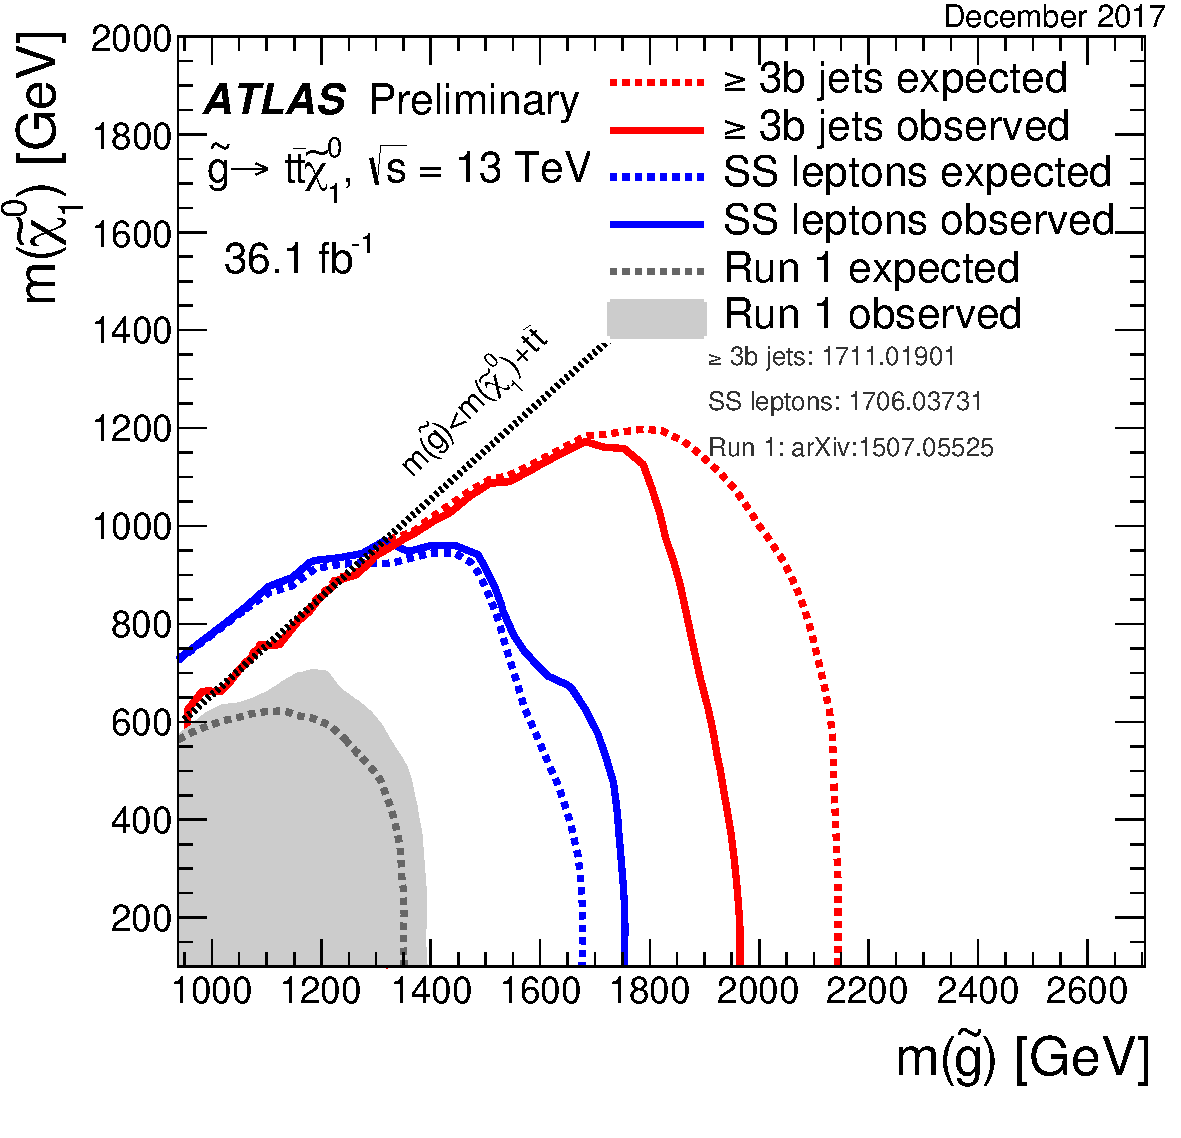
\includegraphics[width=0.65\textwidth]{./fig/limits/ATLAS_SUSY_Gtt.pdf}
\end{center}
\caption[ATLAS Gluino-mediated stop production limits]{ATLAS Gluino-mediated stop production limits in the $(m_{\tilde{g}}, m_{\tilde{chi}_1^0})$ plane.}
\label{fig:ATLASgluinolimits}
\end{figure}

\subsubsection{Direct stop pair production}

Figure \ref{fig:ATLASstoplimits} shows a summary of the dedicated ATLAS searches for top squark (stop) pair production based on 20 \ifb of p-p collision data taken at \cmotto TeV, and 4.7 \ifb of p-p collision data taken at \cmotto TeV \cite{atlas:stop0lep} \cite{atlas:stop2lep}. Exclusion limits at 95\% CL are shown in the $\left( m_{\tilde{t}_1}, m_{\tilde{\chi}^+_1} \right)$ plane. The dashed and solid lines show the expected and observed limits, respectively, including all uncertainties except the theoretical signal cross-section uncertainty. Three decay modes are considered separately with 100\% BR: 

\begin{itemize}
\item $\tilde{t} \rightarrow t \tilde{\chi}^0_1$ (7 TeV: \cite{atlas:stoplim_1} \cite{atlas:stoplim_2} \cite{atlas:stoplim_3}, 8 TeV \cite{atlas:stoplim_4} \cite{atlas:stoplim_5} \cite{atlas:stoplim_6}, where the $\tilde{t}_1$ is mostly right-handed)


\item $\tilde{t} \rightarrow W b  \tilde{\chi}^0_1$ (3-body decay for $m_{\tilde{t}} < m_t + m_{\tilde{\chi}^0_1} $, 8 TeV \cite{atlas:stoplim_4}\cite{atlas:stoplim_6}) 

\item  $\tilde{t} \rightarrow f f' b  \tilde{\chi}^0_1$ (4-body decay, 8 TeV \cite{atlas:stoplim_4}\cite{atlas:stoplim_7}). The region stop1 mass below 100 GeV has not been considered in \cite{atlas:stoplim_4} for the 4-body decay. 

\end{itemize}

\begin{figure}[htbp]
\begin{center}
%\includegraphics[width=0.65\textwidth]{./fig/limits/ATLAS_SUSY_Stop_tLSP.pdf}
\end{center}
\caption[ATLAS limits on direct stop production]{ATLAS limits on direct stop production in the $\left( m_{\tilde{t}_1}, m_{\tilde{\chi}^+_1} \right)$ plane.}
\label{fig:ATLASstoplimits}
\end{figure}



\subsubsection{Electroweak chargino-neutralino production}

Figure \ref{fig:ATLASewlimits} shows the summary of ATLAS searches for electroweak production of charginos and neutralinos based on 20 \ifb of p-p collision data at \cmotto TeV. Exclusion limits at 95\% confidence level are shown in the $\left( m_{\tilde{\chi}^+_1}, m_{\tilde{\chi}^0_1}  \right)$ plane. The dashed and solid lines show the expected and observed limits, respectively, including all uncertainties except the theoretical signal cross-section uncertainties. Four decay modes of the charginos and neutralinos are considered separately with 100\% branching fraction: 

\begin{itemize}

\item $\tilde{\chi}^+_1 \rightarrow \tilde{l} \nu (\tilde{\nu} l ) \rightarrow l \nu \tilde{\chi}^0_1 $, $\tilde{\chi}^0_2  \rightarrow \tilde{l} l (\tilde{\nu} \nu ) \rightarrow l l \tilde{\chi}^0_1 ( \nu \nu \tilde{\chi}^0_1  )$, resulting in BR(3 leptons)=50\% and BR(2 leptons)=100\% for $\tilde{\chi}^+_1 + \tilde{\chi}^0_2$ and $\tilde{\chi}^+_1 + \tilde{\chi}^+_1$ productions, respectively. The decays via sleptons and sneutrinos occur with 50\% probability each. 

\item $\tilde{\chi}^+_1 \rightarrow \tilde{\tau} \nu_{\tau} \tilde{\nu} \rightarrow \tau \nu \tilde{\chi}^0_1$,  $\tilde{\chi}^0_2  \rightarrow \tilde{\tau} \tau ( \tilde{\nu} \nu ) \rightarrow \tau \tau \tilde{\chi}^0_1 ( \nu \nu \tilde{\chi}^0_1   ) $, resulting in BR(3 taus)=50\% and BR(2 taus)=100\% for $\tilde{\chi}^+_1 + \tilde{\chi}^0_2$ and $\tilde{\chi}^+_1 + \tilde{\chi}^+_1$ productions respectively. The decays via staus and tau sneutrinos occur with 50\% probability each. 

\item $\tilde{\chi}^+_1 \rightarrow W  \tilde{\chi}^0_1$, $\tilde{\chi}^0_2  \rightarrow Z \tilde{\chi}^0_1$.

\item $\tilde{\chi}^+_1 \rightarrow W  \tilde{\chi}^0_1$, $\tilde{\chi}^0_2  \rightarrow H \tilde{\chi}^0_1$, where H is the Higgs boson and decays with the SM branching ratios.

\end{itemize}

\begin{figure}[htbp]
\begin{center}
%\includegraphics[width=0.65\textwidth]{./fig/limits/ATLAS_SUSY_EWSummary.pdf}
\end{center}
\caption[ATLAS Electroweak chargino-neutralino production limits]{ATLAS limits for Electroweak chargino-neutralino production in the $\left( m_{\tilde{\chi}^+_1}, m_{\tilde{\chi}^0_1}  \right)$ plane.}
\label{fig:ATLASewlimits}
\end{figure}

\begin{figure}[p]
\begin{center}
%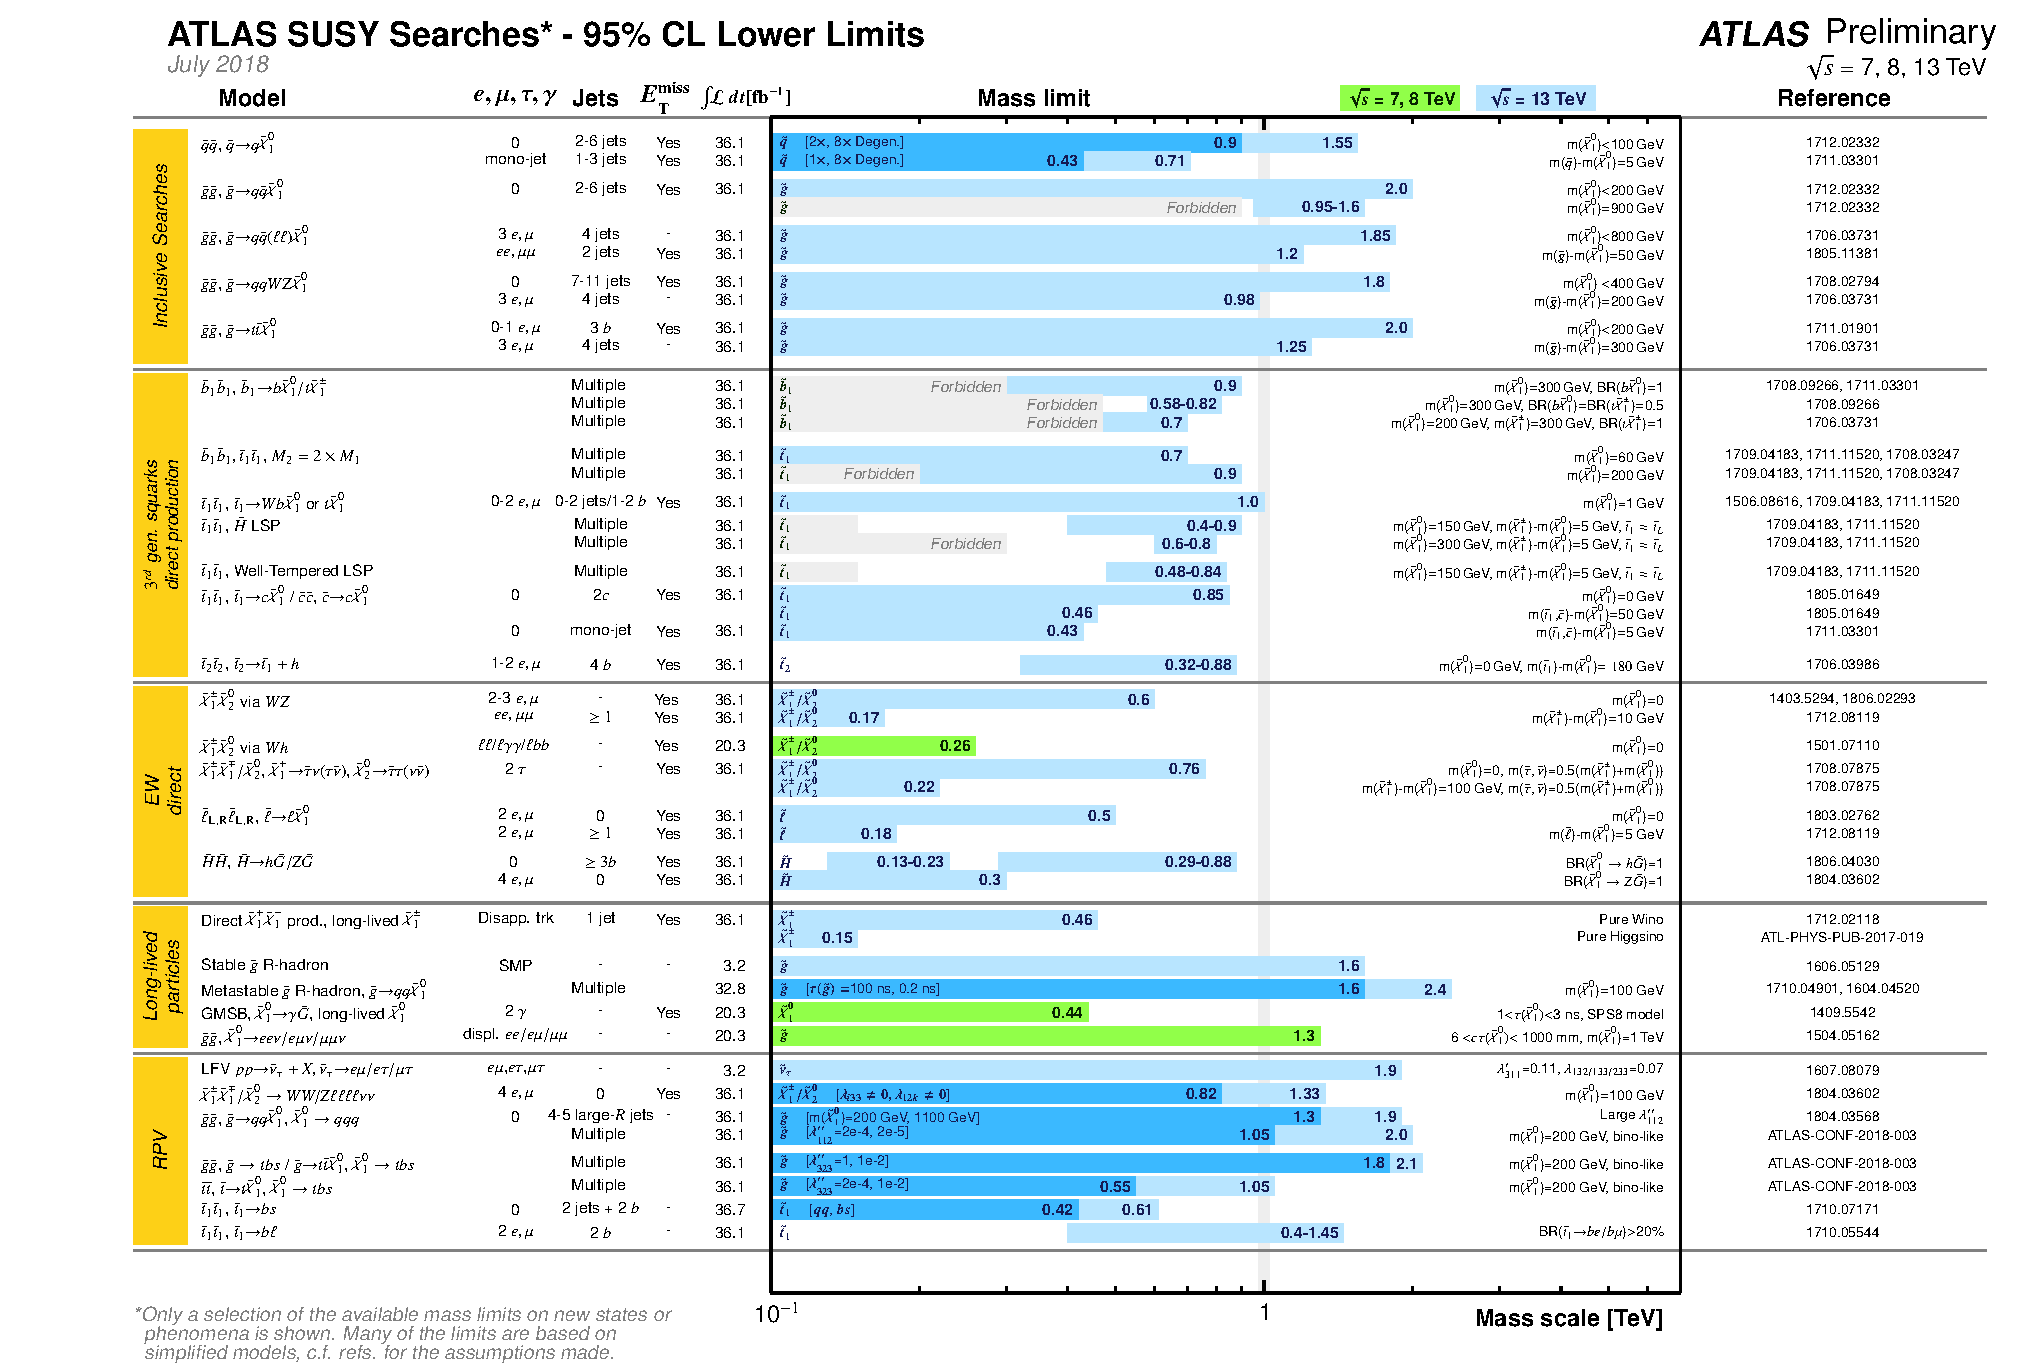
\includegraphics[width=\textwidth]{./fig/limits/ATLAS_SUSY_Summary.pdf}
\end{center}
\caption[Mass reach of ATLAS searches for Supersymmetry]{Mass reach of ATLAS searches for Supersymmetry.}
\label{fig:SUSYlimits}
\end{figure}


%%%%%%%%%%%%%%%%%%%%%%%%%%%%%%%%%%%%%%%%%%
%%%%%%%%%%%%%%%%%%%%%%%%%%%%%%%%%%%%%%%%%%







\chapter{Standard Model and Supersymmetry}
\label{chap:SMSUSY}

This chapter presents an introduction to the \gls{sm} of particle physics, the theory that nowadays best describes the subatomic world. In Section \ref{sec:smsusy:sm} a general overview of the \gls{sm} is given. Section \ref{sec:smsusy:bsm} discusses the limitations of the SM, and some of the theoretical extensions proposed to overcome them. Finally Section \ref{sec:smsusy:susy} focuses on Supersymmetry, arguably one of the most promising of these extensions. Throughout this chapter (as well as in the rest of this thesis) we will use natural units; we will thus use energy units to describe masses, as the speed of light ($c$) and the Planck constant ($\hslash$) are set to unity.


\section{The Standard Model of Particle Physics}
\label{sec:smsusy:sm}

The \gls{sm} is a renormalizable gauge quantum field theory based on the group $SU(3) \times SU(2) \times U(1)$. It was developed in the second half of the 20th century \cite{Glashow:1961tr, Weinberg:1967tq, Salam:1980jd}, and since then the description that it gives of the elementary particles and of their interactions has been accurately tested by several experiments. Many experimental discoveries have been guided by the \gls{sm} predictions, including the discovery of the top quark \cite{Abachi:1994td, PhysRevLett.74.2626} and up to the latest one, the observation of the Higgs boson at the \gls{lhc} in July 2012 \cite{Aad:2012tfa, Chatrchyan:2012xdj}. 

\subsection{Particle content of the Standard Model}

In the \gls{sm}, particles are described as excitations of quantum fields. In the following paragraphs, we introduce the quantum field theory description of fermions and bosons.

\subsubsection*{Fermions}

Matter constituents are half-integer spin fields (fermions). Fermions are further divided into two categories based on the type of interaction they experience:
\begin{description}
\item[Leptons] which experience only the electroweak interaction.
\item[Quarks] which experience both the electroweak and the strong interaction.
\end{description}

Both leptons and quarks come in three generations, and conventionally the numbering of these generations follows an order of increasing mass. A summary of the \gls{sm} fermions is presented in Table \ref{tab:sm_fermions}. While it is possible to observe free leptons, quarks exist only in bound states (hadrons); this is because of the confinement property of the strong interaction, discussed in Section \ref{sec:strong}. Hadrons built of three quarks have spin $\frac{1}{2}$ and are named barions, while mesons are formed by two quarks and have integer spin.


The free Lagrangian of a fermion is given by:

\begin{equation}
 \mathcal{L}_{free} = \bar{\psi} \left( i \gamma^{\mu} \partial_{\mu} - m \right) \psi \, , \
 \label{eq:sm:dirac}
\end{equation}

\noindent where $\psi$ is the fermion field, $m$ its mass, $\gamma$ are the Dirac matrices and $\partial_{\mu}$ is the four-momentum derivative. 

\begin{table}[h]
\centering
\begin{tabular}{c|ccc|ccc}
\hline
 & \multicolumn{3}{c|}{Leptons} & \multicolumn{3}{c}{Quarks} \\
\hline
\hline
Generation & Flavour & Charge & Mass [GeV] & Flavour & Charge & Mass [GeV]\\
\hline
\hline
\multirow{2}*{$1^{st}$} & $\nu_e$ & 0   & $< 2 \times 10^{-9}$  & $u$ & +2/3 & $2.2 \times 10^{-3}$ \\
                        & $e$     & -1  & $5.1 \times 10^{-4}$ & $d$ & -1/3 & $4.8 \times 10^{-3}$ \\
\hline  
\multirow{2}*{$2^{nd}$} & $\nu_\mu$ & 0   & $< 2 \times 10^{-9}$  & $c$ & +2/3 & $ 1.27 $ \\
                        & $\mu$     & -1  & $ 0.10566  $ & $s$ & -1/3 & $ 0.096 $ \\
\hline                 
\multirow{2}*{$3^{rd}$} & $\nu_\tau$ & 0   & $< 2 \times 10^{-9}$  & $t$ & +2/3 & $ 173.2 $ \\
                        & $\tau$     & -1  & $ 1.77 $ & $b$ & -1/3 & $ 4.66 $ \\
\hline  
                 
%\multirow{2}*{Weak} & $W^{+}$, $W^{-}$    &  +1, -1 &  	$80.385$ $\pm0.015$ \\%  & $10^{-6}$\\
 
\end{tabular}
\caption[Standard Model Ferimons]{Fermion content of the Standard Model. Each particle is listed with its electric charge and mass \cite{Patrignani:2016xqp}.} 
\label{tab:sm_fermions}
\end{table}


\subsubsection*{Bosons}

Particles with integer spin are referred to as bosons. In the \gls{sm}, force carriers are described through spin-1 fields. 
The \gls{sm} includes also a spin-0 particle, the Higgs boson. Is the interaction with the Higgs boson field that allows all the other elementary particles to acquire mass, as described in Section \ref{sec:smsusy:ew}.

The Klein-Gordon Lagrangian governs the kinematics of spin-0 neutral particles:

\begin{equation}
\mathcal{L}_{\rm{free}} = \frac{1}{2} \partial^\mu \phi \partial_\mu \phi - \frac{1}{2} m^2 \phi ^2 ,
\end{equation}

 
\noindent while in the case of charged particles (described through a complex field) the Lagrangian becomes:

\begin{equation}
\mathcal{L}_{\rm{free}} =  \partial^\mu \phi \partial_\mu \phi^* -  m^2 \phi \phi^* .
\end{equation}


\noindent The two equations above describe scalar particles. In the case of a vector field $A^\mu$, the expression of the Lagrangian is the following: 

\begin{equation}
\mathcal{L}_{\rm{free}} =  - \frac{1}{4} F^{\mu \nu}F_{\mu \nu} +  \frac{1}{2} m^2 A^\mu A_\mu \, .
\label{eq:lproca}
\end{equation}

\noindent This is the Proca Lagrangian. In the case of a particle with zero mass, this reduces to the Maxwell Lagrangian:

\begin{equation}
\mathcal{L}_{free} =  - \frac{1}{4} F^{\mu \nu}F_{\mu \nu} ,
\label{eq:lmax}
\end{equation}


\noindent where $F^{\mu \nu} = \partial^\mu A_\nu - \partial^\nu A_\mu$.

\subsection{Interactions and gauge invariance}

The \gls{sm} describes all the interactions among elementary particles, except for gravity, for which nowadays no renormalizable quantum field theory is formulated. Table \ref{tab:sm_interazioni} presents a summary of the \gls{sm} interactions and the properties of the corresponding force carriers. More details about the strong and electroweak interactions are given in the following sections.

\begin{table}[h]
\centering
\begin{tabular}{llcc}
\hline
Interaction & Carrier & Electric Charge & Mass [GeV] \\% & $\alpha$ \\
\hline
\hline
Strong & Gluons (g)  & 0 & 0 \\ % & 10 \\
\hline
Electromagnetic & Photon ($\gamma$) & $< 10^{-27}$ & 0 \\%& $10^{-2}$ \\
\hline
\multirow{2}*{Weak} & $W^{+}$, $W^{-}$    &  +1, -1 &  	$80.385$  \\% $\pm0.015$  & $10^{-6}$\\
 & $Z$  & 0 &  	$91.1876$  \\% & $\pm0.0021$ \\
\hline
\end{tabular}
\caption[Interaction in the Standard Model]{Interaction in the Standard Model. Here the different force carriers are listed, with their electric charges and masses \cite{Patrignani:2016xqp}.} %; $\alpha$ is the coupling constant of the different interactions.}
\label{tab:sm_interazioni}
\end{table}


The interaction terms in the \gls{sm} Lagrangian are introduced by promoting an already existing global symmetry of the Lagrangian ($\theta$) to a local one ($\theta(x)$) function of the space-time coordinates. 
In general, given a Lagrangian globally invariant under a symmetry group, the fields transform as:
\begin{equation}
\psi \rightarrow e^{ig\theta_k \tau_k} \psi  \; ,
\end{equation}

\noindent where $g$ is the coupling constant of the filed $\psi$ under the interaction and $\tau_k$ are the generators of the group and obey commutation relations: 
\begin{equation}
\left[ \tau_i, \tau_j \right] = i f_{ijk} \tau^k \; . 
\end{equation}

\noindent $f_{ijk}$ is the structure constant of the group and is always zero for Abelian groups. Promoting this gauge invariance to a global one ($\theta_k \rightarrow \theta_k(x)$) implies adding to the theory:
\begin{itemize}
\item A number of massless gauge fields $W^\mu_k$ equal to the number of generators of the symmetry group, that transform as 
\begin{equation}
W^\mu_k \rightarrow W^\mu_k - \partial^\mu \theta_k - g \epsilon_{klm} \theta^m W^\mu_m \; .
\end{equation}
\item A covariant derivative: 
\begin{equation}
D^\mu = \partial^\mu + ig\tau^kW^\mu_k \; ,
\end{equation}

\noindent that substitutes the standard derivative in the Lagrangian.
\item A free Lagrangian for the vector fields as in Equation \ref{eq:lproca}, with:
\begin{equation}
F^{\mu \nu}_k = \partial_\mu W_k^\nu - \partial_\nu W_k^\mu - g f_k^{lm} W^\mu_l W^\nu_m \; .
\end{equation}
\noindent Note that the last term, of second order in the field, is present only for non-Abelian symmetry groups, since it is proportional to the structure constant. This has non-trivial consequences as the second-order term leads to self-interaction among the gauge fields.
\end{itemize}


The \gls{sm} is a theory invariant under $SU(3)_{C} \times SU(2)_{L} \times U(1)_{Y}$. Imposing local invariance under $SU(3)_{C}$ leads to the theory of strong interactions, while $SU(2)_{L} \times U(1)_{Y}$ is the symmetry whose breaking gives origin to the electroweak interactions. 

\subsection{Strong interaction}
\label{sec:strong}

\gls{qcd} is the theory that describes strong interactions, based on the symmetry group $SU(3)_\mathrm{C}$, where the subscript C refers to the color, the quantum number associated with these interactions; this can assume three possible values denoted with red, blue and green. The observable states, hadrons, are color singlets, while quarks (anti-quarks) carry only one color (anti-color) charge. Since the symmetry group is non-Abelian, also the corresponding eight gauge bosons (gluons) carry a color charge (bi-color, with one color and one different anti-color) and therefore interact not only with quarks but also among themselves. Since $SU(3)_\mathrm{C}$ is believed to be an exact symmetry,  gluons are massless. 

The renormalization of a gauge theory leads to the definition of running coupling constants, whose value depend on the energy scale at which they are evaluated. In \gls{qcd}, at leading order the dependence of the coupling constant on the energy scale $Q$ is given by:

\begin{equation}
\alpha_\mathrm{s}(Q^2)=\frac{12\pi}{\left(11N_\mathrm{C}-2n_\mathrm{f}\right)\log{\frac{Q^2}{\Lambda_\mathrm{QCD}^2}}} \; , 
\label{eq:alfaQCD}
\end{equation}

\noindent where $N_\mathrm{C}$ is the number of colors, $n_\mathrm{f}$ is the number of quark flavors that are active (i.e. whose mass is lower than the energy scale) and $\Lambda_\mathrm{QCD}$ is the infrared cutoff scale that sets the limit of validity of the perturbative approximation. In \gls{qcd} $N_\mathrm{C} = 3$, so for $n_\mathrm{f}<16$ the coupling constant decreases with the increase of the energy scale of the process considered. This behavior has important consequences on the properties of the strong interaction:

\begin{itemize}
\item At high $Q^2$ (i.e. at small distances), $\alpha_\mathrm{s}$ becomes small enough for the perturbative approximation to be correct. In this case quarks and gluons behave as free particles (asymptotic freedom) \cite{PhysRevLett.30.1343, PhysRevLett.30.1346}.
\item When the momentum transfer is small (i.e. at large distances) $\alpha_\mathrm{s}$ is large; this gives rise to confinement: quarks can not be observed as isolated particles, as it is not possible to extract individual quarks from hadrons. When the distance between two quarks is increased, the potential energy increases as well, up to the point when it is energetically more favorable to create from the vacuum a quark-antiquark pair and thus a new hadron is formed.
\item In a collider experiment, quarks and gluons will create a collimated spray of hadrons (jets).
\end{itemize}

The evolution of the \gls{qcd} coupling constant with the energy scale has been verified experimentally, as shown in Figure \ref{fig:sm:alphas} \cite{Bethke:2012jm}.

\begin{figure}[ht]
\centering
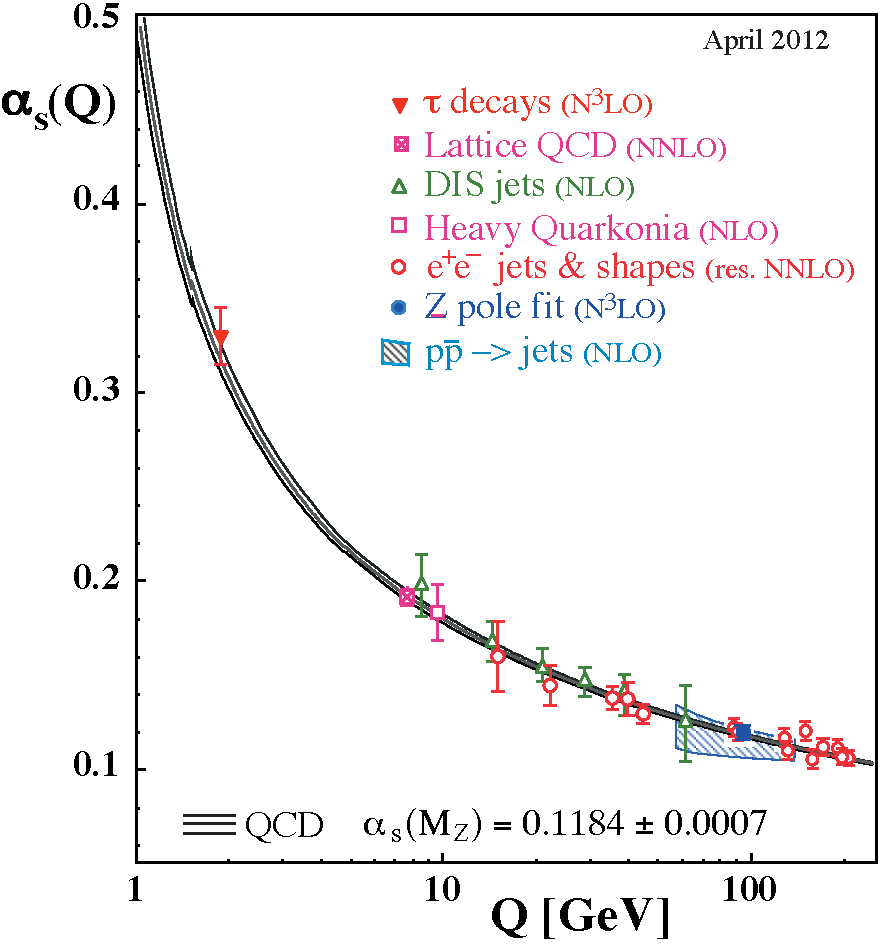
\includegraphics[width=0.5\textwidth]{figures/theory/asq-2011}
\caption{Evolution of the \gls{qcd} coupling constant $\alpha_\mathrm{s}$ with the energy scale. Figure from Ref \cite{Bethke:2012jm}.}
\label{fig:sm:alphas}
\end{figure}

\subsection{Electroweak interaction and Higgs-Englert-Brout mechanism}
\label{sec:smsusy:ew}

The theory of electroweak interactions is based on the symmetry group $SU(2)_\mathrm{L} \times U(1)_\mathrm{Y}$. This symmetry breaks at a scale around 100 GeV giving rise to the electromagnetic interaction, mediated by the photon, and to the weak interaction, mediated by the $Z$ and $W^{\pm}$ bosons  for neutral currents and charged currents respectively. The number of mediators, four, is the same as the number of generators of the symmetry group. 

The $SU(2)_\mathrm{L}$ part of the symmetry group governs the weak interactions, and the subscript L indicates that only left-handed particles participate to them. Left-handed and right-handed fields ($\psi_L$ and $\psi_R$ respectively) are defined through the chirality projectors $P_L$ and $P_R$:

\begin{equation}
\begin{aligned}
\psi_L = P_L \psi = \frac{(1 - \gamma_5)}{2} \psi, \\
\psi_R = P_R \psi = \frac{(1 + \gamma_5)}{2} \psi,
\end{aligned}
\label{eq:sm:LR}
\end{equation}

\noindent where $\gamma_5$ is defined as $\gamma_5 = i \gamma^0 \gamma^1 \gamma^2 \gamma^3 $. Looking back at Equation \ref{eq:sm:dirac}, it can be noted that, if we decompose the fermion field into its left-handed and right-handed components, the derivative term keeps $\psi_L$ and $\psi_R$ separated, while the mass term mixes them:
\begin{equation}
-m \bar \psi \psi = -m \bar \psi P_L^2 \psi - m \bar \psi P_R^2 \psi
	= -m \bar \psi_R \psi_L - m \bar \psi_L \psi_R \; .
\end{equation}


\noindent The covariant derivative for the  $SU(2)_\mathrm{L} \times U(1)_\mathrm{Y}$ group is:
\begin{equation}
\mathcal{D}^{\mu} = \partial^{\mu} + i \frac{g'}{2} B^\mu Y + ig W^\mu_k T^k \; ,
\label{eq:sm:covD}
\end{equation}

\noindent and substituting with this the regular derivative results in the interaction Lagrangian:
\begin{equation}
\mathcal{L}_{int}^{EW} = -\frac{g'}{2} \left( \bar{\psi} \gamma_\mu Y \psi \right) B^\mu - g \sum_k \left( \bar{\psi} \gamma_\mu T^k \psi  \right) W_k^\mu \; ,
\end{equation}

\noindent where we have introduced $T^k$, the weak isospin operator, and $Y$, the hypercharge operator (associated to the $U(1)_\mathrm{Y}$ group), and the respective coupling constants $g$ and $g'$. The quantum numbers of the $T^k$ and $Y$ operators relate to the electric charge $Q$ through the  Gell-Mann Nishijima relation:

\begin{equation}
Q = \frac{Y}{2} + T_3
\label{eq:sm:Q}
\end{equation}

\noindent where $Y$ is the hypercharge quantum number and $T_3$ is the quantum number of the third component of the isospin. 

In the case of an $SU(2)$ symmetry, it is not possible to add directly to the Lagrangian a mass term for the vector bosons of the form in Equation \ref{eq:lproca}, as it would spoil the $SU(2)$ local invariance. The Higgs-Englert-Brout mechanism \cite{Englert:1964et, Higgs:1964pj, Higgs:1964ia} solves this problem through \gls{ssb} of the $SU(2)_\mathrm{L} \times U(1)_\mathrm{Y}$ invariance. The \gls{ssb} is obtained by adding to the theory one extra isospin doublet of complex scalar components, the Higgs field:

\begin{equation}
	\Phi = \left( \begin{array}{c} \phi^+  \\ \phi^0 \end{array} \right) \; .
\end{equation}
%	= \frac{1}{\sqrt{2}} \left( \begin{array}{c} \phi_1 + i \phi_2 \\ \phi_3 + i \phi_4 \end{array} \right)

\noindent This doublet has hypercharge $Y=1$ and isospin $T=\frac{1}{2}$; the first component has positive electric charge, while the second one is electrically neutral. The Lagrangian for this new field includes a kinetic and a potential term:

\begin{equation}
	\mathcal{L}_{\Phi} = ( \mathcal{D}_{\mu} \Phi)^{\dagger} (\mathcal{D}^{\mu} \Phi) - V(\Phi) \; ,
	\label{eq:LHiggs}
\end{equation}

\noindent where $\mathcal{D}_{\mu}$ is the covariant derivative defined in Equation \ref{eq:sm:covD} and the potential $V(\Phi)$ is given by:

\begin{equation}
 V(\Phi) =  \mu^2 \Phi^{\dagger} \Phi + \lambda (\Phi^{\dagger} \Phi)^2 \, . 
	\label{eq:hpot}
\end{equation}

\noindent The two real parameters $\mu^2$ and $\lambda$ relate respectively to the mass term and the strength of the self-interaction term. The shape of the potential depends on the value of these parameters:
\begin{itemize}
\item If $\lambda < 0$, the potential does not present any stable minima, and this case is therefore unphysical.
\item If $\lambda > 0$ and $\mu^2 > 0$ there is only one solution to the minimization of the potential, $\Phi=0$. This case is shown in Figure  \ref{fig:sm:HiggsV_1}.
\item If $\lambda > 0$ and $\mu^2 < 0$, the field acquires a \gls{vev} as the minima is not at zero; it lies instead on the points of the circumference such that:
\begin{equation}
\Phi^{\dagger} \Phi = \frac{\mu^2}{2 \lambda}  \equiv \frac{v^2}{2} \; .
\end{equation}
\noindent Figure \ref{fig:sm:HiggsV_2} illustrates this case.
\end{itemize}


\begin{figure}[ht]
\centering
\subfigure[]{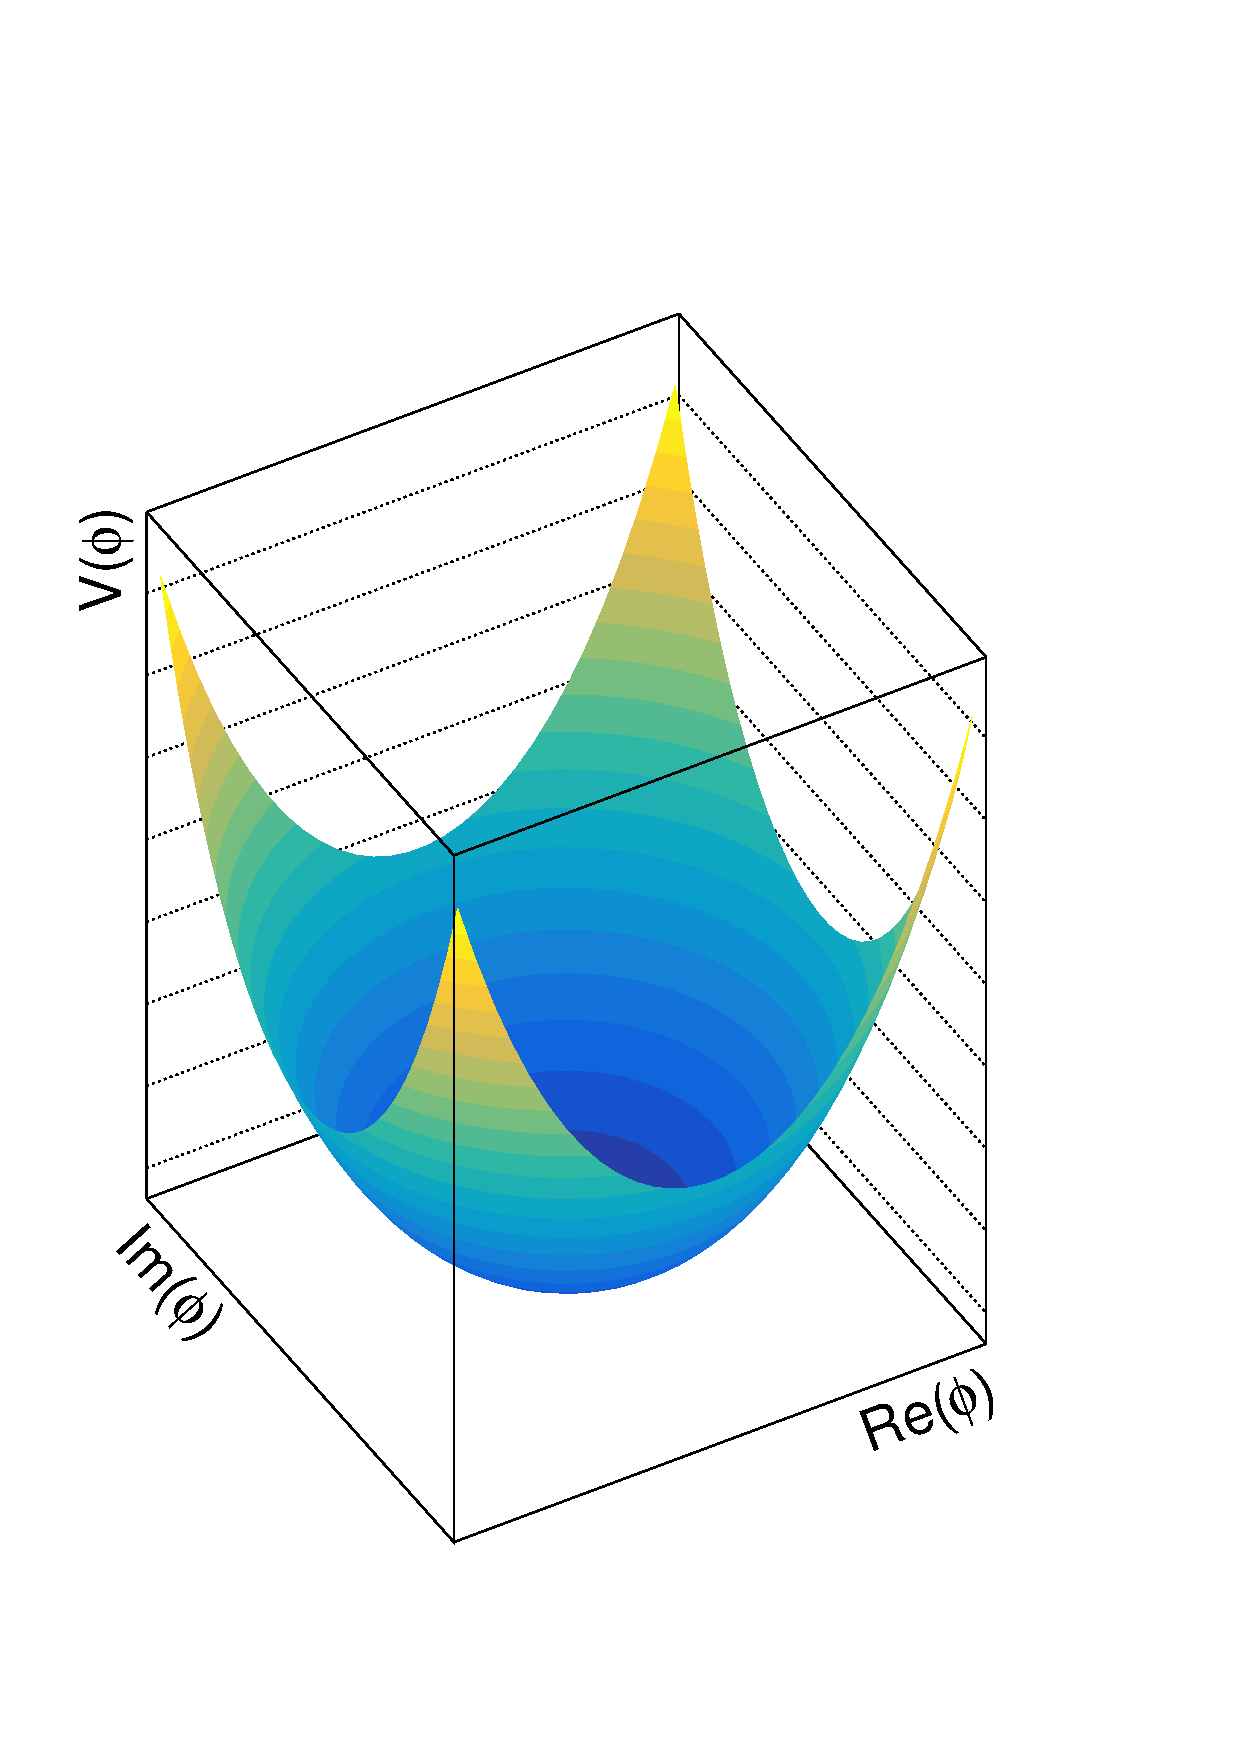
\includegraphics[width=0.49\textwidth]{produce_plots/sm/higgs_posmu2.pdf}\label{fig:sm:HiggsV_1}}
\subfigure[]{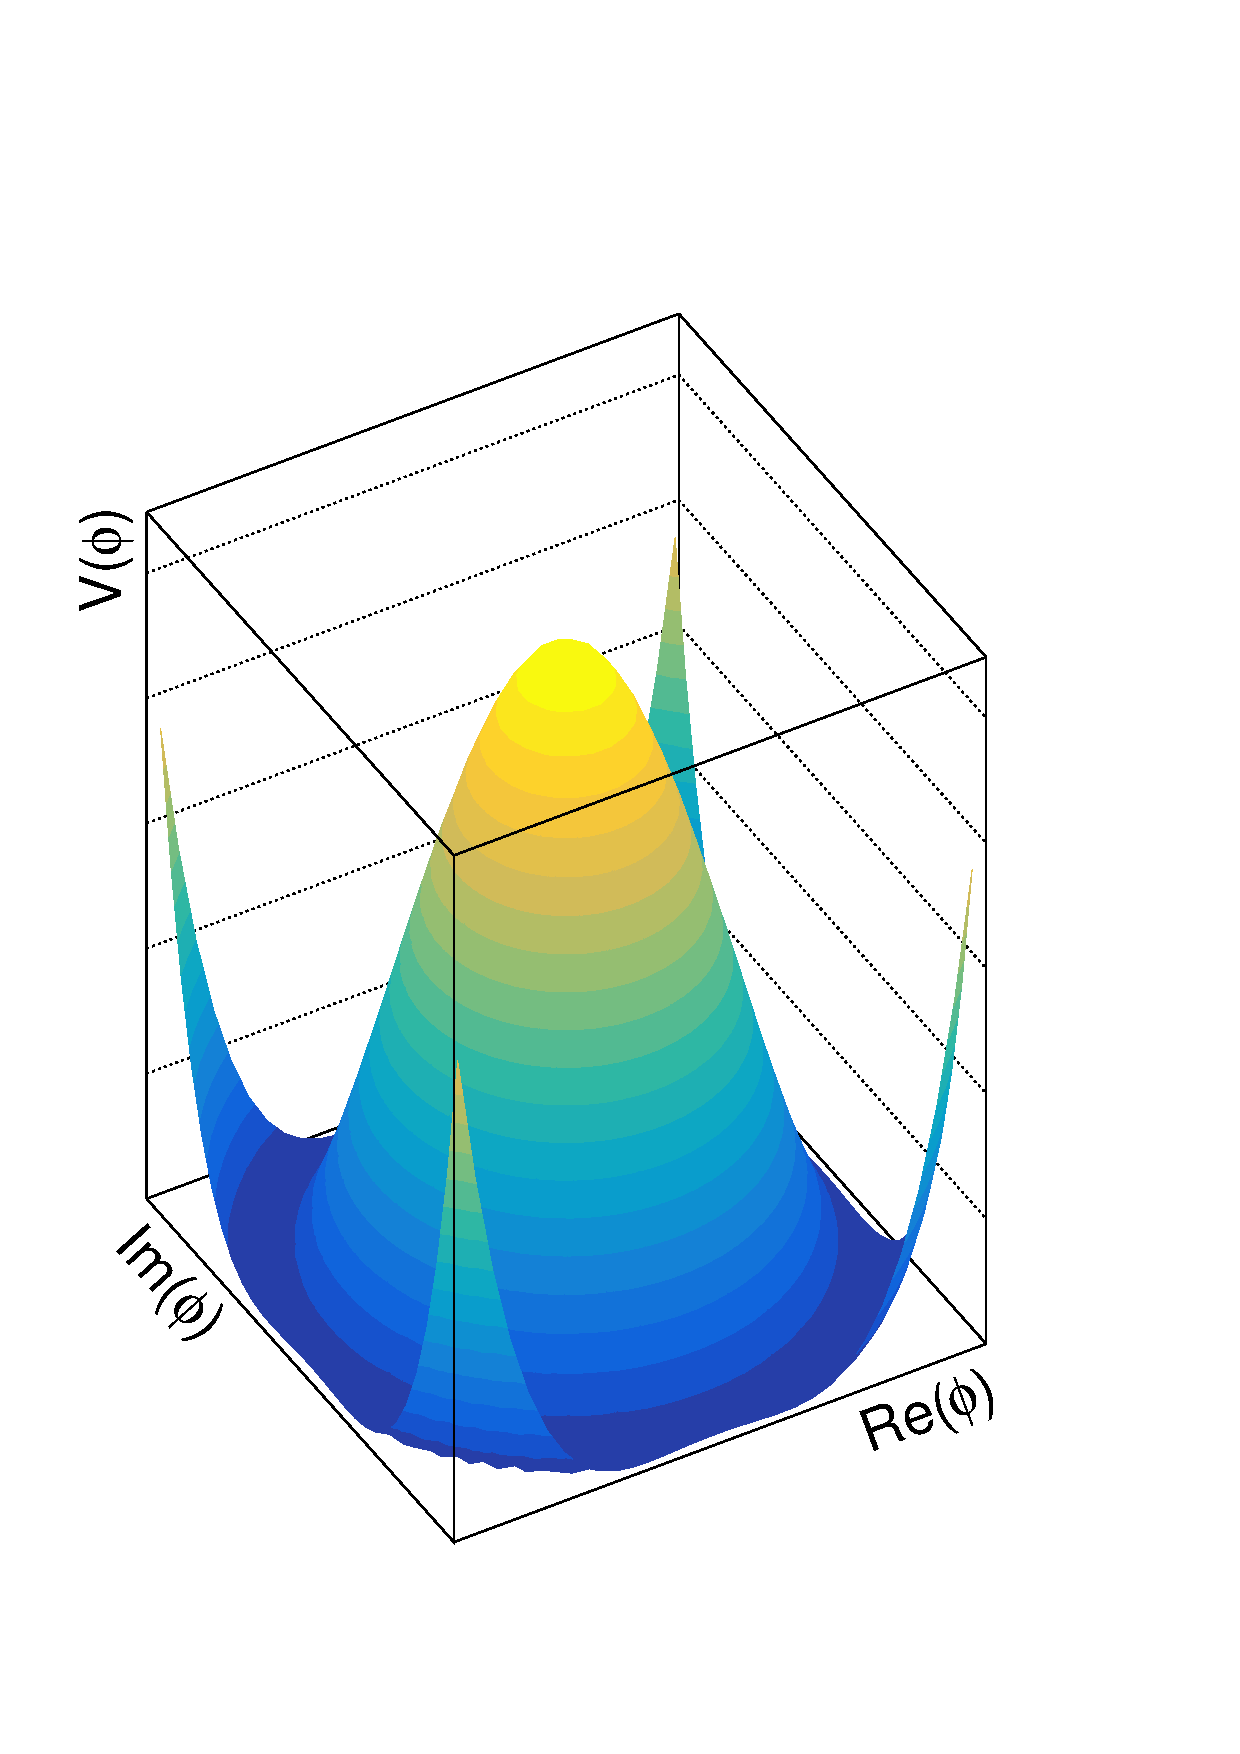
\includegraphics[width=0.49\textwidth]{produce_plots/sm/higgs_negmu2.pdf}\label{fig:sm:HiggsV_2}}
\caption{Higgs potential in the case \subref{fig:sm:HiggsV_1} $\lambda > 0$ and  $\mu^2 > 0$ and \subref{fig:sm:HiggsV_2} $\lambda > 0$ and $\mu^2 < 0$.}
\label{fig:sm:HiggsV}
\end{figure}

Up to this point the $SU(2)_\mathrm{L} \times U(1)_\mathrm{Y}$ symmetry is still intact, but the explicit choice of one of the infinite possible vacuum states for the Higgs field breaks the symmetry. According to the Goldstone theorem \cite{Goldstone:1962es}, the breaking of a continuous symmetry leads to the appearance of new massless scalar particles as field excitations. These new degrees of freedom are absorbed by the existing gauge bosons, thus giving them mass. To meet the experimental requirement of a massless photon, the choice of the Higgs vacuum has not to break the electromagnetic symmetry, $U(1)_{EM}$, so the component of the Higgs doublet that acquires a \gls{vev} is the neutral one:

\begin{equation}
	\Phi_0 = \frac{1}{\sqrt{2}} \left( \begin{array}{c} 0 \\ v  \end{array} \right) \, . \
\label{eq:hvphi}
\end{equation}

We can then expand the field $\Phi$ considering small excitations around the minimum:

\begin{equation}
	\Phi = \frac{e^{i \vec{\sigma} \cdot \vec{\theta}(x)/v }}{\sqrt{2}} \left( \begin{array}{c} 0 \\ v + \phi(x) \end{array} \right) \, ,
\label{eq:hvphi}
\end{equation}

\noindent where $\phi(x)$ is the physical field associated with the Higgs boson, $\vec{\sigma}$ the Pauli matrices and $\vec{\theta}(x)$ the three degrees of freedom absorbed to give masses to the $Z$ and $W^\pm$ bosons. Inserting Equation \ref{eq:hvphi} into Equation \ref{eq:LHiggs} relates the mass of the Higgs boson to the parameters in the potential:
\begin{equation}
m_H = \sqrt{- 2 \mu^2} = \sqrt{2 \lambda} v \; .
\label{eq:sm:Higgsmass}
\end{equation}

Since the numeric value of the $\mu^2$ and $\lambda$ parameters is not set, the theory does not predict a specific value for $m_H$. 
The physical mass eigenstates of the gauge bosons are a rotation of the interaction eigenstates, given by:

\begin{equation}
\begin{aligned}
W_\mu^\pm &= \frac{W_\mu^1 \mp W_\mu^2}{\sqrt{2}} \; , \\
A_\mu &= B_\mu \cos\theta_W + W^3_\mu \sin\theta_W \; ,  \\
Z_\mu &= W^3_\mu \cos\theta_W - B_\mu \sin\theta_W \; ,
\end{aligned}
\label{eq:wein}
\end{equation}

\noindent where we have introduced the Weinberg angle $\theta_W$ such that:
\begin{equation}
\tan\theta_W \equiv \frac{g'}{g} \; .
\end{equation}


The $(\mathcal{D}_{\mu} \Phi)^{\dagger} (\mathcal{D}^{\mu} \Phi)$ term in Equation \ref{eq:LHiggs} gives rise to the physical mass of the gauge bosons: once applied to the Higgs field, the covariant derivative in Equation \ref{eq:sm:covD} produces terms quadratic in the gauge fields, that we interpret as mass terms:

\begin{equation}
\mathcal{L}_{\Phi} = \left(1+\frac{\phi}{v}\right)^2 \,
\left\{ m_W^2\, W_\mu^\dagger W^\mu
+ \frac{1}{2}\, m_Z^2\, Z_\mu Z^\mu \right\}\, +\, \mathcal{L}_H \; , 
\end{equation}

\noindent where $\mathcal{L}_H$ denotes all the terms in $\mathcal{L}_{\Phi}$ that involve only the Higgs field: Higgs boson mass, cubic and quadratic self-interaction. Note that the coupling of the gauge bosons with the Higgs field is proportional to the square of the boson mass.
At tree level the resulting masses of the gauge bosons are:

\begin{equation}
\begin{aligned}
m_\gamma &= 0 \; ,\\
m_Z &= \frac{v \sqrt{g^2 + g'^2}}{2} \; , \\
m_W &= \frac{vg}{2} =  \cos\theta_W m_Z \; .
\end{aligned}
\end{equation}


Therefore, the Higgs-Englert-Brout mechanism generates automatically a mass term for the gauge bosons, that does not break the global underlying $SU(2)_\mathrm{L} \times U(1)_\mathrm{Y}$ symmetry. The Higgs field is used also to make fermion mass terms arise, but in this case it is necessary to postulate a Yukawa interaction between the Higgs and fermion fields. The fermion masses are assumed to be proportional to the strength of the coupling and, unlike the masses of the gauge bosons, they are not related to other parameters of the theory. While the Higgs field itself is enough to give mass to down-type fermions, the mass term for the up-type fermions  requires the introduction of the complex conjugate of the Higgs field ($\Phi_C$):

\begin{equation}
 \Phi_C = i \sigma^2 \Phi^* 
	= i \left( \begin{array}{cc} 0 & -i \\ i & 0 \end{array} \right) 
	\left( \begin{array}{c} \phi^- \\ \phi^{0*} \end{array} \right)
	= \left( \begin{array}{c} \phi^{0*} \\ - \phi^- \end{array} \right) \; ,
\end{equation}

\noindent If we identify as $g_f$ the coupling of the fermion $f$ to the Higgs field (Yukawa coupling), the additional part of the Lagrangian that generates the fermion masses is:

\begin{equation}
\begin{aligned}
\mathcal{L}_{Yukawa} &= - \left[  y_d \left( \bar{u}_L \,\, \bar{d}_L  \right) \Phi d_R +  y_u \left( \bar{u}_L \,\, \bar{d}_L  \right) \Phi_C u_R \right] + h.c. \\
&= - \frac{1}{\sqrt{2}} \left[  y_d \left( v + \phi \right) \bar{d}_L d_R + h.c. + y_u \left( v + \phi \right) \bar{u}_L d_u + h.c. \right]  \; .
\end{aligned}
\end{equation}

\noindent In this equation we can now easily identify the fermion mass terms, of the form:

\begin{equation}
m_f =  \frac{v}{\sqrt{2}} y_f \; .
\end{equation}

\noindent Note that, in the case of fermions, the coupling to the Higgs boson is directly proportional to the fermion mass.The matrices $y_f$ are not necessarily diagonal, but they can be diagonalized through a unitary transformation, which we can interpret as the transformation that relates the mass eigenstates to the weak interaction eigenstates. In the quark sector, this transformation is encoded in the \gls{ckm} matrix \cite{Cabibbo:1963yz, Kobayashi:1973fv}, that describes the mixing of the down-type quarks. In the \gls{sm} with three generations of fermions, the \gls{ckm} matrix is specified by three angles and one complex phase that provides the only source of CP violation.

\subsection{Measured properties of the Higgs boson}

The value of the Higgs boson mass is not predicted by the \gls{sm}, but it can be measured and, once it is know, the Higgs boson production cross-section and decay fractions can be predicted accurately. These predictions can be verified experimentally, providing hints toward believing that the discovered boson is indeed the \gls{sm} Higgs boson. In 2015 the ATLAS and CMS collaborations published a combined measurement of the Higgs boson mass \cite{Aad:2015zhl}:
\begin{equation}
m_H = 125.09 \pm 0.21 (\mathrm{stat.}) \pm 0.11 (\mathrm{syst.}) \;\; \mathrm{GeV}.
\end{equation}

\noindent This result uses the full Run 1 ATLAS and CMS data, analyzed in the $h \rightarrow \gamma \gamma$ and $h \rightarrow ZZ \rightarrow 4 \; \mathrm{leptons}$ channels.


The discussion of the Higgs mechanism in Section \ref{sec:smsusy:ew} highlights interesting properties of the interactions involving the Higgs boson. In particular, the strength of its coupling with fermions and bosons is proportional respectively to the mass and the square of the mass of the particle involved. 
This is reflected on the \glspl{br}: they are high for the decay to particles with the highest mass that are kinematically allowed.
While the top quark mass is too large to have the decay $h \to t\bar{t}$, the large top Yukawa coupling leads to loop-induced couplings of the Higgs boson to massless particles (gluons and photons); these are of phenomenological interest as they lead to the main production mode (gluon-gluon fusion) and to the $h \to \gamma \gamma$ decay mode, which has a low \gls{br} but leads to a very clean signature and was one of the key channels for the Higgs boson discovery. 
%The theoretical \glspl{br} for a Higgs boson mass of 125.09 GeV are reported in Table \ref{tab:SMBranchingFractions}. 

%\begin{table}[htbp]
%\begin{center}
%\begin{tabular}{clcr@{\hskip 0.4ex}l} \\ 
%\hline
% &    Decay mode &\multicolumn{3}{c}{Branching fraction [\%]}  \\  \hline
% \hline
% &     $H \rightarrow b\bar{b}$       & &   $57.5$&${}\pm 1.9$    \\
% &     $H \rightarrow WW$       & &   $21.6$&${}\pm 0.9$   \\
% &     $H \rightarrow gg$       & &   $8.56$&${}\pm 0.86$  \\
% &     $H \rightarrow \tau \bar{\tau}$       & &   $6.30$&${}\pm 0.36$  \\
% &     $H \rightarrow c\bar{c}$       & &   $2.90$&${}\pm 0.35$  \\
% &     $H \rightarrow ZZ$       & &   $2.67$&${}\pm 0.11$  \\
% &     $H \rightarrow \gamma \gamma$       & &   $0.228$&${}\pm 0.011$  \\
% &     $H \rightarrow Zg$       & &   $0.155$&${}\pm 0.014$  \\
% &     $H \rightarrow \mu \bar{\mu}$       & &   ~~$0.022$&${}\pm 0.001$  \\ 
%\hline
%\end{tabular} 
%\end{center}
%\caption{Standard Model predictions for the decay \glspl{br} of a Higgs boson with a mass of 125.09~GeV, together with their uncertainties~\cite{Heinemeyer:2013tqa}. Table follows Ref. \cite{Khachatryan:2016vau}.}
%\label{tab:SMBranchingFractions}
%\end{table} 
The theoretical production cross-section and \glspl{br} for a Higgs boson with mass between 120 and 130 GeV are reported in Figure \ref{fig:sm:h_xsec_br}.

\begin{figure}[ht]
\centering
\subfigure[]{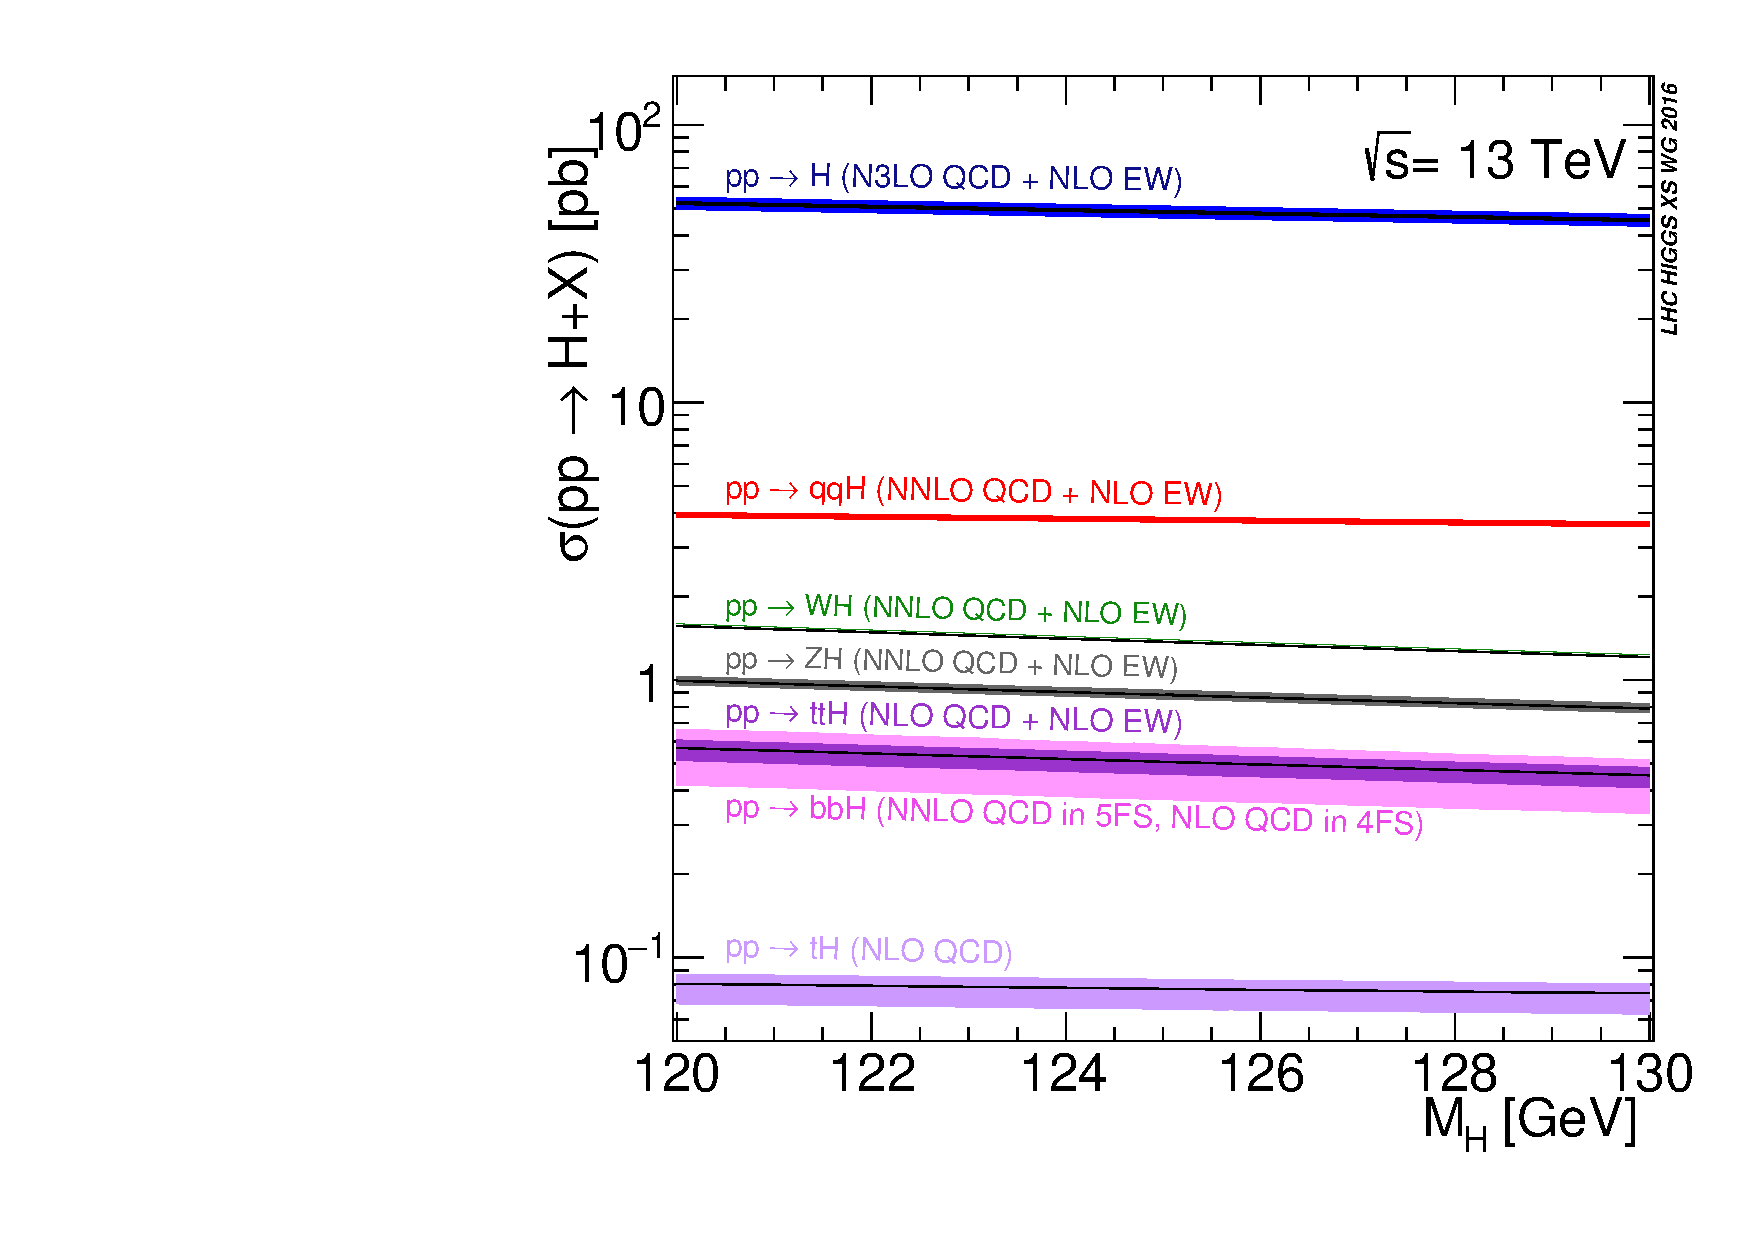
\includegraphics[width=0.49\textwidth]{figures/theory/plot_13tev_H_sqrt}\label{fig:sm:h_xsec_theo}}
\subfigure[]{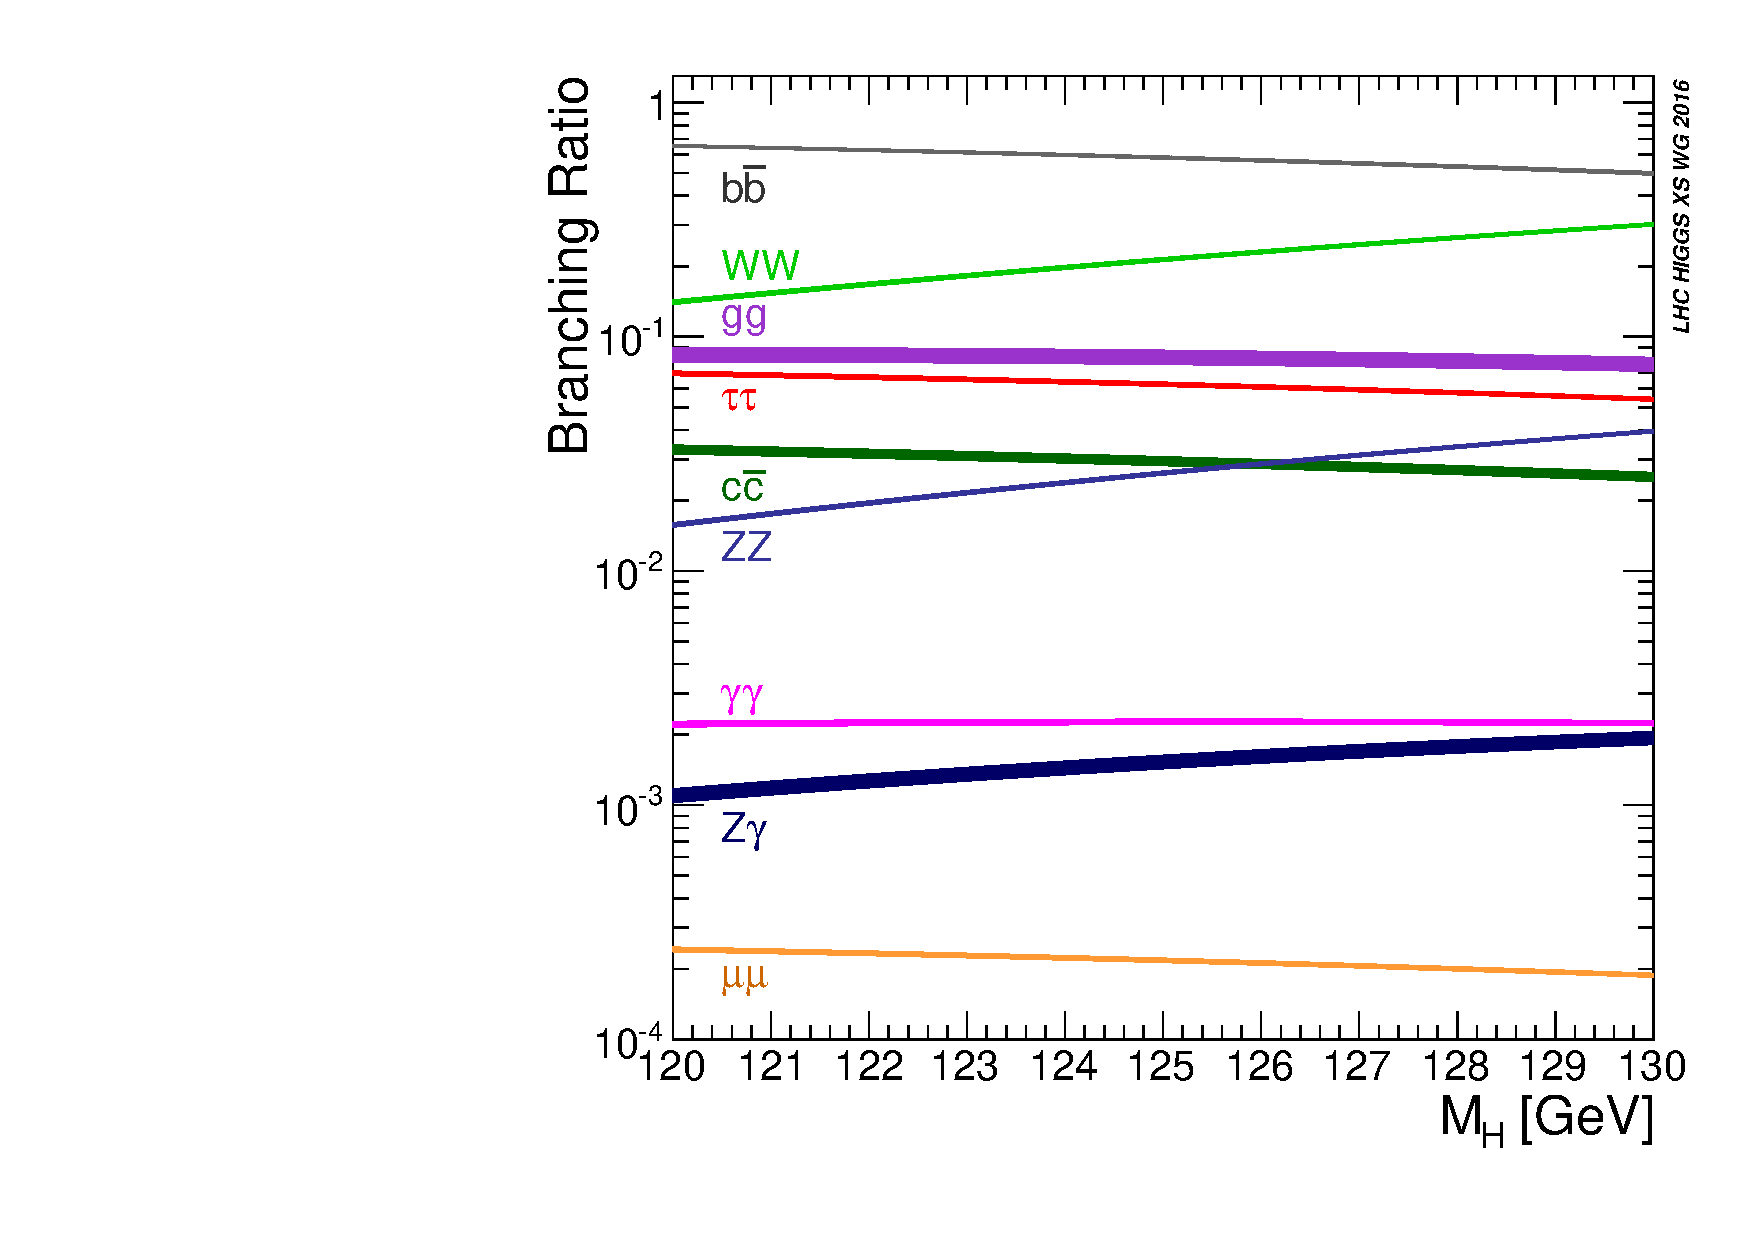
\includegraphics[width=0.49\textwidth]{figures/theory/SMHiggsBR_120-130.pdf}\label{fig:sm:h_br_theo}}
\caption{
\subref{fig:sm:h_xsec_theo} Higgs boson production cross-section at 13 TeV for a mass range between 120 and 130 GeV.
\subref{fig:sm:h_br_theo} Higgs boson \gls{br} for a mass range between 120 and 130 GeV.
Figures from Ref.  \cite{deFlorian:2016spz}.}
\label{fig:sm:h_xsec_br}
\end{figure}

The production cross-section is found to be in agreement with the \gls{sm} predictions within uncertainties. Figure \ref{fig:sm:h_xsec} shows the best fit value of Higgs production cross-section times \gls{br} in the different production and decay modes \cite{Khachatryan:2016vau}. Also the relation between the fermion or boson mass and the Higgs coupling has been verified experimentally, as show in Figure \ref{fig:sm:h_mass}. 

\begin{figure}[ht]
\centering
\subfigure[]{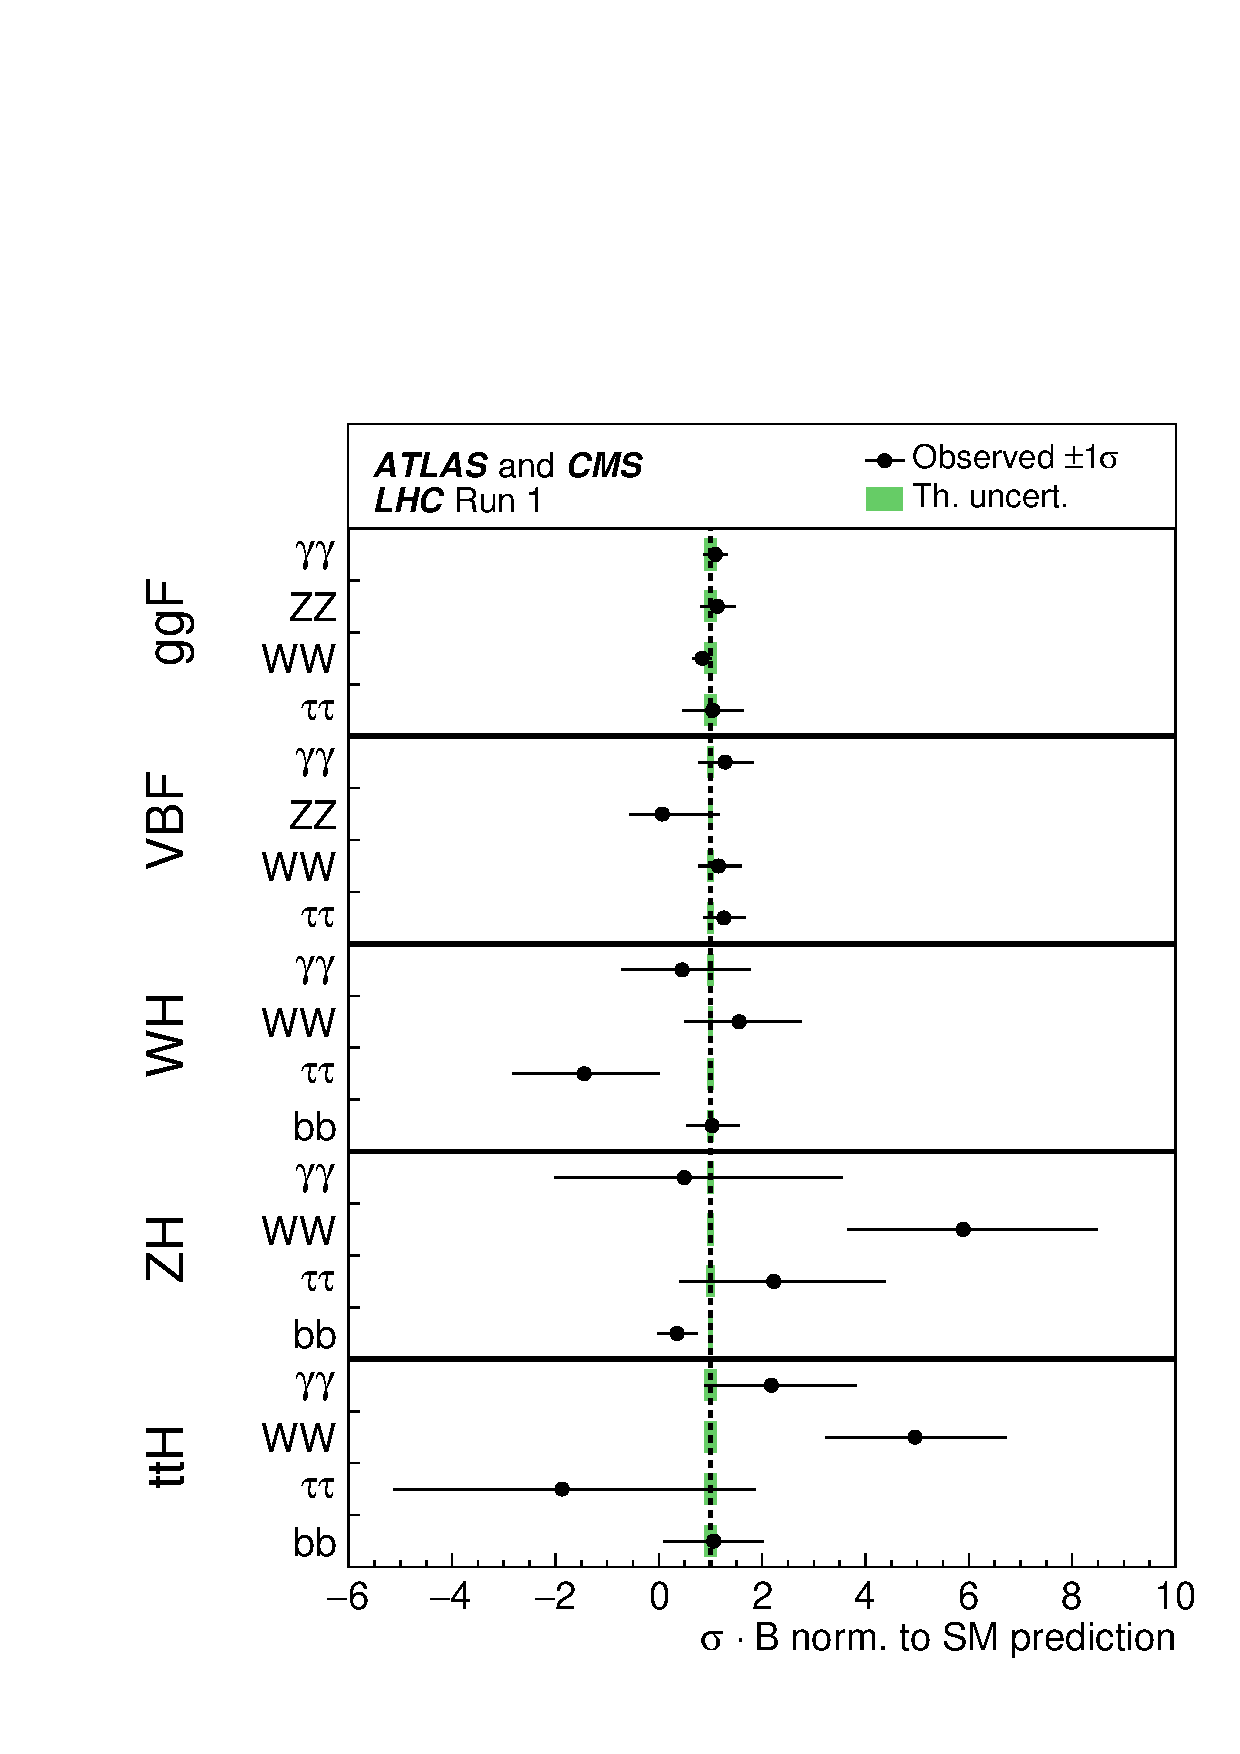
\includegraphics[width=0.49\textwidth]{figures/theory/CMS-HIG-15-002_Figure_007}\label{fig:sm:h_xsec}}
\subfigure[]{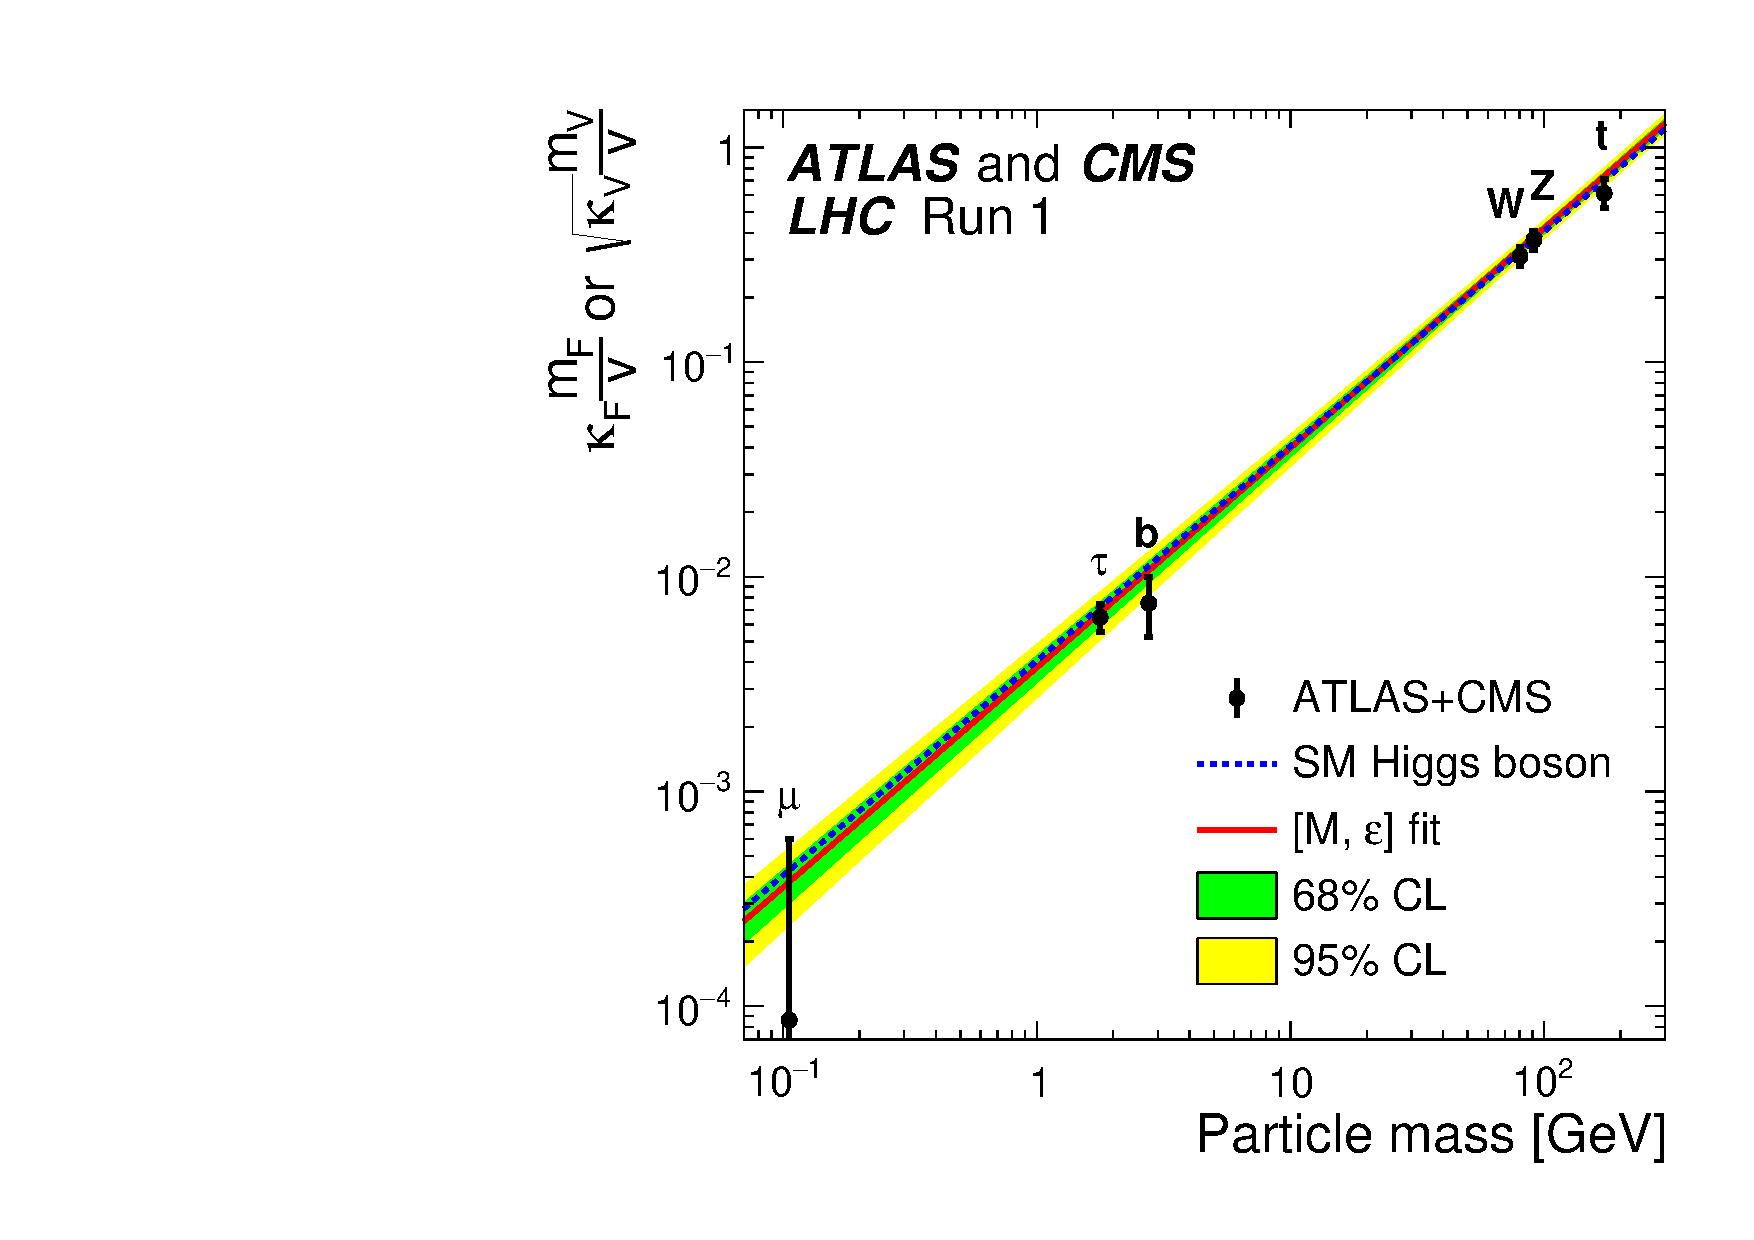
\includegraphics[width=0.49\textwidth]{figures/theory/CMS-HIG-15-002_Figure_019}\label{fig:sm:h_mass}}
\caption{\subref{fig:sm:h_mass} Best-fit values as a function of particle mass for the combination of Run 1 ATLAS and CMS data. \subref{fig:sm:h_xsec} Best-fit value of Higgs production cross-section times \gls{br} in different production and decay modes. Figure from Ref.  \cite{Khachatryan:2016vau}.}
\label{fig:sm:h_couplings_mass}
\end{figure}

 


\section{Limitations of the Standard Model and how to extend it}
\label{sec:smsusy:bsm}

Despite its undeniable success in describing the subatomic world, the \gls{sm} has some limitations that suggest it should be considered as the low-energy approximation of a more general theory. Nowadays there is no perfect candidate to fill the role of this general theory, but the shortcomings of the \gls{sm} highlight the characteristics this theory should have. Section \ref{sec:sm:missingpieces} discusses the experimental observations that are not accounted by the \gls{sm} framework, whose lacking is an objective limit of the \gls{sm}. In section \ref{sec:sm:aesthetics} we review some other features that the \gls{sm} is missing that, while not being strictly necessary, would be desirable in a general theory. Some theories and models candidate to extend the \gls{sm} are briefly presented in Section \ref{sec:sm:extensions}.

\subsection{Unexplained phenomena}
\label{sec:sm:missingpieces}

The \gls{sm} lacks an explanation for some well established experimental phenomena that are listed in the next paragraphs.

\subsubsection*{Neutrino Masses}

Neutrino oscillations \cite{PhysRevLett.81.1562} are possible only if there is a mass difference between the three neutrino generations, which automatically implies non-zero masses for at least some neutrinos. Although neutrino mass terms could be accommodated by the \gls{sm} through right-handed neutrinos or a description of neutrinos as Majorana particles, the basic formulation of the \gls{sm} describes neutrinos as massless particles.

\subsubsection*{Dark Matter and Dark Energy}

The \gls{sm} describes only baryonic matter; this accounts for about 5\% of the energy density in the universe. Even though no direct observation of it has been made so far, we know there is also another type of matter, that does not have electromagnetic interactions and  is about five times more abundant than ordinary matter.  Since this type of matter does not reflect light, it is referred to as dark matter. The presence of dark matter has been postulated for the first time from the rotational velocity of galaxies \cite{Zwicky:1937zza}, but this evidence has now been confirmed also by other observations, including the analysis of the cosmic microwave background from the WMAP and Planck collaborations \cite{Larson:2010gs,Ade:2013zuv}. The sum of baryonic and dark matter accounts for about 32\% of the of the energy density in the universe. 
The remaining 68\%, known as dark energy, is the energy responsible for the accelerated expansion of the universe. While some extensions of the \gls{sm} provide candidates for dark matter, at the moment no theory provides a compelling explanation for dark energy.


\subsubsection*{CP Violation}

CP-violating processes are needed in order to generate the observed asymmetry between the matter and the anti-matter content of our universe. While the \gls{sm} provides one source of CP violation with the complex phase in the \gls{ckm} matrix mentioned in Section \ref{sec:smsusy:ew}, this is not enough and additional sources are needed in order to explain the observed asymmetry.

\subsubsection*{Gravity}

Gravity is the only force acting on elementary particles that is not described by the \gls{sm}. In fact, not only is not described by the \gls{sm}, but the simple attempt to quantize gravity through a spin-2  mediator (graviton) leads to a non-renormalizable theory. The strength of gravity is expected to be comparable to that of the other forces at the Planck scale ($\Lambda_{Planck}$, $\approx 10^{19}$ GeV). 

\subsection{Aesthetic shortcomings}
\label{sec:sm:aesthetics}

While the previous section discusses objective shortcomings of the \gls{sm}, there are also some aesthetic criteria that the \gls{sm} does not seem to satisfy. These are mostly based on the concept of Naturalness: unless there is a good reason, the parameters of a "beautiful" theory should be all of the same order of magnitude, and a theory where instead the parameters are bound to assume very specific and different values (fine tuning) seems "unnatural". It is important to notice that this naturalness requirement is subjective, as well as the amount of fine tuning allowed for a theory to be considered natural.


\subsubsection*{Hierarchy Problem}

The expression for the mass of the Higgs boson in Equation \ref{eq:sm:Higgsmass} contains only the tree-level contribution. The proper computation should include the radiative contributions from all the particles that couple with the Higgs boson, directly or indirectly (see below). A fermion, whose Yukawa coupling leads to the interaction $-y_f \phi \bar{f} f$, will produce a correction to the Higgs boson mass with a divergent integral; this can be computed e.g. with a cut-off regularization, and in this case the resulting correction to the Higgs boson mass, shown in Figure  \ref{fig:sm:h_corr_fermion}, is:
\begin{equation}
\Delta m_H^2 \>=\>  
-{|y_f|^2\over 8 \pi^2} \Lambda_{UV}^2 + \mathcal{O}(\ln \Lambda_{UV} ) \; ,
\label{eq:divhf}
\end{equation}

\noindent where $\Lambda_{UV}^2$ is the cut-off scale, identified with the limit of validity of the theory. If we assume that no physics \gls{bsm} is present up to $\Lambda_{Planck}$, having corrections to the mass proportional to $\Lambda_{Planck}$ requires a fine tuning of the parameters of the order of $\frac{m_H}{\Lambda_{Planck}} \approx 10^{-17}$. This is due to the strong hierarchy of the scales involved (hierarchy problem) \cite{Weinberg:1975gm, PhysRevD.20.2619, PhysRevD.14.1667, tHooft:1979rat}. Since the correction to the mass is proportional to the Yukawa coupling of the fermion, it is clear that the most important correction is the one given by the top quark, whose Yukawa coupling is $y_t \approx 1$. % 0.996 

Despite this, it can still be argued that the appearance of the $\Lambda_{UV}$ divergence is connected more to the regularization scheme rather than to the theory itself. But even in this case, the value of 125 GeV for the Higgs boson mass remains difficult to justify. The \gls{sm} Lagrangian does not have any symmetry that prevents the Higgs boson to couple to new \gls{bsm} particles. If we assume the existence of a complex scalar that couples with the Higgs field through $ -y_S|\phi|^2 |S|^2$, the correction to the Higgs propagator, shown in Figure \ref{fig:sm:h_corr_scalar}, is given by:

\begin{equation}
\Delta m_H^2 \>=\> {y_S\over 16 \pi^2}
\left [\Lambda_{UV}^2 - 2 m_S^2
\> {\rm ln}(\Lambda_{UV}/m_S) + \ldots
\right ] \; .
\label{eq:divhs}
\end{equation}

\noindent Beside the first term, proportional to $\Lambda_{UV}^2$, that can be thought as a consequence of the cut-off regularization, we also have a second  term proportional to $m_S^2$. If we assume that \gls{bsm} physics exists and that, since it has not yet been observed, $m_S$ must be large, this contribution drives $m_H$ to high values. A similar argument applies even if the new \gls{bsm} sector and the Higgs field do not couple directly but, for example, share a gauge interaction.

\begin{figure}[ht]
\centering
\subfigure[]
{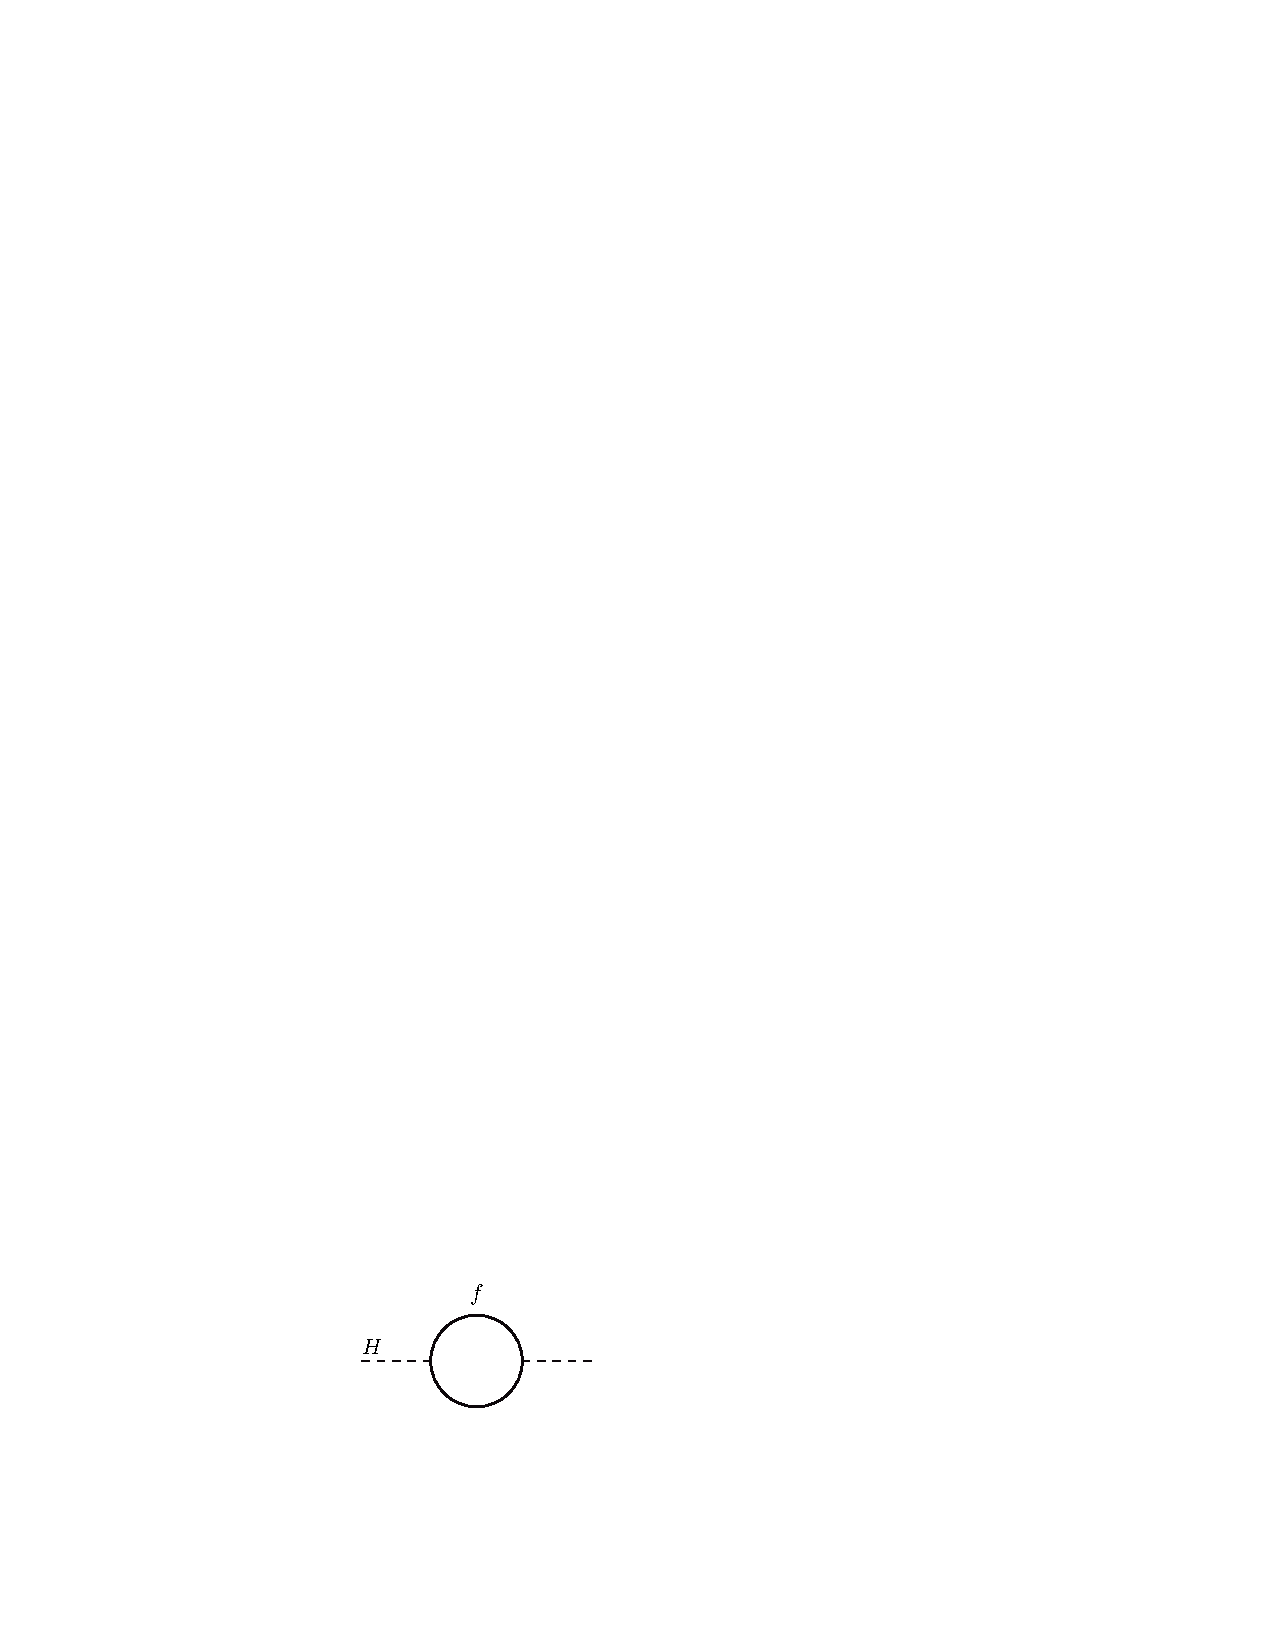
\includegraphics[width=0.36\textwidth]{figures/theory/h_corr_f.pdf}\label{fig:sm:h_corr_fermion}}
\subfigure[]{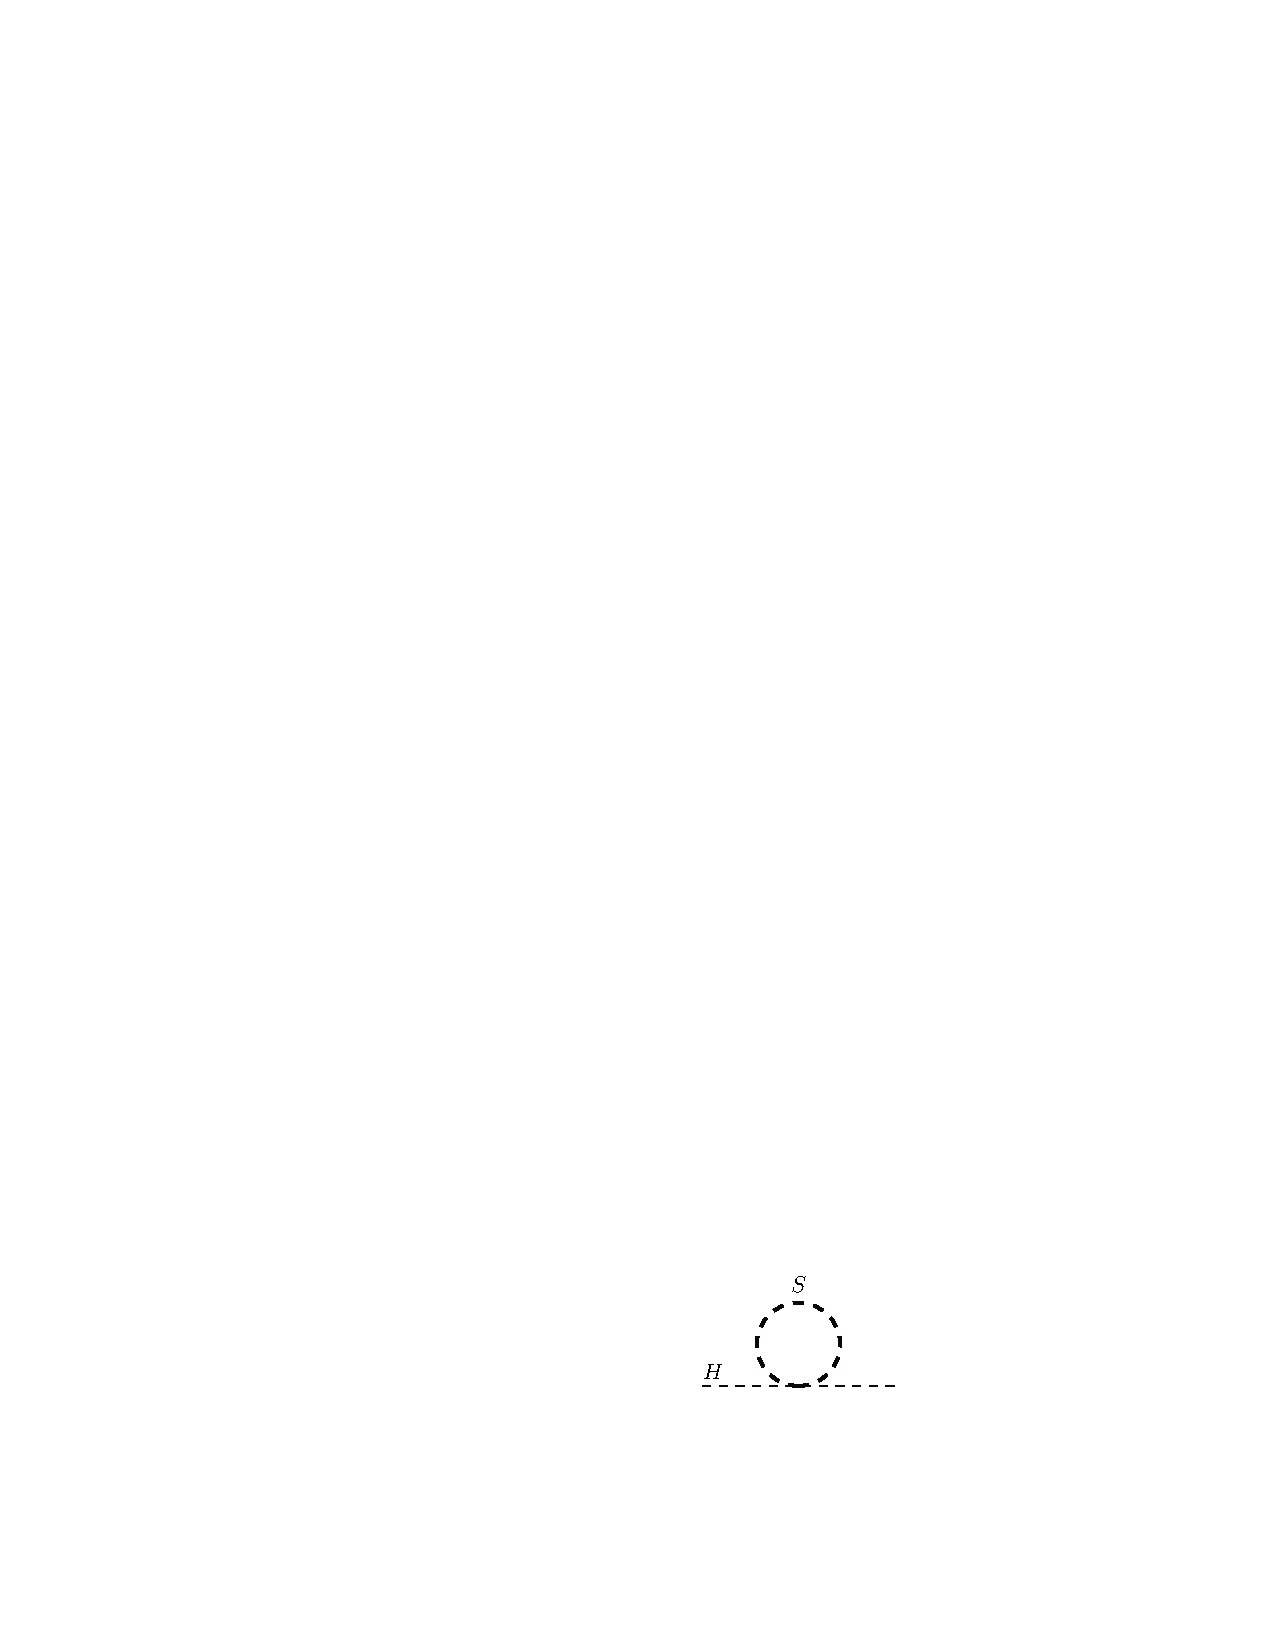
\includegraphics[width=0.36\textwidth]{figures/theory/h_corr_s.pdf}\label{fig:sm:h_corr_scalar}}
\caption{Correction to the Higgs boson propagator form the interaction with \subref{fig:sm:h_corr_fermion} a fermion and \subref{fig:sm:h_corr_scalar} a scalar. Figure from Ref. \cite{Martin:1997ns}.}
\label{fig:sm:h_corr}
\end{figure}

\subsubsection*{Fermion Mass Hierarchy} 

Fermion masses are less sensitive than the Higgs boson mass to the cut-off scale as the divergence is only logarithmic. Nevertheless, it is striking how strong the fermion Yukawa coupling hierarchy is: even if we don't consider neutrinos, fermion masses span about six orders of magnitude, without any apparent reason.

\subsubsection*{Unification of Coupling Constants}

The \gls{sm} coupling constants of the $SU(3)_\mathrm{C}$, $SU(2)_\mathrm{L}$ and $U(1)_\mathrm{Y}$ groups have a different evolution, and the extrapolation of their values at very high energies suggests a common value at a scale $M_{GUT} \approx 10^{15}-10^{16}$ GeV, after which the different couplings should unify. However, if the only particles involved in the computation of the evolution of the coupling constants are the \gls{sm} ones, there is no exact crossing point, as shown in Figure \ref{fig:susy:gut_0}.

\subsection*{Strong CP Problem}

The most general \gls{sm} \gls{qcd} Lagrangian should include also a CP-violating angle, and this would not spoil renormalizability. The presence of this term would have directly measurable physical consequences, for example a non-zero electric dipole moment for the neutron (nEDM). The tight  limits on the nEDM ( $< 3.6 \times 10^{-26}$ e cm at 95\% CL \cite{PhysRevD.92.092003}) translate into upper limits on the parameter regulating the CP-violating term of the \gls{qcd} Lagrangian ($\theta < 10^{-10}$ rad), while there is no theoretical reason why it should not be of order 1. 


\subsection{Extensions of the Standard Model}
\label{sec:sm:extensions}

The aspects of the particle physics world not yet described by the \gls{sm}, are an indication that the \gls{sm} should be extended.
In this section we briefly discuss a few of the most popular models proposed to extend the \gls{sm}, except from Supersymmetry which is discussed in more details in Section \ref{sec:smsusy:susy}. These extensions introduce typically one or more of the following:

\begin{itemize}
\item New particles, that can either be independent particles or "partners" of the \gls{sm} particles.
\item New symmetries, that can be broken. 
\item New degrees of freedom, such as new quantum numbers or extra dimensions.
\item New forces, whose strength depends on the energy scale.
\end{itemize}

\subsubsection*{Little Higgs}
% chiara: expand
Little Higgs models address the problem of the Higgs boson mass by considering the Higgs boson as a pseudo-Goldstone boson of a global symmetry \cite{PhysRevD.12.508, Kaplan:1983fs, KAPLAN1984187, DUGAN1985299}. This leads to a light mass for the Higgs boson is a similar way as for the pion in \gls{qcd}.

\subsubsection*{Technicolor}
In technicolor models \cite{Weinberg:1975gm, PhysRevD.20.2619} the mass of the $Z$ and $W^{\pm}$ bosons is not generated through the interaction with the Higgs boson, but dynamically with a new asymptotically free gauge interaction whose strength is higher at small distances; the analogy with \gls{qcd} (and the "color" degree of freedom) leads to the name technicolor. New fermions ("technifermions") are also introduced, transforming under the group vectorial representation. The Higgs boson is not predicted by technicolor, but it can be included in the model as a singlet scalar resonance, a dilaton, or a singlet pseudo-Goldstone boson.

\subsubsection*{Extra Dimensions}

The first attempt to introduce additional spacial dimensions to unify forces was done in the 1920's by Kaluza and Klein \cite{Kaluza, Klein:1926tv}, who interpreted our four-dimensional universe as a "brane" of a higher-dimensional space-time. While the \gls{sm} foresees only three spatial dimensions, adding extra dimensions can explain the observed weakness of gravity with respect to the other forces as it would be diluted in the extra dimensions. 
% rephrase
Particles propagating in the extra dimensions manifest in our brane as Kaluza-Klein modes. % end rephrase
While the original model from Kaluza and Klein was disproved shortly shortly after being proposed, similar ideas and formalism have also been used afterwards:  

\begin{itemize}
\item In the Arkani-Hamed-Dimopoulos-Dvali (ADD) model \cite{ArkaniHamed:1998rs}, two (or more) flat extra dimensions are added in which only gravity can propagate (through a graviton).
\item In the Randall and Sundrum model \cite{PhysRevLett.83.3370} the universe is conceived as a five-dimensional Anti-de Sitter space-time, and the weakness of gravity is explained through the red-shift of the gravity brane.
\end{itemize}


\section{Supersymmetry}
\label{sec:smsusy:susy}

\gls{susy} \cite{Wess:1974tw, Salam:1974ig} is an extension of the Poincar\'e group that rotates bosonic states into fermionic ones and vice versa, through the supercharge operator ($Q$) that carries itself a fermionic charge: 

\begin{equation}
\begin{aligned}
&Q |{\rm boson}\rangle = |{\rm fermion }\rangle \;, \\
&Q |{\rm fermion}\rangle = |{\rm boson }\rangle \; .
\end{aligned}
\end{equation}

\noindent The Haag-Lopuszanski-Sohnius extension of the Coleman-Mandula theorem \cite{HAAG1975257} allows such operator as the only non-trivial extension of the Poincar\'e group in a consistent four-dimensional theory, if the operator and his hermitian conjugate ($Q^\dagger$) satisfy the following relations:

\begin{equation}
\begin{aligned}
&\{ Q, Q^\dagger \} = P^\mu \; ,  \\
&\{ Q,Q \} = \{ Q^\dagger , Q^\dagger \} = 0  \;,  \\
&[ P^\mu , Q  ] = [P^\mu, Q^\dagger ] = 0 \; ,
\label{eq:susyalgth}
\end{aligned}
\end{equation}

\noindent where $P$ is the four-momentum operator. These relations, which define the Supersymmetry algebra, make it clear how the action of the supercharge is related to the Poincar\'e group: the combination of two Supersymmetry rotations is a space-time translation.

\subsection{Supermultiplets}

The irreducible representations of the \gls{susy} algebra are the supermultiplets, that contain both bosons and fermions. 
\gls{susy} particles are referred to as superpartners of the \gls{sm} particles within the same supermultiplet.
Superpartners of the \gls{sm} particles are indicated with the same symbol but with a $\sim$ on top of it. Depending on their particle content, supermultiplets are classified in different categories:

\begin{description}
\item[Chiral supermultiplets] These supermultiplets are the ones containing the \gls{sm} fermions and their superpartners. Each Dirac fermionic field can be regarded as two separate Weyl field, each of which has two degrees of freedom and is associated with a complex scalar as a superpartner. The name given to superpartners of fermions is sfermions (e.g. the superpartner of the top is the stop and the superpartner of the bottom is the sbottom). Since chiral supermultiplets are formed by spin-0 and spin-$\frac{1}{2}$ particles, they contain also the \gls{susy} extended Higgs sector, as described in Section \ref{sec:susy:Higgs}.

\item[Gauge supermultiplets] Gauge bosons and their superpartners belong to gauge supermultiplets. Each spin-1 \gls{sm} boson is associated to a spin-$\frac{1}{2}$ Weyl fermion, as before the electroweak symmetry breaking all the gauge bosons are massless and have only two degrees of freedom. The name of the superpartners of the gauge bosons is the same as the corresponding \gls{sm} particle but with a -ino suffix (e.g. the gluon superpartner is the gluino). 

\item[Gravitational supermultiplets] If we assume that gravity is mediated by the graviton, then a third type of supermultiplet is necessary that contains the spin-2 graviton and its superpartner, the spin-$\frac{3}{2}$ gravitino.

\end{description}

% Avoid fine tuning

% \gls{susy} is a broken symmetry


\subsection{Minimal Supersymmetric Standard Model}
\label{sec:theo:mssm}

\gls{susy} is a framework that allows to generate an infinite number of models. The \gls{mssm} is the one that allows to include and extend the \gls{sm} with the smallest number of extra parameters, and is based on the superpotential:

\begin{equation}
\begin{aligned}
W_{MSSM} & = y_u \stilde{u} \stilde{Q} H_u - y_d \stilde{d}\stilde{Q} H_d - y_e \stilde{e} \stilde{L}H_d + \mu H_u H_d \\  
& = \sum_{F, G, T} y_u^{FG} \stilde{u}_F \stilde{Q}_G^T H_u^T -
 = \sum_{F, G, T} y_u^{FG} \stilde{u}_F \stilde{Q}_G^T H_u^T - 
   \sum_{F, G, T} y_d^{FG} \stilde{d}_F \stilde{Q}_G^T H_d^T   \\ 
   & -
   \sum_{F, G, T} y_e^{FG} \stilde{e}_F\stilde{L}_G^T H_d^T  +
   \sum_{T} \mu H_u^T H_d^T \;.
\end{aligned}
\label{eq:WMMS}
\end{equation}

\noindent The superpotential appears in the \gls{mssm} Lagrangian through first and second order derivatives as discussed e.g. in Ref. \cite{Martin:1997ns}.

\begin{table}[t]
\begin{center}
\begin{tabular}{c c c c c}
\hline
\multicolumn{2}{c}{Names} 
& Spin 0 & Spin 1/2 & $SU(3)_C ,\, SU(2)_L ,\, U(1)_Y$
\\  \hline\hline
squarks, quarks & $Q$ & $({\stilde{u}}_L\>\>\>{\stilde{d}}_L )$&
 $(u_L\>\>\>d_L)$ & $(\>{\bf 3},\>{\bf 2}\>,\>{1\over 6})$
\\
($\times 3$ families) & $\bar{u}$
&${\stilde{u}}^*_R$ & $u^\dagger_R$ & 
$(\>{\bf \overline 3},\> {\bf 1},\> -{2\over 3})$
\\ & $\bar{d}$ &${\stilde{d}}^*_R$ & $d^\dagger_R$ & 
$(\>{\bf \overline 3},\> {\bf 1},\> {1\over 3})$
\\  \hline
sleptons, leptons & $L$ &$({\stilde{\nu}}\>\>{\stilde{e}}_L )$&
 $(\nu\>\>\>e_L)$ & $(\>{\bf 1},\>{\bf 2}\>,\>-{1\over 2})$
\\
($\times 3$ families) & $\bar{e}$
&${\stilde{e}}^*_R$ & $e^\dagger_R$ & $(\>{\bf 1},\> {\bf 1},\>1)$
\\  \hline
Higgs, higgsinos &$H_u$ &$(H_u^+\>\>\>H_u^0 )$&
$(\stilde{H}_u^+ \>\>\> \stilde{H}_u^0)$& 
$(\>{\bf 1},\>{\bf 2}\>,\>+{1\over 2})$
\\ &$H_d$ & $(H_d^0 \>\>\> H_d^-)$ & $(\stilde{H}_d^0 \>\>\> \stilde{H}_d^-)$& 
$(\>{\bf 1},\>{\bf 2}\>,\>-{1\over 2})$
\\  \hline
\end{tabular}
\caption{Chiral supermultiplets in the Minimal Supersymmetric Standard Model.
The spin-$0$ fields are complex scalars, and the spin-$1/2$ fields are 
left-handed two-component Weyl fermions. Table from Ref. \cite{Martin:1997ns}. \label{tab:chiral}}
\vspace{-0.6cm}
\end{center}
\par\bigskip
\begin{center}
\begin{tabular}{c c c c}
\hline
Names & Spin 1/2 & Spin 1 & $SU(3)_C, \> SU(2)_L,\> U(1)_Y$\\
\hline\hline
gluino, gluon &$ \stilde{g}$& $g$ & $(\>{\bf 8},\>{\bf 1}\>,\> 0)$
\\
\hline
winos, W bosons & $ \stilde {W}^\pm\>\>\> \stilde {W}^0 $&
 $W^\pm\>\>\> W^0$ & $(\>{\bf 1},\>{\bf 3}\>,\> 0)$
\\
\hline
bino, B boson &$\stilde{B}^0$&
 $B^0$ & $(\>{\bf 1},\>{\bf 1}\>,\> 0)$
\\
\hline
\end{tabular}
\caption{Gauge supermultiplets in
the Minimal Supersymmetric Standard Model. Table from Ref. \cite{Martin:1997ns}. \label{tab:gauge}}
\vspace{-0.45cm}
\end{center}
\end{table}

The chiral supermultiplets of the \gls{mssm} are described in Table \ref{tab:chiral}, and the gauge supermultiples in Table \ref{tab:gauge}. Note that the states defined in these tables are interaction eigenstates, but not necessary mass eigenstates as mixing is possible. In particular, the higgsinos mix with the gauginos to form neutralinos ($\stilde{\chi}^0_i$) and charginos ($\stilde{\chi}^\pm_i$). In addition, the sfermions associated with the left and right component of the same \gls{sm} fermion mix to form the sfermion mass eigenstates (e.g. $\stilde{t}_L$ and $\stilde{t}_R$ mix to form $\stilde{t}_1$ and $\stilde{t}_2$). The gluinos instead do not undergo any mixing, as there are no other superpartners with the same  quantum numbers. The gauge mass eigenstates of the \gls{mssm} are listed in Table \ref{tab:undiscovered}, assuming that the mixing within the first- and second-generation sfermions is negligible.


\begin{table}[tb]
\begin{center}
\begin{tabular}{c c c c c }
\hline
Names & Spin & $P_R$ & Gauge Eigenstates & Mass Eigenstates \\
\hline\hline
Higgs bosons & 0 & $+1$ & 
$H_u^0\>\> H_d^0\>\> H_u^+ \>\> H_d^-$ 
& 
$h^0\>\> H^0\>\> A^0 \>\> H^\pm$
\\ \hline
& & &${\stilde u}_L\>\> {\stilde u}_R\>\> \stilde d_L\>\> \stilde d_R$&(same)
\\
squarks& 0&$-1$& ${\stilde s}_L\>\> {\stilde s}_R\>\> \stilde c_L\>\>
\stilde c_R$& (same) \\
& & &
$\stilde t_L \>\>\stilde t_R \>\>\stilde b_L\>\> \stilde b_R$ 
&
${\stilde t}_1\>\> {\stilde t}_2\>\> \stilde b_1\>\> \stilde b_2$
\\ \hline
& & &${\stilde e}_L\>\> {\stilde e}_R \>\>\stilde \nu_e$&(same) 
\\
sleptons& 0&$-1$&${\stilde \mu}_L\>\>{\stilde \mu}_R\>\>\stilde\nu_\mu$&(same)
\\
& & &
$\stilde \tau_L\>\> \stilde \tau_R \>\>\stilde \nu_\tau$ 
&
${\stilde \tau}_1 \>\>{\stilde \tau}_2 \>\>\stilde \nu_\tau$
\\
\hline
neutralinos & $1/2$&$-1$ & 
$\stilde B^0 \>\>\>\stilde W^0\>\>\> \stilde H_u^0\>\>\> \stilde H_d^0$   
&
$\stilde \chi^0_1\>\> \stilde \chi^0_2 \>\>\stilde \chi^0_3\>\> \stilde \chi^0_4$ 
\\
\hline
charginos & $1/2$&$-1$ & 
$\stilde W^\pm\>\>\> \stilde H_u^+ \>\>\>\stilde H_d^-$ 
&
$\stilde \chi_1^\pm\>\>\>\stilde \chi_2^\pm $ 
\\
\hline
gluino & $1/2$&$-1$ &$\stilde g$  &(same) \\
\hline
${\rm goldstino}\atop{\rm (gravitino)}$ & ${1/2}\atop{(3/2)}$&$-1$&$\stilde 
G$  &(same) \\
\hline
\end{tabular}
\caption{The gauge and mass eigenstates of the \gls{mssm}. Table from Ref. \cite{Martin:1997ns}. 
\label{tab:undiscovered}}
\vspace{-0.4cm}
\end{center}
\end{table}%

Once the \gls{mssm} particles are introduced the computation of the evolution of the coupling constants, the unification of the forces discussed in Section \ref{sec:sm:aesthetics} is achieved, as shown in Figure \ref{fig:susy:gut_1}.

% Unifications of the coupling constants
\begin{figure}[ht]
\centering
\subfigure[]{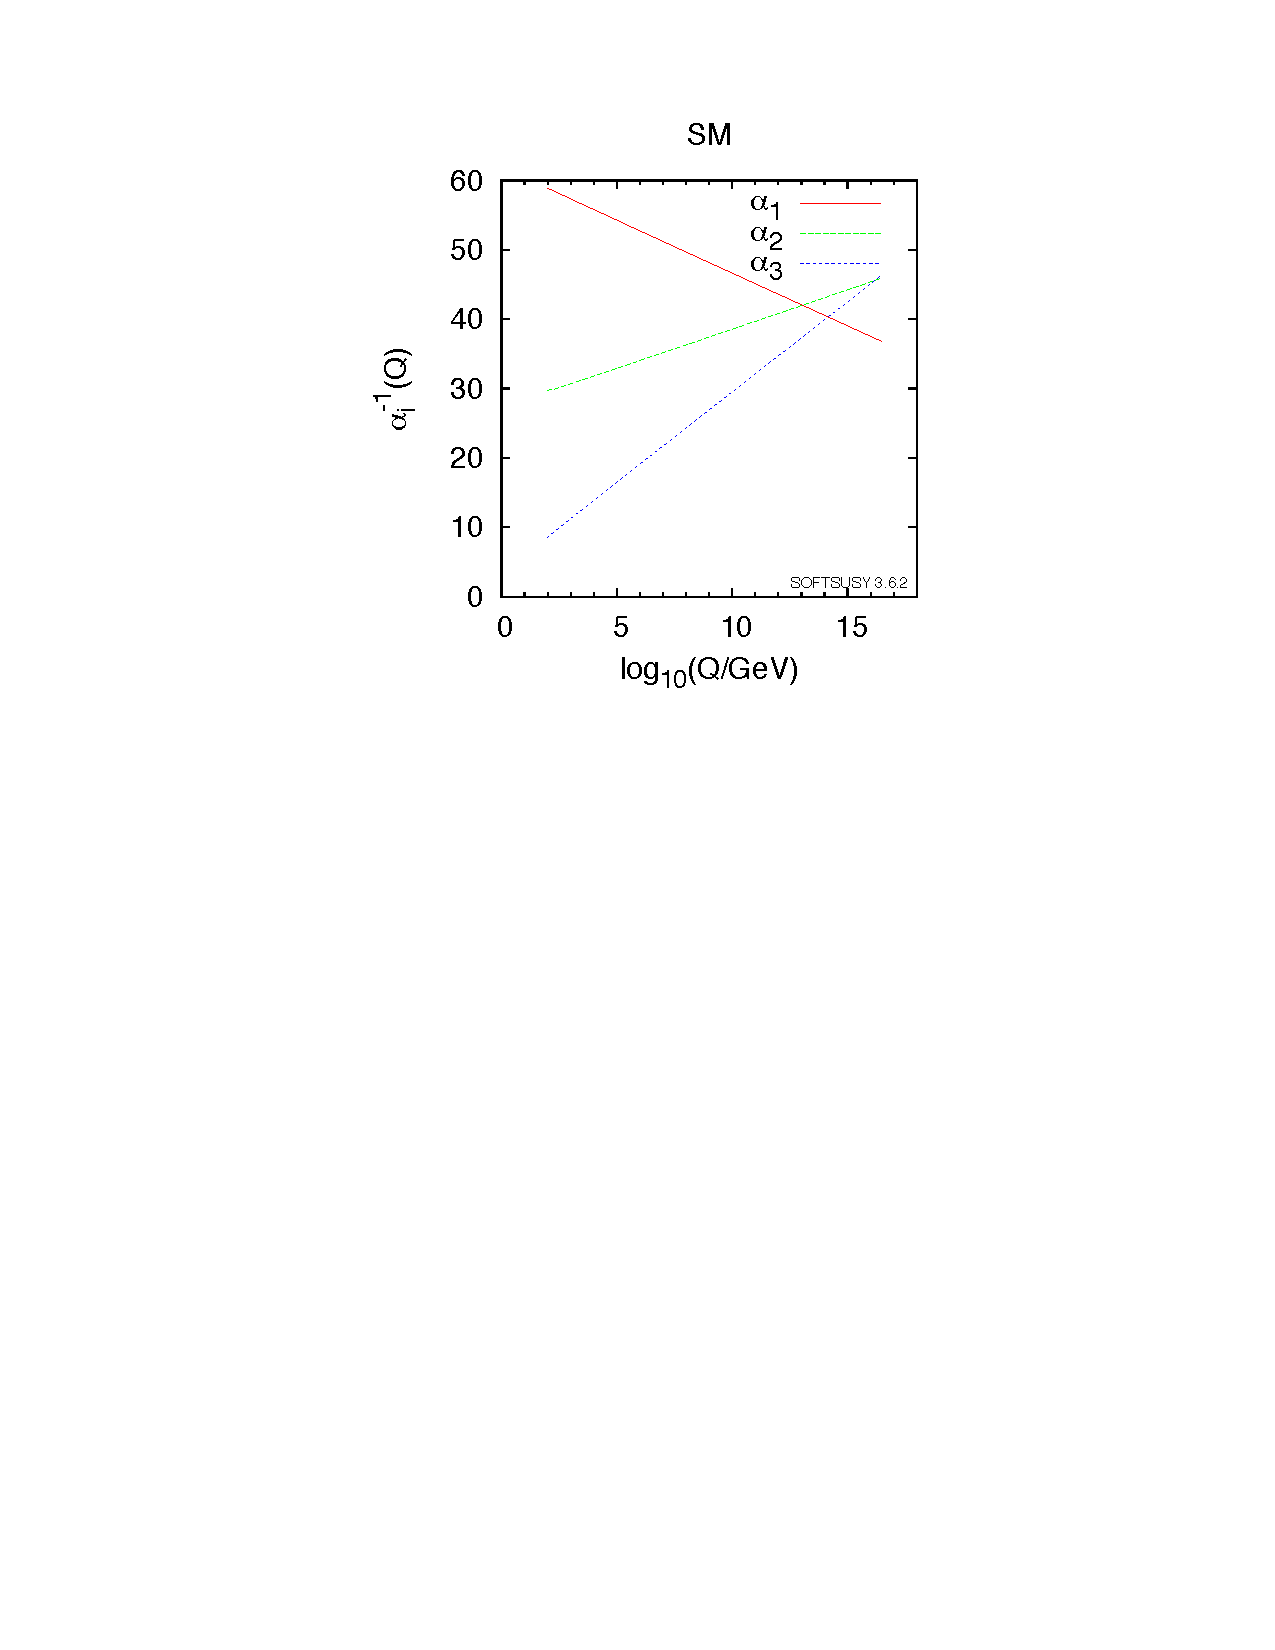
\includegraphics[width=0.49\textwidth]{figures/theory/gut_0.pdf}\label{fig:susy:gut_0}}
\subfigure[]{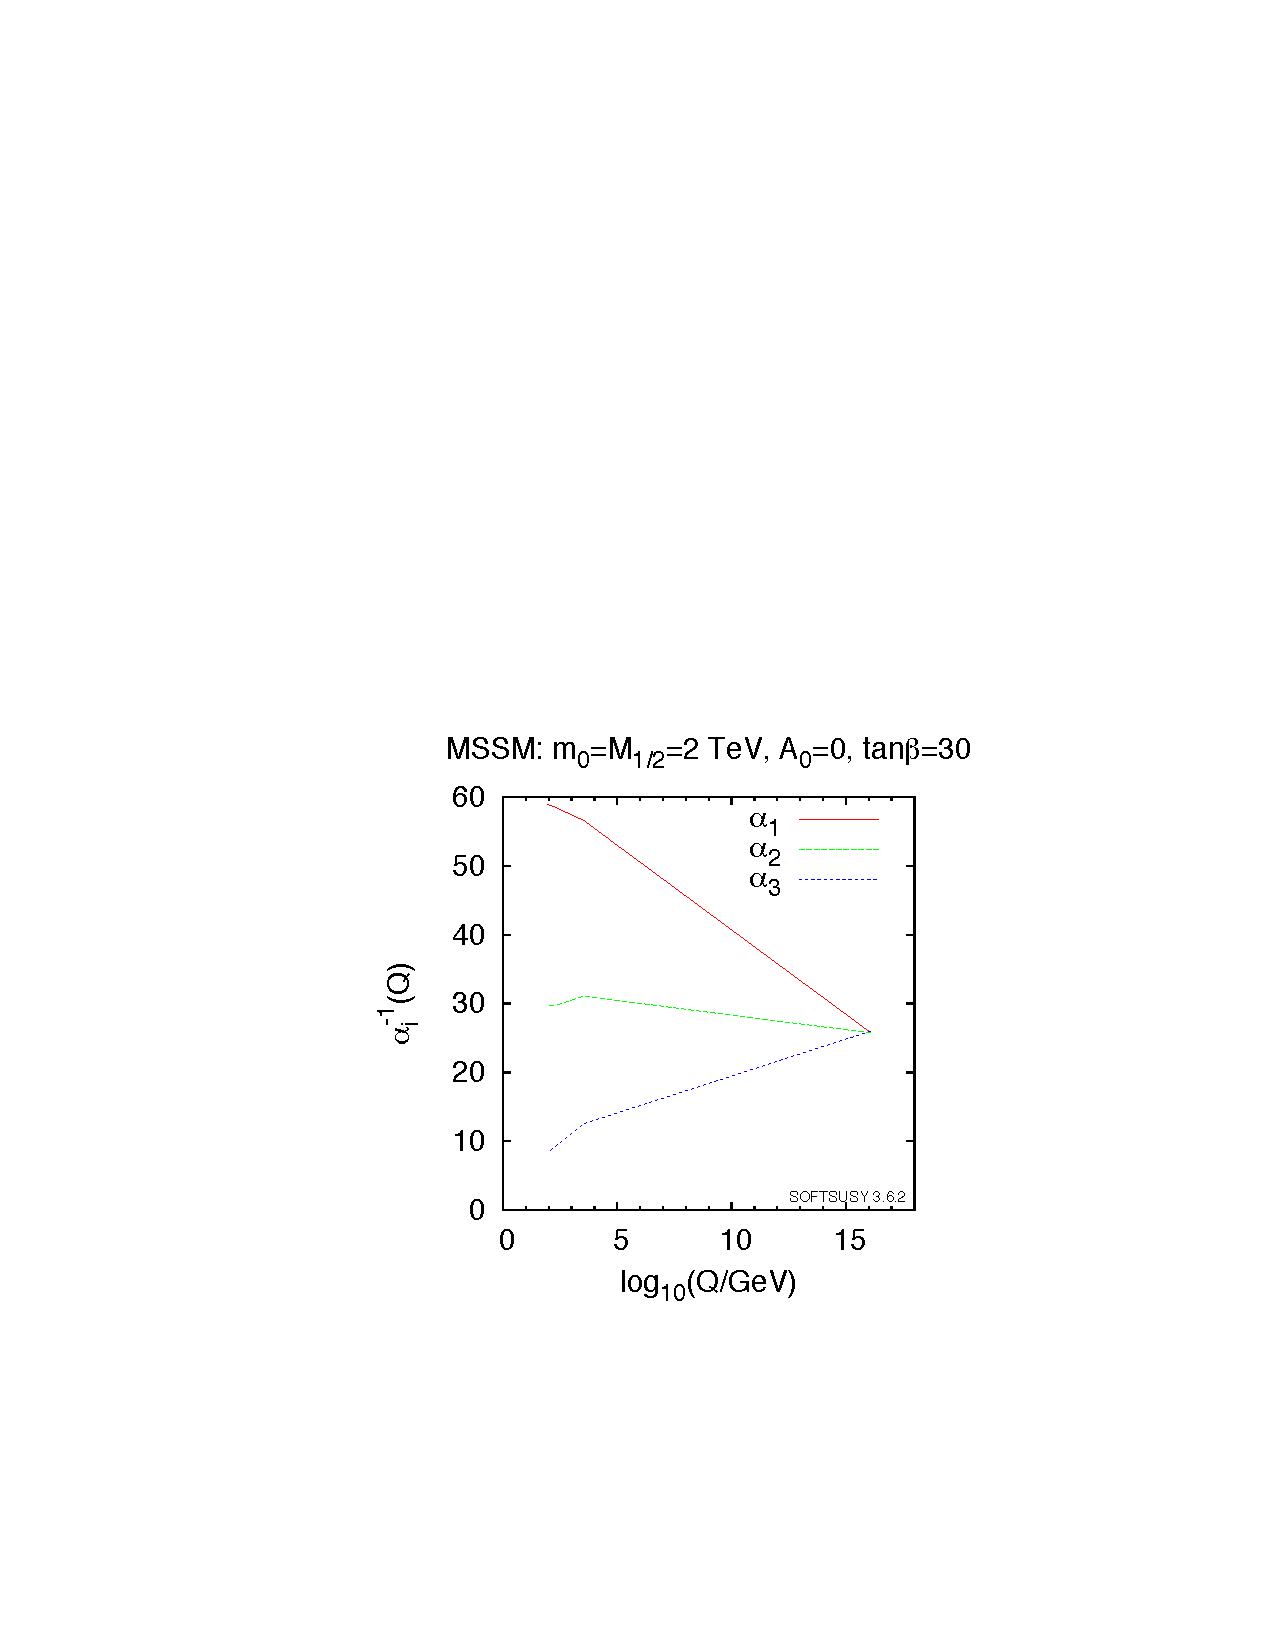
\includegraphics[width=0.49\textwidth]{figures/theory/gut_1.pdf}\label{fig:susy:gut_1}}
\caption{Evolution of the gauge couplings with energy scale in \subref{fig:susy:gut_0} the \gls{sm} and \subref{fig:susy:gut_1} the \gls{mssm}. Figure from Ref. \cite{Patrignani:2016xqp}.}
\label{fig:susy:gut}
\end{figure}

\subsubsection*{MSSM Higgs Sector}
\label{sec:susy:Higgs}

To maintain an holomorphic superpotential, \gls{susy} requires at least two SU(2) doublets: one to give mass to up-type quarks ($H_u$) and one to give mass to the the down-type quarks ($H_d$). The two doublets provide eight degrees of freedom. Three of them are  needed to give masses to the gauge bosons, while the other five become observable particles:
\begin{itemize}
\item Two CP-even neutral Higgs bosons: $h^0$ (the lighter) and $H^0$.
\item $A^0$, a CP-odd Higgs boson.
\item Two charged Higgs bosons, $H^+$ and $H^-$.
\end{itemize}


\subsubsection*{R-parity}

The \gls{mssm} does not include all the possible terms that are gauge- and \gls{susy}-invariant, to avoid interactions that would violate lepton or baryon number conservation. Matter parity, defined as:

\begin{equation}
P_M = (-1)^{3 (B-L)} \; ,
\label{eq:defmatterparity}
\end{equation}

\noindent is a multiplicative quantum number whose conservation implies automatically the conservation of lepton and baryon numbers (denoted with $L$ and $B$ respectively), without having to impose their conservation by hand. Particles in the same supermultiplet have the same matter parity: $P_M =-1$ for lepton and quark supermultiplets, while the Higgs and gauge supermultiplets have $P_M =+1$.

A more convenient way to express the same conservation rule is R-parity:

\begin{equation}
P_R = (-1)^{3(B-L) + 2 s} \; ,
\label{eq:defRparity}
\end{equation}

\noindent where $s$ is the spin of the particle. This is equivalent to matter parity as $(-1)^{2s}$ is conserved in all interactions where angular momentum conservation holds. The advantage of R-parity over matter parity is that for all \gls{sm} particles $P_R = 1$ and for all \gls{susy} particles $P_R=-1$. If  R-parity is conserved, in a collider experiment \gls{susy} particles are always produced in pairs, and each \gls{susy} particle always has an odd number of \gls{susy} particles in its decay products. As a consequence, the \gls{lsp} is stable; if the \gls{lsp} is electrically neutral, it interacts with ordinary matter mainly through gravity and thus it provides a good candidate for dark matter.

Note that R-parity conservation is not deduced from the theory and thus, while its consequences are appealing (especially the provision of a dark matter candidate), it is not an assumption that holds in all \gls{susy} models.



\subsection{Natural SUSY}
\label{sec:theo:naturalsusy}

Particles within the same supermultiplet share the same electric charge, isospin and \gls{qcd} color as $Q$ and $Q^\dagger$ commute with the generator of the gauge transformations.
The third equality in Equation \ref{eq:susyalgth} implies that $[ (P^\mu)^2 , Q  ]=0$. If we think of this as an operator applied to a supermultiplet, this implies that all the particles within the same supermultiplet should also have the same mass. The superpartners also bring a radiative correction to the Higgs boson mass, since they couple to the Higgs boson with the same coupling constant as their \gls{sm} partners ($y_S=y_f=y$). If we consider the case of a fermion and a sfermion, according to Eqs. \ref{eq:divhf}-\ref{eq:divhs} the two contributions have opposite sign and the total correction is:

\begin{equation}
\Delta m_H^2 \>=\> {y\over 16 \pi^2}
\left [ m_f^2
\> {\rm ln}(\Lambda_{UV}/m_f) 
- m_S^2
\> {\rm ln}(\Lambda_{UV}/m_S) 
\right ].
\label{eq:divhsusy}
\end{equation}

This correction cancels if each \gls{sm} particle and its superpartner have the same mass. Unfortunately we know that, if \gls{susy} exists, it must be a broken symmetry as the superpartners do not have the same mass as the corresponding \gls{sm} particles (otherwise they would have been already observed). Since the correction to the Higgs boson mass becomes larger with the increase of the mass difference between particles in the same supermultiplet, \gls{susy} remains a solution to the hierarchy problem as long as this mass difference is reasonably small. The term natural \gls{susy} refers to the class of \gls{susy} models that allow to solve (or mitigate) the fine-tuning problem that affects the Higgs boson mass; this has been a very active topic of discussion both before the start of the \gls{lhc} (see e.g. Refs. \cite{BARBIERI198863, Dimopoulos:1995mi}) and after (e.g. Refs. \cite{Papucci:2011wy, Casas:2014eca}) 

Not all the superpartners have the same relevance in the contribution to the Higgs-mass corrections, and a \gls{susy} model can be natural even if  most particles in it are extremely heavy. The particles that should be light in a natural \gls{susy} model are summarized in Figure  \ref{fig:NaturalSpectrum} and are:
\begin{itemize}
\item higgsinos, whose tree-level mass is directly controlled by the $\mu$ parameter,
\item Stops, which contribute at one loop to the Higgs boson mass, and
\item Gluinos, which contribute at two loops, since they give a one-loop correction to the stop mass.
\end{itemize}

% formula for relation between mass difference and correction to Higgs boson mass

%In the MSSM, the mass of the $Z$ boson and the Higgs sector masses are related at tree level through:
%\begin{equation}
%\label{eq:tune}
%-\frac{m_Z^2}{2} = |\mu|^2 + m_{H_u}^2.
%\end{equation}
%Where $\mu$ is the higgsino mass parameter and $m_{H_u}$ the mass term for the Higgs field that gives mass to down-type quarks. While \ref{eq:tune} holds only at tree level, it still means that if the masses of the superpartners in the Higgs sector are too large, fine-tuned loop corrections will be required to bring the left side of the equation down to the observed value of the $Z$-boson mass.

%\begin{equation}
%\Delta \equiv \frac{2\delta m_{H}^{2}}{m_{h}^{2}}.
%\end{equation}
% Z mass at tree level and definition of fine tuning

% susy particles that have to be light 

\begin{figure}[h!]
\begin{center} 
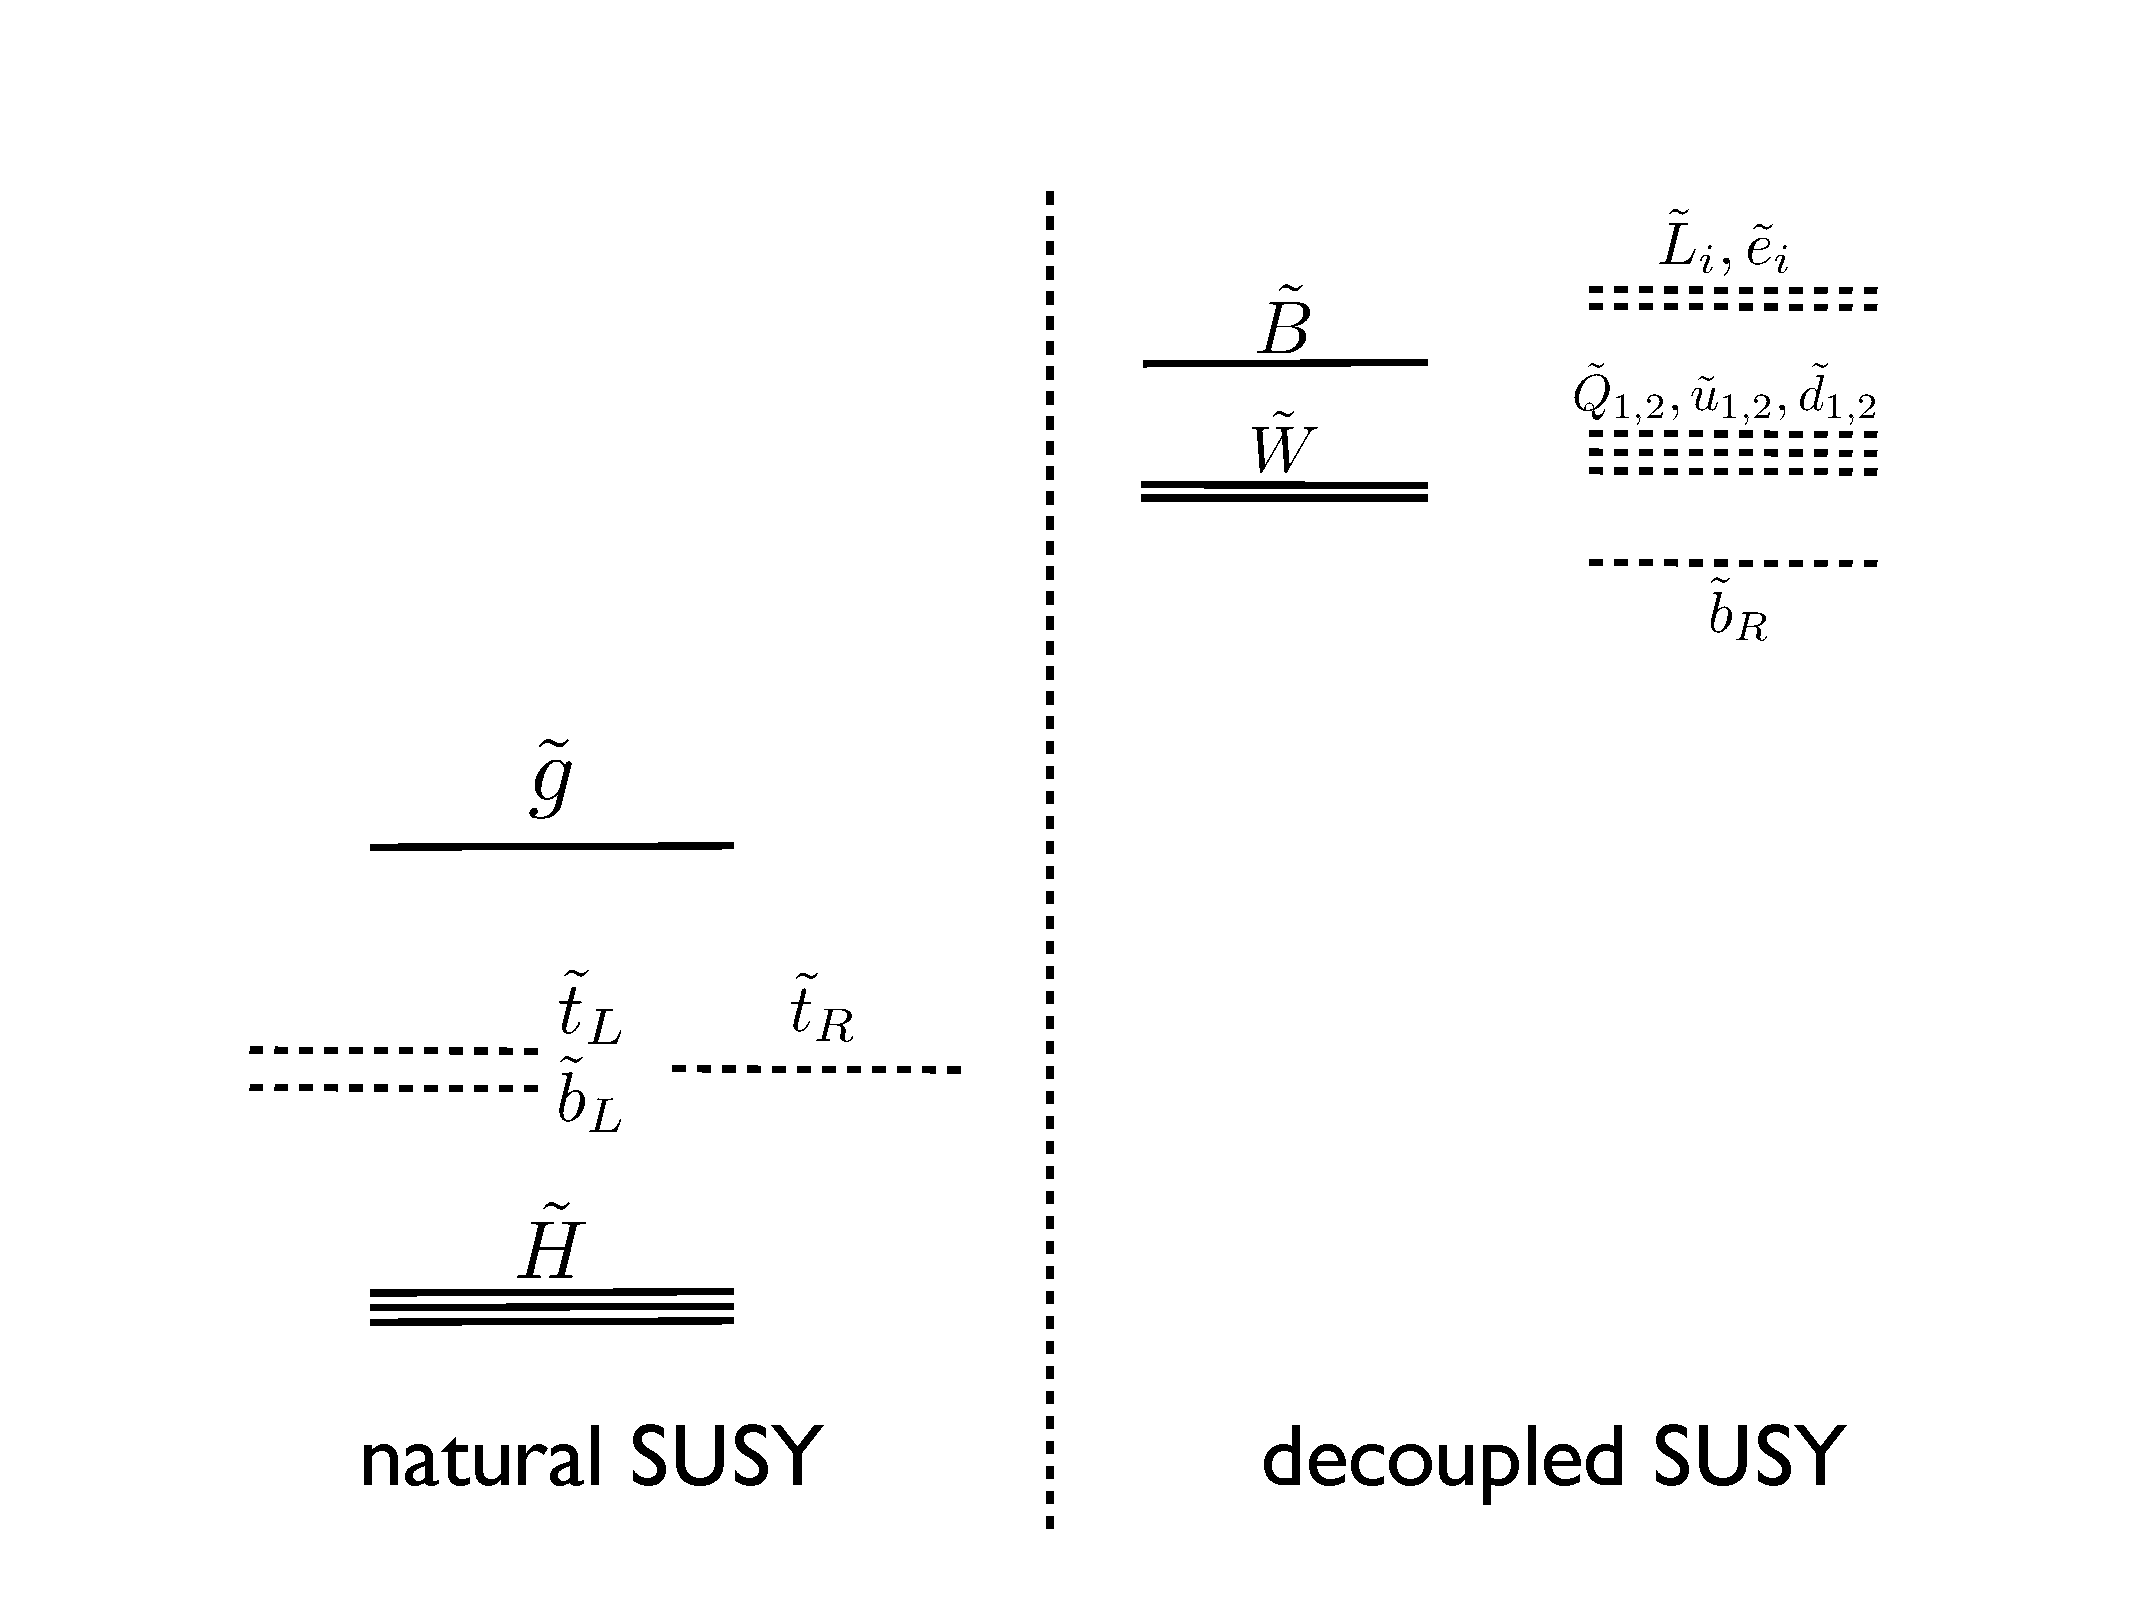
\includegraphics[width=0.9\textwidth]{figures/theory/NaturalSpec.pdf} 
\end{center}
\caption{The Naturalness argument constrains the masses of the \gls{susy} particles on the left side of the figure to be light, while the superpartners on the right side of the figure can have arbitrary mass without spoiling the Naturalness of the model. Figure from Ref. \cite{Papucci:2011wy}.}
\label{fig:NaturalSpectrum}
\end{figure}


\subsection{SUSY breaking in the MSSM}

Superpartners of the \gls{sm} particles have not been observed yet. This means that, if they exist, their mass must be larger than that of the corresponding \gls{sm} particle, and thus \gls{susy} must be a broken symmetry. The Lagrangian can therefore be written as:

\begin{equation}
\lagr = \lagr_{\rm SUSY} + \lagr_{\rm soft} \; ,
\end{equation}

\noindent where $\lagr_{\rm SUSY}$ is the \gls{susy}-conserving part derived from the superpotential, while $\lagr_{\rm soft}$ encloses the terms that break \gls{susy}. The suffix "soft" means that we allow in the Lagrangian only soft \gls{susy}-breaking terms, whose couplings have positive mass dimension, so that they vanish at very high mass scales. The inclusion of \gls{susy}-breaking terms requires the addition of new particles and interactions to the \gls{mssm}. While there is no unambiguous way to modify the theory to do this (some examples of \gls{susy}-breaking mechanisms are described in Section \ref{sec:susybreaking}), it is possible to include in the Lagrangian a general parametric form of the \gls{susy}-breaking terms:
\begin{itemize}
\item Gaugino masses, which in the \gls{mssm} correspond to the bino, wino and gluino mass terms;
\item Non-holomorphic scalar squared masses, which add mass terms for squarks and sleptons and contribute to the Higgs potential;
\item Holomorphic scalar squared masses, that in the \gls{mssm} can be present only in a term like $b H_u H_d$;
\item Scalar cubic couplings.
\end{itemize}  

The necessary \gls{susy}-breaking part of the Lagrangian adds to the \gls{mssm} many free parameters: in total the \gls{mssm} has 105 parameters in addition to the \gls{sm} ones.


\subsection{SUSY-breaking mechanisms}
\label{sec:susybreaking}

The \gls{susy}-breaking terms of $\lagr_{\rm soft}$ can be generated in models where \gls{susy} is spontaneously broken. This is the case if, just like  for the electroweak symmetry breaking, the Lagrangian is \gls{susy}-invariant, but the vacuum state is not. As it happens with the Higgs mechanism, the spontaneous breaking of a symmetry implies the appearance of a massless Goldstone particle (goldstino, $\stilde{G}$) that, in the case of \gls{susy}, has to be a neutral Weyl fermion in order to have the same quantum numbers as the supercharge $Q$. To be massless and annihilate the fermion mass matrix, the goldstino field has to be proportional to:

\begin{equation}
 \stilde{G} \,=\, 
 \begin{pmatrix}
\langle D^a \rangle /\sqrt{2} \cr \langle F_i\rangle 
\end{pmatrix} \; ,
\label{explicitgoldstino}
\end{equation} 

\noindent where $D^a$ and $F_i$ are respectively the auxiliary real bosonic and complex fermion fields of the \gls{susy} Lagrangian, and $\langle \rangle $ denotes their vacuum expectation value. For Equation \ref{explicitgoldstino} to be non-trivial, at least one of the $D^a$ or $F_i$ has to have a non-zero \gls{vev}. This is related to the two possible mechanisms that lead to \gls{susy} breaking: via a $D$-term or an $F$-term. 
The Fayet-Iliopoulos mechanism \cite{Fayet:1974jb} allows to have a non-zero \gls{vev} for an auxiliary field $D$ by adding to the Lagrangian a term proportional to the auxiliary field itself, and with a coupling constant with the dimension of a squared mass:
\begin{equation}
\lagr_{\rm FI} \,=\, -\kappa D \; .
\end{equation}
With this mechanism it is however difficult to attribute properly masses to all the \gls{mssm} particles.
%This type of term is gauge-invariant only for abelian groups. 
%the hypercharge symmetry group $U(1)_Y$ is not eligible 

Another possibility is to assign a \gls{vev} to an $F$-term, with the O’Raifeartaigh mechanism \cite{ORaifeartaigh:1975nky}. Since in the \gls{mssm} there is not a good candidate to be a gauge singlet with a non-vanishing \gls{vev} for an $F$-term, this implies the addition of at least one set of chiral supermultiplets, such that $F_i$ is non-trivial for at least one of them. A realization of this is possible for example with three chiral supermupliplets $\Phi_i$ and a superpotential of the form:
\begin{equation}
W = -k \Phi_1 + m \Phi_2 \Phi_3 + {y\over 2} \Phi_1 \Phi_3^2 \;.
\label{oraif}
\end{equation}
The resulting scalar potential at tree level has a minimum for $\phi_2=\phi_3=0$ and independent of $\phi_1$ (where $\phi_i$ are the scalar fields in $\Phi_i$), while the one-loop corrections highlight a non-zero global minimum when also $\phi_1=0$. In the following we will consider only \gls{susy} breaking originating from the O’Raifeartaigh mechanism.


When \gls{susy} is treated as a local symmetry, it has to include also gravity, and the resulting theory is called supergravity. The gravity mediator is the spin-2 graviton, and its superpartner the spin-$\frac{3}{2}$ gravitino. The gravitino can be interpreted as the gauge field of \gls{susy}, and it incorporates the goldstino degrees of freedom upon spontaneous \gls{susy} breaking. Therefore, the gravitino is also indicated with the same symbol as the goldstino, $\stilde{G}$. By dimensional arguments, we can understand that the gravitino mass ($m_{3/2}$) has to be proportional to:

\begin{equation}
m_{3/2} \approx \frac{\langle F \rangle}{\Lambda_P} \; ,
\label{mgrav}
\end{equation}
\noindent where $\langle F \rangle$ is the \gls{vev} of the \gls{susy}-breaking $F$-term, as it has to vanish both if \gls{susy} is an exact symmetry and if the Planck scale is extremely high (and thus gravity is negligible). 

For any \gls{susy}-breaking mechanism, the \gls{mssm} soft term do not appear at tree level, but are generated through radiative corrections. \gls{susy} breaking happens in a hidden sector, while the \gls{mssm} particle live in the visible sector, and experiment the consequences of the spontaneous \gls{susy} breaking happening in the hidden sector through interactions that couple both sectors. Depending on which interaction is driving the communication between the \gls{susy}-breaking sector and the \gls{mssm}, we can distinguish three main mechanisms:

\subsubsection*{PMSB} 

If supergravity and the other new physics effects that arise at the Planck scale are the responsible of the connection of the hidden sector with the \gls{mssm} sector, then the order of magnitude of the soft parameters in the \gls{mssm} is:
\begin{equation}
m_{\rm{soft}} \approx \frac{\langle F \rangle}{\Lambda_P} \; .
\label{msoft_PMSB}
\end{equation}
\noindent This ratio is motivated by the observation that $m_{soft}$ should vanish both in the limit where \gls{susy} is an exact symmetry, as well as in the limit where the Planck mass is very large and the interactions mediated by gravity are not anymore sizable. We refer to this scenario as \gls{pmsb} \cite{PhysRevLett.49.970, BARBIERI1982343, IBANEZ198273, PhysRevD.27.2359}. In \gls{pmsb} models, the gravitino mass has the same order of magnitude as the mass of the other superpartners (as we can notice by comparing Equation~\ref{mgrav} and Equation~\ref{msoft_PMSB}), and therefore it can not be particularly light. 

\subsubsection*{AMSB}

If the supregravity couplings that mediate \gls{susy} breaking in \gls{pmsb} models are absent, \gls{susy} can be broken through loop effects. In \gls{amsb} models \cite{Randall:1998uk,Giudice:1998xp} scalar and gaugino masses are generated through one-loop corrections arising from superconformal anomalies. These corrections are always present, but are dominant only in models that do not include tree-level terms. In the simplest \gls{amsb} model leads to the prediction of negative squared masses for sfermions; one possible extension to the model that solves this problem is the addition of a scalar mass parameter $m_0^2$, common to all scalar squared masses. 

\subsubsection*{GMSB}

In the case of \gls{gmsb} \cite{Dine:1981gu, AlvarezGaume:1981wy, Nappi:1982hm, PhysRevD.48.1277, Dine:1994vc, Dine:1995ag} the interactions mediating the connection between the hidden sector and the \gls{mssm} are the same gauge interactions of the \gls{mssm} itself. This requires to add to the theory a set of chiral supermultiplets (mediators) that interact both with the source of supersymmetry breaking and with the \gls{mssm} particles (through loop corrections to their masses, involving the \gls{mssm} gauge interactions). The mediators contribute at one loop to the mass of gauginos, while they have a two-loop contribution to the mass of squarks and leptons. In both cases, the mass scale of the superpartners is:
\begin{equation}
m_{\rm{soft}} \approx \frac{\langle F \rangle}{M_\mathrm{mediator}} \; .
\label{msoft_GMSB}
\end{equation}
\gls{sm} gauge bosons are not affected by the loop corrections induced by the mediators as their mass is protected by the gauge symmetry.
If we compare Equation \ref{msoft_GMSB} with Equation \ref{mgrav} we can see that, as long as the mass of the mediators is lower than the Planck scale, the gravitino can be significantly lighter than the rest of the superpartners. In most \gls{gmsb} models the gravitino is the \gls{lsp}, and all particles decay to it. While we could expect the decay rate to a $\stilde{G}$ to be low because of the weakness of the gravitational interaction, this is not the case as the gravitino inherits the gauge interactions of the goldstino it absorbs during the spontaneous supersymmetry breaking.  
\gls{susy} breaking introduces a large number of free parameters with respect to the \gls{sm}.
Most of these new parameters lead to flavor-changing interactions that are highly suppressed experimentally. 
In models of gauge mediation, the interaction between the \gls{susy}-breaking sector and the \gls{mssm} happens only through gauge interaction, that are flavor-blind, and therefore the suppression of flavor-changing effects is implemented automatically.



\subsection{Phenomenological MSSM}
\label{sec:theory:pmssm}

The \gls{pmssm} \cite{Djouadi:1998di} reduces the number of free parameters in the \gls{mssm} through some assumptions motivated by experimental evidence. In particular:
\begin{itemize}
\item To avoid flavor changing neutral currents, the sfermion mass matrices and all the trilinear couplings are diagonal. 
\item The presence of CP-violating terms is bound to be only the one predicted by the \gls{sm} by imposing that all the new parameters are real numbers.
\item The first two generations of sfermions are degenerate i.e. the corresponding elements in the first and second generation have the same mass, to circumvent existing limits on the splitting between the first ans second squark generations.
\item Since the trilinear couplings give rise to amplitudes that are proportional to the corresponding Yukawa coupling, only the third generation ones are relevant and the others are set to zero.
\end{itemize}

These assumptions allow to reduce the number of free parameters from 105 to 19 (summarized in Table \ref{tab:pMMSpar}), making phenomenological analyses possible.


\begin{table}[h]
\centering
\begin{tabular}{c c}
\hline 
Parameter & Description \\ 
\hline 
\hline
$M_1, M_2  \, M_3 $ & Gaugino mass parameters \\ 
\hline 
$\tan \beta$ & Ratio of the \glspl{vev} of the two Higgs doublets \\ 
\hline 
$M_A$ & Pseudoscalar Higgs boson mass parameter \\ 
\hline 
$\mu$ & higgsino mass parameter \\ 
\hline 
$  A_t, \, A_b, \, A_\tau    $ & Third generation trlinear couplings \\ 
\hline 
$m_{qL},  \,  m_{uR},  \, m_{dR},  m_{lL},  \, m_{eR}$ & First (and second) generation sfermion masses \\ 
\hline 
 $m_{q3L}, \, m_{tR}, \, m_{bR}, \, m_{\stilde{L}}, \, m_{\stilde{\tau}_R},$ & Third generation sfermion masses \\ 
\hline 
\end{tabular} 
\caption[Free parameters of the \gls{pmssm}]{\label{tab:pMMSpar}List of free parameters in the \gls{pmssm}.}
\end{table}





% Supersymmetry (SUSY) is a \gls{bsm} framework that allows to generate an infinite amount of \gls{bsm} models, each with different signatures.

%\chapter{LHC and ATLAS}
\label{chap:cern}

The analyses presented in this thesis use the data collected by the ATLAS experiment in 2015, 2016 and 2017 at \cmtre TeV; the ATLAS experiment is one of the four main experiments at the Large Hadron Collider (LHC) at CERN. Section \ref{sed:cern:lhc} of this chapter describes the LHC accelerator complex, followed by a description of the ATLAS detector in Section \ref{sed:cern:atlas}.

%%%%%%%%%%%%%%%%%% LHC

\section{The Large Hadron Collider}
\label{sed:cern:lhc}

In this section we give a brief introduction to the Large Hadron Collider (LHC) \cite{1748-0221-3-08-S08001}, at the moment the largest and most powerful particle accelerator in the world, hosted by the European Organization for Nuclear Research (CERN) and active since September 2008.



\subsection{A Circular Hadron Collider}

The LHC is a circular hadron accelerator, located in a 26.7-km-long underground tunnel (with a depth ranging between 50 and 140 meters) that was previously hosting the Large Electron-Positron Collider (LEP), a CERN accelerator active from 1989 to 2000. The LHC can accelerate protons up to a design center-of-mass energy of 7 TeV. Accelerating particles to very high energies is necessary to both study the structure of the particles themselves at smaller scales, and to create heavy states in collisions. Cosmic rays provide a source of particles with energies up to $10^7$ times more than what the LHC is capable of, but these extremely energetic rays are very rare, and the flux is not controlled. Accelerators provide a well controlled flux of particles of a specific type in a specific location, and this allows the study of these particles with dedicated detectors.

A circular accelerator simplifies the acceleration of the particles, as this can happen over several revolutions. When a charged particle travels on an orbit of radius r under the effect of a magnetic field B, its momentum p is given by:
\begin{equation}
\label{eq:cern:p03br}
p = 0.3 B r,
\end{equation}
\noindent where the momentum is expressed in GeV, B in Tesla and the radius of the orbit in meters. For a given magnetic field, a larger radius allows to reach higher energies. 

The choice of a collider over a fixed-target experiment is motivated by the possibility of reaching an higher energy in the center of mass system: while in a fixed-target experiment this is proportional to the square root of the incoming particle, in a collider is the sum of the energies of the two beams.


Suitable particles for a collider experiment need to fulfill two criteria: they need to be charged, in order to be accelerated and guided through electric and magnetic fields, and they need to be stable enough not to decay before being used for collisions. These criteria effectively limit the choice to protons, electrons and their antiparticles, in addition to ions. 

At the LHC it has been chosen to study collisions with protons and lead ions. Three types of collisions are studied: proton-proton ($p-p$), lead-lead ($Pb-Pb$) and also proton-lead ($Pb-p$). The main reason to prefer protons over electrons is the energy loss that affects charged particles accelerated in a circular trajectory (\textit{syncrotron radiation}), that decreases with the fourth power of the mass of the particle:

\begin{equation}
\label{eq:cern:sync}
\frac{dE}{dt} \propto \frac{E^4}{m^4 r}
\end{equation}

The larger mass of a proton with respect to an electron leads to a decrease of a factor $10^{12}$ of the energy lost for syncrotron radiation. This choice comes with a price: proton-proton collisions lead to less clean events, where a lot of soft interactions covering the interesting hard interactions and the center of mass is unknown as the particles taking part in hard interactions are not the protons themselves but their constituents.

\subsection{Magnet System} 


The LHC is not a perfect circumference: it is composed by eight arcs (\textit{sectors}), where the magnetic system is located, and eight straight sections containing the resonant cavities, the detectors, the equipment for beam injection and extraction, and other instrumentation. Magnetic fields are used to govern the trajectory of the particles. In the LHC there are more than nine thousand magnets, constructed from a superconducting alloy of niobium and titanium. 150 tons of super-fluid helium at the temperature of 1.9 K are used to maintain the magnet system in the superconducting regime. The different types of magnets necessary to achieve a proper control over the trajectory of the particles are:

\subsubsection*{Dipoles} 
Dipoles are used to create a vertical magnetic field, to bend the particles in the horizontal plane and give the dominant circular orbit. The LHC has 1232 dipoles, each 15 m long and providing a magnetic field of 8.3 T. The current necessary to achieve this strong magnetic field is 11.8 kA.


\subsubsection*{Quadrupoles}
The LHC has 858 quadrupoles, used for beam focusing. A single quadrupole can focus the beam either in the vertical or horizontal plane, but causes a defocusing on the other; conventionally a quadrupole is denoted as focusing if it is oriented to focus in the horizontal plane. A combination of focusing and defocusing quarupoles separated by some drift space (\textit{FODO lattice}) is used to keep both planes focused, and gives rise to \textit{Betatron oscillations}. Fig. \ref{fig:lhc:quad} shows a schematic representation of the transverse view of a quadrupole magnet.

\subsubsection*{Higher-order Magnets} 
Beside dipoles and quadrupoles, in the LHC there are about 600 higher-order magnets are used to maintain a good beam quality; for example sextupoles are used to correct the spread in Betatron tune caused by the quadrupoles.




\begin{figure}[ht]
\centering
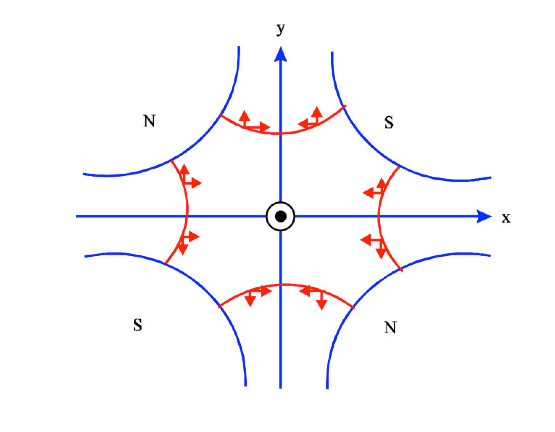
\includegraphics[width=0.45\textwidth]{figures/lhc/figures_quad}
\caption{A schematic cross-section of a quadrupole magnet. The red arrows indicate the direction of the force on the particle. Figure from Ref. \cite{Kain:2016aly}.}
\label{fig:lhc:quad}
\end{figure}

\subsection{Resonant Cavities}

While the orbit of the particles is governed through magnetic fields, longitudinal electric fields are used for acceleration. In the LHC the electric filed is provided by the \textit{radiofrequency (RF) cavities}. There are overall 16 RF cavities, 8 per beam, hosted in four cryo-modules. Each cavity can create a field up to 2 MV (providing an accelerating field of 5 MV/m), and oscillates with a frequency of 400 MHz. Since the electric field changes over time with the oscillations, particles passing through the same point of a RF cavity in different moments experience a different voltage; this produces a non-trivial longitudinal dynamic, where particles oscillates around the ideal synchronous particle with changes is momentum and phase (\textit{Synchrotron oscillations}). If we define the \textit{slip factor} $\eta$ as the relative change in frequency in Synchrotron oscillations with the relative change in momentum:
\begin{equation}
\eta = \frac{\Delta f / f}{\Delta p / p}
\end{equation}

and the compaction factor $\alpha$ as the relative change in frequency in orbit length with the relative change in momentum:

\begin{equation}
\eta = \frac{\Delta L / L}{\Delta p / p} \; ,
\end{equation}

the following relation holds:
\begin{equation}
\eta = \frac{1}{\gamma^2} - \alpha \; ,
\end{equation}

where $\gamma$ is the Lorentz factor of the particle. This means that while the energy of the particle is low ($\eta>0$) an increase in momentum leads to an increase in frequency, while it leads to a decrease in frequency for $\eta<0$. At the transition energy a previously stable synchrotron phase becomes unstable and vice versa; this requires a rapid change in RF phase. This situation is illustrated in Fig. \ref{fig:lhc:phase}(a). For example, a particle corresponding to the phase point M1 will arrive in the RF cavity after one corresponding to the stability point P1, and will experiment higher voltage and increase in momentum; if $\eta>0$ this increase in momentum will translate in an increase in frequency and the particle will, at the following revolution, arrive earlier, while if $\eta<0$ the frequency will further decrease and the particle will be eventually lost.  The transition energy in the LHC is 53 GeV, well below the injection energy of 450 GeV, so the LHC is always above transition. 

\begin{figure}[ht]
\centering
\subfigure{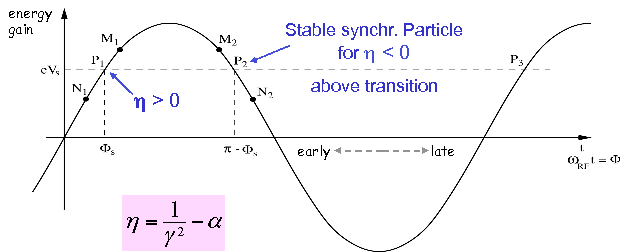
\includegraphics[width=0.547\textwidth]{figures/lhc/phase-stability-2}}
\subfigure{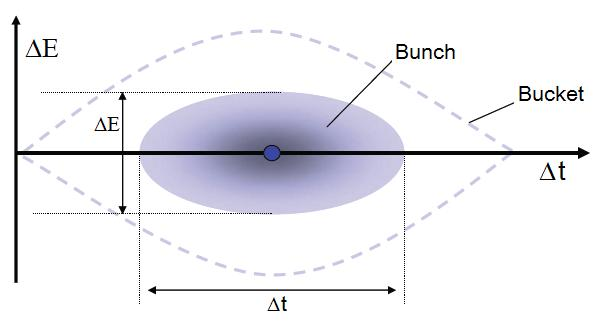
\includegraphics[width=0.44\textwidth]{figures/lhc/bucket}}
\caption{(a) Phase stability below and above transition. Figure from Ref. \cite{Tecker:2016mlq}. (b) Bucket and the bunch area.}
\label{fig:lhc:phase}
\end{figure}


In the LHC beams particles are not distributed continuously, as this would now be allowed by phase instabilities, but are divided in \textit{bunches}. 
The areas of stable motion are identified as \textit{bucket}, and the area of the bucket is the beam \textit{longitudinal acceptance}. The beam bunches fill only a part of the bucket, and the area of the beam bunches is the \textit{longitudinal beam emittance}. Fig. \ref{fig:lhc:phase}(b) shows a schematic view of the bucket and the bunch area.

\subsection{Operational Parameters}

The amount of data collected by an accelerator is quantified by the \textit{integrated luminosity} $\mathcal{L}_{int}$.
Given a certain process with production cross section $\sigma$, the total number of events for that process is the product of cross section and integrated luminosity:

\begin{equation}
\label{eq:cern:nev}
N_{\mathrm{events}} = \sigma \,\, \mathcal{L}_{int} \; .
\end{equation}

The integrated luminosity is the time integral of the \textit{instantaneous luminosity} $\mathcal{L}$, 

\begin{equation}
\label{eq:cern:intlumi}
\mathcal{L}_{int} = \int \mathcal{L} \, dt
\end{equation}

and the instantaneous luminosity is in turn defined as:

\begin{equation}
\mathcal{L}=\frac{f N_b n^2}{4 \pi \sigma_{x,y} } \;
\label{eq:cern:lumi}
\end{equation}

where f is the revolution frequency, $N_b$ the number of bunches in each beam, $n$ the number of protons in each bunch and $\sigma_{x,y}$  is the transverse beam size at the interaction point. The transverse size can be expressed as:

\begin{equation}
\sigma_{x,y} = \sqrt{  \epsilon \beta^* } \; ,
\end{equation}

where $\epsilon$ is the beam emittance and $\beta^*$ the betatron function. The instantaneous luminosity defined in Eq. \ref{eq:cern:lumi} needs to be corrected for two factors. First of all, this formula assumes a head-on collision between the bunches; in reality, to avoid unwanted interactions the beams collide with a crossing angle, and a large crossing angle decreases the instantaneous luminosity.

\begin{table}[ht]
\begin{center}
\begin{tabular}{c c c c c }
\hline 
Parameter & 2015 & 2016 & 2017 & Design \\ 
\hline 
\hline
Prtons per bunch (n) [$10^{11}$ p] & $\approx$ 1.2 & $\approx$ 1.1 & $\approx$ 1.2 & 1.15 \\ 
\hline 
Number of bunches (N$_b$) & 2244 & 2220 & $\approx$ 2250 & 2780 \\ 
\hline 
Emittance ($\epsilon$) [mm mrad] & $\approx$ 3.5 & $\approx$ 2.2 & $\approx$ 2.2 & 3.5 \\ 
\hline 
Betatron function ($\beta^*$) [cm] & 80 & 40 & 40 (33) & 55 \\
\hline
Crossing angle [$\mu$rad] & 290 & 370 (280) & 300 (340) & 285 \\
\hline
Peak luminosity [$10^{34} cm^{-2}s^{-1}$] & 0.51 & 1.4 & 1.7(1.9) & 1.0 \\
\hline
\end{tabular}
\end{center}
\caption{LHC operational parameters in Run2.}
\label{tab:lhc:param}
\end{table}



\subsection{Accelerator Complex}

\begin{itemize}
\item Linac
\item PS Booster
\item PS
\item SPS
\end{itemize}

\begin{figure}[ht]
\centering
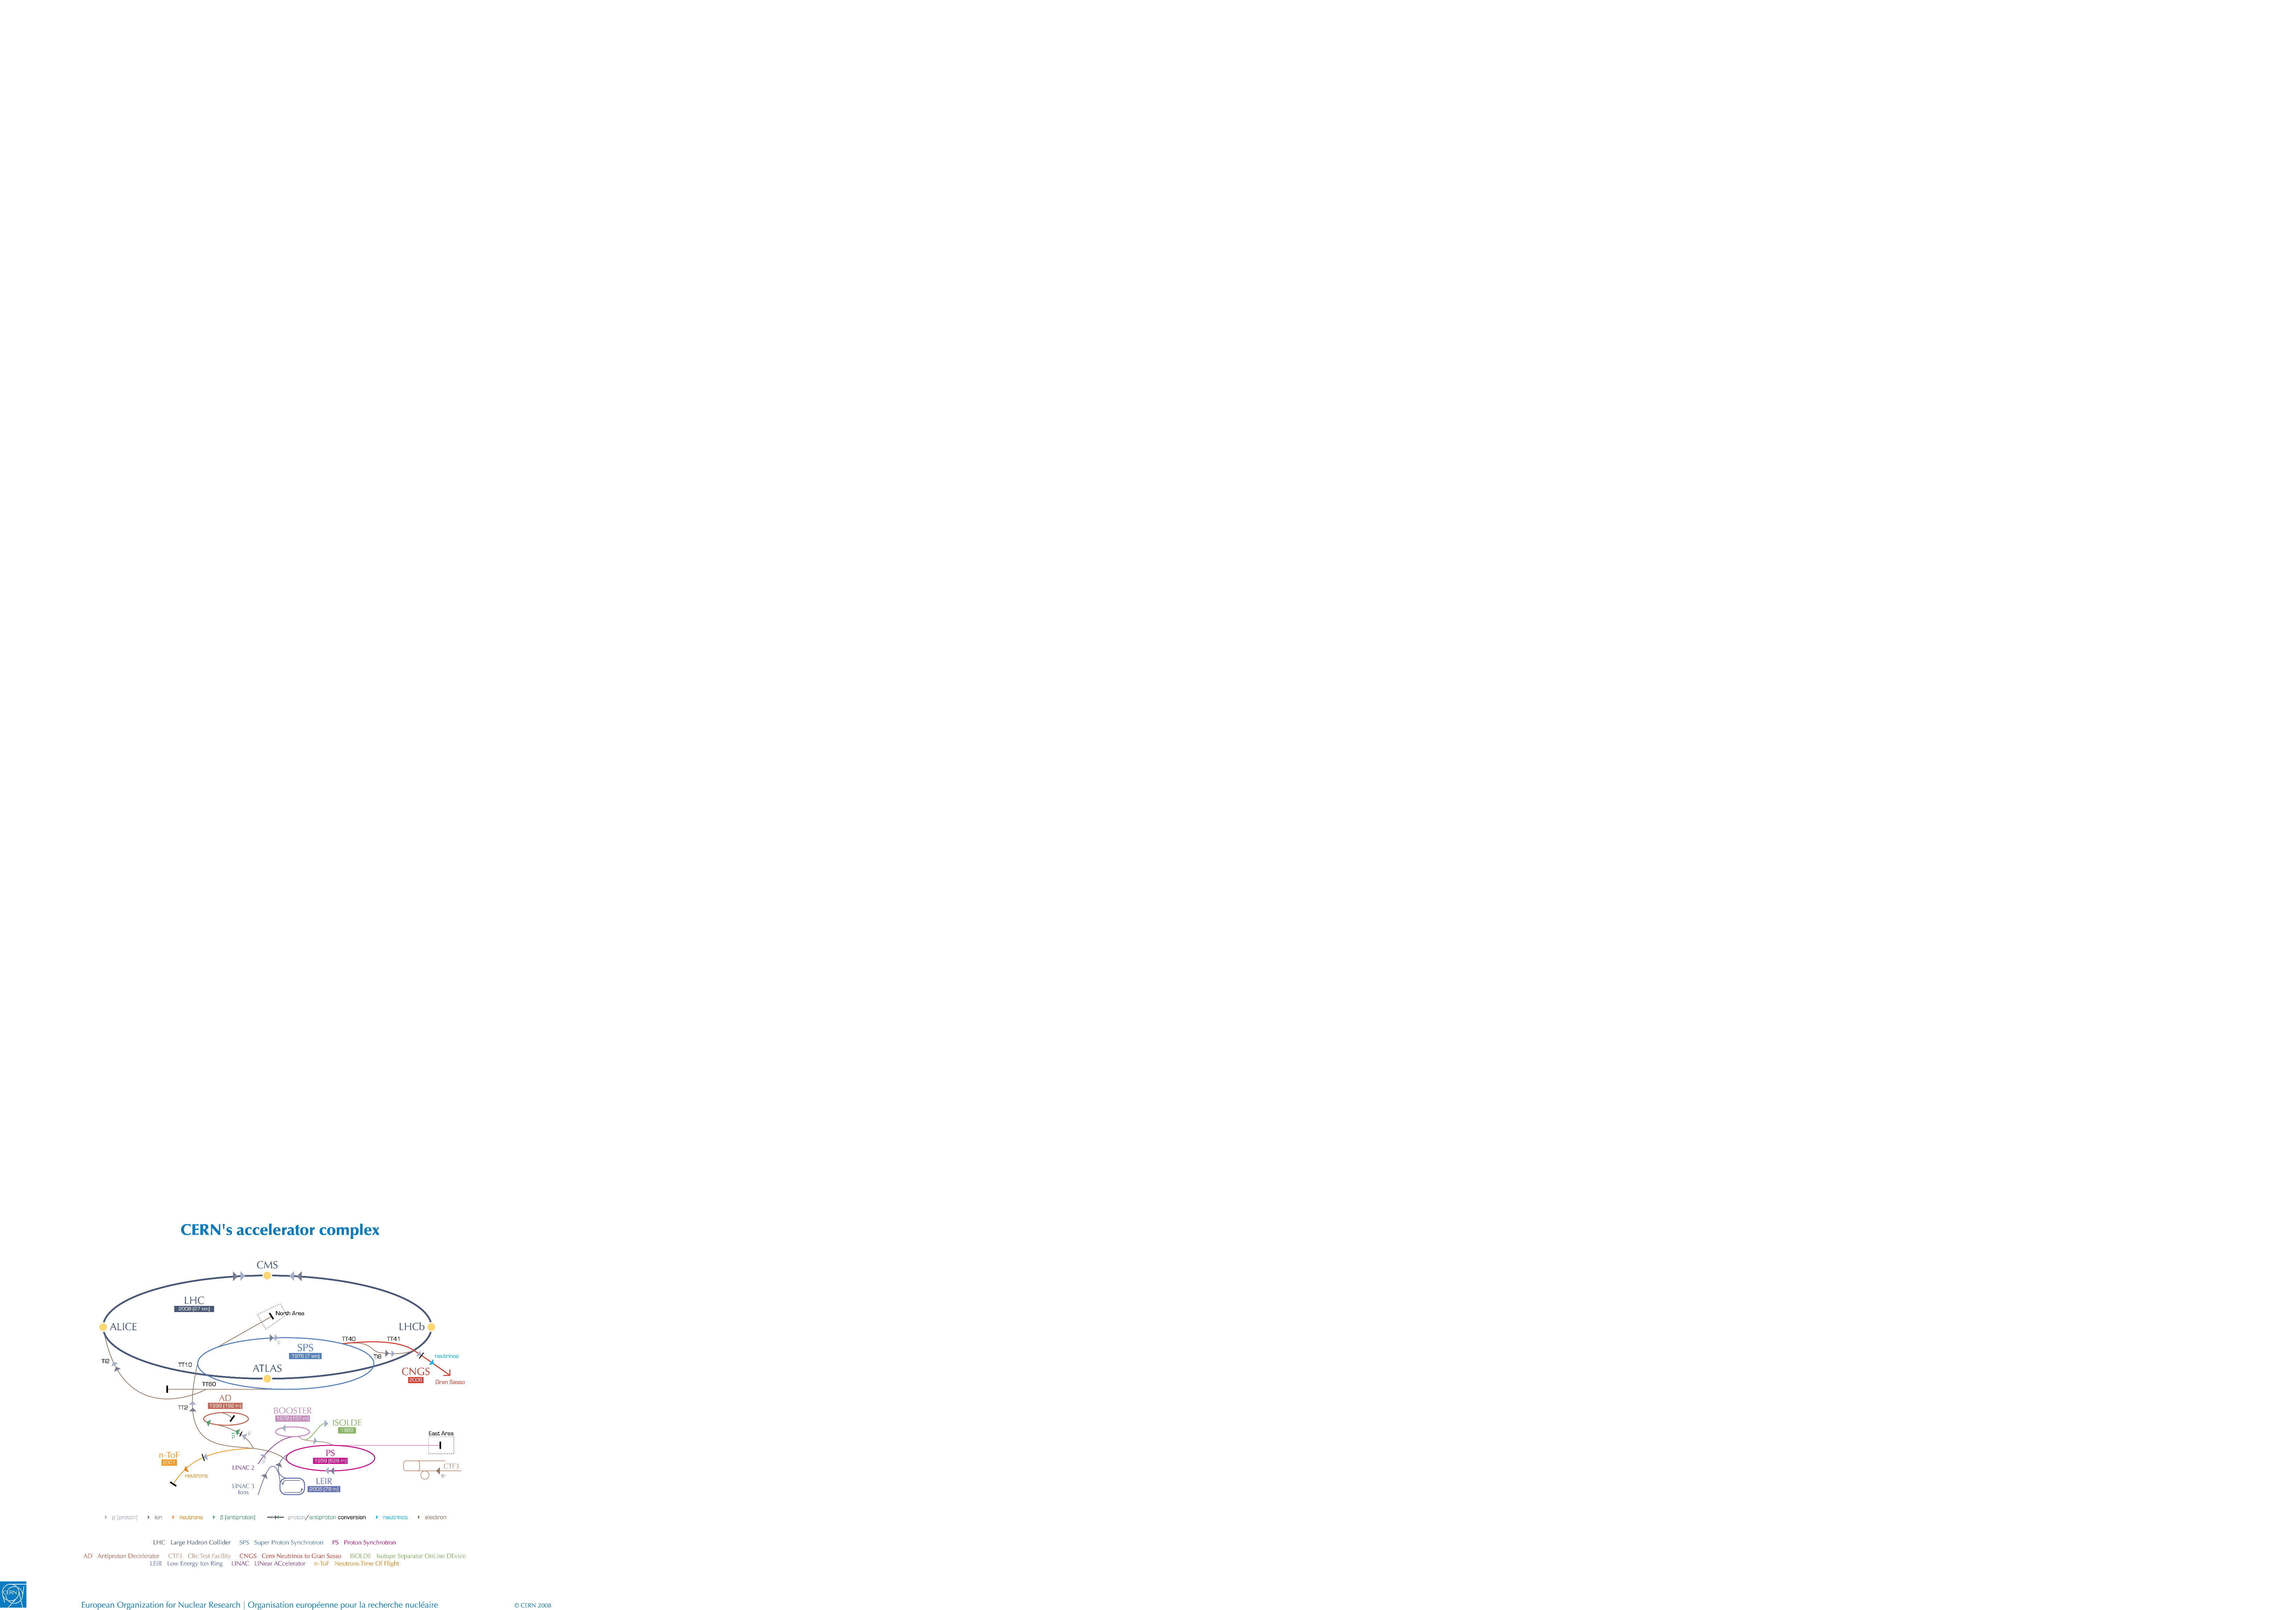
\includegraphics[width=1\textwidth]{figures/lhc/acc_complex.pdf}
\caption{CERN accelerator complex \cite{Christiane:1260465}.}
\label{fig:lhc:acc}
\end{figure}

\subsection{Experiments at the LHC}

\subsubsection*{ALICE}

\subsubsection*{CMS}

\subsubsection*{LHCb}

\subsubsection*{LHCf}

\subsubsection*{TOTEM}

\subsubsection*{ALICE}

\subsubsection*{MoEDAL}


%%%%%%%%%%%%%%%%%% ATLAS

\section{The ATLAS Experiment}
\label{sed:cern:atlas}

\subsection{Coordinate System}

\begin{equation}
\label{eq:cern:eta}
\eta = - \ln \tan \frac{\theta}{2}
\end{equation}

\begin{equation}
\label{eq:cern:y}
y = \frac{1}{2} \ln \frac{E + p_z}{E - p_z}
\end{equation}

\begin{equation}
\label{eq:cern:pt}
p_T = \sqrt{p_x^2 + p_y^2}
\end{equation}

\begin{equation}
\label{eq:cern:pz}
p_z = p_T \,\sinh \eta
\end{equation}

\begin{equation}
\label{eq:cern:dR}
\Delta R = \sqrt{ \Delta \phi^2 + \Delta \eta^2  }
\end{equation}




\subsection{Magnet System}
\label{sec:cern:atlasmagnets}

\subsubsection*{Solenoid}

\subsubsection*{Toroids}



\subsection{Inner Detector}

\subsubsection*{IBL}

\subsubsection*{Pixel Detector}


\subsubsection*{Semi-Conductor Tracker}


\subsubsection*{Transition Radiation Tracker}



\subsection{Calorimeters}

\subsubsection*{Electromagnetic Calorimeter}


\subsubsection*{Hadronic Calorimeter}


\subsubsection*{Forward Calorimeter}


\subsection{Muon Spectrometer}


\subsection{Forward Detectors}

\subsection{Trigger System}
\label{sec:cern:trigger}

\subsection{ATLAS Performance Summary}


\subsection{ATLAS Physics Program}
%\chapter{Physics Objects Reconstruction}
\label{sec:event:reco}

The particles produced in the \gls{pp} collisions in the center of the \gls{atlas} detector, interact with the detector material as discussed in Chapter \ref{chap:cern}. As a result of these interactions, electrical currents are recorded. \textit{Event reconstruction} is the process of recombining these digital signals and interpreting them as tracks and energy deposits in the calorimeters. A further step consists in analyzing the characteristics of the candidate tracks and calorimeter clusters and identify them as signs of the passage of specific particles.
This chapter describes the reconstruction and identification of the objects used in the analyses discussed in this thesis: tracks and vertices, electrons, muons, hadronic jets and missing transverse momentum. 


\section{Tracks and Primary Vertices}
\label{sec:reco:tracks}

In \gls{atlas} the identification of tracks from charged particles relies on the information collected by the \gls{id}. The tracking information is crucial to the reconstruction and identification of many types of particles, including electrons, muons, and the jest originating from the hadronization of a b-quark. The precision on the position measurement of the track depends on the granularity of the different subsystems of the \gls{id} and, since the \gls{id} is surrounded by a solenoidal magnetic field, the charged particles follow an helical trajectory. After the point of closest approach (perigee) to a given reference is defined, the trajectory of the track can be described by five parameters: 
\begin{equation}
\theta, \; \phi, \; q/p \; d_0, \; z_0 \;,
\end{equation}
\noindent where $\theta$ and $\phi$ are the azimuthal and polar angle, $q/p$ is the ratio of the charge of the track to the track momentum, and $d_0$ and $z_0$ are the distance to the point of closest approach in the transverse plane and along the $z$-axis. 

Primary tracks, originating from charged particles with a life time longer that $3 \times 10^{-11}$ s produced directly in the hard-scatttering vertex, are reconstructed with an inside-out approach \cite{Cornelissen:1020106}: the seed of the reconstruction are three hits in the silicon detector, and then compatible hits in the outer layers of the \gls{id} are added with a Kalman Filter \cite{citeulike:347166,Fruhwirth:1987fm}. The \gls{trt} segments that are not associated with primary tracks are used as starting point to reconstruct tracks from long-lived particles or from material interaction, with a back-tracking that extrapolates the \gls{trt} information to the pixel hits. 

Random groups of hits can be wrongly reconstructed as belonging to the helical trajectory of a track (\textit{fake tracks}). The amount of fake tracks increases with the increase of pile-up, and can be reduced by tightening the selection criteria of the track, at the expense of reconstruction efficiency. Three different selection criteria are used for the data collected in 2015 and 2016 (Loose, Loose-Primary and Tight-Primary), that differ in the requirements on the hits and holes (elements where a hit was expected but was not registered) in the different \gls{id} layers. The \textit{track reconstruction efficiency} is measured in \gls{mc} simulations as the ratio of the reconstructed tracks matched to a generated charged particle over the total number of generated charged particles. The reconstruction efficiency as a function of the track $\eta$ and \pt is shown in Fig. \ref{fig:obj:tracks} for Loose and Tight-Primary tracks.
 
\begin{figure}[ht]
\centering
\subfigure[]{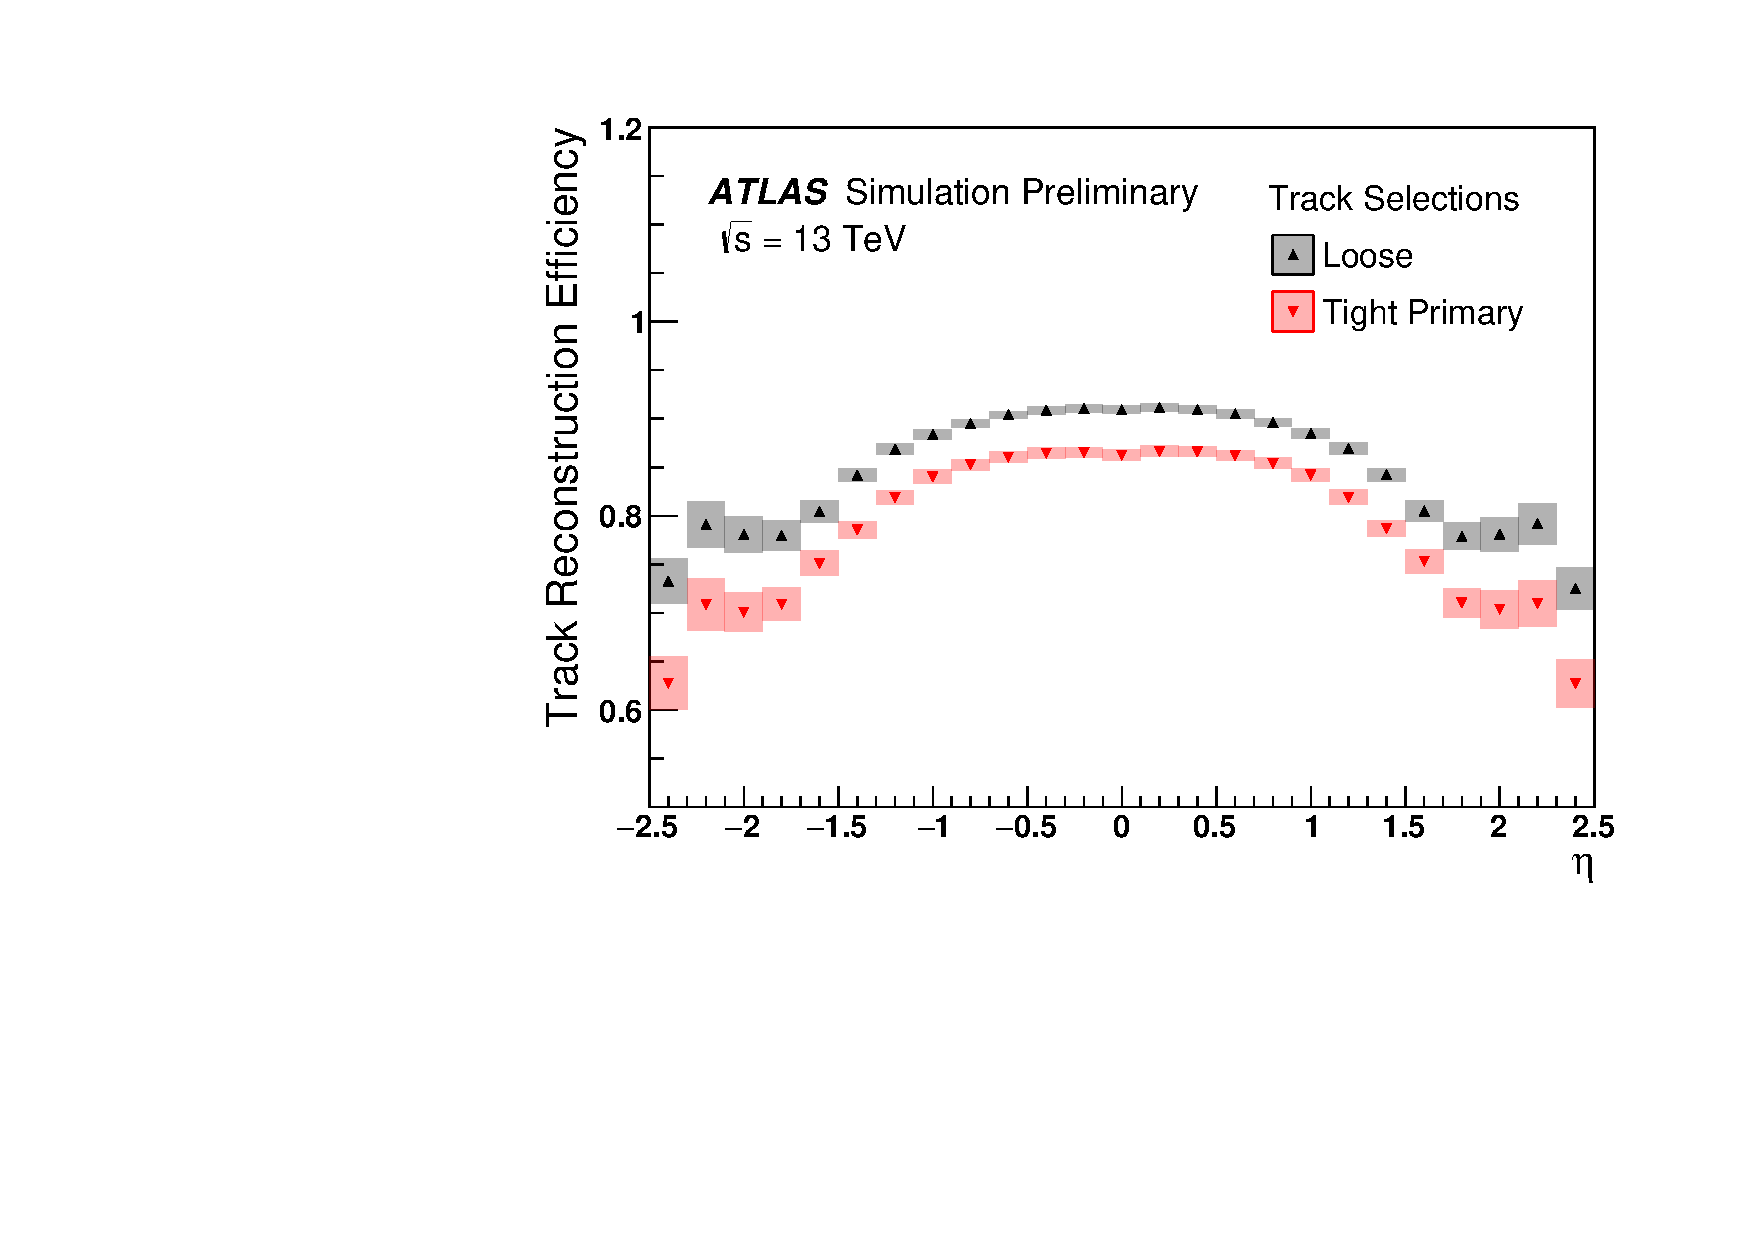
\includegraphics[width=0.48\textwidth]{figures/objects/track1}}
\subfigure[]{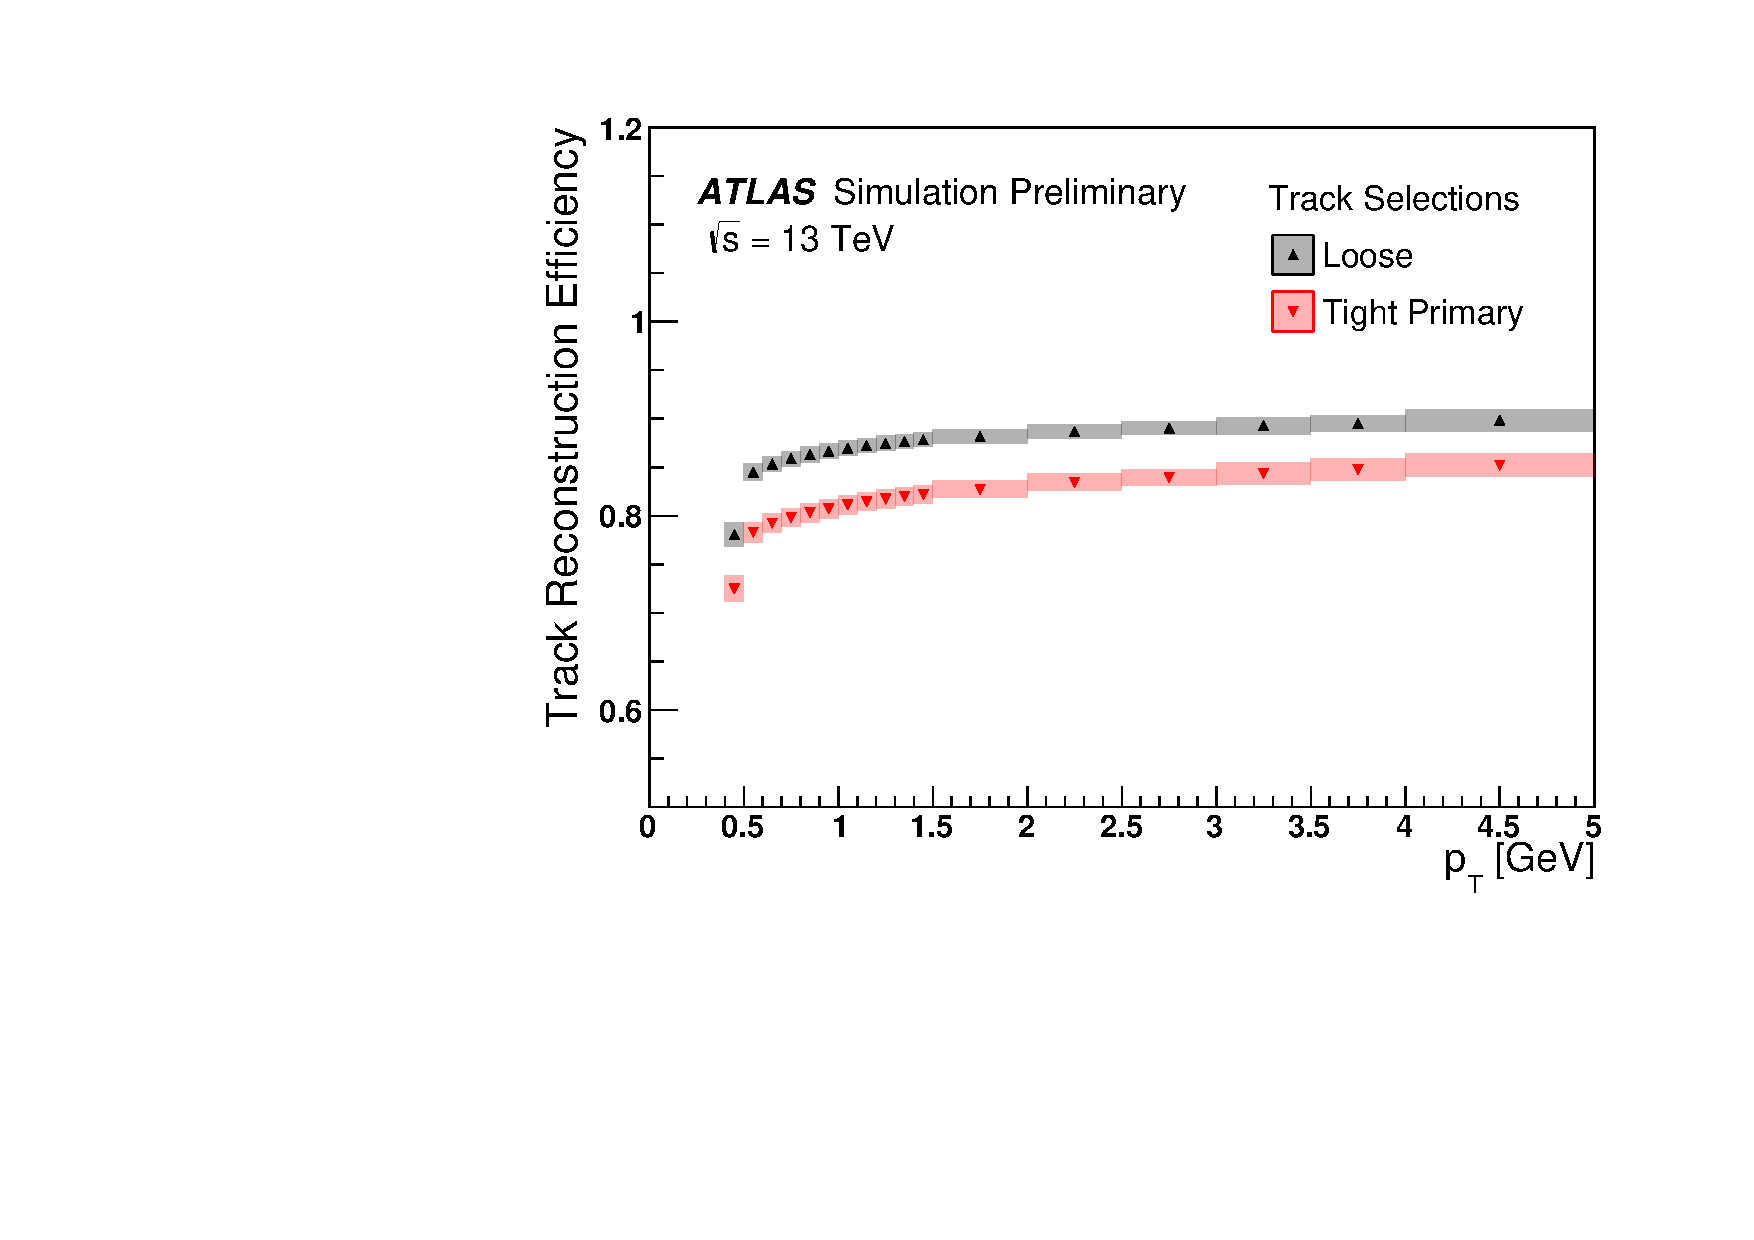
\includegraphics[width=0.48\textwidth]{figures/objects/track2}}
\caption{Track reconstruction efficiency, evaluated by using minimum bias simulated events, as a function of truth $\eta$ (a) and \pt (b) for Loose and Tight Primary track selections.The bands indicate the total sstematic uncertainty. Figure from Ref. \cite{ATL-PHYS-PUB-2015-051}.}
\label{fig:obj:tracks}
\end{figure}

Tracks are the starting point for the identification of vertices. \glspl{pv} are reconstructed through a vertex fitting algorithm \cite{Fruhwirth:2007hz}, and then the vertex fitting algorithm identifies the vertex position and refits the tracks adding the constraint of the reconstructed interaction point. Once all the \glspl{pv} are reconstructed, the one with the highest sum of the squared transverse momenta of its associated tracks ($\sum_i^{N-tracks}p_{T,i}^2$) is identified as the hard scattering vertex, and $d_0$ and $z_0$ are recomputed with respect to its coordinates. The other vertices are named pile-up vertices, and their number is correlated  to the number of interactions per bunch crossing.


\section{Hadronic Jets}

Because of confinement, quarks and gluons produced in the collisions give origin to a collimated spray of hadrons (\textit{jets}) that move in the direction of the original parton. When jets interact with the detector, they loose most of their energy as deposits in the calorimeter systems, which are then grouped together aiming at reconstructing the characteristics of the original parton. 

\subsection{Clusters}
The first step in the jet reconstruction is the procedure that groups the calorimeter cells into topological clusters (\textit{topoclusters}) \cite{Lampl:2008zz,Aad:2016upy}. Topoclusters are built starting from seed cells with a signal-to-noise ratio higher than 4. All the neighboring cells with signal-to-noise ratio higher than two are added with an iterative procedure, and finally a ring of guard cells are added independently of their signal. This procedure is illustrated in Fig. \ref{fig:obj:topocluster}. Topoclusters are calibrated at the \gls{em} scale, which means that the proportionality constant between the readout current and the particle energy is correct only for particles of an \gls{em} shower.

\begin{figure}[h]
\begin{center}
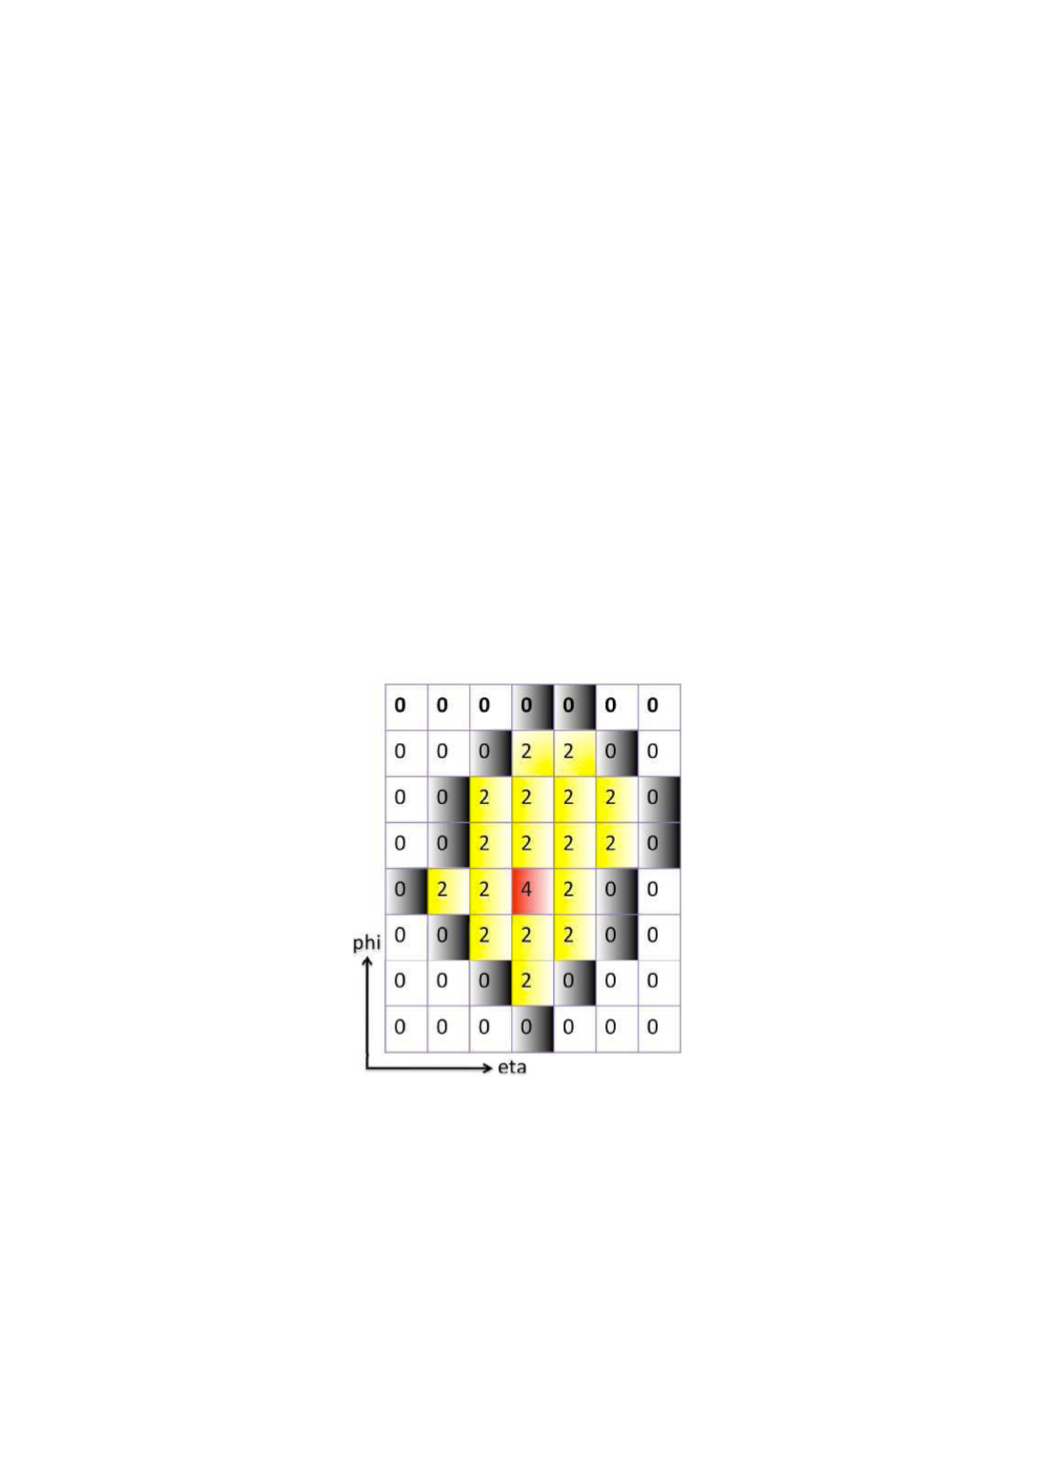
\includegraphics[width=0.3\textwidth]{./figures/objects/topocluster.pdf}
\end{center}
\caption[Topocluster schematic representation]{Topocluster schematic representation. The seed of the cluster is shown in red, the neighbouring cells are in yellow and the ring of guard cells is in grey.}
\label{fig:obj:topocluster}
\end{figure}
 
\subsection{Jet-finding Algorithms}
\label{sec:obj:jetfinding}

The topoclusters are then grouped together by a jet-finding algorithm. Different algorithm are available, and in particular the algorithms of the $k_T$-family merge clusters according to the metric $d_{i,j}$, defined as:

\begin{equation}
d_{i,j} = min\left( k_{T,i}^{2n}, k_{T,i}^{2n}  \right) \frac{\Delta R_{i,j}^2}{R^2},
\label{eq:obj:dij}
\end{equation}

where $k_{T,i}$ is the transverse momentum of the cluster, $\Delta R_{i,j}$ is the angular distance defined as in \ref{eq:deltaR}, $R$ is a fixed parameter, whose values sets the size of the jet, and $n$ is the parameters that defines the kind of algorithm we are using and therefore the shape of the resulting jets. Eq. \ref{eq:obj:dij} defined the distance between two clusters, while the cluster-beam distance is defined as:

\begin{equation}
d_{i,B} =  k_{T,i}^{2n} \; .
\end{equation}

The grouping of the clusters follows an iterative approach:
\begin{enumerate}
\item For each topocluster, the distances $d_{i,j}$ and $d_{i,B}$ are calculated.
\item If, for some $i$ and $j$, $d_{i,j} < d_{i,B}$, group together the two clusters with the smallest $d_{i,j}$
\item Otherwise, if $d_{i,B} < d_{i,j} \, \forall i \neq j $ the $i$-th cluster is defined as a jet.
\item This procedure is iterated until the jet is defined
\end{enumerate}

Depending on the value of the parameter n, we can distinguish different algorithms:
\begin{itemize}
\item $n=0$: Cambridge-Aachen. The grouping of the clusters depends only on geometrical considerations and not on their momentum. 
\item $n=1$: $k_T$ algorithm. Soft clusters are grouped first.
\item $n=-1$: anti-$k_T$ algorithm. Groups hard objects first; the shape of the jets is more regular than in the two previous cases and is a cone of radius R.
\end{itemize}

The choice of a particular algorithm results in different shapes of the jets, represented in fig. \ref{fig:jetsalg}. The standard algorithm used by \gls{atlas} is the anti-$k_T$ algorithm \cite{cacciari:antikt}.

\begin{figure}[h]
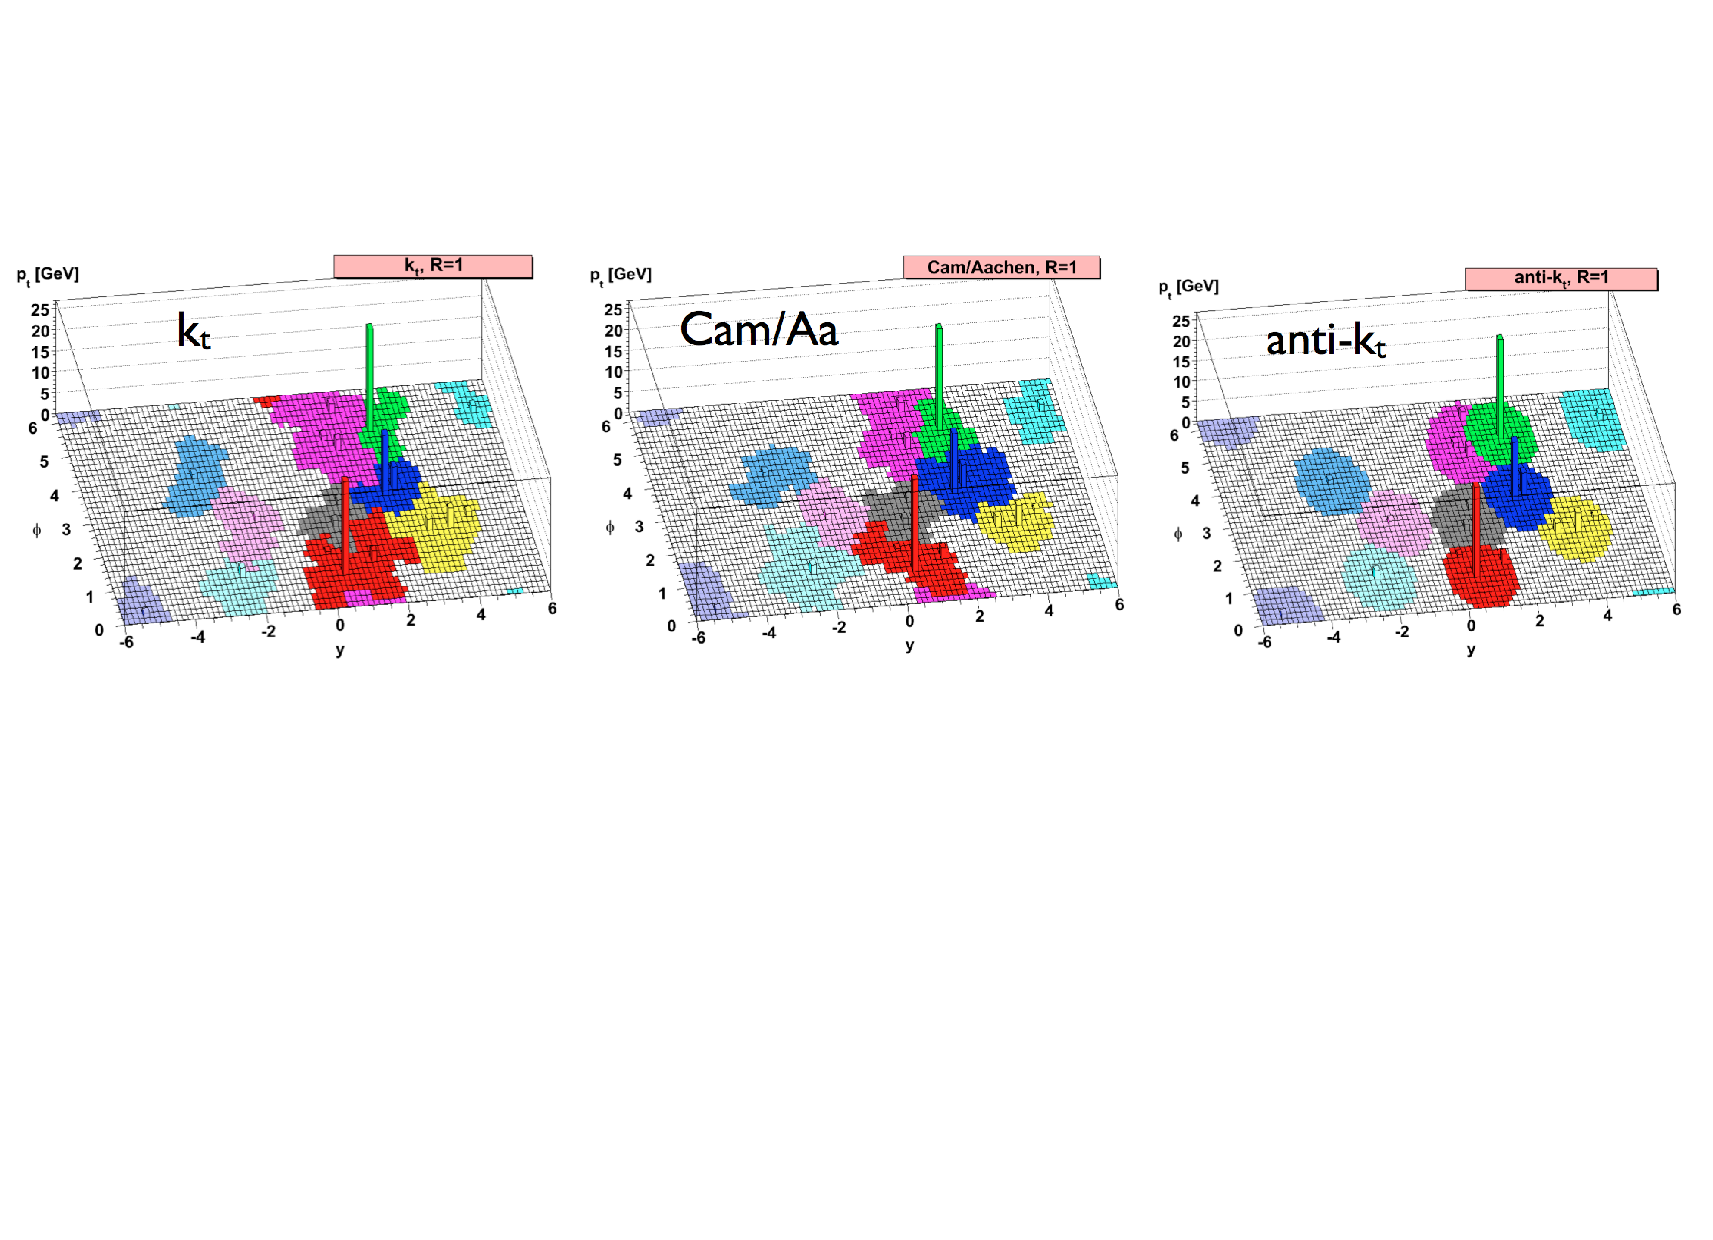
\includegraphics[width=\textwidth]{./figures/objects/jetsalg.pdf}
\caption[Shape of jets reconstructed with different algorithms]{Shape of jets reconstructed with different algorithms \cite{cacciari:antikt}.}
\label{fig:jetsalg}
\end{figure}

\subsection{Jet Calibration}
\label{sec:obj:jetcalib}

As mentioned above, the inputs to the jet-finding algorithms are calibrated at \gls{em} scale, and its coordinate refer to the center of the detector. To access a more precise measurement of the jet energy and kinematics, a sequence of calibration stages are applied; for the 2015-2016 dataset, the standard \gls{atlas} corrections are \cite{PhysRevD.96.072002}:

\begin{description}
\item[Origin correction] The direction of the jet is changed to point at the reconstructed hard-scattering \gls{pv} rather than at the cented of the detector. This correction improves the $\eta$ resolution of the jets.

\item[Pileup correction] Multiple collisions in the same bunch crossing (\textit{in-time pile-up}), as well as residual energy from previous collisions (\textit{out-of-time pile-up}), affect the e jet energy reconstruction. The effect of pile-up is corrected in two steps: a first correction \cite{Cacciari:2007fd,TheATLAScollaboration:2013pia}, dependent on the number of \glspl{pv}, uses the jet area to subtract form the jet energy the average energy form pile-up events. A second correction based on the number of \glspl{pv} and on the number of interactions per bunch crossing, is then applied to disentangle the the effect of in-time pile-uo and out-of-time pile-up.

\item[Absolute calibration] The absolute \gls{jes} and $\eta$ correction is derived comparing in \gls{mc} the truth energy of a jet with the reconstructed energy, and also correct for biases in the $\eta$ reconstruction \cite{Aad2015jets}.

\item[Global sequential calibration] The \gls{gsc} \cite{ATLAS:2015oia} improves the \gls{jes} resolution by deriving additional corrections based on individual jet properties, for example the number of associated tracks and the fraction of energy deposited in the various layers of the calorimeter.

\item[In-situ calibration] As a last stage, the data-driven calibration (\textit{in-situ}) \cite{ATLAS:2015uwa} corrects for the differences between \gls{mc} simulation and data (arising for example from imperfect simulation of the detector response and material interaction). These corrections are derived from events where the jet \pt is balanced against other well measured objects. In the $\eta$-intercalibration, dijet events are used to correct the response of forward jets using well-measured central jets. The response of central jets is instead measured in $Z$+jets, $\gamma$+jets and multijet events. 
 
\end{description}

\subsubsection{Jet Calibration Uncertainties}

The calibration procedure described above implies a set of uncertainties. In particular, 
the \gls{atlas} \gls{jes} Run-2 calibration includes a set of 80 systematic uncertainties; 
67 of those derive from the in-situ calibration \cite{PhysRevD.96.072002}, accounting for modelling uncertainties, 
sample statistics and uncertainties on the calibration of other physics objects used in deriving the calibration. 
The other 13 systematic uncertainties derive from the pileup correction, the $\eta$-intercalibration 
and differences in the jet response and composition for jets of different flavors. 
The full combination of the uncertainties derived from the first 3.2 \ifb of the Run 2 data 
is shown in Fig. \ref{fig:obj:jessyst} as a function of \pt at $\eta = 0$ and as a function of $\eta$ at \pt$ = 80$ GeV.

\begin{figure}[h]
\begin{center}
  \subfigure[]{
    \label{fig:Comb_syst:pt}
    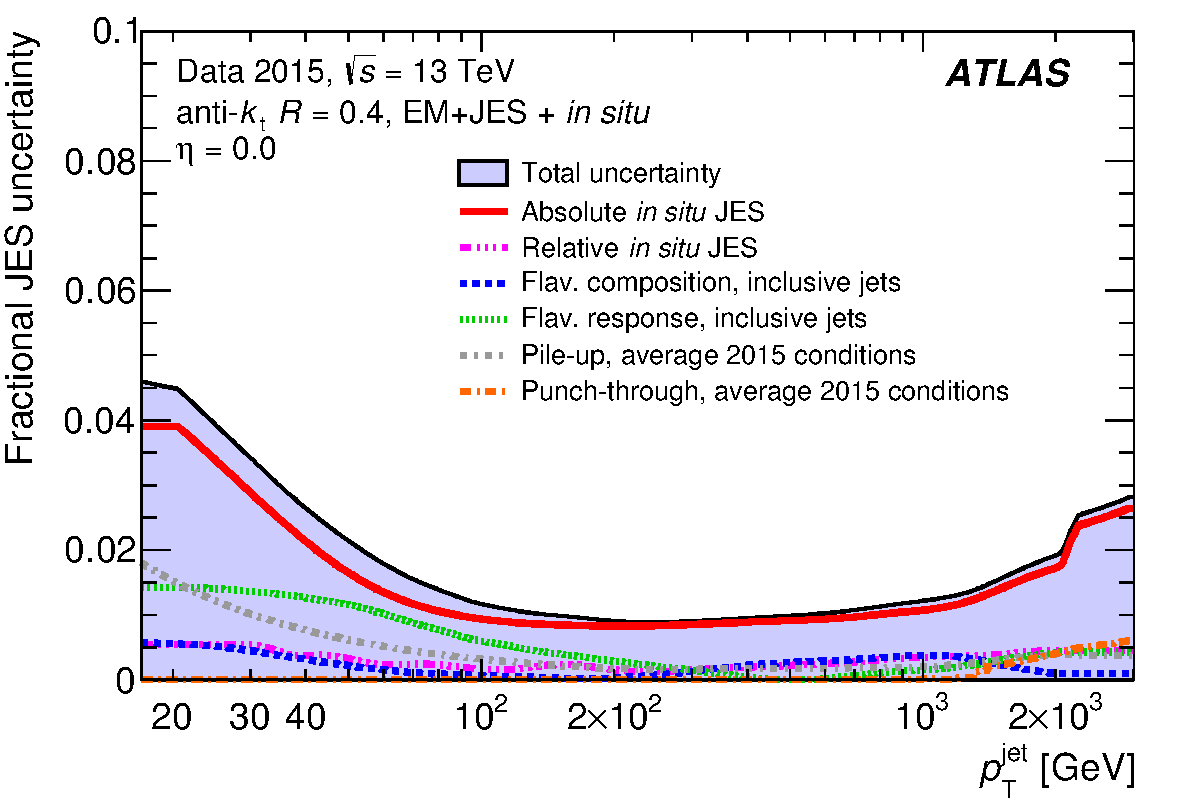
\includegraphics[width=0.48\textwidth]{figures/objects/fig12a.pdf}
  }
  \subfigure[]{
    \label{fig:Comb_syst:eta}
    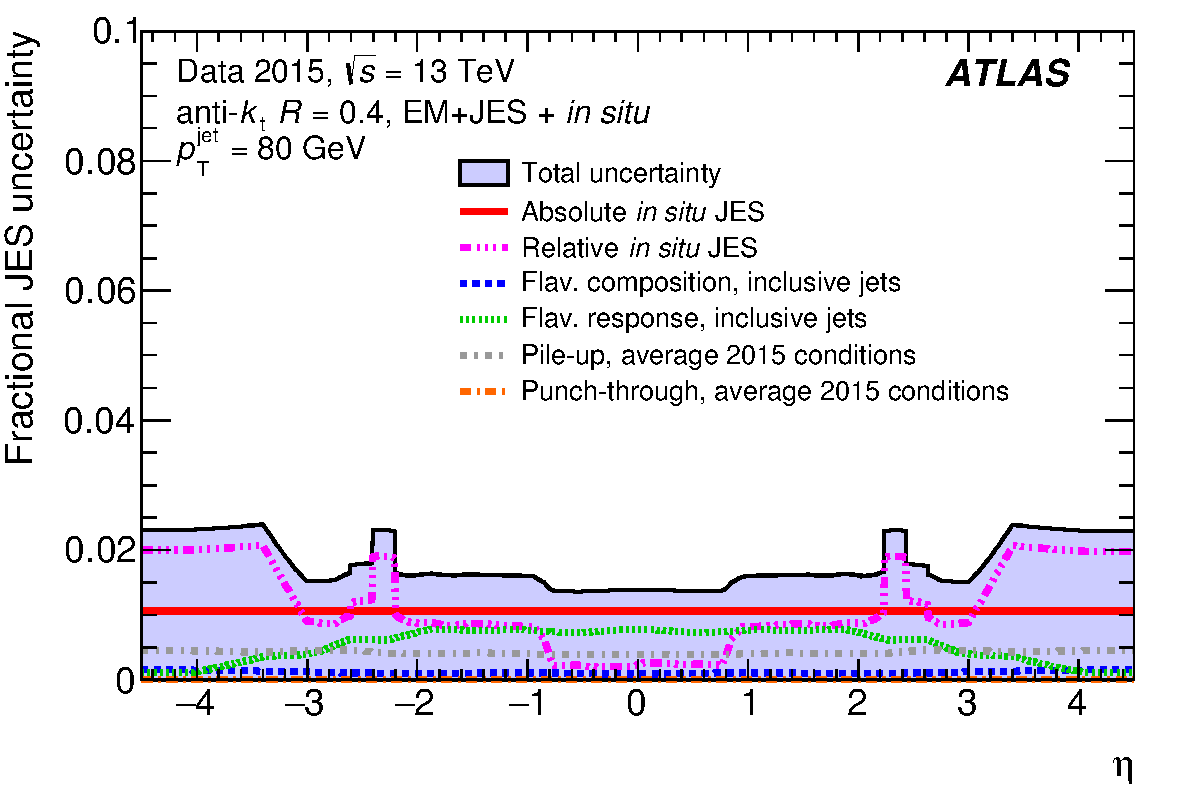
\includegraphics[width=0.48\textwidth]{figures/objects/fig12b.pdf}
  }
\end{center}
 \caption{Combined uncertainty in the \gls{jes} of fully calibrated jets as a function of \subref{fig:Comb_syst:pt}  
 jet \pt at $\eta = 0$ and \subref{fig:Comb_syst:eta} $\eta$ at \pt$ = 80$ GeV. Figure from Ref. \cite{PhysRevD.96.072002}.}
  \label{fig:obj:jessyst}
\end{figure}

To allow an easier usage of the uncertainties in physics analyses, a reduced set of 19 \gls{np} is provided: 
the 67 \glspl{np} from the in-situ calibration are reduced to six by keeping the five uncertainties of largest magnitude, 
plus a sixth one which is the sum in quadrature of the remaining ones. 
A further reduction is in place to group the remaining \glspl{np} into three components, 
and the \glspl{np} within a single component are added in quadrature; this leads to a correlation loss, whose effect is analysis dependent. 

Jets with the same true energy can have different reconstructed energies; the distribution of the difference between true and reconstructed energy of a jet is modeled with a Gaussian, whose width is defined as \gls{jer}. The measurements for the in-situ calibrations can be used also to access the differences in \gls{jer} between data and \gls{mc} \cite{TheATLAScollaboration:2015ofv,ATLAS:2015uwa}, and result into an additional \gls{np}.

\subsection{Jet Vertex Tagger}

It has already been discussed in Sec. \ref{sec:obj:jetcalib} how pileup is taken into account in the calibration of the \gls{jes}. Beside affecting the jet energy, high levels of pileup can also lead to the reconstruction of spurious jets not originating from the hard-scattering interaction. In \gls{atlas} track-based algorithms are used for the identification of pileup jets \cite{Aad:2015ina,ATLAS:2014cva}. 
Tracks are matched to calorimeter jets by ghost-association \cite{Soyez:2012hv}. Once the \gls{pv} is identified, 
for each jet it is possible to compute the \gls{jvf}, the ratio of the scalar sum of the \pt of the tracks associated to the jet and originating from the hard scattering vertex \gls{pv}$_0$ to that of all the associated tracks:

\begin{equation}
 \JVF = \frac{\sum_m{p_{{\rm T}, m}^{{\rm track}}({\rm PV}_0)}}{\sum_n\sum_l  p_{{\rm T}, l}^{{\rm track}}({\rm PV}_n)} \; .
 \label{eq:jvf}
\end{equation} 

\noindent where the index $n$ runs over all the vertices of the event. In high-pileup conditions the denominator in 
Eq. \ref{eq:jvf} increases; to correct for this dependence, the \gls{cjvf} is introduced. 
This is a modified version of \gls{jvf}, that takes into account the dependence on the number of pileup tracks (\nPUtrk):

\begin{equation}
\cJVF = \frac{\sum_m{p_{{\rm T}, m}^{{\rm track}}({\rm PV}_0)}}{\sum_l p_{{\rm T}, l}^{{\rm track}}({\rm PV}_0) + \frac{\sum_{n\geq1}\sum_l p_{{\rm T}, l}^{{\rm track}}({\rm PV}_n)}{ (k \cdot \nPUtrk)}} \; ,
\label{eq:corrJVF}
\end{equation}

\noindent with $k=0.001$. Another variable used to discriminate hard-scattering jets against pileup jets is the ratio of the scalar
sum of the \pt of the tracks originating from \gls{pv}$_0$ to the jet transverse momentum:


\begin{equation}
\RpT = \frac{\sum_k{p_{\rm{T}, k}^{{\rm track}}({\rm PV}_0)}}{\ptjet}
\label{eq:obj:rpt}
\end{equation}

The \cJVF and \RpT are combined in a two-dimensional likelihood that constitutes a single tagger, the \gls{jvt}. 
The distribution of \gls{jvt} for hard-scattering and pileup jets in \gls{mc} simulation is shown in Fig. \ref{fig:obj:jvt_mc},
while Fig. \ref{fig:obj:jvt_data} shows the comparison of the \gls{jvt} distribution in data and \gls{mc} in a di-muon selection.


\begin{figure}[h]
\begin{center}
  \subfigure[]{
    \label{fig:obj:jvt_mc}
    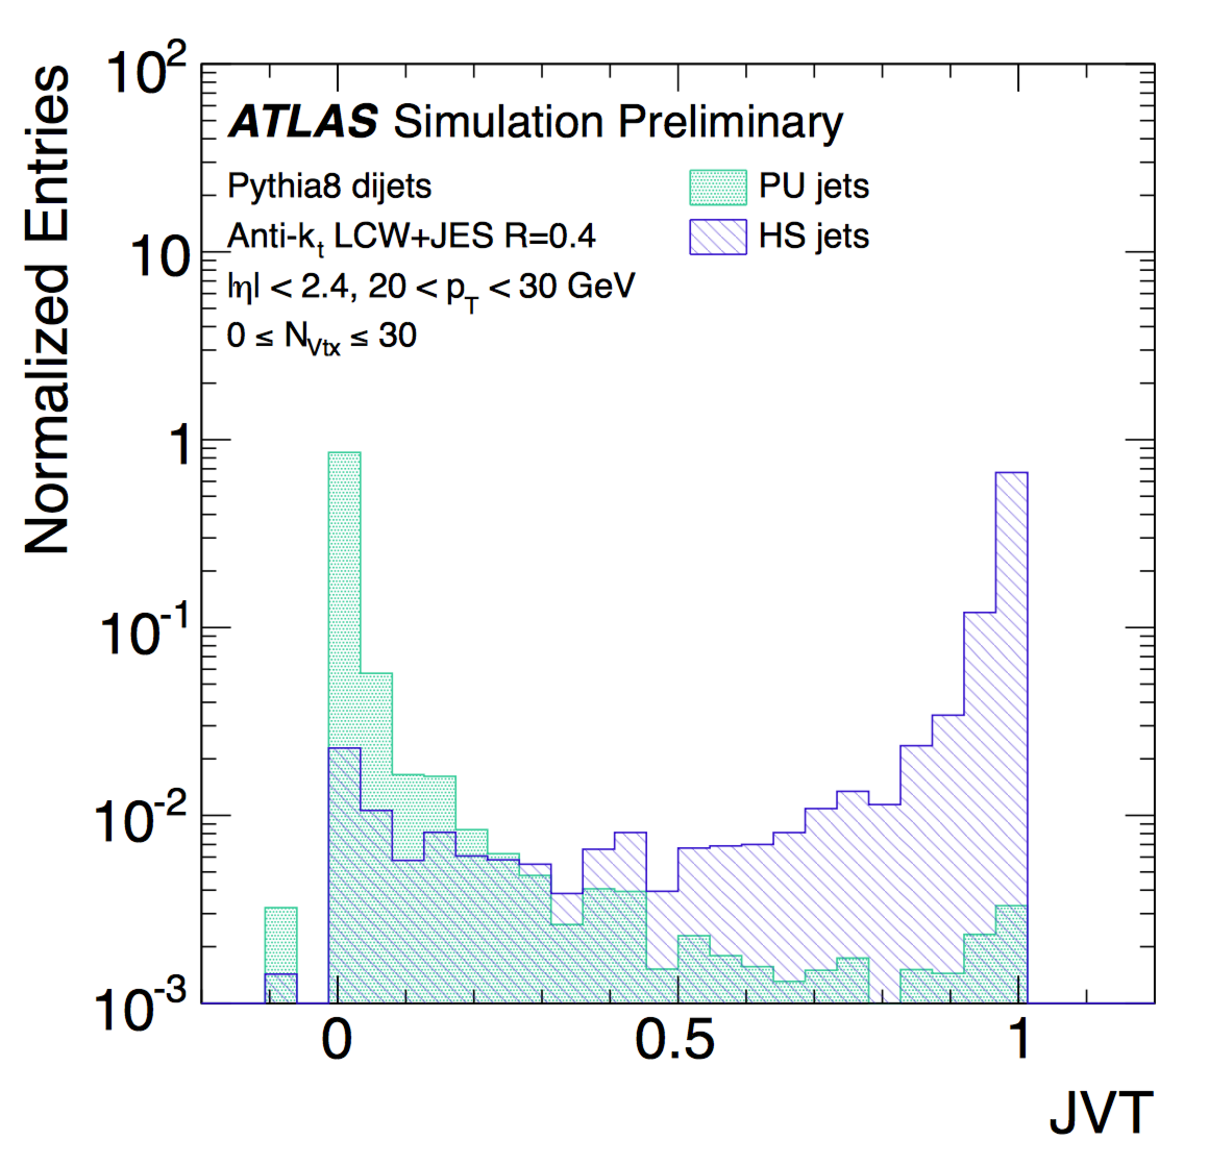
\includegraphics[width=0.43\textwidth]{figures/objects/jvt.pdf}
  }
  \subfigure[]{
    \label{fig:obj:jvt_data}
    \includegraphics[width=0.53\textwidth]{figures/objects/jvt_data.png}
  }
\end{center}
 \caption{\subref{fig:obj:jvt_mc} Distribution of JVT for pileup and hard-scatter jets with $20 < \pt < 30$ GeV. Figure from Ref. \cite{ATLAS:2014cva}. \subref{fig:obj:jvt_data} The JVT distribution, in Powheg+Pythia8 MC and in 2015+2016 data, of jets balanced against Z bosons decaying to muons. Figure from Ref. \cite{jvtpublicplots}.}
  \label{fig:obj:jvt}
\end{figure}

\subsection{Jet Cleaning}

Beside pileup jest, other spurious jets come from the \gls{ncb}; this type of background includes muons originating from secondary cascades from beam losses (in this case we speak of \gls{bib}) and from cosmic rays. These muons that leave energy deposits in the calorimeters while traversing the detector, that can be interpreted as jets. Also coherent noise from the calorimeters can give rise to fake jets. In \gls{atlas} a set of quality criteria are designed to reject jets not originating from \gls{pp} collisions \cite{TheATLAScollaboration:2015ofz}. These quality criteria are rely on variables built based on:
\begin{itemize}
\item Ionization signal shape in the LAr calorimeters, to remove mainly fake jets from calorimeter noise. 
\item Ratios of energies, for example the ratio of the energy deposited in the electromagnetc calorimeter to the total energy, or the ratio of energy in different calorimeter layers, that can be used to discriminate against jets from \gls{bib} or calorimeter noise.
\item Tracks associated with the jets, and in particular variables similar to \RpT defined in Eq. \ref{eq:obj:rpt}, that have in general lower value for fake jets than for jets originating from \gls{pp} collisions. 
\end{itemize} 

Different thresholds for the selections on these variable distinguish the two working points, \textit{BadLoose} and \textit{BadTight}, which have an efficiency respectively of 99.5\% and 95\% for jets with $\pt > 20$ GeV (while for jets with $\pt > 100$ GeV the efficiency of the two working points increases to 99.9\% and 99.5\%). 

\subsection{Re-clustered Jets}

The angular separation between the decay products of a particle with mass $m^P$ and transverse momentum 
$p_T^P$ scales as:
\begin{equation}
\Delta R \approx \frac{2 m^P}{p_T^P} \; .
\end{equation}

This indicates that the ideal value of the $R$ parameter described in Sec. \ref{sec:obj:jetfinding} can vary depending on the event topology that we want to capture;
for example, the decay products of an heavy particle with a transverse momentum much larger than its rest mass (\textit{boosted object}) could be better described by a 
single jet with a larger $R$ than with multiple jets with the "standard" 0.4 radius, 
as it happens for example in the decay of very energetic top quarks, W, Z or Higgs bosons produced at the LHC.
Each different value of the $R$ parameter requires a dedicated calibration following the steps described in Sec. \ref{sec:obj:jetcalib}. 
Therefore, it is not always possible to choose the optimal value of the jet radius. 
A possible solution to this problem comes from noticing that the same jet-finding algorithms used to group topoclusters can have different types of inputs. 
In particular, jets themselves can be be used as input and grouped together, and in this case we speak of \textit{re-clustered jets} \cite{Nachman:2014kla}. 
The re-clustered jest are automatically calibrated as long as the input jets are, and also the jet uncertainties can be propagated directly. 
A comparison of the jet clustering obtained with $R$=1.0 anti-$k_T$ and by re-clustering anti-$k_T$ $R$=0.3 jets into anti-$k_T$ $R$=1.0
is shown in Fig. \ref{fig:recluster}. It is possible to see how the jet axis is similar between the two cases, and how the $R$=1.0 anti-$k_T$ have more inputs away from the jet axis.
Re-clustered jets can be \textit{trimmed} by removing the constituent small-R jets that have a \pt smaller than a defined fraction of the \pt of the original reclustered jet. 


\begin{figure}[h]
\begin{center}
\includegraphics[width=1.0\textwidth]{./figures/objects/reclustered.pdf}
\end{center}
\caption{Example event where jets have been clustered with (a) anti-$k_T$ with $R$=1.0 and (b) anti-$k_T$ $R$=1.0 re-clustered jets (starting from anti-$k_T$ $R$=0.3 jets); the shaded region shows the jet area. Figure from Ref. \cite{Nachman:2014kla}.}
\label{fig:recluster}
\end{figure}

\section{Jets from B-hadrons}

Jets originating from the hadronization of a b-quark (\textit{b-jets}) can be identified thanks to the lifetime of B-hadrons (about $10^{-12}$ s), which is shorter than the typical lifetime of hadrons containing only light quarks, but still long enough to allow the B-hadrons to travel distances of the order of the mm before decaying. A schematic view of the topology originating from a jet containing a B-hadron is shown in Fig. \ref{fig:btag}.


\begin{figure}[h]
\begin{center}
\includegraphics[width=0.45\textwidth]{./figures/objects/secvtx.pdf}
\end{center}
\caption[Schematic view of the topology of a b-jet.]{Schematic view of the topology of a b-jet. Figure from Ref. \cite{d0btagging}.}
\label{fig:btag}
\end{figure}

The procedure of identifying b-jets is referred to as \textit{b-tagging}, and in \gls{atlas} is performed using as input the tracks associated to the jets . As already mentioned in Sec. \ref{sec:atlas:pixel}, between Run 1 and Run 2 a fourth pixel layer (\gls{ibl}) was added to the \gls{atlas} detector, allowing a better impact parameter resolution and therefore improving substantially the b-tagging performance. There are three basic families of algorithms, that can then be combined through multivariate techniques. The basic algorithms can be based on:

\begin{description}

\item[Impact Parameter] The transverse impact parameter of a track (\dzero) is the point of closest approach to the 
\gls{pv} in the transverse plane, while the longitudinal impact parameter (\zzerost) is defined as the distance along 
the $z$-axis between the \gls{pv} and the point of closest approach in the transverse plane. Because of the typical 
lifetime of B-hadrons, on average b-jets contain tracks with higher impact parameter than light-jets. 
A sign can be 
assigned to the impact parameter, that will be positive if the secondary vertex from which the track is originating is 
in front of the \gls{pv}, negative otherwise. The negative side of the impact-parameter distribution derives from the 
impact-parameter resolution, and can be used to calibrate light-jets. Two taggers make use of the information on the impact parameter
 \cite{ATLAS:2011qia}: IP2D, which is based on the significance of the transverse impact parameter (\dzero/$\sigma_\dzero$), and IP3D, which builds a two-dimensional template including also the significance of the longitudinal impact parameter (\zzerost/$\sigma_\zzerost$). The \pdf for each flavour hypothesis (b, c, light) is derived from \gls{mc} simulation on a per-track basis, and then a \gls{llr} of the different probabilities is computed, including the contribution from all the tracks associated to the jet. For example, the \gls{llr} discriminating b-jets from light-jets is of the form $\sum_{i=1}^{N}\log\frac{p_b}{p_{light}}$, where the index $N$ runs on the tracks associated to the jet. 

\item[Secondary Vertex Finding] The secondary vertex finding algorithm \cite{ATLAS:2011qia} explicitly looks for a secondary vertex within a jet. 
All the track pairs in the jet are tested for a two-track vertex hypothesis, removing the pairs that are likely to originate from 
long-lived particles (e.g. K$_0$, $\Lambda$), photon conversion or hadronic interaction with the detector material. 
If a two-track vertex remains, a new single vertex is fitted with the tracks passing this selection.

\item[Identification of the Decay Chain] The b-hadrons inside b-jets decay with an electroweak interaction, 
through which a b-quarks decays preferentially into a c-quark (since the CKM matrix element $|V_{cb}|^2$ is much larger than $|V_{ub}|^2$). Hadrons containing a c-quark (D-hadrons) subsequently decay as well, giving rise to a topology with two decay vertices. While the resolution is often not enough to reconstruct the two vertices individually, the JetFitter algorithm \cite{1742-6596-119-3-032032} operates assuming that they both lie on the same line, the flight axis of the B-hadron. The information on the event topology derived with JetFitter is then used in likelihood function, from which three different templates (one for each flavour) are derived.

\end{description}

The default b-tagging algorithm used by \gls{atlas} in the analysis of the 2015-2016 dataset is MV2c10 
\cite{ATL-PHYS-PUB-2015-022,ATL-PHYS-PUB-2016-012}, 
a multivariate algorithm based on a \gls{bdt} that combines the output of the algorithms described above. 
MV2c10 belongs to the family of MV2 algorithms, that are trained on a \ttbar sample, using b-jets as signal and c-jets and light-jets as background, differ in the relative fraction of c-jets and light-jets that are
used in the training; in the case of MV2c10, the background sample in the training contains 15\% of c-jets.
Fig. \ref{fig:obj:mv2} shows the light-jet and c-jet rejection as a function of b-jet efficiency for different MV2 algorithms.

\begin{figure}[h]
\begin{center}
  \subfigure[]{
    \label{fig:obj:mv2_a}
    \includegraphics[width=0.48\textwidth]{figures/objects/mv2c10_a.pdf}  }
  \subfigure[]{
    \label{fig:obj:mv2_b}
    \includegraphics[width=0.48\textwidth]{figures/objects/mv2c10_b.pdf} }
\end{center}
 \caption{Light-jet \subref{fig:obj:mv2_a} and c-jet \subref{fig:obj:mv2_b} rejection as a function of the b-jet efficiency for the MV2 algorithms. Figures from Ref. \cite{ATL-PHYS-PUB-2016-012}.}
  \label{fig:obj:mv2}
\end{figure}

\glspl{op} are defined by a selection on the value of the \gls{bdt} output, and are designed to have a specific b-jet efficiency.
Table \ref{tab:obj:mv2op} shows the \glspl{op} of the MV2c10 algorithm.

\begin{table}[h]
\begin{center}
    \includegraphics[width=1.0\textwidth]{figures/objects/btag_op.pdf}  
\end{center}
 \caption{Operating points for the MV2c10 b-tagging algorithm. The efficiency and rejection rates are computed for jets with $\pt > 20$ GeV from \ttbar events. Table from Ref. \cite{ATL-PHYS-PUB-2016-012}.}
  \label{tab:obj:mv2op}
\end{table}

\subsection{B-tagging Calibration and Uncertainties}

The b-tagging efficiency can be different in \gls{mc} simulation and data. The b-tagging efficiency, 
c-tagging efficiency and light mistag rate are measured in data for the \glspl{op} of Table \ref{tab:obj:mv2op}, 
and the \gls{mc} simulation is corrected with the \glspl{sf} derived as the ratio of the efficiency in data and in \gls{mc}. 
The \glspl{sf} are derived on a per-jet basis in a parametric form based on jet \pt, $\eta$ and truth flavour. 
For each \gls{mc} simulated event, an event-level \gls{sf} is derived by multiplying all the efficiency \glspl{sf} for the b-tagged jets 
and all the inefficiency \glspl{sf} for the jets that are not b-tagged. Different techniques are used in \gls{atlas} to measure the b-tagging 
efficiency in \gls{atlas} for the different jet flavours \cite{1748-0221-11-04-P04008}.
The calibrations used in the analyses described in this thesis are:

\begin{description}

\item[b-jets] The default b-tagging calibration for b-jest is based on a \ttbar dileptonic sample. Events with exactly two opposite-sign leptons
and two or three jets are selected, and a per-event likelihood is built containing the b-tagging weight \gls{pdf} for a jet of a given flavour;
the \gls{pdf} for light-jets and c-jets is taken from \gls{mc}, while the \gls{pdf} for b-jets is the information that we want to extract from data.
This last \gls{pdf} is described by a histogram with only two bins, one below and one above the threshold to b-tag a jet. 

%\gls{bdt} based on 8 input variables 
%Likelihood fit using per-jet flavour correlations. 

\item[c-jets] The analysis described in Chapter \ref{chap:strong_prod} uses a c-jet calibration based on events where a W boson 
is produced in association with a c-quark. The events selected are the ones where the W boson decays into an electron and a neutrino,
and the D-hadron originating from the fragmentation of the c-quark decays leptonically (and in particular to a muon). 
In W+c production the electron and the muon in the final state have opposite charge, 
while most of the background processes have an equal number of same-sign and opposite-sign events. The number of W+c events can therefore 
be obtained as the difference of these two categories.
For the analysis described in Chapter \ref{chap:ewk_prod}, that was developed at a later time, a new calibration for c-jets, 
based on \ttbar events \cite{ATLAS:2018bpl}, was available. 
This calibration selects \ttbar events where one of the $W$ bosons decays leptonically and the other one decays to a c-quark and an s-quark. 

\item[light-jets] The b-tagging efficiency of light-jets (mistag rate) is calibrated on an inclusive sample of jets, using the negative tag method.
The two main reasons that lead to b-tagged light-jets are the finite resolution of the impact parameter and the secondary vertices caused
by long-lived particles and material interaction. If we consider only the first type of mistags, the signed impact parameter distribution 
will be symmetric around zero. 
The negative tag method is based on a modified version of the b-tagging algorithms, that takes as input impact parameters and decay lengths with
reversed sign. The mistag rate is measured as the negative-tag efficiency of the jet sample, with \gls{mc}-based correction factors that take into account 
the negative-tag rate for b- and c-jets and the effect of long-lived particles and material interactions.

\end{description}

The b-tagging scale factors are affected by multiple sources of uncertainty, that are reflected in uncertainties on the \glspl{sf}.
As an example, Figure \ref{fig:obj:btagSF} shows the b-tagging \gls{sf} for c-jets derived with the \ttbar calibration for the
77\% \gls{op}. \note{Plots for other calibrations will be added if related CONF is released}.

\begin{figure}[h]
\begin{center}
  \subfigure[]{
    \label{fig:obj:ttSF}
    \includegraphics[width=0.48\textwidth]{figures/objects/cjettt_77SF.png}  }
  %\subfigure[]{
   % \label{fig:obj:mv2_b}
    %\includegraphics[width=0.48\textwidth]{figures/objects/mv2c10_b.pdf} }
\end{center}
 \caption{B-tagging \gls{sf} for c-jets for the \gls{op} corresponding to a 77\% efficiency on \gls{mc} \ttbar. Figure from Ref. \cite{ATLAS:2018bpl}.}
  \label{fig:obj:btagSF}
\end{figure}


\section{Muons}

Muon reconstruction and identification \cite{Aad:2016jkr} is based on the information collected by the \gls{id}, where muons are reconstructed as charged tracks, and by the \gls{ms}. 

\subsection{Muon Reconstruction}

Both devices perform the reconstruction
of muon candidates independently and then the information is combined to build the muon candidates used in physics analyses. 
The reconstruction of muon tracks in the \gls{id} proceeds as described in Section \ref{sec:reco:tracks}. In the \gls{ms}, the first step is the identification of segments starting from the hits in each chamber. A muon track is reconstructed with a segment-seeded search (considering first the segments in the central layers of the detector as seeds, and then extending to the inner and outer ones). Except from the transition region between the barrel and the end-cap, tracks are required to have at least two matching segments; the hits associated to each track are fitted with a global \chis, and the track candidate is accepted or rejected based on the \chis value. 

Reconstructed muons can belong to four different types, depending on the subdetectors that contribute to the reconstruction:

\begin{description}
\item [Combined] Combined muons are built from a global fit that uses hits from tracks reconstructed independently in the \gls{id} and \gls{ms}.
\item[Segment-tagged] Muons of lower \pt or that cross regions of lower acceptance of the \gls{ms} can result in a segment in only one \gls{ms} chamber. If a track from the \gls{id} is associated with this segment, this track is classified as a segment-tagged muon.
\item[Calorimeter-tagged] A track in the \gls{id} is identified as a calorimeter-tagged muon if it is matched to an energy deposit in the calorimeter compatible with a minimum-ionizing particle. This muon category recovers identification efficiency for the muons that fall out of the \gls{ms} acceptance.
\item[Extrapolated] Extrapolated muons are reconstructed from tracks in the \gls{ms} compatible with originating from the \gls{ip}, to recover muons in high-$\eta$ regions, outside of the \gls{id} acceptance.
\end{description}

When multiple types of muon are reconstructed for the same physical object, the redundant ones are removed with an \gls{or} procedure that, when muons share the same \gls{id} tracks, gives priority to combined muons, and then to segment-tagged muons over combined muons. The \gls{or} with extrapolated muons gives preference to the \gls{ms} track with the best quality.

\subsection{Muon Identification}

The reconstructed muons have to fulfill identification criteria that help rejecting the background constituted mostly by decays of pions and kaons. 
The variables used in the identification are the significance of the difference of the charge-over-momentum ration measured by the \gls{id} and by the \gls{ms} ($\frac{q}{p}$ significance),
the difference of the \pt measured in the \gls{id} ad in the \gls{ms} divided by the \pt of the combined track ($\rho'$),
the normalized \chis of the combined fit,
and the number of hits in the different detector layers. 
Based on these quantities, four muon identification criteria are defined: Loose, Medium, Tight and High-\pt. 
Loose, Medium and Tight are inclusive categories with increasingly tighter requirements, while the High-\pt selection starts from the Medium selection and applies extra requirements that improve the momentum resolution for muons with \pt above 100 GeV.

The Medium identification criteria is the default in \gls{atlas}, and is the one that minimizes the systematic uncertainties associated with 
the muon reconstruction and calibration. In the pseudorapidity region with $|\eta|<2.5$, Medium muons are required to be combined muons with $\geq$ 3 hits in at least two \gls{mdt} layers (unless $|\eta|<0.1$, in which case the requirement becomes on one \gls{mdt} layer, but with a hole veto), while extrapolated muons are used when $2.5<|\eta|<2.7$. To suppress muons from hadron decays, the $\frac{q}{p}$ significance is required to be less than seven. 

\subsection{Muon Efficiency Measurement}

In the regions with $|\eta|<2.5$, where the information from both the \gls{id} and the \gls{ms} is available, 
the reconstruction efficiency is measured with a tag-and-probe method, performed on $J/\Psi \rightarrow \mu \mu$ and $Z\rightarrow \mu \mu$ events for low-\pt and high-\pt muons respectively. 
After a selection on the event topology to reduce the background fraction, one of the two muons of the decay is required to be identified 
as a Medium muon. The second leg of the decay (the one to probe) has to be reconstructed by a system independent on the one to be calibrated. For example, calorimeter muons can be used to measure the efficiency of muon identification in the \gls{ms}, while the \gls{id} efficiency can be measured with respect to muons identified in the \gls{ms}. 
The reconstruction efficiency of the Medium \gls{op} as derived from $Z\rightarrow \mu \mu$ and $J/\Psi \rightarrow \mu \mu$ events is shown in Fig \ref{fig:obj:muon_reco}.
The efficiency for high-$\eta$ muons, for which the \gls{id} information is not available, is measured following the same strategy detailed in Ref. \cite{Aad:2014rra}.

\begin{figure}[h]
\begin{center}
  \subfigure[]{
    \label{fig:obj:muon_reco}
    \includegraphics[width=0.48\textwidth]{figures/objects/muon_reco.eps} }
  \subfigure[]{
    \label{fig:obj:muon_iso}
    \includegraphics[width=0.48\textwidth]{figures/objects/muon_iso.eps}  }
\end{center}
 \caption{ \subref{fig:obj:muon_reco} Reconstruction efficiency for the Medium muon selection as a function of the muon \pt, in the region with $0.1<|\eta|<2.5$, as derived from $Z\rightarrow \mu \mu$ and $J/\Psi \rightarrow \mu \mu$ events. 
 \subref{fig:obj:muon_iso} Efficiency of the muon isolation criteria for the \gls{op} $LooseTrackOnly$ as derived from $Z\rightarrow \mu \mu$  events.
 In both figures, the top panel shows the efficiency for data and \gls{mc}, while the bottom panes shows the ratio of data to \gls{mc} with the corresponding uncertainty.
 Figures from Ref. \cite{Aad:2016jkr}.}
  \label{fig:obj:muon}
\end{figure}

\subsection{Muon Isolation}
\label{sec:muoniso}

While muons originating from semileptonic decays of hadrons are very close to the axis of a jet, prompt muons are typically well separated from other physics objects in the event (isolated). The isolation requirements help therefore suppressing further the background from semileptonically decaying hadrons. Different isolation requirements are available and calibrated in \gls{atlas}, defined to be optimal of different analyses. 
The \gls{op} used in the analyses described in this thesis is the one labeled $LooseTrackOnly$, which applies a selection on the ratio of the 
variable \ptvar over the muon \pt (\ptmu), where \ptvar is defined as the scalar sum of the momenta of the tracks with $\pt>1$ GeV in the cone with 
$\Delta\mathrm{R} < \min \left(  10 \, \mathrm{GeV}/\ptmu , \, 0.3\right) $. The \pt-dependent size of the isolation cone helps in recovering efficiency for muons deriving from the decay of boosted particles. The efficiency of the isolation \glspl{op} is calibrated on $Z\rightarrow \mu \mu$ with the tag-and-probe method. The $LooseTrackOnly$ \gls{op} has an efficiency of 99\%, almost constant in $\eta$ and \pt, as shown in Fig. \ref{fig:obj:muon_iso}. 

%\subsection{Momentum Calibration}
%A set of corrections based on the muon \pt and $\eta$ are applied to the \gls{mc} simulation, such that after the correction the simulation describes the muon momentum and momentum resolution in data with a precision of the order of few per-mill and few percent respectively. 
%The corrections are derived in $J/\Psi \rightarrow \mu \mu$ and $Z\rightarrow \mu \mu$ events 

\section{Electrons}

When electrons traverse the \gls{atlas} detector, they leave a track in the \gls{id} and then the energy of their \gls{em} shower is absorbed in the \gls{ecal}.

\subsection{Electron Reconstruction}

The electron reconstruction \cite{ATLAS:2011lah,Aad:2014nim,ATLAS:2016iqc} starts with the identification of clusters in the \gls{ecal}. 
The \gls{ecal} can be divided in a grid of towers of size $0.025\times0.025$ in $\eta$ and $\phi$, and the tower energy is the sum of the 
energy of all the cells belonging to the tower. 
While, in the case of hadronic jets, the calorimeter clusters are created with a topological 
algorithm, in the case of electrons the calorimeter clusters are based on a sliding-window algorithm \cite{Lampl:2008zz} 
with a size of $3\times5$ in units of $0.025\times0.025$ in the ($\eta$, $\phi$) space, that searches for seed towers; these are the centers around which clusters are built.   

The identified clusters are the starting point to reconstruct electrons, photons and converted photons. The key feature that allows to separate electrons from converted and unconverted photons is that, in the case of electrons, the calorimeter clusters are associated with a track from the \gls{id}; instead, in the case of converted photons the cluster is associated with a conversion vertex, while there is no track associated to an unconverted photon. Tracks from the \gls{id} are extrapolated to the second layer of the \gls{ecal}, and a track is considered loosely matched to a seed cluster if the $\eta$ difference between the track and the barycentre of the cluster is lower than 0.05 and the $\phi$ difference either lower than 0.2 (0.1 in the case of tracks deriving from hits only in the \gls{trt}) in the bending direction, or lower that 0.05 in the opposite direction. 
The tracks loosely matched with these criteria are then re-fitted with a Gaussian Sum Filter algorithm \cite{ATLAS:2012dma}, that takes into account non-linear bremsstrahlung effects, and the re-fitted tracks are matched with 
the clusters with the same criteria as the loose matching, except from the $\phi$ difference in the direction of the bending, which is tightened to 0.1. If multiple tracks are associated to a cluster, only one is chosen as primary track based on the cluster-track distance.

After the cluster-track matching, the cluster is re-built using groups of $3\times7$ ($5\times5$) towers in the barrel (endcaps). 

Once the electron is reconstructed, its energy is obtained from the energy of calorimter cluster calibrated to the 
original electron energy with multivariate techniques \cite{Aad:2014nim}, while the $\eta$ and $\phi$ coordinates 
derive from the primary associated track.

Selections on the parameters of the primary track are applied to ensure that the electron is compatible with the \gls{pv} interaction. 
In particular, in Run 2 analyses these selections are: \dzero/$\sigma_\dzero < 0.5$ and  $\zzerost < 0.5$ mm.


\subsection{Electron Identification}

After the electron candidates are reconstructed, a likelihood-based discriminant is used to reject the background, 
constituted mostly by hadronic jets and converted photons. 
This discriminant is built using as signal and background samples $Z\rightarrow e e$ and dijet events fir the
high-\et region, $J/\Psi \rightarrow e e$ and minimum bias events for the low-\et region.
Several variables are used to discriminate between signal and background, based on ratios of energy released in different layers of 
the calorimeter, shape of the \gls{em} shower, quality of the track and of the track-cluster matching; 
the full list of variables is reported in Table \ref{tab:obj:elev_var}.
The variables counting the number of hits in the different layers, as well as $E/p$, $w_\mathrm{stot}$ and 
$\Delta\phi_2$ are used to apply simple selections, while for the other discriminating variables \glspl{pdf} are built based
on the signal and background samples.

\begin{table}[h]
\begin{center}
    \includegraphics[width=0.985\textwidth]{figures/objects/ele_var_tab.pdf}  
\end{center}
 \caption{Definitions of electron discriminating variables. Table from Ref. \cite{ATLAS:2016iqc}.}
  \label{tab:obj:elev_var}
\end{table}

The product of these \glspl{pdf} constitutes the 
signal and background likelihoods ($\mathcal{L}\rm s$ and $\mathcal{L}\rm s$ respectively), and the final discriminant is given by:

\begin{equation}
 d_\mathcal{L} = \frac{\mathcal{L}\rm s}{\mathcal{L}\rm s + \mathcal{L}\rm b}
\end{equation} 

Three identification \glspl{op} are defined, Loose, Medium and Tight, optimized in bins of $|\eta|$ and \et;
these \glspl{op} are inclusive and with an increasing level of signal purity.
The signal and background efficiency in \gls{mc} samples is shown in Fig. \ref{fig:obj:ele_eff}. It is possible to notice how, with increasing
\et, the signal efficiency increases and the background mis-identification decreases.
 
\begin{figure}[h]
\begin{center}
  \subfigure[]{
    \label{fig:obj:ele_eff_e}
    \includegraphics[width=0.48\textwidth]{figures/objects/ele_eff} }
  \subfigure[]{
    \label{fig:obj:ele_eff_bkg}
    \includegraphics[width=0.48\textwidth]{figures/objects/ele_bkg_eff}  }
\end{center}
 \caption{Electron identification efficiency in $Z\rightarrow e e$ events (\subref{fig:obj:ele_eff_e}) and background mis-identification in dijet events (\subref{fig:obj:ele_eff_bkg}) for the three \glspl{op} Loose, Medium and Tight. Figures from Ref. \cite{ATLAS:2016iqc}.
 }
  \label{fig:obj:ele_eff}
\end{figure}


\subsection{Electron Isolation}

As already discussed in the case of muons in Section \ref{sec:muoniso}, prompt signal electrons are in general more isolated than 
electrons candidates originating from hadron decays, from light hadrons misidentified as electrons or from photon conversion. 
The analyses described in this thesis use a track-based isolation criterion, based on the variable \ptvarele, defined as the scalar sum of the \pt 
of the tracks satisfying quality requirements in a cone with $\Delta\mathrm{R} < \min \left(  10 \, \mathrm{GeV}/\et , \, 0.2\right)$, where \et is the transverse energy of the electron candidate and the sum excludes the electron track. The operating point used is $LooseTrackOnly$, 
that applies a selection on the ratio \ptvarele/\et to have an efficiency of 99\% on simulated $Z\rightarrow e e$ events, constant as a function of \et.

\subsection{Electron Efficiency Measurement}

The measurement of the electron efficiency in data relies on the tag-and-probe method, applied to $Z\rightarrow e e$ and $J/\Psi \rightarrow e e$ events, for the high-\et ($> 15$ GeV) and low-\et (typically 7-20 GeV) regions respectively. One of the two electrons is identified with tight criteria and, after kinematic requirements, the second one is used to measure the efficiency.
The electron efficiency is a product of the reconstruction, identification and isolation efficiency 
(and also trigger efficiency, if the events are selected with an electron trigger).  The ratio between the efficiency expected from \gls{mc} simulations and the one measured in data, in the form of \glspl{sf} function of \et and $|\eta|$, is used to correct the simulations and its uncertainty is applied as a systematic variation. 

The identification efficiency is measured with four methods, always with respect to reconstructed electrons. Two methods ($Z_\mathrm{mass}$ and $Z_\mathrm{iso}$) use $Z\rightarrow e e$ events. 
In the $Z_\mathrm{mass}$ analysis, the tag-probe invariant mass is required to be within 15 GeV of the $Z$ boson mass, while in the $Z_\mathrm{iso}$ method the electron isolation is used to discriminate between signal and background. The other two methods \cite{ATLAS:2014wga}, $J/\Psi$ $\tau$-cut and $J/\Psi$ $\tau$-fit, use the distribution of a variable close to the $J/\Psi$ proper time (pseudo-proper time) to select $ee$ events. 
The two $Z$-based methods and the two $J/\Psi$-based methods are combined, taking into account statistical and systematic correlations, to 
derive \glspl{sf} in the high-\et and low-\et regions. 
%As an example, the identification efficiency \glspl{sf} for Tight electrons in the 40-45 \et range, measured in the 2015 data are shown in Fig. \ref{fig:obj:ele_sff_tight}. 
%Fig. \ref{fig:obj:ele_id2016} shows the electron identification efficiency as measured in the 2016 data, for the three \glspl{op} and inclusive in $\eta$. In this second case, the difference between data and \gls{mc} is due to the fact that \gls{mc} simulation do not reflect the changes in the \gls{trt} configuration in 2016 \cite{atlaselec2016}.

%\begin{figure}[h]
%\begin{center}
%  \subfigure[]{
%    \label{fig:obj:ele_sff_tight}
%    \includegraphics[width=0.51\textwidth]{figures/objects/ele_sf_tight} }
%  \subfigure[]{
%    \label{fig:obj:ele_id2016}
%    \includegraphics[width=0.4\textwidth]{figures/objects/ele_ideff_2016}  }
%\end{center}
% \caption{\subref{fig:obj:ele_sff_tight} Identification efficiency \glspl{sf} for Tight electrons in the 40-45 \et range, measured in the 2015 data. Figure from Ref. \cite{ATLAS:2016iqc}. \subref{fig:obj:ele_id2016} Electron identification efficiencies in $Z\rightarrow e e$ events. Figure from Ref. \cite{atlaselec2016}.
% }
%  \label{fig:obj:ele_sf}
%\end{figure}

The reconstruction efficiency is measured as the ratio of reconstructed electrons to the number of \gls{em} clusters. 
It is measured with a method similar to the $Z_\mathrm{mass}$ method, but with the selection criteria for the probe relaxed to include all the \gls{em} clusters. Fig. \ref{fig:obj:ele_eff_pt} shows the combined reconstruction and identification efficiency in $Z\rightarrow e e$ simulated events and in the 2015 data, as a function of \et and inclusive in $\eta$.

\begin{figure}[h]
\begin{center}
  \subfigure[]{
    \label{fig:obj:ele_eff_pt}
    \includegraphics[width=0.48\textwidth]{figures/objects/ele_eff_pt} }
  \subfigure[]{
    \label{fig:obj:ele_}
    %\includegraphics[width=0.48\textwidth]{figures/objects/ele_ideff_2016}  
    }
\end{center}
 \caption{\subref{fig:obj:ele_sff_tight} Combined electron reconstruction and identification efficiency in $Z\rightarrow e e$ simulated events and in the 2015 data, as a function of \et and inclusive in $\eta$. Figure from Ref. \cite{ATLAS:2016iqc}. 
 }
  \label{fig:obj:ele_eff}
\end{figure}

Also the isolation efficiency is measured with a tag-and-probe method derived from the $Z_\mathrm{mass}$ one, but with a lower \et threshold for the 
probe electrons. For each isolation \gls{op}, the efficiency is derived with respect to each identification \gls{op}.

\subsection{Electron Energy Scale and Resolution}

The electron energy scale is measured in $Z\rightarrow e e$ and $J/\Psi \rightarrow e e$ events. 

The electron energy resolution is measured by comparing the width of the $ee$ invariant mass distribution in $Z\rightarrow e e$ events in \gls{mc} simulations and in data.


\section{Missing Transverse Momentum}

Particles that interact only weakly with the detector, such as neutrinos or BSM particles like neutralinos, are not reconstructed directly. 
Their presence is instead inferred by measuring the total momentum imbalance in the event. 

\begin{equation}
\met = \sqrt{(E_{X}^{miss})^{2}  +  (E_{Y}^{miss})^{2}},
\end{equation}

\begin{equation}
E_{X(Y)}^{miss} = E_{X(Y)}^{miss,e} +    E_{X(Y)}^{miss,\gamma} + E_{X(Y)}^{miss,\tau}    \nonumber \\
+ E_{X(Y)}^{miss,jets} + E_{X(Y)}^{miss,soft-terms}  +  E_{X(Y)}^{miss,\mu} 
\label{eq:etm} 
\end{equation}


\begin{equation}
\phi^{miss} = \arctan \left( \frac{E_Y^{miss}}{E_X^{miss}} \right)
\end{equation}

\subsection{\met Trigger}



%\chapter{p-p Interactions and their Simulation}
\label{chap:event:MC}
\glsunset{atlas}

\Gls{pp} interactions at the \gls{lhc} are complex processes that span very different energy scales. 
In order to interpret the experimental data it is essential to develop a good understanding of the physics involved in the \gls{pp} collisions, and the ability to simulate the various processes is also crucial to be able to compare the observed data with the patterns predicted by the theory, first of all the \gls{sm}.
Section \ref{sec:ppint} focuses on the description of our understanding of a \gls{pp} collision, while Section \ref{sec:eventsimul} 
discusses the event-simulation process and the main \gls{mc} generators used in the \gls{atlas} Collaboration. 



\section{p-p Interactions}
\label{sec:ppint}

In hard-scattering processes, where the momentum transfer is much higher than the proton mass \cite{Butterworth:2012fj}, 
a \gls{pp} collision is easier to understand in terms of interactions between the constituents of the protons, quarks and gluons, 
collectively referred to as partons. A schematic view of \gls{pp} event is shown in Fig. \ref{fig:sim:pp2}. In this case, the interaction of a quark and a gluon leads to a final state with a Z boson and jets. 

\begin{figure}[h]
\begin{center}
%  \subfigure[]{
%    \label{fig:Comb_syst:pt}
    \includegraphics[width=0.58\textwidth]{figures/simul/ppcoll2}
%  }
\end{center}
 \caption{Schematic representation of a \gls{pp}, involving a quark-gluon scattering that leads to a final state consisting of a Z boson and a hard jet. Figure from Ref. \cite{Butterworth:2012fj}.}
  \label{fig:sim:pp2}
\end{figure}

As in can be understood from the figure, the hard process, which can be computed in perturbation theory, takes place between two of the proton partons; the probability that a gluon or a specific quark type takes part to the hard scattering is described the \glspl{partdf}, discussed in Section \ref{sec:ppint:hardscatter}. If the products of the hard scattering are quarks or gluons, after loosing energy by radiating other gluons (which in turn can generate quarks through gluon splitting) in the process of parton shower, they evolve into stable hadrons in the lower-energy hadronization process, which we can describe only through phenomenological models.
This picture is further complicated by the fact that also initial-state quarks and gluons can radiate. Also, the other partons not contributing to the hard scattering can interact, originating what is referred to as underlying event. 

\subsection{Factorization Theorem}
\label{sec:ppint:hardscatter}

The hard scattering between the partons inside the proton is in a kinematic regime where the \gls{qcd} coupling constant, $\alpha_s$, 
is small and therefore the partonic cross sections can be computed in perturbation theory. 
Thanks to the factorization theorem \cite{doi:10.1146}, the generic production cross section for a final state $X$ can be expressed in terms of the partonic cross section $\hat\sigma$ as:

\begin{equation}
  \sigma(pp\rightarrow X) = \sum_{i,j} \int dx_1 dx_2\, 
     f_{i}(x_1,\mu_F^2)\, f_{j}(x_2,\mu_F^2)\, 
     \hat\sigma_{ij\rightarrow X}(x_1 x_2 s, \mu_R^2, \mu_F^2) \; .
  \label{eq:general-cross-section}
\end{equation}
The $i$ and $j$ indexes run on all the possible partons, and $f_{i}(x_1,\mu_F^2)$ is the \gls{partdf} for the $i$-th parton, representing 
the distribution of probability for that parton to carry a fraction $x_1$ of the proton momentum when the proton is probed at a scale $\mu_F$
(factorization scale). $\hat\sigma_{ij\rightarrow X}$ is the partonic cross section, computer at the partonic center of mass energy \cmpart;   
it has to be noted that \cmpart is lower than the total center of mass energy, as its square is the product of square of the center of mass energy times
the fraction of the proton momentum that is carried by each of the two partons, $x_1$ and $x_2$. 
While, when considered at all orders in perturbative \gls{qcd}, the partonic cross section does not depend on $\mu_F$,
this dependence appears at any fixed order. $\hat\sigma$ depends also on the renormalization scale, $\mu_R$, which is the scale used for the evaluation of $\alpha_s$.



% factorization theorem 


%\begin{figure}[h]
%\begin{center}
%  \subfigure[]{
%    \label{fig:Comb_syst:pt}
%    \includegraphics[width=0.48\textwidth]{figures/simul/ppcoll2}
%  }
%    \subfigure[]{
%    \label{fig:Comb_syst:pt}
%    \includegraphics[width=0.48\textwidth]{figures/simul/ppcoll}
%  }
%\end{center}
% \caption{Diagrammatic structure of a generic hard-scattering process. Figure from Ref. \cite{Campbell:2006wx}.}
%  \label{fig:sim:pp}
%\end{figure}

\subsection{Parton Density Functions}
\label{sec:protpdf}

The partons inside the proton can not be observed as free particles, and therefore their \glspl{partdf} can not be computed with
perturbative \gls{qcd}. In particular, for a given scale, it is not possible to predict theoretically the probability distribution 
of the momentum fraction. Instead, once the \glspl{partdf} are known for a certain scale, their energy evolution is 
determined by the equations derived independently by Dokshitzer \cite{Dokshitzer:1977sg} , Gribov and Lipatov \cite{Gribov:1972ri}, and Altarelli and Parisi \cite{ALTARELLI1977298} (DGLAP equations):

\begin{equation}
\begin{aligned}
\frac{\partial q(x,Q^2)}{\partial {\rm log}Q^2}~&=~\frac{\alpha_s}{2\pi}~\left( P_{qq} \otimes q~+~P_{qg} \otimes g \right) \, \\
\frac{\partial g(x,Q^2)}{\partial {\rm log}Q^2}~&=~\frac{\alpha_s}{2\pi}~\left( \sum_i P_{gq} \otimes (q_i+\bar{q}_i)~+~P_{gg} \otimes g \right) \; .
\label{eq:glap1}
\end{aligned}
\end{equation}

\noindent In the expressions above, $q(x,Q^2)$ and $g(x,Q^2)$ are the quark and gluon \gls{partdf} respectively, 
$P_{ij}$ describes the $i \to j$ parton splitting function
and $\otimes$ is a symbol for the convolution integral:
\begin{equation}
P \otimes f \equiv \int^1_x\frac{dy}{y}f_q(y)~P\left(\frac{x}{y}\right).
\end{equation}

As mentioned above, the $x$ dependence has to be extracted experimentally. This is done by several collaborations through fits (with typically 10 to 30 parameters) to data of \gls{dis}. As an example, Figure \ref{fig:sim:pp} shows the \gls{nlo} \glspl{partdf} obtained by the MSTW Collaboration for two different scales, Q$^2$ = 10 GeV$^2$ and Q$^2$ = 10$^4$ GeV$^2$. It is possible to notice how, with the increase of Q$^2$, the shape of the \glspl{partdf} changes to favor lower $x$ values. At low $x$ values the gluon \gls{pdf} is dominating (and this effect increases with Q$^2$), while for high $x$ values the \glspl{partdf} of the valence quarks are more relevant.

\begin{figure}[h]
\begin{center}
    \includegraphics[width=0.8\textwidth]{figures/simul/pdf}
\end{center}
\caption{MSTW 2008 \gls{nlo} \glspl{partdf} at Q$^2$ = 10 GeV$^2$ and Q$^2$ = 10$^4$ GeV$^2$. Figure from Ref. \cite{Martin:2009iq}.}
 \label{fig:sim:pp}
\end{figure}


\section{Event Simulation}
\label{sec:eventsimul}

The main steps in the simulation of \gls{pp} collision events consists of:
\begin{itemize}
\item Computation of the matrix element for the hard process.
\item \gls{psh} and matching between \gls{psh} and matrix element.
\item Hadronization and decay of unstable particles.
\item Simulation of the underlying event.
\end{itemize}
In the next sections, each step is summarized in its main features.

\subsection{Matrix Element}

As discussed e.g. in Ref \cite{Skands:2011pf}, the partonic cross section for the production of the final state $X$ starting from the partons $i$ and $j$, necessary to compute
Equation \ref{eq:general-cross-section}, can be expressed at all orders as:
\begin{equation}
\hat\sigma_{ij\rightarrow X} = \sum_{k=0}^\infty \int d\Phi_{X+k} |\sum_{l=0}^\infty \mathcal{M}_{X+k}^{(l)}|^2 \; .
\label{eq:xsec_matrix}
\end{equation}
\noindent In this expression, the $k$ represents the number of final state quarks and gluons produced in addition to $X$ and $\mathcal{M}_{X+k}^{(l)}$
the amplitude to produce the final state $X+k$ computed with $l$ virtual loops. To compute a cross section is not possible to extend these sums to infinity, and the number of extra partons and the number of loops identify the 
perturbative order of the cross section. In particular:
\begin{itemize}
\item The lowest possible order for the production of $X$ is the \gls{lo}, where $k=l=0$.
\item $l=0$, $k=n$ represents the \gls{lo} computation for the production of $X$ + $n$ jets.
\item $k+l \leq n$ corresponds to a N$^n$LO prediction for the production of $X$, while N$^{n-k}$LO for the production of $X$ in association with $k$ jets.
\end{itemize}

At each order, the computation of the matrix element implies a choice of the factorization and renormalization scales.
$\mu_F$ and $\mu_R$ are not predetermined, and are typically set to values related to the scale of the considered physical process. 
The impact of this subjective choice is taken into account by evaluating each production cross section at different scales (typically a variation of a factor two up and down), and assigning the difference as a systematic uncertainty on the cross section estimate.


\subsection{Parton Shower}

The theorem from Kinoshita, Lee and Nauenberg (KLN theorem) \cite{Kinoshita:1962ur,Lee:1964is} guarantees that, 
when computing inclusive cross sections, the logarithmic divergences arising from collinear splitting cancel against the virtual corrections order by order in perturbation theory. 
This does not hold anymore when we are interested in the computation of a differential cross section, for example with a specific number of accompanying final-state extra partons, 
as it could be the case $l=0, k=1$ in Equation \ref{eq:xsec_matrix}. 
In this case, the kinematic of the basic inclusive event is simulated at fixed order, and the \gls{qcd} emission process (splitting) is carried out by the \gls{psh} algorithms \cite{Fox:1979ag}, that generate an ordered sequence of emissions with decreasing angle and energy; the \gls{psh} approximation consists in retaining only the largest matrix elements, namely the ones corresponding to low angles and energies, obtaining a \gls{ll} accuracy.
There are three types of processes that need to be taken care of by the \gls{psh}: $g \rightarrow q\bar{q}$, $g \rightarrow gg$ and $q \rightarrow q g$.
The probability for a parton to evolve from an energy $t$ to a lower energy $t'$ without splitting is encoded in the Sudakov form factor:
\begin{equation}
  \Delta_i(t,t')=\exp\left(-\sum_{j\in\{q,g\}}\,
  \int_t^{t'}\frac{{\rm{d}}\bar{t}}{\bar{t}}\int_{z_{\rm min}}^{z_{\rm max}}{\rm{d}} z\,
  \frac{ \alpha_s }{2 \pi } \, \frac{1}{2} \, P_{ij}(z) \right) \;,
  \label{eq:sudakov_intro}
\end{equation}

\noindent where $P_{ij}$ is the parton splitting function (described in Section \ref{sec:protpdf}).
Equation \ref{eq:sudakov_intro} is sampled with \gls{mc} techniques to produce the sequence of splittings, until the hadronization scale is reached. 

Also incoming particles can emit extra partons, giving rise to \gls{isr}. While in the case of \gls{fsr} the first emissions are harder than the following ones, for \gls{isr} the ordering is inverted, and the showering is performed with a backwards-evolution algorithm \cite{Sjostrand:1985xi}.

\subsection{Matching}

When a process F is simulated with \gls{lo} matrix element plus \gls{psh}, as illustrated in the left diagram in Figure \ref{fig:sim:matching} (following the discussion in Ref. \cite{Skands:2011pf}), the hardest extra jet is at \gls{ll} accuracy. 
One might wish to improve the accuracy of the description of the event by adding the \gls{lo} matrix element for the process F with the addition of one extra parton (F+1), as in the second diagram in Figure \ref{fig:sim:matching}. In this figure, the boxes are only partially filled to indicate the phase-space restriction necessary to deal with the divergence of the F+1 matrix element. Adding naively these two pieces leads to double counting, as illustrated in the third diagram of Figure \ref{fig:sim:matching}. 
This double-counting problem worsens with the increase of the number of extra legs that we want to add at matrix element.

\begin{figure}[h]
\begin{center}
    \includegraphics[width=\textwidth]{figures/simul/matching}
\end{center}
\caption{Illustration of the source of possible double-counting originating from adding matrix elements with different number of legs. Figure from Ref. \cite{Skands:2011pf}.}
 \label{fig:sim:matching}
\end{figure}

Different methods have been designed to match matrix elements to showers such that, for each order in perturbation theory, double-counting is avoided. The three main strategies are \cite{Giele:2011cb}:
\begin{description}
\item[Unitarity] This approach consists in correcting the shower splitting functions by multiplicative factors obtained as the ration of matrix elements to shower approximation:
$$
\rm{Matched} = \rm{Approximate}\frac{\rm{Exact}}{Approximate} \; .
$$
\noindent When these correction factors are inserted in the shower evolution, they guarantee that the shower evolution of the process F describes correctly also the F+1 matrix element, without actually adding the F+1 sample. This strategy, adopted by Powheg and Pythia, had traditionally been worked out only for one extra parton emission. 

\item[Subtraction] The subtraction approach consists in correcting the \gls{psh} by the difference between \gls{psh} and matrix element:
$$
\rm{Matched} = \rm{Approximate} + (\rm{Exact}- \rm{Approximate}) \; .
$$

\noindent With this strategy, the corrections are not resummed and the events are weighted. 

\item[Slicing] The slicing approach divides the phase space into two regions: one described mainly by the matrix elements (by vetoing shower emissions below a cutoff scale, the matching scale), and one mainly by the \gls{psh}:
$$
 {\rm{Matched (above \; matching \;  scale)}} \approx {\rm{Exact}} (1 + {\mathcal{O}} ( \alpha_s)) \; , 
$$
$$
\rm{Matched (below \; matching \;  scale)}  = \rm{Approximate} + (\rm{Exact}- \rm{Approximate}) \approx Approximate    \; ,
$$

\noindent where the last approximation holds because, below the matching scale, the matrix element and the \gls{psh} give similar results. 
Examples of this approach are the CKKW and MLM prescriptions. With the slicing strategy, the corrections are not resummed and the events are weighted, but the weights are all positive. This approach can be extended beyond $\alpha_s$

\end{description}


\subsection{Hadronization and Hadron Decays}

At the end of the shower we have emissions at very low energy and angles, which correspond to high values of the \gls{qcd} coupling constant. 
When the strong coupling becomes of order unit, the interaction is very strong and this is presumably what gives rise to hadronization, the process where colored partons, after parton shower, become a set of colorless hadrons (primary hadrons), 
that can in turn decay into secondary hadrons. This transition is described through phenomenological models since the hadrinization scale, that corresponds also to the \gls{ir} cutoff of the parton shower, is outside the perturbative regime of \gls{qcd}. At the end of the shower, the color, flavour and momentum distribution is already organized, and the hadronization process can only do a local redistribution.
Two main hadronization models are used in \gls{mc} generators:

\begin{description}
\item[String Model] The string model \cite{Artru:1974hr} is based on linear confinement: the potential energy between two colored particles increases linearly with their distance, when the distance is greater than about 1 fm (while at shorter distances also a Coulomb term is present). This terms comprises several different models, among which the most used nowadays is the Lund model \cite{Andersson:1983ia,Andersson:1998tv}. 
A color string forms that joins the the final state in a string configuration of field energies, and hadrons originate from the breakups of the string. The proportionality constant of the linear inter-quark potential can be measured from quarkonia spectra or from lattice \gls{qcd}, and results to be $\approx$ 1 GeV/fm.

The main difference between quarks and gluons resides in the fact that, while quarks are connected to one single string, gluons are connected to two and have therefore a rate for hadron production double than that of quarks. 

% chiara: describe the main steps of the string model hadronization

The fragmentation function determines the probability of a given hadron to carry a certain fraction of the available momentum. In the Lund model the form of the fragmentation function is constrained by the left-right symmetry necessary to make the model independent on the sequence of string breakups. The resulting function depends on the mass and \pt of the hadron, leading to heavier hadrons carrying on average an higher fraction of the momentum.

\item[Cluster Model] The cluster model is based on preconfinement. The clusters of color and anti-color, instead of forming a string, at a sufficient low scale can decay directly into (possibly unstable) hadrons. The mass distribution of the preconfined clusters results to be independent on the scale and nature of the original hard process. This universal distribution of the cluster mass peaks below 1 GeV, with a tail that extends to above 10 GeV; these cluster with very high mass are decayed as a string.  

\end{description}

These two hadronization models have been developed in the 1980's, and since then there has been no fundamental progress in the theoretical understanding of hadronization. 
When the simulation of the events stops before hadronization, it is referred to as "parton-level".

\subsection{Underlying Event}

Protons contain more than one quark, and they can undergo interactions as well, giving origin to multiple parton interactions in the same collision.
These secondary interactions are in general of lower momentum, since the matrix element is larger for low momentum transfer, and will contribute to the activity along the beam direction, less in the transverse plane. 
When the two protons pass through each other the likelihood of having multiple interactions depends on the overlap between the two protons. 
To model the underlying event, the assumption is made that these processes are $2\rightarrow2$ scattering; the matrix element for these diverges at small angle, so the modelling is dependent on the chosen \pt cutoff. 
To model the data, color reconnection between the primary interaction and the underlying event is needed. 

\subsection{Pileup}

\section{MC Generators}

\subsection{General Purpose Generators}

Several independent codes allow to study the effects of different modelling of the hadronization and different choices for the parton shower. The three main general-purpose event generators are:

\begin{description}
\item[Pythia] \cite{Sjostrand:2006za,Sjostrand:2014zea} Uses \pt-ordered parton shower and string hadronization.
\item[Herwig] \cite{Corcella:2000bw,Bahr:2008pv,Bellm:2015jjp} Uses angular-ordered parton shower and cluster hadronization. Gluon splitting processes ($g \rightarrow q\bar{q}$ and $g \rightarrow gg$) in the collinear approximation are not symmetric in the azimuthal direction due to interference of positive and negative helicity states in the original gluon. While Pythia uses a method that takes these affects into account only partially \cite{Webber:1987uy}, Herwig uses one that fully includes spin correlations \cite{Collins:1987cp}. 
\item[Sherpa] \cite{Gleisberg:2008ta} Uses dipole-type parton shower and cluster hadronization. 
\end{description}

The recent versions of all three generators are coded in c++, but Herwig and Pythia were originally developed in Fortran.  

\subsection{Matrix Elements Generators}
\begin{description}
\item[Powheg] 
\end{description}

\subsection{Specialized Generators}


\section{Detector Simulation}

After the detector simulation, the \gls{mc} simulated events are treated in the same manner as data, going through the object reconstruction procedures
describes in Chapter \ref{sec:event:reco}.

\section{Data-driven Corrections}

%\chapter{Common aspects to multi-b+\met SUSY searches}
\label{chap:multib_general}

The main results presented in this thesis are the two analyses described in Chapter \ref{chap:strong_prod} and Chapter \ref{chap:ewk_prod}, which target respectively the strong and electroweak production of supersymmetric particles.
While these analyses target two different benchmark models, they have many commonalities, since both models feature 
a final state rich in $b$-jets and missing transverse momentum (\met). This Chapter highlights these common aspects: 
Section \ref{sec:simplified_models} describes the philosophy of simplified models, used to design and interpret the searches. 
Sections \ref{sec:common_obj_def} and \ref{sec:common_syst} focus on the definition of the physics objects and the experimental systematic uncertainties respectively; Section \ref{sec:common_variables} presents the main kinematic variables used in the analyses 
while Section \ref{sec:common_backgrounds} describes the background sources from \gls{sm} processes, 
how they are modeled in the analyses and the uncertainties on this modelling. 

\section{Simplified models}
\label{sec:simplified_models}

Even with the simplifying assumptions of the \gls{pmssm}, discussed in Section \ref{sec:theory:pmssm}, a \gls{susy} model has to take into account a large number of free parameters, whose values can impact the characteristics of the particle production and decay. 
Simplified models \cite{Alves:2011wf} are very simple models of \gls{bsm} Physics involving only a few particles and decay modes, 
each one focusing on a specific signature, which can be used to optimize and interpret analyses targeting \gls{bsm} scenarios. 
In general simplified models can be viewed as a limit of more complete models, where all particles except a few are too heavy to be 
produced in the interactions. This leads to a drastic reduction of the number of parameters: a simplified model can be described just by the production cross-section and mass of the few particles considered. 
The \glspl{br} of the new particles can be a parameter of the simplified model as well, but it is in general easier to consider each decay chain as a separate simplified model with 100\% \gls{br}.
When simplified models are used to discover or exclude a certain topology, it is important to connect the results obtained to more general models, 
which can be done e.g. by relaxing the restrictions on the \gls{br} of the \gls{bsm} particles or allowing additional particles to take part in the interaction.

\section{Analysis strategy}
\label{sec:analysisstrategy}

The analysis strategy is based on the definition of so-called \glspl{sr}, signal-enriched regions defined by selections on relevant kinematic variables with the goal of maximizing the sensitivity to specific benchmark models. 
After the \glspl{sr} are defined, the key aspect of the analysis is an accurate estimate of the number of events expected from \gls{sm} processes (background events) in these regions, and of the associated uncertainty. 
With the background estimate in hand, it is possible to look at the observed yields in data and compare it with the expectations;
this comparison, performed with the statistical methods discussed in Chapter \ref{chap:stat}, allows quantifying the significance of an excess or placing limits on \gls{bsm} signal models.

The estimate of the expected background events can be performed with different techniques. In particular, in these thesis three types of techniques are used:
\begin{itemize}
\item A first option is to take the background estimate directly from \gls{mc} simulation. 
\item The \gls{mc} estimate can be improved by normalizing each process in a dedicated \gls{cr}, which is a region non overlapping with the \gls{sr}, but kinematically close to it, enriched in the background process that we want to normalize and with a very low expected signal fraction. Since \gls{cr} and \gls{sr} must be non-overlapping, some of the selections of the \gls{sr} are inverted to design the \gls{cr}; the extrapolation of the background normalization factor form the \gls{cr} to the \gls{sr} is tested in dedicated \glspl{vr}. Figure \ref{fig:susy_common:CRschema} shows a schematic view of the relation between \glspl{cr}, \glspl{vr} and \glspl{vr}. A simplified example of how the usage of \glspl{cr} can lead to an improved background prediction with reduced systematic uncertainties is discussed in Section \ref{sec:example_cr}. 
\item In some cases, a background estimate that relies only on data and not on \gls{mc} simulation is preferred. In these cases we speak of a data-driven background estimate.
\end{itemize}

\begin{figure}
\centering
\includegraphics[width=0.55\textwidth]{figures/susy_common/CR_VR}
\caption{Schematic view of the relation between \glspl{cr}, \glspl{vr} and \glspl{vr}. Figure from Ref. \cite{Baak:2014wma}.}
\label{fig:susy_common:CRschema}
\end{figure}
 
In each of the analyses described in this thesis, two different analysis strategies are carried out in parallel:
\begin{description}
\item[Cut-and-count] Several \glspl{sr} are designed, each optimized to maximize the discovery significance to a specific region of the parameter  space, represented by one benchmark model. Cut-and-count \glspl{sr} are useful also to provide simple and powerful model-independent \glspl{ul}, that are easy to re-interpret for signal models different than the ones considered in the analysis. 

\item[Multi-bin] In this case, the \glspl{sr} are non-overlapping. This requirement conflicts with the simple choice of the best selection to maximize the significance, which means that the individual discovery power of each \gls{sr} is smaller than in the case of cut-and-count \glspl{sr}. On the other hand, having non-overlapping \glspl{sr} allows to statistically combine them in the likelihood fit, leading to a stronger model-dependent expected \gls{ul}. The increase in expected exclusion obtained with the combination of several regions is demonstrated in Section \ref{sec:example_combi}.
 
\end{description}


\section{Object definition}
\label{sec:common_obj_def}

Physics objects used in the analyses are defined with two sets of inclusive selections:
a first set of looser selections defines the baseline objects. 
These are used as input for the overlap removal algorithm which, in the steps defined in the next paragraph,
solves the possible double-counting of physics objects (e.g. electrons reconstructed also as jets); objects that survive the overlap removal procedure are then subject to 
tighter selections to define the signal objects. The specific selections applied to jets, electrons and muons are:

\begin{description}

\item[Jets] Baseline jets are reconstructed with the anti-$k_T$ algorithm 
%(described in Section \ref{sec:obj:jetfinding}) 
with radius parameter $R=0.4$ 
and use the calibration procedure discussed in Section \ref{sec:obj:jetcalib}. 
The kinematic selection on baseline candidate jets is  $\pt > 20$ GeV and $|\eta|<2.8$; 
In order to suppress fake jets originating from pileup interactions, jets with $\pt<60$ GeV are required to have \gls{jvt} > 0.59 and satisfy the cleaning criteria discussed in Section \ref{sec:jetcleaning} with the \textit{BadLoose} \gls{op}.
After overlap removal, signal jets are required to have $\pt>30 (20)$ GeV for the analysis discussed in Chapter \ref{chap:strong_prod} (\ref{chap:ewk_prod}); the difference on the \pt threshold 
in the two analyses is related to differences in the signal event kinematics, and will be discussed more in detail in the specific chapters.

Jets are considered $b$-tagged based on the output of the MV2c10 algorithm (see Section \ref{sec:btagging}); in both analyses the \gls{op} used corresponds to an average efficiency of 77\% for $b$-jets from simulated  
\ttbar events, and to a rejection factor of 6, 22 and 134 against jets originating from $c$-quarks, hadronic decays of $\tau$ leptons and light jets respectively. 


\item[Re-clustered jets] Baseline jets that survive the overlap removal are re-clustered with the anti-$k_T$ algorithm into large-R jets of radius $R=0.4$, as described in Section \ref{sec:reclustering}. 
Re-clustered jets are trimmed removing the constituents whose \pt falls below 10\% of the \pt of the re-clustered jet, and are then required to have $\pt>100$ GeV and $|\eta|<2.0$.

\item[Electrons] Baseline electrons have to satisfy the Loose identification \gls{op} (see Section \ref{sec:elec_id}) and required to have $\pt > 20 (5)$ GeV the analysis discussed in Chapter \ref{chap:strong_prod} (\ref{chap:ewk_prod}) and $|\eta|<2.47$. 
After overlap removal, signal electrons are required to satisfy the Tight identification \gls{op} and the $LooseTrackOnly$ isolation \gls{op}, and  to have $\pt > 20$ GeV.
Electrons are matched to the \gls{pv} by requiring $|\dzero/\sigma_\dzero| < 5$ and  $|\zzerost| < 0.5$ mm.


\item[Muons] Baseline muons are required to satisfy the Medium identification \gls{op} (see Section \ref{sec:muon_id}) and to have $\pt > 20 (5)$ GeV in the analysis discussed in Chapter \ref{chap:strong_prod} (\ref{chap:ewk_prod}) and $|\eta|<2.5$. 
After overlap removal, signal muons are required to satisfy the $LooseTrackOnly$ isolation \gls{op} and to have $\pt > 20$ GeV.
Muons are also matched to the \gls{pv} by requiring $|\dzero/\sigma_\dzero| < 3$ and  $|\zzerost| < 0.5$ mm; muons that do not satisfy this selection as considered as cosmic muons, and the events with at least one cosmic muons are vetoed.

\end{description}

The missing transverse momentum is defined considering all the calibrated objects in the event, as described in Section \ref{sec:met}, and uses the \gls{tst} to account for the contribution of
detector signals not associated to reconstructed objects. 

\subsubsection*{Overlap removal}

Potential overlaps between jets, electrons and muons are resolved sequentially with the overlap removal procedure. 
First of all, electrons that are likely to originate form muon bremsstrahlung, i.e. those that lie within $\dR < 0.01$ from a muon candidate, are removed.

Overlaps between jet candidates and electron arise mostly from two reasons. Electrons are reconstructed from deposits in the calorimeter, and are therefore reconstructed as jets as well.
In this case we want to preserve the electron and remove the jet, so we remove any non-$b$-tagged jet that lies within $\dR < 0.2$ from an electron candidate;
an exception is done for $b$-tagged jets, since in this case the electron is likely to originate from a semileptonic $B$-hadron decay. 
Electron candidates that are close to the surviving jets are likely to have been produced in the decay of an hadron inside the jet, and are therefore removed
if they lie within $\dR<0.4$ from a jet and their energy is lower than 50 GeV, or if their energy is higher than 50 GeV and the \dR from the jet 
is lower than min$(0.4, 0.04 + 10 \, {\rm{GeV}}/E_{\rm{T}})$. 
Having an energy-dependent \dR selection aims at increasing the acceptance for leptons originating from the decay of boosted top quarks.

Unlike electrons, muons are unlikely to be reconstructed as jets. Therefore, the first step in the overlap removal procedure between muon candidates and jets 
aims primarily at removing the muons that originate from the decay of hadrons inside the jets. 
Muons and jets can also be close if the jet is originating from muon bremsstrahlung; these jets typically have a small number of associated \gls{id} tracks.
Therefore jets that lie within $\dR < 0.2$ from a muon are removed if they are not $b$-tagged and if they have less than three matching \gls{id} tracks. 
Muons in close proximity to the surviving jets are removed 
if they lie within $\dR<0.4$ from a jet and their \pt is lower than 50 GeV, or if their \pt is higher than 50 GeV and the \dR from the jet 
is lower than min$(0.4, 0.04 + 10 \, {\rm{GeV}}/\pt)$. 

\section{Experimental systematic uncertainties}
\label{sec:common_syst}

Each of the selections in the definition of the objects described in Section \ref{sec:common_obj_def} has an associated experimental systematic uncertainty on the modelling of that selection in 
the \gls{mc} simulation. The experimental systematic uncertainties that are most relevant for analyses targeting final states with multiple $b$-jets and \met are:

\begin{description}

\item[JES and JER] As discussed in Section \ref{sec:obj:jetcalib}, the \gls{jes} and \gls{jer} calibration procedures allow to both calibrate the jet energy from the \gls{em} to the
hadronic scale, and also to correct \gls{mc} simulations to describe better the data; the uncertainties on these corrections propagate to the analyses. 
For the \gls{jes}, reduced sets of uncertainties are available that reduce the number of \glspl{np} to be included in the analysis at the cost of potential loss in correlation; 
the analyses discussed in this thesis use a strongly reduced set with three \glspl{np}. 
Uncertainties on \gls{jes} and \gls{jer} are the leading source of experimental uncertainties, as they can change the kinematic of the jets in the event, and therefore also the number
of jets that fulfill certain selections.

\item[$b$-tagging] The uncertainties on the $b$-tagging calibration procedure (see Section \ref{sec:obj:btaggingcalib}) are included through uncertainties on the $b$-tagging \gls{sf}. 
They are divided into one \gls{np} for the uncertainty on the efficiency of tagging jets originating from $b$-quarks, 
one for the mistagging of the jets originating from 
$c$-quarks, and one for light jets; 
furthermore, one additional \gls{np} for the high-\pt extrapolation uncertainty, based on MC simulation studies, 
increases the uncertainties in the high-\pt region, where the $b$-tagging calibration is not available and the central 
value of the \gls{sf} is taken from the closest calibrated \pt region. 
The uncertainties on $b$-tagging play a relevant role in the analyses in this thesis, as they rely heavily on the selection of events containing $b$-tagged jets.

\item[Luminosity] Besides those uncertainties associated with the object selections, 
another experimental uncertainty that is taken into account in the analysis is 
the uncertainty on the integrated luminosity, whose measurement is described in Section \ref{sec:lumimeas}; for the 2015-2016 dataset the luminosity uncertainty corresponds 
to 3.2\% and is derived with a strategy similar to that described in Ref. \cite{Aaboud:2016hhf}. The impact of this uncertainty on the analyses discussed in this thesis is very small.

\end{description}

\noindent The following systematic uncertainties have been explicitly tested to be negligible in the analyses and are therefore not included in the final results presented in this thesis:

\begin{description}
\item[Leptons] The uncertainties on the calibration and resolution of the energy (momentum) of electrons (muons).
% have been tested to be negligible in all the analyses discussed in this thesis. 

\item[\met] The three \glspl{np} that take into
account the uncertainty on the scale and the parallel and perpendicular resolution of the \met soft term. 
Note that, while the \met soft term uncertainties are not included in the final results, 
the propagation of the \gls{jes} and \gls{jer} uncertainties to the \met computation 
are always properly taken into account.

\end{description}


\section{Common kinematic variables}
\label{sec:common_variables}

The kinematic properties of the objects in the event are used to define variables that, by combining information about multiple objects, 
provide a handle to discriminate between the signal evens from the benchmark model being tested, and the background events from \gls{sm} processes, described in Section \ref{sec:common_backgrounds}. 
While a few of these variables are related to specific characteristics of the signal model, especially in the case of the Higgsino search 
discussed in Chapter \ref{chap:ewk_prod} that involves two Higgs bosons, most of them are built based on the features of the main  
background processes we need to suppress and are therefore in common between the two analyses. 

\subsubsection*{Object energy and multiplicity}

Even just the multiplicity of the objects defined in Section \ref{sec:common_obj_def} provides a powerful handle to analyze the characteristics of an event. In particular, the following multiplicity variables are used:

\begin{description}
\item[\njet] Number of signal jets in the event.
\item[\nbjet] Number of signal jets that are $b$-tagged using the 77\% \gls{op}.
\item[\nlep] Number of signal leptons (electrons and muons) in the event.
\end{description}

\noindent In addition to multiplicity variables, we can also use the energy of the individual objects as a discriminating variable; 
for example, we always consider events with a minimum \met of 200 GeV (the selection is tighter in some \glspl{sr}), 
or we can consider only jets with \pt above a certain threshold if we expect high-\pt jets from the signal. 

\subsubsection*{Effective mass}

The effective mass is defined as the scalar sum of the momenta of all the signal objects in the event and the missing transverse momentum:

\begin{equation}
\meffi = \sum_{i\leq n} {\pt}^{j_i}  + \sum_{j\leq m} {\pt}^{\ell_j}  + \met \; .
\end{equation}

\noindent This variable reflects the overall energy scale of the event, and in the signal is therefore correlated to the mass of the \gls{susy} particles produced. 

\subsubsection*{Transverse mass}

The transverse mass between lepton and \met (\mt) is defined for events with at least one selected signal lepton as: 

\begin{equation}
\mt = \sqrt{2\pt^{\rm{lep}}\met(1-\cos\Delta\phi(\met,\pt^{\rm{lep}}))} \; ,
\end{equation}

\noindent where $\pt^{\rm{lep}}$ is the transverse momentum of the leading signal lepton in the event. 
For events where this lepton and the entire \met derive from the decay of a parent particle with mass m$_{\rm{parent}}$, \mt presents an endpoint at m$_{\rm{parent}}$. 
This is the case when the lepton and \met derive form the leptonic decay of a $W$ boson, in $W$+jets events or in semileptonic \ttbar events; 
note that dileptonic \ttbar events do not present the same endpoint at the W-boson mass, as it is not possible to completely disentangle the energy of the two neutrinos. Events from W+jets or semileptonic \ttbar processes can have values of \mt higher than the kinematic endpoint only if some of the objects in the event are not properly reconstructed (e.g. fake \met from mismeasured jets, jets misidentified as leptons, or leptons out of acceptance).

Another variable useful to suppress the \ttbar background is the minimum transverse mass between \met and the $b$-jets in the event:

\begin{equation}
\label{eq:mtbmin}
\mtb =  \mathrm{min}_{i\leq 3}  \sqrt{(\met+p_T^{j_i})^2 - ({\met}_x+p_x^{j_i})^2 - ({\met}_y+p_y^{j_i})^2 } \; ,
\end{equation}

\noindent where the minimum is taken over the transverse mass computed with the three leading $b$-tagged jets in the event. 
In semileptonic \ttbar events, this variable presents an endpoint near the top-quark mass, as this is the endpoint that we would have if \met originating from the neutrino is perfectly measured and the $b$-jet produced in the decay of the same top quark as the neutrino is among the three leading $b$-tagged jets. 


\subsubsection*{Multijet suppression}

\gls{sm} background events without any neutrino in the decay chain can still have a sizable amount of reconstructed \met if one of the jets in the 
event is mismeasured, leading to a fake energy imbalance in the event. In these cases, the resulting \met will have a value of the azimuthal angle ($\phi$) close to the one of the mismeasured jet. The variable \dphimin is defined as the minimum difference in azimuthal angle between \met and the  four jets with the highest \pt in the event:

\begin{equation}
\dphimin = \textrm{min}_{i \leq 4}(|\phi_{{\rm{jet},}i} - \phi_{\met}|) \; .
\end{equation}

\noindent Requiring high values of this variable helps rejecting events with no real \met. 


\section{Background processes and their modelling}
\label{sec:common_backgrounds}

This section describes the main background processes in the analysis regions, 
which are characterized by the selection of events with an high number of $b$-jets and high \met, and the way they are modeled. 
In general, the modelling is based on \gls{mc} simulations for
all the backgrounds, except multijet which is estimated with a data-driven technique.
For the main background, pair production of top quark pairs (\ttbar), the shape of the different distributions is obtained from \gls{mc}
but the normalization is data-driven, derived in specifically designed \glspl{cr} and tested in \glspl{vr} as described in Section \ref{sec:analysisstrategy}.

\begin{figure}[h]
\centering 
\subfigure[]{\includegraphics[width=0.3\textwidth]{figures/susy_common/feynman/ttbar_4}\label{fig:ttbar_prod_qq}}\\
\subfigure[]{\includegraphics[width=0.3\textwidth]{figures/susy_common/feynman/ttbar_1}\label{fig:ttbar_prod_gg_1}}
\subfigure[]{\includegraphics[width=0.3\textwidth]{figures/susy_common/feynman/ttbar_3}\label{fig:ttbar_prod_gg_2}}
\subfigure[]{\includegraphics[width=0.3\textwidth]{figures/susy_common/feynman/ttbar_2}\label{fig:ttbar_prod_gg_3}}
\caption{\Gls{lo} Feynman diagram for the production of top quark pairs initiated by \subref{fig:ttbar_prod_qq} quark-antiquark annihilation and \subref{fig:ttbar_prod_gg_1}-\subref{fig:ttbar_prod_gg_3} gluon-gluon fusion.}\label{fig:ttbar_prod}
\end{figure}

\subsection{Top quark pair production}
\label{sec:susy_general:ttbar}

Given the presence of several $b$-jets in the final state, \ttbar production in association with jets constitutes the main source of \gls{sm} background in all the analysis regions. \ttbar production, which at the \gls{lhc} at 13 TeV has a cross-section of $831.8^{+19.8 + 35.1}_{-29.2-35.1}$ pb \cite{Czakon:2013goa}, is mediated by the strong interaction, and it can occur through quark-antiquark annihilation (Fig. \ref{fig:ttbar_prod_qq}) or through gluon-gluon fusion (Fig. \ref{fig:ttbar_prod_gg_1} to \ref{fig:ttbar_prod_gg_3}). When the \gls{lhc} is running at 13 TeV, the threshold fraction of the proton energy that must be carried by each parton in order to have sufficient energy to produce a system of two top quarks 
is about 2.6\%.
%, assuming a top quark mass of 173.1 GeV \cite{Patrignani:2016xqp}. 
At these low fractions, the \gls{partdf} of the gluon is higher than the \gls{partdf} of quarks and much higher than the \gls{partdf} of the antiquarks, so gluon-gluon fusion is the dominant \ttbar production mode at the \gls{lhc}.


In the \gls{sm}, the top quark decays $\approx 99.8$\% of the times to a $W$ boson and a $b$-quark. 
Beside the pair of $b$-quarks, which are always present, the final state can be characterized based on the decay of the two $W$ bosons, leading to three different categories:
\begin{description}
\item[Dilepton]  Both $W$ bosons decay to a lepton ($e$, $\mu$, $\tau$) and a neutrino (10.5\%).
\item[Single-lepton] One $W$ boson decays to lepton and neutrino, the other decays hadronically (43.8\%).
\item[All-hadronic] Both $W$ bosons decay hadronically (45.7\%).
\end{description}

All the analysis regions considered in this thesis have a tight \met selection (the loosest one is $\met > 200$ GeV). Since the all-hadronic component 
of the \ttbar background does not have any neutrino in the final state, it does not fulfill the \met requirement unless one or more jets are mismeasured; 
this case produces a negligible background in the analysis regions, and is anyway included in the multijet estimate with the jet-smearing method described in Section \ref{sec:jet_smearing}.
The \ttbar components that is dominating the background estimate are the dilepton and single-lepton ones, both in the analysis regions that require reconstructed leptons as well as in the analysis regions that have a lepton veto.
In the second case, the dominating component is the single-lepton component, where one lepton is a hadronically decaying $\tau$, has a \pt too low to be reconstructed, or falls out of acceptance. 
The \gls{mc} generator used to simulate \ttbar events produced in association with high-\pt jets is \PowhegBox v2 with the CT10 \gls{partdf} set \cite{Lai:2010vv} and interfaced with \PY v6.428 \cite{Sjostrand:2006za} for the \gls{psh} and hadronization. 
The normalization is derived in \glspl{cr} designed to be kinematically as close as possible to the corresponding \glspl{sr} (while being non-overlapping with them by inverting some of the selections), and is expressed in terms of \glspl{sf} relative to the cross-section computed with the highest
available accuracy (NNLO+NNLL \cite{Czakon:2011xx}).

\subsubsection*{Truth-level classification: \ttbar decays}

When considering events at particle level,
the \gls{mc} information can be used to reconstruct the decay chains that lead to the stable particles in the final state. 
Starting from each top quark in the event, it is possible to follow its decay chain and classify the event first of all into dilepton or single-lepton, or also with a finer classification based on the flavor of the lepton. 
Subsequent decays of the $\tau$ lepton are not considered, and hadronically decaying $\tau$ leptons are fully considered as leptons in this classification. 
Figure \ref{fig:ttbar_decay_mT_1L} shows the \ttbar decay type as a function of the \mt value  in a selection requiring at least four jets, at least three $b$-jets, $\met>200$ GeV and at least one signal lepton. It is possible to see that, while at low \mt values the \ttbar component is dominated by events where one top quark decays leptonically and the other one decays hadronically, after the kinematic threshold imposed by the mass of the $W$ boson the dilepton component is dominant. 

\begin{figure}[h!]
\centering 
\includegraphics[width=0.49\textwidth]{figures/susy_common/mc_stack_mT_1L_3b_tt_dec.pdf}
\caption{\ttbar decay type as a function of the \mt value  in a selection requiring at least four jets, at least three $b$-jets, $\met>200$ GeV and at least one signal lepton.}\label{fig:ttbar_decay_mT_1L}

\subfigure[]{\includegraphics[width=0.49\textwidth]{figures/susy_common/mc_stack_mTb_min_1L_3b_tt_dec.pdf}\label{fig:ttbar_dec_mTb_min_1L}}
\subfigure[]{\includegraphics[width=0.49\textwidth]{figures/susy_common/mc_stack_mTb_min_0L_3b_tt_dec.pdf}\label{fig:ttbar_dec_mTb_min_0L}}
\caption{\ttbar decay type as a function of the \mtb value  in a selection requiring at least four jets, at least three $b$-jets, $\met>200$ GeV and \subref{fig:ttbar_dec_mTb_min_1L} at least one signal lepton \subref{fig:ttbar_dec_mTb_min_0L} exactly zero lepton and $\dphimin > 0.4$.}\label{fig:ttbar_decay_mTb_min}
\end{figure}

Figure \ref{fig:ttbar_decay_mTb_min} shows the same \ttbar classification but as a function of \mtb, both in a selection with at least one signal lepton (Figure \ref{fig:ttbar_dec_mTb_min_1L}) and with a lepton veto (Figure \ref{fig:ttbar_dec_mTb_min_0L}). Here it is possible to notice two features. First of all, in general both the selection with a lepton requirement and the one with a lepton veto are dominated by semileptonic decays: in the case of the selection with the lepton requirement the lepton is in most of the cases a muon or an electron, while in the case of the selection with the lepton veto most of the events contain one $\tau$ lepton, which can decay hadronically giving rise to a topology with no electrons or muons.
Secondly, while in the case of \mt \ttbar events are dominating the background composition also for high values of this variable (just with a change from semileptonic to dileptonic \ttbar events), in the case of \mtb after the kinematic endpoint the \ttbar fraction decreases noticeably. 

%\begin{figure}[htb]
%\centering 

%\end{figure}


\subsubsection*{Truth-level classification: flavor of the associated jets}

A truth-level classification is in place to study the \ttbar+jets background based on the flavor of the associated jets.
This is done starting from the \gls{mc} information at particle level; stable particles are grouped into jets using the anti-k$_t$ algorithm 
described in Section \ref{sec:obj:jetfinding} with R=0.4; only particle jets with $\pt > 15$ GeV and $|\eta|<2.5$ are considered. 
The flavor of the jets is determined by matching them with the $B$- and $D$-hadrons that are in a cone of $\Delta R = 0.4$ from the jet. 
If the event contains at least one jet matched to one or more $B$-hadrons, excluding the ones originating from the decay of the top quarks, the event 
is classified as \ttbb. Otherwise, if at least one jet is matched to $D$-hadrons, excluding the ones from the decay chain of the top quarks, the event is classified as \ttcc. \ttbb and \ttcc events are categorized together as \tthf events, where HF stands for heavy flavor, while the remaining ones are classified as \ttlight.
Figure \ref{fig:ttbar_HF_bjets} shows the evolution of the flavor composition of the jets produced in association with \ttbar
as a function of the number of $b$-jets in the event. 
As expected, as the number of $b$-jets increases, the \ttlight fraction decreases and the \ttbb fraction increases. 

\begin{figure}[htb]
\centering 
\subfigure[]{\includegraphics[width=0.49\textwidth]{figures/susy_common/mc_stack_bjets_n_1L_2b_HF.pdf}\label{fig:ttbar_HF_bjets_1L}}
\subfigure[]{\includegraphics[width=0.49\textwidth]{figures/susy_common/mc_stack_bjets_n_0L_2b_HF.pdf}\label{fig:ttbar_HF_bjets_0L}}
\caption{Evolution of the flavor of the jets produced in association with \ttbar in a selection requiring at least four jets, at least two $b$-jets, $\met>200$ GeV and \subref{fig:ttbar_HF_bjets_1L} at least one signal lepton \subref{fig:ttbar_HF_bjets_0L} exactly zero lepton and $\dphimin > 0.4$.}\label{fig:ttbar_HF_bjets}
\end{figure}


\subsubsection*{Modelling uncertainties}

The modelling uncertainties on the \ttbar background considered in this thesis are:
\begin{description}
\item[Generator] The uncertainty associated with the choice of a specific \gls{mc} generator is estimated by comparing \PowhegBox with \aNLO, both interfaced with \HWpp v2.7.1 with the UEEE5 underlying-event tune.

\item[Parton shower and hadronization] Also the choice of the generator that emulates the \gls{psh} and the hadronization is associated to an uncertainty, that is evaluated by comparing the nominal sample, generated with \PowhegBox and showered with \PY, to another sample generated again with \PowhegBox but showered with \HWpp v2.7.1. 

\item[Radiation] The systematic uncertainty related to the modelling of the \gls{isr} and \gls{fsr} is estimated by comparing samples
generated with \PowhegBox interfaced with two versions of \PY v6.428 with two different settings. One uses the PERUGIA2012radHi tune, has $h_{\rm{dump}}$ parameter set to twice the top mass and the renormalization and factorization scales set to twice the nominal value; these settings lead to an overall larger amount of radiation. The second sample uses a version of \PY with the PERUGIA2012radLo tune, has $h_{\rm{dump}}$ set to the top mass and the renormalization and factorization scales set to half of the nominal value, leading to a description of the event with less additional jets.

\end{description}

Figures \ref{fig:ttbar_nj_0L_syst} and \ref{fig:ttbar_ptj1_0L_syst} show the changes in shape in the distribution of the number of signal jets and the \pt of the leading jet when comparing these systematic variations in a representative selection with a lepton veto.
The normalization of \ttbar events is derived in the \glspl{cr}, therefore modelling uncertainties affect only the extrapolation from 
the \gls{cr} to the corresponding \glspl{sr} and \glspl{vr}, and not the overall normalization. 
The modelling uncertainties are therefore estimated by comparing the expected values for the \glspl{tf}, defined in Section \ref{sec:example_cr}.
as the ratio of expected yields in the \gls{sr} or \gls{vr} over the expected yields in the corresponding \gls{cr}. 
The uncertainties on the \glspl{tf} obtained from the different sources listed above are summed in quadrature in each region, and are treated as uncorrelated across regions to avoid 
constraints from the fit. 


\begin{figure}[htb]
\centering 
\subfigure[]{\includegraphics[width=0.32\textwidth]{figures/susy_common/ttbar_syst_gen/0L_3b/compare_jets_n_ttbar_syst_3b_scale.pdf}\label{fig:ttbar_nj_0L_gen}}
\subfigure[]{\includegraphics[width=0.32\textwidth]{figures/susy_common/ttbar_syst_ps/0L_3b/compare_jets_n_ttbar_syst_3b_scale.pdf}\label{fig:ttbar_nj_0L_ps}}
\subfigure[]{\includegraphics[width=0.32\textwidth]{figures/susy_common/ttbar_syst_rad/0L_3b/compare_jets_n_ttbar_syst_3b_scale.pdf}\label{fig:ttbar_nj_0L_rad}}
\caption{Distribution normalized to unity of the number of signal jets in the \ttbar \gls{mc} sample in a selection requiring at least four jets, at least two $b$-jets, $\met>200$ GeV and exactly zero lepton. 
\subref{fig:ttbar_nj_0L_gen} \PowhegBox (pink line) and \aNLO (blue line), both interfaced with \HWpp.
\subref{fig:ttbar_nj_0L_ps} Nominal sample (pink line), generated with \PowhegBox and showered with \PY, and a sample generated with \PowhegBox and showered with \HWpp (blue line).
\subref{fig:ttbar_nj_0L_rad} Nominal sample (pink line) and two varied samples generated with \PowhegBox interfaced with two versions of \PY (blue and green line).
%Distribution normalized to unity of the number of signal jets in the \ttbar \gls{mc} sample in a selection requiring at least four jets, at least two $b$-jets, $\met>200$ GeV and exactly zero lepton. 
%\subref{fig:ttbar_nj_0L_gen} Comparison of \PowhegBox (pink line) with \aNLO (blue line), both interfaced with \HWpp.
%\subref{fig:ttbar_nj_0L_ps} Comparison of the nominal sample (pink line), generated with \PowhegBox and showered with \PY, with a sample generated with \PowhegBox and showered with \HWpp (blue line).
%\subref{fig:ttbar_nj_0L_rad} Comparison of the nominal sample (pink line) with two varied samples generated with \PowhegBox interfaced with two versions of \PY (blue and green line).
}\label{fig:ttbar_nj_0L_syst}
\end{figure}

\begin{figure}[htb]
\centering 
\subfigure[]{\includegraphics[width=0.32\textwidth]{figures/susy_common/ttbar_syst_gen/0L_3b/compare_pt_jet_1_ttbar_syst_3b_scale.pdf}\label{fig:ttbar_ptj1_0L_gen}}
\subfigure[]{\includegraphics[width=0.32\textwidth]{figures/susy_common/ttbar_syst_ps/0L_3b/compare_pt_jet_1_ttbar_syst_3b_scale.pdf}\label{fig:ttbar_ptj1_0L_ps}}
\subfigure[]{\includegraphics[width=0.32\textwidth]{figures/susy_common/ttbar_syst_rad/0L_3b/compare_pt_jet_1_ttbar_syst_3b_scale.pdf}\label{fig:ttbar_ptj1_0L_rad}}
\caption{Distribution normalized to unity of the \pt of the leading signal jet in the \ttbar \gls{mc} sample in a selection requiring at least four jets, at least two $b$-jets, $\met>200$ GeV and exactly zero lepton. 
\subref{fig:ttbar_nj_0L_gen} \PowhegBox (pink line) and \aNLO (blue line), both interfaced with \HWpp.
\subref{fig:ttbar_nj_0L_ps} nominal sample (pink line), generated with \PowhegBox and showered with \PY, and a sample generated with \PowhegBox and showered with \HWpp (blue line).
\subref{fig:ttbar_nj_0L_rad} Nominal sample (pink line) and two varied samples generated with \PowhegBox interfaced with two versions of \PY (blue and green line).}\label{fig:ttbar_ptj1_0L_syst}
\end{figure}


The main limitation for the estimate of the uncertainties is the statistical uncertainty of the \gls{mc} samples for the systematic variations, as these samples have in general less simulated events than the nominal sample. 
More statistics is available at particle level, where the simulation of the interaction of the particles with the detector and the following event reconstruction (discussed in Section \ref{sec:detsim}) is not performed, so the evaluation of the \ttbar modelling uncertainties is carried out 
comparing samples at particle level, with the assumption that the detector simulation has a similar effect on all the samples, 
independently of the \gls{mc} generator used. Two further strategies are in place to allow enough statistics in the comparison of the different samples. 
One consists in relaxing or removing some selections to both the \glspl{cr} and the corresponding \glspl{sr}/\glspl{vr}. 
Another is to substitute the selection on the number of $b$-jets with truth-tagging, described in the next section.

\subsubsection*{Truth $b$-tagging}

With truth tagging, instead of keeping only the events that satisfy a certain criterion on the number of $b$-tagged jets, all the events are kept and weighted. The weight is the probability that, out of all selected jets in the event,
a certain number pass the $b$-tagging identification.
A different weight is computed for each $b$-tagging requirement; 
for example, the probability for the event to have at least three $b$-tagged jets will be different from the probability of having exactly two. 
For each jet, the probability to be $b$-tagged can be expressed as a function of the jet flavor ($f$), \pt and $\eta$:

\begin{equation}
\varepsilon \left(f,|\eta|,p_{\mathrm{T}}\right) \; .
\label{eq:susy_common:btageff}
\end{equation}

\noindent If an event has $N$ jets, the probability of containing exactly one $b$-tag jet can be expressed as:
\begin{equation}
        P_{=1} = \sum\limits_{i=1}^N \left( \varepsilon_{i} \prod\limits_{i \neq j} \left( 1 - \varepsilon_{j} \right) \right) \; ,
\end{equation}

\noindent and in the same way, we can compute the probability for an inclusive $b$-tagging selection:
\begin{equation}
 \begin{split}
        P_{=0} &= \prod\limits_{i=1}^N \left( 1 - \varepsilon_{j} \right) \; ,\\
        P_{\geq 1} &= 1 - P_{=0} \; .
 \end{split}
\end{equation} 
 
\noindent This procedure can be extended to an arbitrary number of $b$-tagged jets by summing over all the possible permutations that lead to the desired number of $b$-tagged jets ($n$) to derive the exclusive probability and then subtract it from the $P_{\geq n}$ probability to have the inclusive probability for $\geq n+1$ $b$-tagged jets.
 
Beside decreasing the statistical uncertainty on the expected number of events, the other advantage of using truth tagging on particle-level samples is that it allows to emulate the reconstruction-level efficiency of the $b$-tagging algorithm: 
at particle-level a jet is considered a $b$-tagged if it is matched to a $b$-quark in the \gls{mc} record within a certain cone. This criterion has 
almost 100\% efficiency for real $b$-jets, and it leads to a null mistag rate. Instead with truth tagging, if the efficiency map used in Equation \ref{eq:susy_common:btageff} corresponds to the $b$-tagging efficiency measured for reconstructed jets, 
it is possible to obtain the same efficiency to a $b$-tagging selection as in a reconstructed-level analysis. 

Some analysis variables are build using explicitly the kinematic characteristics of the $b$-tagged jets, e.g. \mtb. The truth tagging method allows to choose which jets in the event should be considered as $b$-tagged: in an event with $N$ jets, each permutation with a $n$ jets considered as $b$-tagged and $N-n$ jets considered as non $b$-tagged is characterized by an individual weight $w_i$. If we define $S$ the sum of all these individual weights, a pseudo-random number generated with uniform probability between 0 and $S$ will indicate which permutation to choose and consequently which jets to consider as $b$-tagged; this procedure is illustrated in Figure \ref{fig:susy_common_trf_perm}. 

\begin{figure}[h]
\centering 
%\subfigure[]{
\includegraphics[width=0.6\textwidth]{figures/susy_common/trf_perm}
%}
\caption{Example schema to choose the selected permutation with truth $b$-tagging.}\label{fig:susy_common_trf_perm}
\end{figure}


\subsection{Single top quark production}

While the production of a \ttbar pair is mediated by the strong interaction, in the case of a single top quark the production occurs via the electroweak interaction. 
There are three possible production channels, illustrated in Fig. \ref{fig:single_top_prod}: the t-channel, the Wt-channel, where a top quark and a $W$ boson are produced, and the s-channel. 
The Wt- and s-channel production mechanisms are simulated with the same generator choice as \ttbar: \PowhegBox v2, showered with \PY v6.428.
Single top events produced through the t-channel process are simulated with \PowhegBox v1, which uses the four-flavor scheme for the computation of the \gls{nlo} \gls{me} and the CT10f4 \gls{partdf} set, with the four-flavor scheme as well, and the top quarks are decayed with \MadSpin \cite{Artoisenet:2012st}.

\begin{figure}[h]
\centering 
\subfigure[]{\includegraphics[width=0.3\textwidth]{figures/susy_common/feynman/st_2}\label{fig:st_prod_Wt1}}
\subfigure[]{\includegraphics[width=0.3\textwidth]{figures/susy_common/feynman/st_3}\label{fig:st_prod_Wt2}} \\
\subfigure[]{\includegraphics[width=0.3\textwidth]{figures/susy_common/feynman/st_4}\label{fig:st_prod_3}}
\subfigure[]{\includegraphics[width=0.3\textwidth]{figures/susy_common/feynman/st_5}\label{fig:st_prod_4}}
\caption{\Gls{lo} Feynman diagram for single top production. \subref{fig:st_prod_Wt1}-\subref{fig:st_prod_Wt2} Wt-channel. 
\subref{fig:st_prod_Wt2} s-channel. \subref{fig:st_prod_4} t-channel.}\label{fig:single_top_prod}
\end{figure}

\subsubsection*{Wt-channel and \ttbar interference}

While the \gls{lo} diagrams for Wt-channel single-top production in Figures \ref{fig:st_prod_Wt1} and \ref{fig:st_prod_Wt2} show a clear signature characterized by one single heavy-flavor quark in the final state,
when \gls{nlo} diagrams are considered it is possible to reach the same final state as with \ttbar production, namely $WWbb$, as shown in Fig. \ref{fig:WWbb_int}. 
Considering the two processes separately leads necessarily to an improper treatment of the quantum interference between them.
\PowhegBox allows to approach this problem with two different strategies, \gls{dr} and \gls{ds}; while none of them reproduces the quantum interference between single top and \ttbar, they allow to mitigate the size of the effect. 

\begin{figure}[h]
\centering 
\subfigure[]{\includegraphics[width=0.25\textwidth]{figures/susy_common/feynman/ttbar_decay}\label{fig:ttbar_decay}}$\;\;\;\;\;\;$
\subfigure[]{\includegraphics[width=0.25\textwidth]{figures/susy_common/feynman/Wt}\label{fig:Wt_nlo}} 
\caption{Two example diagrams that lead to a $WWbb$ final state. \subref{fig:ttbar_decay} double resonance, both $Wb$ pairs form a top quark. \subref{fig:Wt_nlo} single resonance, only one $Wb$ pair forms a top quark.}\label{fig:WWbb_int}
\end{figure}


We can write the matrix element for the production of the $WWbb$ final state as:

\begin{equation}
\mathcal{M}_{WWbb} = \mathcal{M}_{\rm{double-res}} + \mathcal{M}_{\rm{single-res}} \; ,
\end{equation}

\noindent where the first term represent the contribution from \ttbar production (double resonance) and the second term the contribution from 
\gls{nlo} corrections to the Wt single top production, where only one of the two $Wb$ systems is resonant (single resonance). 
When computing the squared amplitude, this becomes:

\begin{equation}
|\mathcal{M}_{WWbb}|^2 = |\mathcal{M}_{\rm{double-res}}|^2 + |\mathcal{M}_{\rm{single-res}}|^2 + 2 \mathcal{R}\left(\mathcal{M}_{\rm{double-res}}\times \mathcal{M}_{\rm{single-res}}^* \right) \; .
\end{equation}

While the first two terms are properly taken into account by the individual \ttbar and single top \gls{mc} simulations, 
the last term represent the interference between the two processes and, unless special care to avoid this is taken, it is completely ignored if the two processes are simulated independently. 

In the \gls{dr} approach, all the diagrams where a $W$ boson and a $b$-quark form a top quark are removed from the matrix element used to compute the single top cross-section in the Wt channel. While this approach is not gauge invariant, it is found to have negligible dependence on the gauge choice.

Instead in the \gls{ds} approach an extra subtraction term is added directly to the differential cross-section to cancel the contribution of the 
production of two on-shell top quarks, which is more accurate the more the invariant mass of the non-resonant $Wb$ system tends to the top quark mass. 
Acting at the cross-section level and not at the matrix-element level, this approach aims at accounting also for the interference term. 

Which one of the two strategies gives a better description of the data depends on the phase space under consideration. 
In this thesis the nominal single top estimate for the Wt channel is obtained with the \gls{dr} strategy. 
As an example, Figure \ref{fig:st_1L} shows how the choice of the \gls{dr} or \gls{ds} approach can change the distribution of two key variables 
in the analyses, \met and \mtb. 

\begin{figure}[h!]
\centering 
\subfigure[]{\includegraphics[width=0.32\textwidth]{figures/susy_common/st_DRDS/1L_3b/compare_met.pdf}\label{fig:st_met_1L}}
\subfigure[]{\includegraphics[width=0.32\textwidth]{figures/susy_common/st_DRDS/1L_3b/compare_mTb_min.pdf}\label{fig:st_mtb_1L}}
\subfigure[]{\includegraphics[width=0.32\textwidth]{figures/susy_common/st_DRDS/1L_3b/compare_jets_n.pdf}\label{fig:st_nj_1L}}
\caption{Distribution of \subref{fig:st_met_1L} \met,  \subref{fig:st_mtb_1L} \mtb and \subref{fig:st_nj_1L} number of signal jets in the single top \gls{mc} sample obtained with the \gls{dr} and \gls{ds} approaches (pink and blue line respectively), in a selection requiring at least four jets, at least two $b$-jets, $\met>200$ GeV and at least one lepton. 
}\label{fig:st_1L}
\end{figure}

To evaluate the uncertainty associate with the strategy chosen to account for the interference between \ttbar and single top
we use a dedicated $WWbb$ sample generated at particle level with \aNLO showered with \PY v8, that takes fully into account the interference.
This sample is produced at \gls{lo} and using the four-flavor scheme, where $b$-quarks are treated as massive and processes that require a $b$-quark in the initial state (which is the case for Wt production) are initiated by a gluon splitting into a $b\bar{b}$ pair. 
Because of the \gls{lo} accuracy, the comparison with the sum of the two nominal samples for \ttbar and Wt, generated with \PowhegBox and showered with \PY, does not lead to sensible 
results as the \gls{nlo} corrections to the \ttbar sample are larger than the effect of the interference. 
Instead, two additional samples are generated with the same settings as the $WWbb$ sample to simulate the double-resonance and the single-resonance samples: the former requires the presence of two resonant top quarks, the latter requires one resonant top quark and two $b$-quarks in the \gls{me}, vetoing the presence of a second resonant top quark.  


\subsubsection*{Modelling uncertainties}

The modelling uncertainties on the single top background are estimated at particle level, 
like in the case of the uncertainties on the \ttbar background, but with the difference that in this case the uncertainty is computed based on the difference of expected yields in \glspl{sr} and \glspl{vr} and not based on the difference in the \glspl{tf}; 
this is because in the analyses discussed in this thesis the single top backgrounds is normalized to its theoretical cross section and does not have a data-driven normalization. Truth tagging is used also in this case to increase the available \gls{mc} statistics and to provide a description of the $b$-tagging efficiency closer to the one that we have on reconstructed events. The modelling uncertainties considered are: 

\begin{description}
\item[Interference] The uncertainty deriving from the treatment of the interference between \ttbar and single top in the Wt channel is obtained comparing the sum of single-resonance and double-resonance contributions to the total $WWbb$ sample, using the samples described in the previous paragraph.

\item[Radiation] The systematic uncertainty on the modelling of the extra radiation is estimated with dedicated samples generated with the same set of varied parameters used to generate the variation samples for \ttbar, described in Section \ref{sec:susy_general:ttbar}. 

\end{description}

\subsection{Vector boson in association with jets}

The production of a vector boson ($W$ or $Z$ boson) in association with jets is modeled in \gls{atlas} with the \Sherpa generator in version 2.2: \glspl{me} are 
computed with \comix \cite{Gleisberg:2008fv} and \OL \cite{Cascioli:2011va}, and merged with the \Sherpa parton shower with the CKKW prescription; the \gls{pdf} set used is NNPDF 3.0, and the expected number of events is normalized to the \gls{nnlo} cross-section \cite{Catani:2009sm}.
%For \gls{pp} collisions at 13 TeV, this corresponds to a cross-section of 20080 pb for $W+$jets and 
As an illustration, the \gls{lo} Feynman diagrams for the production of a $W$ boson in association with one jet are shown in Fig. \ref{fig:W_prod}. 
The diagrams for the production of a $Z$ boson in association with one jet are the same, except that in the case of the $Z$ boson the 
two quarks in Fig. \ref{fig:W_prod_1} and the quark and antiquark in Fig. \ref{fig:W_prod_2} have the same flavor. 

\begin{figure}[h]
\centering 
\subfigure[]{\includegraphics[width=0.25\textwidth]{figures/susy_common/feynman/W_1}\label{fig:W_prod_1}}
\subfigure[]{\includegraphics[width=0.25\textwidth]{figures/susy_common/feynman/W_2}\label{fig:W_prod_2}} 
\caption{Representative \gls{lo} Feynman diagrams for the production of a $W$ boson in association with one jet.}\label{fig:W_prod}
\end{figure}

Our analysis selections require high \met and the presence of $b$-jets, therefore most of the $W$+jets events that fulfill the selection are the ones where the $W$ boson decays to a electron, muon or $\tau$ lepton 
and the associated neutrino (to produce some \met) and the $b$-tagging requirement is satisfied because of the production of extra heavy-flavor jets, or because the jet form the hadronic decay of the $\tau$
lepton is incorrectly tagged as a $b$-jet together with other associated jets. 
$W$+jets events can therefore be present both in analysis regions with a lepton requirement and in those with a veto on the presence of leptons. 
In the case of $Z$+jets events, most of the events that enter the analysis regions have a $Z \to \nu \nu$ decay (which has a \gls{br} of about 20\%), and are produced in association with 
heavy-flavor jets or jets that are mistagged; these events contribute almost exclusively to the analysis regions with a lepton veto. 

\subsubsection*{Modeling uncertainties}

The modelling uncertainties considered in the case of the simulation of vector boson production in association with jets are related to the choice of parameters in the \Sherpa generator. 
In particular, the parameters whose choice can influence the description of the events are:

\begin{description}
\item[Renormalization scale] The default renormalization scale ($\mu_{\rm{R}}$) is set to the mass of the $W$ or $Z$ boson in the $W$+jets and $Z$+jets samples respectively. 
The systematic uncertainty associated with this choice is derived by comparison with alternative samples where $\mu_{\rm{R}}$ is set to twice or to half of the nominal value. 

\item[Factorization scale] Like $\mu_{\rm{R}}$, the factorization scale ($\mu_{\rm{F}}$) has its default value at the mass of the vector boson, and is varied to twice and half this value.

\item[Matching scale] The scale for the matching between \gls{me} and \gls{psh} is set to 20 GeV, and this choice is compared with two alternative samples where is set to 30 and 15 GeV.

\item[Resummation scale] As in the case of $\mu_{\rm{R}}$ and $\mu_{\rm{F}}$, the central value of the resummation scale ($Q_{sf}$, the scale used to factorize between constant and logarithmic terms
in the resummation process) is set to the $W$ or $Z$ boson mass, and varied to twice or half its central value in the systematic uncertainties. 

\end{description}

In order to derive the effect of these systematic uncertainties, the analyses described in this thesis do not use a direct comparison of the nominal 
samples with the ones implementing the systematic variations.
Instead, the comparison is implemented through weights with a 2D parametrization based on the number of jets present in the event at particle level 
and on the transverse momentum of the vector boson \cite{Anders:2291836}.
As an example, the impact of these systematic uncertainties on the shapes of the distributions of \met in a selection with a lepton veto is shown in Figure \ref{fig:Z_met_0L_syst} for the $Z$+jets sample and in Figure \ref{fig:W_met_0L_syst} for the $W$+jets sample.  

\begin{figure}[h!]
\centering 
\subfigure[]{\includegraphics[width=0.32\textwidth]{figures/susy_common/Z_syst_ren/0L_3b/compare_met_Z_scale.pdf}\label{fig:Z_met_0L_ren}}
\subfigure[]{\includegraphics[width=0.32\textwidth]{figures/susy_common/Z_syst_fac/0L_3b/compare_met_Z_scale.pdf}\label{fig:Z_met_0L_fac}}\\
\subfigure[]{\includegraphics[width=0.32\textwidth]{figures/susy_common/Z_syst_match/0L_3b/compare_met_Z_scale.pdf}\label{fig:Z_met_0L_match}}
\subfigure[]{\includegraphics[width=0.32\textwidth]{figures/susy_common/Z_syst_res/0L_3b/compare_met_Z_scale.pdf}\label{fig:Z_met_0L_res}}
\caption{Distribution normalized to unity of the \pt of the leading signal jet in the $Z$+jets \gls{mc} sample in a selection requiring at least four jets, at least two $b$-jets, $\met>200$ GeV and exactly zero lepton. 
\subref{fig:Z_met_0L_ren} Comparison of nominal and renormalization scale variations.
\subref{fig:Z_met_0L_fac} Comparison of nominal and factorization scale variations.
\subref{fig:Z_met_0L_match} Comparison of nominal and matching scale variations.
\subref{fig:Z_met_0L_res} Comparison of nominal and resummation scale variations.
}\label{fig:Z_met_0L_syst}
\end{figure}

\begin{figure}[h!]
\centering 
\subfigure[]{\includegraphics[width=0.32\textwidth]{figures/susy_common/W_syst_ren/0L_3b/compare_met_W_scale.pdf}\label{fig:W_met_0L_ren}}
\subfigure[]{\includegraphics[width=0.32\textwidth]{figures/susy_common/W_syst_fac/0L_3b/compare_met_W_scale.pdf}\label{fig:W_met_0L_fac}}\\
\subfigure[]{\includegraphics[width=0.32\textwidth]{figures/susy_common/W_syst_match/0L_3b/compare_met_W_scale.pdf}\label{fig:W_met_0L_match}}
\subfigure[]{\includegraphics[width=0.32\textwidth]{figures/susy_common/W_syst_res/0L_3b/compare_met_W_scale.pdf}\label{fig:W_met_0L_res}}
\caption{Distribution normalized to unity of the \pt of the leading signal jet in the $Z$+jets \gls{mc} sample in a selection requiring at least four jets, at least two $b$-jets, $\met>200$ GeV and exactly zero lepton. 
\subref{fig:W_met_0L_ren} Comparison of nominal and renormalization scale variations.
\subref{fig:W_met_0L_fac} Comparison of nominal and factorization scale variations.
\subref{fig:W_met_0L_match} Comparison of nominal and matching scale variations.
\subref{fig:W_met_0L_res} Comparison of nominal and resummation scale variations.
}\label{fig:W_met_0L_syst}
\end{figure}


\subsection{Diboson production}

Beside the production of a single vector boson, also pair production is possible: 
the \gls{lo} Feynman diagrams for the production of a boson pair are shown in Fig. \ref{fig:dib_prod}.
The cross-section is suppressed by more than three orders of magnitude with respect to the 
single-vector-boson case. 
Therefore, despite that presence of two bosons leads a higher acceptance into the analysis regions,
the overall contribution diboson processes to the total \gls{sm} background is small. 
The diboson \gls{mc} samples are generated with \Sherpa v2.2.1, and their cross sections are computed at \gls{nlo} \cite{ATL-PHYS-PUB-2016-002,ATL-PHYS-PUB-2017-005}.
A 50\% normalization uncertainty is applied to the predicted number of events for this background, to take into account 
systematic uncertainties on its modelling. This conservative uncertainty is found to have a negligible impact in the analysis results. 


\begin{figure}[h!]
\centering 
\subfigure[]{\includegraphics[width=0.3\textwidth]{figures/susy_common/feynman/dib_1}\label{fig:dib_prod_1}}
\subfigure[]{\includegraphics[width=0.3\textwidth]{figures/susy_common/feynman/dib_2}\label{fig:dib_prod_2}} 
\subfigure[]{\includegraphics[width=0.3\textwidth]{figures/susy_common/feynman/dib_3}\label{fig:dib_prod_3}}
\caption{Representative \gls{lo} Feynman diagrams for diboson production  ($V=W, Z$).}\label{fig:dib_prod}
\end{figure}


\subsection{\ttbar + X production}

A pair of top quarks can be produced also in association with a vector boson o a Higgs boson, as shown in Figures \ref{fig:ttW_prod}-\ref{fig:tth_prod}.
In this thesis, these processes constitute a minor background and are grouped in the category $\ttbar+X$, together with four-top production,
for which an example \gls{lo} Feynman diagram is shown in Figure \ref{fig:fourtop_prod}. 
The production of a \ttbar pair in association with a vector boson and four-top production is modeled with \aNLO showered with \PY v8, while for $\ttbar+H$ the same 
\gls{me} generator is used but the \gls{psh} processes is performed with \HWpp. 
All of these samples are normalized to the \gls{nlo} cross-section.
As described above for the diboson background, a conservative 50\% normalization uncertainty is applied also to the 
$\ttbar+X$ background, and also in this case it is found to have negligible impact in the analysis. 

\begin{figure}[h!]
\centering 
\subfigure[]{\includegraphics[width=0.3\textwidth]{figures/susy_common/feynman/ttW}\label{fig:ttW_prod}}
\subfigure[]{\includegraphics[width=0.3\textwidth]{figures/susy_common/feynman/ttZ}\label{fig:ttZ_prod}} \\
\subfigure[]{\includegraphics[width=0.3\textwidth]{figures/susy_common/feynman/tth}\label{fig:tth_prod}}
\subfigure[]{\includegraphics[width=0.3\textwidth]{figures/susy_common/feynman/fourtop}\label{fig:fourtop_prod}}
\caption{Representative \gls{lo} Feynman diagram for the production of \subref{fig:ttW_prod} $t\bar{t}W$, \subref{fig:ttZ_prod} $t\bar{t}Z$, \subref{fig:tth_prod} $t\bar{t}H$, and \subref{fig:fourtop_prod} \fourtop.}\label{fig:ttX_prod}
\end{figure}

\subsection{QCD multijet}

Multijet production is by far the process with the largest cross-section at the \gls{lhc} ($\mathcal{O}$(mb)). 
Most of the \gls{qcd} events are $2 \to 2$ processes, for which some example \gls{lo} Feynman diagrams are shown in Fig. \ref{fig:qcd_prod_1} and Fig \ref{fig:qcd_prod_2}, but higher order processes ($2 \to n$) are possible as well (an example of $2 \to 3$ process is shown in Fig. \ref{fig:qcd_prod_3}). 
Multijet processes do not have real \met, and therefore they can be a background in analyses that require high \met only if one or more of the jets are mismeasured, leading to an energy imbalance in the transverse plane that is reconstructed as \met. 
These processes do not produce any lepton either, so also a contribution to analyses requiring leptons must originate from a jet misreconstructed as a lepton. 
Since the probability for a multijet event to both have a fake high \met and a fake lepton is very small, multijet processes are considered as background only in the analysis regions with a veto on the presence of leptons. 


\begin{figure}[h!]
\centering 
\subfigure[]{\includegraphics[width=0.3\textwidth]{figures/susy_common/feynman/qcd_1}\label{fig:qcd_prod_1}}
\subfigure[]{\includegraphics[width=0.3\textwidth]{figures/susy_common/feynman/qcd_2}\label{fig:qcd_prod_2}} 
\subfigure[]{\includegraphics[width=0.3\textwidth]{figures/susy_common/feynman/qcd_3}\label{fig:qcd_prod_3}}
\caption{Representative \gls{lo} Feynman diagram for multijet production. \subref{fig:qcd_prod_1}-\subref{fig:qcd_prod_2} $2 \to 2$ process. 
\subref{fig:qcd_prod_3} $2 \to 3$ process.}\label{fig:qcd_prod}
\end{figure}

\subsubsection*{Jet smearing}
\label{sec:jet_smearing}

The usage of \gls{mc} simulation to model the multijet background presents two main drawbacks.
First of all, the production cross-section for multijet production is very difficult to predict accurately. 
It is feasible to model the $2 \to 2$ di-jet production, 
but every additional parton in a $2 \to n$ process brings into the computation a further $\alpha_{\rm{s}}$ factor, 
and the energy scale of the interaction is low enough to be at the limit of the validity of the perturbative expansion, limiting the validity of a  \gls{lo} order computation. The inclusion of corrections of higher order can improve the description, but the number of extra diagrams that should be included makes this option unrealistic (just the \gls{lo} computation for the $2 \to 2$ process only comprises 10 different diagrams).
A second problem is of practical nature: the high cross-section for multijet production implies a huge number of \gls{mc} events that need to be simulated in order not to have a huge statistical uncertainty. 

The jet smearing method overcomes these problems by providing a data-driven estimate of the multijet background, through the following steps:
\begin{itemize}
\item A sample of well-measured multijet seed events, with low values of \met, is selected in data.

\item Each jet in each seed event is smeared: its four-momentum is multiplied by a random number thrown based on the jet response function, that quantifies the fluctuations in the \pt reconstruction of the jets. The response, defined as the ratio E$_{\rm{T}}^{\rm{reco}}$/E$_{\rm{T}}^{\rm{truth}}$, is determined from \gls{mc} simulations and is then corrected to match data measurements. 
A different response function is used for $b$-tagged jets. 

\item The smearing procedure is repeated a large number of times, $\mathcal{O}(1000)$, for each event, and every time \met is recomputed with the smeared jets as input; some of these smeared events will have high \met values and will satisfy the analysis selections.

\item The number of events that satisfy the analysis selections is arbitrary and depends on the choice of the seed events and on the number of smears for each event. The normalization is derived in a specifically designed \gls{qcd} \gls{cr}, that relies on a tight upper selection on \dphimin ($\dphimin < 0.1$). All the zero-lepton analysis regions have the requirement $\dphimin > 0.4$, which makes them orthogonal to the \gls{qcd} \gls{cr} and allows also to have \glspl{vr} in the intermediate region. 
\end{itemize}

Figure \ref{fig:jet_smear_dphi} shows the distribution of \dphimin in a selection requiring at least four jets, at least two $b$-jets, $\met>200$ GeV and exactly zero lepton. The first bin of this distribution is the region used for the normalization of the multijet background, 
while the phase space up to $\dphimin=0.4$ (which is the lower threshold for the analysis regions) serves as validation region. 
Figures \ref{fig:jet_smear_met} and \ref{fig:jet_smear_jetn} show respectively the distribution of \met and of the number of jets in the \gls{qcd} \gls{cr} and in a validation region with $0.1 < \dphimin < 0.2$.

\begin{figure}[h!]
\centering 
\includegraphics[width=0.49\textwidth]{figures/susy_common/jet_smearing/data_mc_dphi_min_QCD_noDphi.pdf}
\caption{Distribution of \dphimin in a selection requiring at least four jets, at least two $b$-jets, $\met>200$ GeV and exactly zero lepton.}\label{fig:jet_smear_dphi}
\end{figure}


\begin{figure}[h!]
\centering 
\subfigure[]{\includegraphics[width=0.49\textwidth]{figures/susy_common/jet_smearing/data_mc_met_QCD_CR.pdf}\label{fig:jet_smear_met_CR}}
\subfigure[]{\includegraphics[width=0.49\textwidth]{figures/susy_common/jet_smearing/data_mc_met_QCD_VR1.pdf}\label{fig:jet_smear_met_VR1}}
\caption{Distribution of \met in \subref{fig:jet_smear_met_CR} the region with $\dphimin < 0.1$ where the data-driven estimate for the multijet background is normalized and \subref{fig:jet_smear_met_VR1} the multijet validation region with $0.1 < \dphimin < 0.2$}\label{fig:jet_smear_met}
\end{figure}

\begin{figure}[h!]
\centering 
\subfigure[]{\includegraphics[width=0.49\textwidth]{figures/susy_common/jet_smearing/data_mc_jets_n_QCD_CR.pdf}\label{fig:jet_smear_jetn_CR}}
\subfigure[]{\includegraphics[width=0.49\textwidth]{figures/susy_common/jet_smearing/data_mc_jets_n_QCD_VR1.pdf}\label{fig:jet_smear_jetn_VR1}}
\caption{Distribution of the number of signal jets in \subref{fig:jet_smear_jetn_CR} the region with $\dphimin < 0.1$ where the data-driven estimate for the multijet background is normalized and \subref{fig:jet_smear_jetn_VR1} the multijet validation region with $0.1 < \dphimin < 0.2$}\label{fig:jet_smear_jetn}
\end{figure} 



%\chapter{Statistical methods}
\label{chap:stat}

The result of a \gls{pp} interaction is not deterministic, as the statements that can be obtained from quantum field theory are of probabilistic nature. 
Furthermore, uncertainties in our predictions related both to experimental effects and to the modeling of the physics processes need to be taken into account. 
Therefore, a proper statistical treatment is essential to extract quantitative statements from the observed data. 
%This chapter does not aim at being an exhaustive reference for statistics, but it 
This chapter discusses the main statistical methods that are used to obtain the results described in Chapters \ref{chap:strong_prod} and  \ref{chap:ewk_prod}. After a brief introduction to statistical inference in Section \ref{sec:stat:intro}, the two main topics discussed are parameter estimation, in Section \ref{sec:stat:pe}, used to determine the values of the model parameters that best describe data, and hypothesis testing, in Section \ref{sec:stat:ht}, that checks the plausibility of models against the observed data. 
For illustration purposes, Section \ref{sec:stat:examples} describes a few simplified examples of applications of these statistical methods to physics analyses. 

%%%%%%%%%%%%%%%%%%%%%%%%%%%%%%%%%%%%%%%
\section{Statistical inference}
\label{sec:stat:intro}

Statistical inference uses a data sample to make probabilistic statements on the population from which the sample is extracted. The generalization from the properties of the sample to the properties of the entire population comes with a certain degree of uncertainty, which can also be determined  through statistical methods.
There are two main approaches to statistical inference: frequentist and Bayesian.

\begin{description}
\item[Frequentist] In the frequentist approach, probability is defined as the fraction of favorable outcomes of a repeatable experiment when the number of repetitions tends to infinity:
\begin{equation}
P(\mathrm{A}) = \lim_{N_{\mathrm{tot}} \rightarrow \infty} \frac{N_\mathrm{A}}{N_{\mathrm{tot}}} \; . \nonumber
\end{equation}
In this case there is no probability for a hypothesis or true values of the parameters: a theory is either true or false, and given a theory only the data has a certain probability or \gls{pdf}.

\item[Bayesian] In the Bayesian approach, probability is a more subjective notion, which incorporates the degree of belief in the form of priors. In this case it is meaningful to speak about the \gls{pdf} not only for the data, but also for theories and parameters. Performing an experiment will modify the probability of a theory according to the Bayes formula:
\begin{equation}
P(\mathrm{theory} | \mathrm{data}) = \frac{ P(\mathrm{data}|\mathrm{theory}) \times P(\mathrm{theory})}{P(\mathrm{data})} \; , \nonumber
\end{equation}
where $P(\mathrm{data}|\mathrm{theory})$ is the probability of the data given the theory under examination, $P(\mathrm{theory})$ is the theory prior, $P(\mathrm{data})$ is a normalization constant that expresses the probability of observing these data whether the theory is true or false, and $P(\mathrm{theory} | \mathrm{data})$ is the final posterior probability of the theory.

\end{description}

In this chapter we discuss only about frequentist statistics, as only frequentist methods are applied to obtain the results presented in Chapters \ref{chap:strong_prod} and \ref{chap:ewk_prod}. 

As mentioned above, a hypothesis is a statement 
that we want to test 
against the observed data. A hypothesis can be simple, when the data \gls{pdf} can be fully determined by stating if the hypothesis is true or false, or complex, when it depends on a number of parameters that in the following will be generally denoted with $\theta$. 

Given a certain hypothesis $H$, the probability of observing the data $x$ is $P(x|H)$. This expression can be considered also as a function of the hypothesis, for fixed data, and in this case it is assigned the name of likelihood ($L$). In the case of a composite hypothesis, the value of the likelihood depends on the value of the parameters necessary to specify the hypothesis, and it takes the name of likelihood function: $L(\theta)=P(x|\theta)$. 
Note that while $P(x|\theta)$ as a function of $x$ is a proper \gls{pdf} and it normalizes to unity, this is not the case for the likelihood 
function, which depends on $\theta$:

\begin{equation}
\int L(\theta) \, d \theta \neq 1 \; . \nonumber
\end{equation}

\section{Parameter estimation}
\label{sec:stat:pe}

Parameter estimation, also know as fitting, is the technique 
to derive from the data the best value of the model parameters, 
along with their uncertainties. 
This sections describes parameter estimation and in particular the method based on the maximum likelihood.

\subsection{Estimators}

Consider a set of $N$ independent observations $\vec{x}=\{x_1, x_2, ..., x_{N}\}$, distributed accordingly to a \gls{pdf} $f(x|\vec{\theta})$, where $\vec{\theta}=\{\theta_1, \theta_2, ..., \theta_{M}\}$ are the $M$ true parameters that specify the underlying theory. 
A statistic is any function of the measured data $\vec{x}$, and an estimator $\hat{\vec{\theta}}$ is a statistic introduced to provide an estimate of $\vec{\theta}$.
The characteristics used to evaluate the performance of an estimator are:

\begin{description}
\item[Consistency] The asymptotic limit for large number of observations of the estimator is the true value of the parameter:
\begin{equation}
\label{eq:stat:consistency}
\lim_{N \rightarrow \infty} \hat{\vec{\theta}} = \vec{\theta} \; .
\end{equation}

\item[Bias] For a given number $N$ of observations, the bias is the difference between the expectation value of the estimator ($E[\hat{\vec{\theta}}]$) and the true value:
\begin{equation}
\label{eq:stat:bias}
\vec{b} = E[\hat{\vec{\theta}}] - \vec{\theta} \; . 
\end{equation}
Once the bias of a specific estimator is known, it is possible to build an unbiased one by defining 
\begin{equation}
\hat{\vec{\theta}}_{\mathrm{unbiased}} = \hat{\vec{\theta}} - \vec{b} \; . \nonumber
\end{equation}

\item[Efficiency] The efficiency of an estimator is high when its variance, denoted as $V[\hat{\vec{\theta}}]$, is small. $V[\hat{\vec{\theta}}]$ has a lower bound, that is given by the Cramer-Rao inequality \cite{Cramer1946,Rao1992}.

%, stating that the variance is larger than the inverse of the information matrix $I[\theta]$
%\begin{equation}
%V[\hat{\vec{\theta}}] \geq I[\vec{\theta}]^{-1}
%\end{equation}

\item[Robustness] An estimator is robust if it is not sensitive to small changes in the assumptions on the \gls{pdf} $f(x|\vec{\theta})$, 
and is not 	excessively affected by outliers.
\end{description}



\subsection{The maximum likelihood estimator}
\label{sec:stat:MLE}

The \gls{mle} of the parameters $\vec{\theta}$, first introduced by Fisher \cite{fisher1911absolute,aldrich1997}, is obtained by choosing the set of parameters that yields the global maximum of the likelihood function. At an intuitive level this corresponds to the choice for which the observed data $\vec{x}$ are more probable. 

The \gls{mle} is widely used because in the asymptotic limit of infinite number of events N this estimator is:
\begin{itemize}
\item Consistent, which means that it satisfies Equation \ref{eq:stat:consistency}.
\item Unbiased, so the bias, defined in Equation \ref{eq:stat:bias}, tends to zero as $N \rightarrow \infty$.
\item Efficient, as it reaches the minimum bound for the variance.
\item It follows a Gaussian distribution.
\end{itemize}

\noindent With a finite number of events, the estimator is biased and its bias is proportional to $1/N$. Also, the \gls{mle} is invariant under a functional transformation, which means that if $\hat{\theta}$ is the \gls{mle} for the parameter $\theta$, $g(\hat{\theta})$ is the \gls{mle} for $g(\theta)$, and therefore it maintains all the properties described above. This is not necessarily true for other estimators.

Practically, most of the times instead of maximizing the likelihood function it is more convenient to minimize $-\logl$. 
This allows to perform a minimization rather than a maximization because of the minus sign,
and gives the same result since the natural logarithm is a monotone transformation: 
%  but also to transform all the products into sums, which makes the minimization easier. 
as long as the likelihood is a monotonous function, its maxima are the same as the ones of the $\logl$.
There are two types of maximum likelihood fits that can be performed:

\begin{description}
\item[Unbinned fits] Each event enters in the likelihood separately. This method is the optimal one from the statistics point of view, but it can be computationally expensive if the number of events is very large.
\item[Binned fits] The events are grouped in bins of a histogram, and the quantity entering in the likelihood is the number of events in each bin.
\end{description}

\noindent In this chapter the focus will be on the second type of fit, as it is the one used in this thesis.

\subsubsection*{Variance of the maximum likelihood estimator}

The estimate of a parameter based on a data sample is always associated with a statistical uncertainty.
If the same parameter estimate is performed on a different data sample, the values of the \gls{mle} are different;
if this is repeated N times on independent data samples, for large N the best estimates will have a distribution that tends to a Gaussian, 
whose variance gives access to the statistical uncertainty on the \gls{mle}.  
Two ways to access this variance are: 
 
\begin{itemize}

\item Once the parameter is estimated from the experimental results, the experiment can be simulated N times with \gls{mc}  simulations. For each simulation the best value of the parameter can be estimated with the maximum likelihood method, and from the distribution of these values it is possible to compute the variance.

\item With the increase of the size of the data sample, the likelihood function tends to a Gaussian, and the $\logl$ tends to a parabola, so the variance of the distribution can be obtained as the point where $-\logl$ differs by 1/2 with respect to its minimum.

\end{itemize}


\subsection{Binned likelihood fit with systematic uncertainties}

If we consider the representation of the observed data given by the binned distribution of a certain variable, the expected number of events in each bin of the distribution is given by:

\begin{equation}
\label{eq:stat:exp}
E[n_i] = b_i + \mu s_i  \; , \nonumber
\end{equation}

\noindent where $b_i$ is the expected number of background events, $s_i$ the expected number of signal events, normalized to a given benchmark cross-section, and $\mu$ is a multiplicative factor of that cross-section referred to as signal strength.
If the observed data follow a Poisson distribution, the likelihood is given by:

\begin{equation}
\label{eq:stat:lik_no_sys}
L(\mu) =
\prod_{i=1}^N \frac{ (\mu s_{i} +
b_{i} )^{n_{i}} }{ n_{i}! }
e^{- (\mu s_{i} + b_{i}) } \; ,
\end{equation}

\noindent where the index $i$ runs on all the bins of the distribution.

The prediction on the expected number of events in each bin is affected by systematic and statistical uncertainties, that are incorporated in the likelihood in the form of \glspl{np}. 
In the frequentist approach, each \gls{np} has a true unknown value, whose \gls{mle} is derived in auxiliary measurements. 
While in principle the full likelihood of the auxiliary measurements should be included in the likelihood of our own measurement, 
in most practical cases this is not feasible, and the auxiliary likelihood is modeled through constraining terms. 
Assuming that data used to derive the constraints on the \glspl{np} are statistically independent from the data in the analysis and not affected by the potential presence of the signal under study, the combined likelihood assumes the factorized form:

\begin{equation}
L(\mu, \vec{\theta}) =
\prod_{i=1}^N \frac{ (\mu s_{i}(\vec{\theta}) +
b_{i}(\vec{\theta}) )^{n_{i}} }{ n_{i}! }
e^{- (\mu s_{i}(\vec{\theta}) + b_{i}(\vec{\theta})) }   \;
\prod_{k=1}^M \rho( \theta_k) \; , \nonumber
\end{equation}

\noindent where $\rho( \theta_k)$ is the constraint term for the parameter $\theta_k$. Note that the treatment of an uncertainty through the addition of a constraint term, from the pure frequentist point of view is justified only for sources of uncertainty of experimental nature, where there is indeed an auxiliary measurement. The same approach is instead often also used for theoretical uncertainties, where the frequentist prescription would be to have a result that depends on these parameters. While in the Bayesian view the constraint term would easily be interpreted as a prior on the value of the theoretical parameter, in the frequentist approach this is equivalent to assigning also to the theoretical uncertainties a fictitious auxiliary measurement. 


\subsubsection*{Functional forms of the constraint terms}

Depending on the underlying auxiliary measurement, different functional forms can be used for the constraint terms.

\begin{description}
\item[Gaussian constraint] This is the default constraint type for systematic uncertainties, and its usage is justified by the central limit theorem. In general, it is safe to use this constraint as long as the \gls{mle} of the \gls{np} from the corresponding auxiliary measurement follows a Gaussian distribution. The functional form is:

\begin{equation}
\rho( \theta) = \frac{1}{\sqrt{2\pi}\sigma}\exp\left( -\frac{(\theta - \hat{\theta})^2}{2\sigma^2} \right) \; .  \nonumber
\end{equation}

\noindent Technically, the function implemented in the likelihood is a truncated Gaussian, in order to avoid non-zero probability for non-physical values of the \gls{np} (e.g. values that correspond to a negative background prediction). This truncated Gaussian is normalized to still have unit area.

\item[Poisson constraint] This constraint is often referred to as ``Gamma'' constraint because, when using it in a Bayesian approach, if combined with a uniform prior it gives rise to a Gamma posterior. It is used for \glspl{np} related to event count and to model the \gls{mc} statistical uncertainty. If we assume that the background yield predicted from \gls{mc} is $n$ background events, derived from $N$ \gls{mc} simulated events with a multiplicative scale $\alpha$, then the constraint term is:

\begin{equation}
\rho(n) = \frac{1}{\alpha} \frac{(n/\alpha)^N}{N!} \exp\left( -n/\alpha \right) \; . \nonumber
\end{equation}

\item[Log-normal constraint] Log-normal is the distribution of a variable whose logarithm is distributed according to a Gaussian distribution. When random variables are multiplied, their product follows a log-normal distribution:

\begin{equation}
\rho( \theta) = \frac{1}{\sqrt{2\pi}\ln{\sigma}}\exp\left( -\frac{(ln{\theta} - \ln{\hat{\theta}})^2}{2(\ln{\sigma})^2} \right)\frac{1}{\theta} \; . \nonumber
\end{equation}

\noindent One of the advantages of this constraint is that it never assumes negative values.

\end{description}



\subsubsection*{Effect of a systematic uncertainty on the yield}

Let’s consider a single bin of a distribution and the effect that a systematic uncertainty, 
e.g. the \gls{jer}, has on the expected background yield in this bin. 
%Leaving aside the physical meaning of this uncertainty, we can focus on the effect that this calibration uncertainty has on the likelihood of a single bin counting experiment. 
The \gls{jer} uncertainty is calibrated with an auxiliary measurement, whose likelihood we include by the simplification of a Gaussian constraint term, $G( \tilde{\theta} | \theta, \sigma_\theta)$, where $\tilde{\theta}$ is the nominal value of the calibration, $\theta$ the underlying real value and $\sigma_\theta$ the uncertainty. Stating that the uncertainty in \gls{jer} is 10\%, means that the width of the Gaussian is 10\%. 

To include this information in the likelihood, we need to evaluate the response to this uncertainty, i.e. the effect of a shift in \gls{jer} on the background efficiency of our region.
In practice this means that we need to evaluate how much a one standard deviation variation of \gls{jer} (10\% in our example) changes the number of expected events in the bin we are considering. 
For this example, we assume that a 10\% shift in \gls{jer} causes a 20\% change in the background yields.
If we consider only one bin of the likelihood in Equation \ref{eq:stat:lik_no_sys}, and only one systematic (\gls{jer} in this case), 
we write explicitly the effect of the systematic on the number of background events as:

\begin{equation}
\label{eq:stat:lik_one_bin_sys_pre}
L(\mu, \theta) =
\frac{ (\mu s +
b \left( \frac{\theta}{\tilde{\theta}} \right) 2 )^{n} }{ n! }
e^{- (\mu  + b\left(\frac{\theta}{\tilde{\theta} }\right)2)}   \; 
G( \tilde{\theta} | \theta, \sigma_\theta) \; . 
\end{equation}

\noindent The change $b \rightarrow b\frac{\theta}{\tilde{\theta} }2$ encodes exactly the fact that a 10\% change in \gls{jer} leads to a 20\% change in background yields. To simplify this expression, the auxiliary measurement can be normalized to a standard Gaussian: $G( \tilde{\theta} | \theta, \sigma_\theta) \rightarrow G( 0 | \theta, 1)$, where also $\theta$ has been normalized such that the values $\theta = \pm 1$ correspond to the nominal uncertainty. The likelihood then becomes:


\begin{equation}
\label{eq:stat:lik_one_bin_sys}
L(\mu, \theta) =
\frac{ (\mu s +
b(1 + 0.1\theta) )^{n} }{ n! }
e^{- (\mu  + b (1 + 0.2\theta) )}   \;
G( 0 | \theta, 1) \; . 
\end{equation}

\subsection*{Interpolation}

The dependence of the expected yield on a $\pm 1 \sigma$ variation of each parameter in the likelihood is something that is measured in each specific analysis. This process is done only for three points (the nominal value and the $\pm 1 \sigma$ variations), but it needs to be implemented in the likelihood as a continuous function. In the examples in Equation \ref{eq:stat:lik_one_bin_sys_pre} and Equation \ref{eq:stat:lik_one_bin_sys} a linear interpolation is assumed, but this is not always the best solution. 
Several interpolation strategies are possible; the ones described below and compared in Figure \ref{fig:stat:interp} are those supported by HistFactory \cite{Cranmer:1456844}.
 

\begin{description}
\item[Piecewise Linear] This is the simplest interpolation technique. The value of the predicted background yields is given by:

\begin{equation}
\label{eq:stat:interp_exp}
b(\theta)=
\begin{cases}
b + \theta (b^+ -b)  \;\;\;\;\;\; \theta \geq 0\\
b + \theta (b - b^-) \;\;\;\;\;\; \theta < 0
\end{cases} \,  \
\end{equation}
\noindent where \textit{b} is the nominal background prediction and $b^\pm$ correspond to the background yields for the $\pm 1 \sigma$ variation of the \gls{np}. This interpolation technique has the clear advantage of simplicity, but it has the inconvenience of presenting a discontinuity at $\theta=0$ when $b^+$ and $b^-$ are not symmetric with respect to \textit{b} as illustrated in Figures \ref{fig:interp_2} and \ref{fig:interp_4}. 
For large uncertainties, it can also lead to negative $b(\theta)$, as shown in Figure \ref{fig:interp_3}.

\item[Piecewise exponential] The piecewise exponential interpolation is given by:

\begin{equation}
\label{eq:stat:interp_linear}
b(\theta)=
\begin{cases}
b \left( \frac{b^+}{b}\right)^{\theta}  \;\;\;\;\;\; \theta \geq 0\\
b \left( \frac{b^-}{b}\right)^{-\theta}  \;\;\;\; \theta < 0
\end{cases} \, , \nonumber
\end{equation}

\noindent In this case, $b(\theta)$ is bound to be positive. The discontinuity at $\theta=0$ is still present, and in this case it appears also when $b^+$ and $b^-$ are symmetric with respect to \textit{b} (see Figure \ref{fig:interp_3}). Note that, once this is inserted into the likelihood, 
a Gaussian constraint with exponential interpolation is equivalent to a log-normal constraint with a linear interpolation.  
This is the default interpolation strategy used for the systematic uncertainties of the searches discussed in Chapters \ref{chap:strong_prod} and  \ref{chap:ewk_prod}.

\item[Quadratic interpolation and linear extrapolation] In this case the interpolation between the $\pm 1 \sigma$ response is given by the parabola passing through $b^-$, $b^+$ and \textit{b}, while outside this range the extrapolation is given by the line tangent to the parabola in $b^+$ and $b^-$. 
This strategy avoids the discontinuity for $\theta=0$, but it can introduce problems with the sign of the variation, for example sign inversion if $b-b^+$ and $b-b^-$ have the same sign, as shown in Figure \ref{fig:interp_2}.

\item[Polynomial interpolation and exponential extrapolation] The extrapolation outside the range of the $\pm 1 \sigma$ response is given by the formula in Equation \ref{eq:stat:interp_exp}, while the interpolation is obtained with a polynomial of sixth degree, bound to pass through $b^-$, $b^+$ and \textit{b} and to match in value, first and second derivative the exponential extrapolation at the $\pm 1 \sigma$ boundaries. This strategy avoids both the discontinuity at $\theta=0$ and the possibility of negative $b(\theta)$.

\end{description}

\begin{figure}[hbt]
\centering 
\subfigure[]{\includegraphics[width=0.4\textwidth]{figures/springer/0-85_1_1-15.pdf}\label{fig:interp_1}}
\subfigure[]{\includegraphics[width=0.4\textwidth]{figures/springer/0-1_1_1-9.pdf}\label{fig:interp_2}}
\subfigure[]{\includegraphics[width=0.4\textwidth]{figures/springer/1-2_1_1-8.pdf}\label{fig:interp_3}}
\subfigure[]{\includegraphics[width=0.4\textwidth]{figures/springer/0-95_1_1-5.pdf}\label{fig:interp_4}}
\caption{Comparison of the four interpolation strategies supported by HistFactory \cite{Cranmer:1456844}. 
$\theta$ represents the variation of the \gls{np} in units of standard deviations, and b($\theta$) the response relative to the nominal value; 
the three pink markers are the points where the response is measured (nominal and $\pm$ one standard deviation), 
while the colored lines show the interpolating function.
\subref{fig:interp_1} $\eta(-1) = 0.85$, $\eta(+1) = 1.15$.
\subref{fig:interp_2} $\eta(-1) = 0.1$, $\eta(+1) = 1.9$.
\subref{fig:interp_3} $\eta(-1) = 1.2$, $\eta(+1) = 1.8$.
\subref{fig:interp_4} $\eta(-1) = 0.95$, $\eta(+1) = 1.5$.
}
\label{fig:stat:interp}
\end{figure}


\subsubsection*{Correlation and profiling}

The post-fit values of the \glspl{np} can be compared to the pre-fit values. A central value close to 0 and an uncertainty close to 1 indicates that the fit does not have enough statistical power to profile the uncertainties. If the central value is different from 0, it means that the best value is different from the nominal one; the modified \gls{mc} prediction will have a better agreement with data than the original prediction. If the post-fit uncertainty on one \gls{np} is smaller than 1, it means that the original assigned uncertainty was too large and the fit was able to constrain the uncertainty on that \gls{np}.
% The effect of a specific systematic is not compatible with the range allowed by the data statistics 

When multiple \glspl{np} have a similar effect on the background prediction, the total variation obtained as a sum of their effects can be larger than what allowed by the statistical precision of the data. The individual effects cannot be disentangled and constrained individually, but a correlation between them produces a total variation that is compatible with what is observed in data. % chiarareco:;\ un po' copiato da Javier, rifrasare!


\subsection{Profiled likelihood ratio}

Once we divide the parameters in the likelihood into \glspl{poi}, 
which are the ones we are interested in (typically the signal strength), 
and \glspl{np}, the likelihood itself can be maximized globally with respect to both the \gls{poi} and the \glspl{np} ($L(\hat{\mu}, \hat{\theta})$), but we can also find the conditional maximum for a certain value of the \gls{poi} ($L(\mu, \hat{\hat{\theta}})$). The ratio of these two quantities is the \gls{prl}:

\begin{equation}
\label{eq:stat:prl}
\prl = \frac{ L(\mu, \hat{\hat{\theta}}) } {L(\hat{\mu}, \hat{\theta}) } \;. 
\end{equation}

\noindent As it was discussed in Section \ref{sec:stat:MLE},
in order to determine the best-fit value of the \gls{poi} it is more convenient to minimize the negative logarithm of the \gls{prl}, $- \loglr$, 
rather than maximizing the \gls{prl} itself.

%%%%%%%%%%%%%%%%%%%%%%%%%%%%%%%%%%%%%%%

\section{Hypothesis testing}
\label{sec:stat:ht}

Hypothesis testing is the statistical procedure that allows to confirm or reject a specific model. In the case of high-energy physics, a typical example is the identification of the type of a particle based on its energy deposits in the detector. Another example, that will be be used as main test case in this section, is the discovery or exclusion of a \gls{bsm} theory. When the alternative between two hypotheses is presented, they are typically referred to as null hypothesis and alternative hypothesis. If what we want to do is to proof the discovery of a new \gls{bsm} signal by excluding the \gls{sm} only hypothesis, the following symbols are used:

\begin{itemize}
\item[H$_0$] The null hypothesis, corresponds to \gls{sm} only.
\item[H$_1$] The alternative hypothesis, corresponds to the \gls{sm} with the addition of the \gls{bsm} process under test.
\end{itemize}

\noindent The test hypothesis can be generalized by including the signal strength $\mu$, that acts as a cross-section modifier. 
The case $\mu$=1 corresponds to the \gls{sm} prediction plus the \gls{bsm} process with its theoretical cross-section, while $\mu$=0 corresponds to  the \gls{sm}.

\subsection{Test statistic and $p$-value}

 A test statistic $t$ is a single real-value quantity, function of all the collected data. The \gls{pdf} of the test statistic is different if we assume the null hypothesis or the alternative hypothesis to be true.

To quantify the compatibility of the observed data with a specific model, a $p$-value can be extracted from the distribution of the test statistic according to a certain hypothesis. For each hypothesis under test and given the observed value of the test statistic, $t_{{\rm obs}}$, the $p$-value corresponds to the probability of having another observation more extreme than the current one:

\begin{equation}
\label{eq:stat:pval}
p_{\mu} = \int_{t_{{\rm obs}}}^{\infty} f(t | \mu ) \,
d t \; , \nonumber
\end{equation}

The $p$-value is therefore a frequentist statement on the conditional probability of having higher values for $t$ if the measurement is repeated. When the $p$-value for the test hypothesis is lower than a predefined threshold, the test hypothesis is excluded. In high energy physics the convention is to set this threshold at 0.05. This corresponds to exclusion at 95\% \gls{cl}. Note that excluding a test hypothesis does not mean confirming that the null hypothesis is correct, unless the union of the two covers all the possible phase space.

The threshold to exclude the null hypothesis (\gls{sm} only) and declare a discovery has to be tighter than the one needed to exclude the test hypotheses (\gls{bsm}). The 0.05 threshold would lead to 5\% of the \gls{bsm} searches to declare a discovery even in the absence of any real \gls{bsm} signal. Instead, the convention is to declare evidence for New Physics when the $p$-value for the null hypothesis is lower than $1.3 \times 10^{-3}$, and discovery when it is lower than $2.9 \times 10^{-7}$.

The significance $Z$ of the $p$-value can be evaluated by transforming it in the equivalent number of standard deviations of a standard Gaussian needed to have an upper-tail integral equal to the $p$-value:

\begin{equation}
\label{eq:stat:sig}
Z = \Phi^{-1}(1-p) \; , \nonumber
\end{equation} 


\noindent where $\Phi$ is the cumulative of the standard Gaussian. Table \ref{tab:stat:thresholds} summarizes the conventional values for the exclusion of a signal hypothesis, the declaration of evidence or discovery of New Physics in terms of $p$-value and significance.

\begin{table}
\center
\begin{tabular}{|c|c|c|}
\hline 
 & $p$-value  & $Z$ \\ 
\hline 
\hline 
Exclude test hypothesis & 0.05 & 1.64 \\ 
\hline 
Evidence of New Physics & $1.3 \times 10^{-3}$ & 3 \\ 
\hline 
Discovery of New Physics & $2.9 \times 10^{-7}$ & 5 \\ 
\hline 
\end{tabular}
\caption{Conventional $p$-value and significance thresholds to exclude a test hypothesis, declare evidence or discovery of New Physics.}
\label{tab:stat:thresholds}
\end{table}




\subsection{Test statistic using the PRL}
\label{sec:teststat:prl}

While a test statistic can be any real-valued function of the data, the Neyman-Pearson lemma \cite{Neyman} ensures that the ones based on a likelihood ratio are the most statistically powerful. This means that, for a given signal efficiency, they provide the decision criterion that minimizes the misidentification probability. The \gls{prl} defined in Equation \ref{eq:stat:prl} is the most used at the LHC, and it gives origin to this test statistic:

\begin{equation}
\label{eq:stat:tmu}
t_{\mu} = -2 \log \prl \; , \nonumber
\end{equation}

\noindent and the corresponding $p$-value:

\begin{equation}
p_{\mu} = \int_{t_{\mu,{\rm obs}}}^{\infty} f(t_{\mu} | \mu ) \, \nonumber
d t_{\mu} \; . 
\end{equation}

\noindent Different variations of this test statistic are used for discovery and exclusion.

\subsubsection*{Test statistic for discovery}

The discovery test statistic $q_{0}$ used to quantify the level of disagreement of data with the background-only hypothesis in case of an excess is defined as:

\begin{equation}
\label{eq:stat:q0}
q_{0} =
\left\{ \! \! \begin{array}{ll}
               - 2 \ln \lambda(0)
               & \quad \hat{\mu} \ge 0 \;, \\*[0.3 cm]
               0 & \quad \hat{\mu} < 0  \;.
              \end{array} \; \right.
\end{equation}
 
\noindent The reason to assign the value 0 to the test statistic when $\hat{\mu} < 0$ is to avoid excluding the background-only hypothesis in case of a deficit. In fact, $\hat{\mu} < 0$ can indeed be symptomatic of a non correct background-only hypothesis (e.g. due to a systematic error), but it does not indicate the presence of a signal, which is what we want to highlight with this test statistic. Note that, since \gls{prl} assumes values between 0 and 1, \qzero is positive definite. The associated discovery $p$-value $p_{0}$ is:

\begin{equation}
\label{eq:stat:p0}
p_{0} = \int_{q_{0,{\rm obs}}}^{\infty} f(q_{0} | 0 ) \, d q_{0} \; .
\end{equation}

\subsubsection*{Test statistic for exclusion}

When investigating the exclusion of the test hypothesis, we want a test statistic that does not penalize an excess. The exclusion test statistic \qmu is therefore defined as:

\begin{equation}
\label{eq:stat:qmu}
q_{\mu} =
\left\{ \! \! \begin{array}{ll}
               - 2 \ln \lambda(\mu)  & \hat{\mu} \le \mu  \;, \\*[0.2 cm]
               0 & \hat{\mu} > \mu \;.
              \end{array}
       \right.
\end{equation}

\noindent This test statistic, also known as one-sided \gls{prl}, is the default one used in the analyses described in Chapters \ref{chap:strong_prod} and  \ref{chap:ewk_prod}. The $p$-value \pmu is consequently defined as the integral above the observed value: 

\begin{equation}
p_{\mu} = \int_{q_{\mu,{\rm obs}}}^{\infty} f(q_{\mu} | \mu ) \, d q_{\mu} \;. \nonumber
\end{equation}

\noindent Note that switching from the discovery test statistic to the exclusion test statistic is equivalent to inverting the role of the background-only and signal-plus-background hypothesis: in the case of the exclusion fit, the null hypothesis to exclude is the signal-plus-background one.

% chiara: e' vero?
% credo che dipenda dal fatto che la L sia simmetrica rispetto a eccessi o deficit
%\noindent Note that, despite the very similar integration formula in \ref{eq:stat:p0} and \ref{eq:stat:pmu}, $p_{\mu, \mu=0}$ is different from \pzero because of the difference in definition between the exclusion and discovery test statistics.

\subsubsection*{Uncapped test statistic}

The strategy described above leads to a loss of information when the test statistic is set to 0. A solution is obtained by uncapping the test statistic and, instead of assigning a 0 to the situations we do not want to penalize, assigning them a negative value. This is achieved with the $r_0$ and $r_\mu$ test statistic. As an example, the definition for $r_\mu$ is:
\begin{equation}
r_{\mu} =
\left\{ \! \! \begin{array}{ll}
               - 2 \ln \lambda(\mu)  & \hat{\mu} \le \mu  \;, \\*[0.2 cm]
               + 2 \ln \lambda(\mu)  & \hat{\mu} > \mu  \;.
              \end{array}
       \right. \nonumber
\end{equation}

 
\subsubsection*{Allow only positive signals}

The alternate \gls{prl}, $\tilde{\lambda}({\mu})$, is designed to take into account the fact that, in most cases, only positive $\mu$ have a physical meaning. In this case, when $\hat{\mu} < 0$ , the best physical value is 0, and the alternate \gls{prl} is defined as: 

\begin{equation}
\tilde{\lambda}({\mu}) =
\left\{ \! \! \begin{array}{ll}
               \frac{ L(\mu,
               \hat{\hat{\vec{\theta}}}(\mu)) }
               {L(\hat{\mu}, \hat{\vec{\theta}}) }
                 & \hat{\mu} \ge 0 , \\*[0.3 cm]
                \frac{ L(\mu,
               \hat{\hat{\vec{\theta}}}(\mu)) }
               {L(0, \hat{\hat{\vec{\theta}}}(0)) }
 & \hat{\mu} < 0 \;.
              \end{array}
       \right. \nonumber
\end{equation}

\noindent The corresponding test statistics are indicated with $\tilde{q}$ and are defined as in Equations \ref{eq:stat:q0} and \ref{eq:stat:qmu} after substituting $\lambda({\mu}) \rightarrow \tilde{\lambda}({\mu})$.

\iffalse
% this equation in the original paper uses the notation t and not q
\begin{equation}
\qmu = - 2 \ln \tilde{\lambda}(\mu) =
\left\{ \! \! \begin{array}{ll}
               - 2 \ln \frac{L(\mu, \hat{\hat{\vec{\theta}}}(\mu))}
                {L(0, \hat{\hat{\theta}}(0))}
                & \quad \hat{\mu} < 0  \;, \\*[0.2 cm]
               -2 \ln \frac{L(\mu, \hat{\hat{\vec{\theta}}}(\mu))}
                {L(\hat{\mu}, \hat{\vec{\theta}})}
&  \quad \hat{\mu} \ge 0  \;.
              \end{array}
       \right. \nonumber
\end{equation}
\fi

\subsection{The CL$_{\textrm{s}}$ method}

If we consider a situation where $H_0$ and $H_1$ give similar distribution of the exclusion test statistic (e.g. because the signal cross-section is
small) and we observe a downward fluctuation in data, we could end up excluding the test hypothesis, even if almost indistinguishable from the null hypothesis. The \gls{cls} method \cite{JUNK1999435} recovers from this situations by defining:

\begin{equation}
\label{eq:stat:cls}
\cls = \dfrac{\pmu}{1 - p_b} \; , 
\end{equation}

\noindent where, as shown in Figure \ref{fig:stat:pmu_pb}:

\begin{equation}
p_b = \int_{0}^{q_{\mu,{\rm obs}}} f(q_{\mu} | 0 ) \,
d q_{\mu}  \; . \nonumber
\end{equation}

With the \gls{cls} method, the test hypothesis is excluded at 95\% \gls{cl} if \gls{cls}$ < 0.05$. In the situation described above, where the null and the test hypotheses give similar \qmu distribution, in case of a deficit both the numerator and the denominator in Equation \ref{eq:stat:cls} will be small, and the test hypothesis will not be excluded. The \gls{cls} method is the default procedure used in the searches discussed in this document to decide on the exclusion of a signal model. 


\begin{figure}
\centering
\includegraphics[width=0.7\textwidth]{produce_plots/stat/pmu_pb.pdf}
\caption{Distribution of the test statistic $q_\mu$ in the case of background only (red line) and signal-plus-background (blue line) hypothesis. The filled blue are indicates the value of $p_\mu$, while the filled red area indicated the value of $p_b$.}
\label{fig:stat:pmu_pb}
\end{figure}

\subsection{Distribution of the test statistic}

To compute the $p$-value associated with the observed test statistic $t$, we need the \gls{pdf} of $t$ assuming that the signal hypothesis $H_\mu$ is true, $ f(t | \mu ) $. The distribution of the test statistic can be obtained with pseudo-experiments or, in the case of large statistics, with the asymptotic approximation. 

\subsubsection*{Pseudo-experiments}

The distribution of the test statistic can be obtained by sampling the likelihood function with \gls{mc} simulations (pseudo-experiments). This is obtained by repeating many times the following steps:
\begin{itemize}
\item The nominal value of all the \glspl{np} is varied by sampling randomly their constraint terms.
\item The new value of the \glspl{np} is used to compute a new expected value for the yields.
\item The observed value is substituted by a Poisson fluctuation of the expected yields.
\item The test statistic for this ``observed'' value is computed.
\end{itemize}

This is done twice: a first time using as expected number of events the one predicted by the null hypothesis, and a second time the one predicted by the test hypothesis. The integral of the two resulting distributions is used to compute the $p$-values.

\subsubsection*{Asymptotic approximation}
For large number of events, the asymptotic approximation \cite{Cowan2011} can be used to determine the \gls{pdf} of the test statistic without having to simulate a large number of pseudo-experiments. This technique is based on  Wald's theorem \cite{Wald1943}, which states that $t_{\mu} = -2 \ln \lambda(\mu)$ is parabolic up to corrections that scale with the inverse of the square root of the sample size:

\begin{equation}
t_{\mu} = -2 \ln \lambda(\mu)
= \frac{(\mu - \hat{\mu})^2}{\sigma^2} + {\cal  O}(1/\sqrt{N}) \;.  \nonumber
\end{equation}

\noindent Ignoring the ${\cal  O}(1/\sqrt{N})$ terms, $t_{\mu} = -2 \ln \lambda(\mu)$ is then distributed according to a noncentral chi-square distribution with one degree of freedom:

\begin{equation}
\label{eq:stat:ftmulambda}
f(t_{\mu};\Lambda) = \frac{1}{2 \sqrt{t_{\mu}}} \frac{1}{\sqrt{2 \pi}}
\left[ \exp \left( - \frac{1}{2}
\left( \sqrt{t_{\mu}} + \sqrt{\Lambda} \right)^2 \right) +
\exp \left( - \frac{1}{2} \left( \sqrt{t_{\mu}} - \sqrt{\Lambda} \right)^2
\right) \right] \;, 
\end{equation}

\noindent where the noncentrality parameter $\Lambda$ is:

\begin{equation}
\Lambda = \frac{(\mu - \mu^{\prime})^2}{\sigma^2} \; . \nonumber
\end{equation}

\noindent The value of $\sigma$ can be estimated through the Asimov dataset, defined as the dataset that, when used to estimate the likelihood parameters, leads to their true values. 
In practice the Asimov dataset is built by setting data equal to the nominal background prediction. 
Plugging this back into Equation \ref{eq:stat:ftmulambda} allows to obtain a functional form of the distribution of the test statistic. 
%Figure \ref{fig:stat:asymtoys1} compares the distribution of the test statistic $q_1$ with pseudo-experiments and with the asymptotic approximation in the case of the background-only hypothesis and in the signal-plus-background hypothesis
%in a cut-and-count experiment with nine background events and six signal events; 
%a dataset of this size leads to a good agreement of the asymptotic approximation with the \gls{pdf} obtained with pseudo-experiments.
%Figure \ref{fig:stat:asymtoys2} shows a further investigation of this comparison: the discovery significance obtained for $q_0=16$ with pseudo-experiments and with the asymptotic approximation is compared as a function of the number of events. 
As discussed in Ref. \cite{Cowan2011}, even if the approximations used to derive the asymptotic formulae hold in the case of a large data sample, 
the agreement between this method and pseudo-experiments is at the level of $\approx 10\%$ even for an expected background of three events. 


%\begin{figure}[h]
%\centering 
%\subfigure[]{\includegraphics[width=0.48\textwidth]{figures/stat/q11_s6_b9_pdf-eps-converted-to.pdf}\label{fig:stat:asymtoys1}}
%\subfigure[]{\includegraphics[width=0.48\textwidth]{figures/stat/Z4-eps-converted-to.pdf}\label{fig:stat:asymtoys2}}
%\caption{
%\subref{fig:stat:asymtoys1} \glspl{pdf} for $q_1$ in the case of the background-only hypothesis and in the signal-plus-background hypothesis
%in a cut-and-count experiment with nine background events and six signal events.
%The solid curves show the asymptotic approximation, while the histograms are the distributions obtained with pseudo-experiments. 
%\subref{fig:stat:asymtoys2} Discovery significance obtained for $q_0=16$ with pseudo-experiments (black points) and with the asymptotic approximation, that leads to a nominal value of $Z_0 = \sqrt{q_0} =4$, as a function of the number of background events. 
%Figures from Ref. \cite{Cowan2011}.
%}
%\label{fig:stat:interp}
%\end{figure}



\section{Simplified examples}
\label{sec:stat:examples}

In this section we present a few simplified examples that illustrate the concepts described in the previous sections and how they are applied in physics analyses that search for \gls{bsm} signals.
In particular, Section \ref{sec:example_sr} describes the guideline followed in optimizing \glspl{sr}, Section \ref{sec:example_cr} discusses the  advantages of using \glspl{cr},
while Sections \ref{sec:stat:example:limits} and \ref{sec:example_combi} focus respectively on limit setting and on how to improve limits by combining several \glspl{sr}. 
In all the examples in this section, as well as in the searches described in Chapters \ref{chap:strong_prod} and  \ref{chap:ewk_prod}, 
the profile likelihood fit is implemented in the HistFitter framework \cite{Baak:2014wma}. 

\subsection{Region Definition}
\label{sec:example_sr}

\begin{figure}[h]
\centering 
%\subfigure[]{
\includegraphics[width=0.6\textwidth]{produce_plots/stat/sig_bkg_CR.pdf}
%\label{fig:stat:example1}}
%\subfigure[]{\includegraphics[width=0.48\textwidth]{produce_plots/stat/sig_bkg.pdf}\label{fig:stat:example2}}
\caption{Distribution of a discriminating variable (\meff) for the signal and background in the example in the text. 
The arrows indicate the \gls{sr} defined by maximizing the expected significance and the \gls{cr} where the background is normalized. 
}
\label{fig:stat:example}
\end{figure}

Let's consider a situation where we want to use only one discriminating variable to separate signal and background, e.g. \meff, defined as the scalar sum of the momenta of all the objects in the event and missing transverse momentum, 
and they are distributed as in Figure \ref{fig:stat:example}. 
We can see that the background, which in this case we consider as constituted by a single physical process, 
tends to have lower values of \meff with respect to the signal; 
this means that the \gls{sr} will be defined by a lower boundary on the value of \meff.
There are different criteria that can be used to choose the value of \meff that defines the \gls{sr}. 
The one used in this document is the maximization of the expected significance, computed through the function \binexpZ in \roostats \cite{Moneta:2010pm}, 
assuming a 30\% uncertainty on the background yields. With this definition, the significance is the equivalent number of standard deviations of a Gaussian of a $p$-value defined as:

\begin{equation}
\label{eq:binomexpp}
p(N_s, N_b, \sigma_b) = \mathcal{I} \left( \frac{1}{1+ \frac{1}{N_b \sigma_b^2}}; N_s + N_b; \frac{1}{\sigma_b^2} +1  \right) \; ,
\end{equation}

\noindent where $N_s$ ($N_b$) is the expected number of signal (background) events, and $\sigma_b$ the relative uncertainty on the background yields,  and $\mathcal{I}$ the regularized beta function. 

In the case of the signal and background models shown in Figure \ref{fig:stat:example}, values of \meff between 2 TeV and 4 TeV have been tested in steps of 100 GeV, and the optimal value has been found to be $\meff > 3000$ TeV. This selection leads to a \gls{sr} with  9.5 signal events, 10.5 background events and an expected significance of 1.58 $\sigma$. 
The portion of the \meff spectrum that is not occupied by the \gls{sr}, can be used to define a \gls{cr} and a \gls{vr}.
In this example we use the region with $\meff$ between 1.6 and 2.2 TeV as \gls{cr} for the background. 
In order to evaluate the effect of the inclusion of a \gls{cr} in the background estimate, we need to compare the number of expected and observed background events in the \gls{cr}. 
In these examples, the data sample is substituted by a pseudo-data sample generated with a Poisson fluctuation 
of the bin-content of a histogram built as the sum of the background histogram with a scale factor of 0.87 and the signal histogram with a scale factor of 0.5. The summary of the pre-fit background yields, signal yields, signal-to-background ratio, significance and pseudo-data yields in all the regions is given in Table \ref{tab:stat:exampleyeilds}.

%\begin{table}
%\centering
%\begin{tabular}{|c|c|c|c|c|c|}
%\hline 
% & CR & VR & SR & SR1 & SR2 \\ 
%\hline 
%Background & 279.1 & 62.9 & 10.5 & 7.4 & 3.1 \\ 
%\hline 
%Signal & 6.3 & 14.6 & 9.5 & 6.2 & 3.3 \\ 
%\hline 
%S/B [\%] & 2.2 & 23 & 91 & 84 & 107 \\ 
%\hline 
%Significance & 0 & 0.48 & 1.58 & 1.32 & 1.20 \\ 
%\hline 
%Pseudo-data & 231 & 52 & 15 & 10 & 5 \\ 
%\hline 
%\end{tabular} 
%\caption{Pre-fit background yields, signal yields, signal-to-background ratio, significance and pseudo-data yields in the regions used in the examples in the text.}
%\label{tab:stat:exampleyeilds}
%\end{table}

\begin{table}
\centering
\begin{tabular}{|c|c|c|c|c|c|}
\hline 
 & CR & VR & SR  \\ 
\hline 
Background & 279.1 & 62.9 & 10.5  \\ 
\hline 
Signal & 6.3 & 14.6 & 9.5 \\ 
\hline 
S/B [\%] & 2.2 & 23 & 91 \\ 
\hline 
Significance & 0 & 0.48 & 1.58 \\ 
\hline 
Pseudo-data & 231 & 52 & 15 \\ 
\hline 
\end{tabular} 
\caption{Pre-fit background yields, signal yields, signal-to-background ratio, significance and pseudo-data yields in the regions used in the examples in the text.}
\label{tab:stat:exampleyeilds}
\end{table}

\subsection{Background-only fit and advantages of the control regions}
\label{sec:example_cr}

\glspl{cr} are used first of all in the so called ``background-only fit'', where the likelihood comprises only the \glspl{cr} and any signal contamination is neglected. The goal of the background-only fit is to extract from the data in the \glspl{cr} information on the modeling of the background 
and extrapolate it to \glspl{vr} and \glspl{sr}. A background estimate based on a \gls{cr} has two main advantages with respect to the nominal \gls{mc} prediction:

\begin{itemize}
\item First of all, the usage of a \gls{cr} allows to eliminate mis-modellings in the normalization of the background sample in a phase space 
kinematically close to the \gls{sr}. This is implemented through the inclusion in the likelihood of a normalization \gls{np} with a flat constraint.
The improvement in the description of the data in the \gls{vr} is shown in Figure \ref{fig:stat:VRclosure}: the central value of the bottom panel,
showing the ratio of the pseudo-data to the \gls{mc} simulation, is closer to one after the fit.

\begin{figure}[h]
\centering 
\subfigure[VR pre-fit]{\includegraphics[width=0.4\textwidth]{figures/stat/examples/nosys/VR_cuts_beforeFit.pdf}\label{fig:stat:VRprefit}}
\subfigure[VR post-fit]{\includegraphics[width=0.4\textwidth]{figures/stat/examples/nosys/VR_cuts_afterFit.pdf}\label{fig:stat:VRpostfit}}\caption{
Agreement between \gls{mc} simulation and pseudo-data \subref{fig:stat:VRprefit} before and \subref{fig:stat:VRpostfit} after the fit in the \gls{cr}. No systematic uncertainties are included in the fit. 
}
\label{fig:stat:VRclosure}
\end{figure}

\item The inclusion of a \gls{cr} in the fit plays a key role also in the evaluation of the systematic uncertainties. 
For a background normalized in a \gls{cr}, 
the impact of a systematic uncertainty in a \gls{sr} or \gls{vr} 
does not depend on the full change in yields between the nominal and the systematic variation in that \gls{sr} or \gls{vr},
but it depends only on the change in the \gls{tf}, defined as the ratio of the predicted yields in each \gls{sr}/\gls{vr} to the yields in the \gls{cr}. 
Let's include in the previous example a systematic variation that impacts both the shape and the normalization of the \meff distribution: 
we define a systematic uncertainty that increases the normalization of the sample by 20\% and also changes the shape of the \meff distribution by 
assigning to each event a weight corresponding to the \meff value (expressed in GeV) divided by 20000; the uncertainty is then symmetrized. 

This leads to the following yields in the \gls{cr} and \gls{vr}:

\begin{description}
\item[CR] Nominal: 279.1, up variation: 360.3, down variation: 197.8.
\item[VR] Nominal: 62.9, up variation: 83.2, down variation: 42.5.
\end{description}

\noindent When a background is normalized in a \gls{cr}, 
the size of the systematic uncertainty is determined by 
the relative change in the \gls{tf} and not by the plain change in yields. 
This is because the normalization of the background in the \gls{cr} absorbs the normalization uncertainty, and the effect of the uncertainty on the \gls{vr} depends only on the change in shape of the distribution. 
In this example, while the pre-fit uncertainty in the \gls{vr} is large, the variation of the transfer factor is significantly smaller:
\begin{equation}
\begin{split}
\rm TF^{nominal}_{VR} &= \frac{62.9}{279.1} = 0.225 \; ,\\ \nonumber
\rm TF^{up}_{VR} &= \frac{83.2}{360.3} = 0.231 \; , \\ \nonumber
\rm TF^{down}_{VR} &= \frac{42.5}{197.8} = 0.215 \; . \\ \nonumber
\end{split}
\end{equation}

\noindent This leads to an overall reduction of the impact of the systematic uncertainty, as shown in Figure \ref{fig:stat:VRunc}:  
after the fit in the \gls{cr}, the shaded band indicating the uncertainty on the background estimate is smaller. 
This example was carried out on a \gls{vr}, but the same is true for the uncertainty in the \gls{sr}.

\begin{figure}[h]
\centering 
\subfigure[VR pre-fit]{\includegraphics[width=0.4\textwidth]{figures/stat/examples/syst/VR_cuts_beforeFit.pdf}\label{fig:stat:VRprefitSys}}
\subfigure[VR post-fit]{\includegraphics[width=0.4\textwidth]{figures/stat/examples/syst/VR_cuts_afterFit.pdf}\label{fig:stat:VRpostfitSys}}\caption{
Agreement between \gls{mc} simulation and pseudo-data \subref{fig:stat:VRprefitSys} before and \subref{fig:stat:VRpostfitSys} after the fit in the \gls{cr}. The large pre-fit systematic uncertainty is reduced by the fit in the \gls{cr}.
}
\label{fig:stat:VRunc}
\end{figure}

\end{itemize}


\subsection{Inclusion of the signal region in the fit and limits}
\label{sec:stat:example:limits}

Once the background model has been derived with the fit in the \gls{cr} and validated in the \gls{vr}, 
it is possible to set model-dependent limits by including also the \gls{sr} in the likelihood (``exclusion fit'').

First of all, the \gls{cls} for the nominal signal cross-section is computed based on the distribution of the exclusion test statistic \qmu 
(described in Section \ref{sec:teststat:prl}). This can be done using the \gls{pdf} for \qmu, obtained with pseudo experiments, as shown in 
Figure \ref{fig:stat:CLscan:toys:two}, or with the asymptotic approximation.


\begin{figure}[h]
\centering 
\subfigure[$\mu_{\rm SIG} = 0.1$]{\includegraphics[width=0.325\textwidth]{figures/stat/examples/cls1.pdf}\label{fig:stat:CLscan:toys:one}}
\subfigure[$\mu_{\rm SIG} = 1.0$]{\includegraphics[width=0.325\textwidth]{figures/stat/examples/cls2.pdf}\label{fig:stat:CLscan:toys:two}}
\subfigure[$\mu_{\rm SIG} = 1.6$]{\includegraphics[width=0.325\textwidth]{figures/stat/examples/cls3.pdf}\label{fig:stat:CLscan:toys:three}}
\caption{
Distribution of the test statistic for the background-only (blue) and signal-plus-background (red) hypothesis for 
\subref{fig:stat:CLscan:toys:one} $\mu_{\rm SIG} = 0.1$,
\subref{fig:stat:CLscan:toys:two} $\mu_{\rm SIG} = 1.0$,
\subref{fig:stat:CLscan:toys:three} $\mu_{\rm SIG} = 1.6$.
}
\label{fig:stat:CLscan}
\end{figure}


\begin{figure}[h]
\centering 
\subfigure[]{\includegraphics[width=0.48\textwidth]{figures/stat/examples/upperlimit_cls_poi_Signal_Freq_CLs_grid_ts3.pdf}\label{fig:stat:CLscan:toys}}
\subfigure[]{\includegraphics[width=0.48\textwidth]{figures/stat/examples/upperlimit_cls_poi_Signal_Asym_CLs_grid_ts3.pdf}\label{fig:stat:CLscan:asym}}
\caption{
Scan of the \gls{cls} for different values of the signal strength with \subref{fig:stat:CLscan:toys} 5000 pseudo experiments and \subref{fig:stat:CLscan:asym} the asymptotic approximation.
}
\label{fig:stat:CLscan}
\end{figure}

A second step consists in deriving an \gls{ul} on the signal strength $\mu_{\rm SIG}$, which means finding by how much the 
nominal cross-section of the signal should be scaled to find a \gls{cls} of exactly 0.05. This is obtained by performing multiple times the same hypothesis test just described, each time scaling the signal by a different factor. 
Also in this case, each point of this scan can be obtained either with the asymptotic approximation or with pseudo-experiments (some examples are shown in Figure \ref{fig:stat:CLscan}); note that in this case the ``data'' sample we are using is a pseudo-data sample built from a Poisson sampling 
of the sum of background scaled by 0.87 and signal scaled by 0.5, so the observed value of the test statistic is ``signal-like''.
The interpolation of these \gls{cls} values  allows to determine the signal strength where \gls{cls}$=0.05$; 
this is shown in Figure \ref{fig:stat:CLscan:toys}, where the $p$-values are determined based on pseudo-experiments, 
and in Figure \ref{fig:stat:CLscan:asym}, where instead the asymptotic approximation is used.
The numerical \gls{ul} values resulting from these \gls{cls} scans are reported in Table \ref{tab:stat:exampleUL}.


\begin{table}
\centering
\begin{tabular}{|c|c|c|c|c|c|c|}
\hline 
 & Observed  & Expected &  -1 $\sigma$ & + 1 $\sigma$ & - 2 $\sigma$ &  + 2 $\sigma$ \\ 
\hline 
Asymptotic & 1.15 & 0.69 & 0.48 & 1.01 & 0.35 & 1.43 \\ 
\hline 
Pseudo-experiments & 1.14 & 0.71 & 0.51 & 0.99 & 0.40 & 1.35 \\ 
\hline 
\end{tabular} 
\caption{Expected and observed upper limit on $\mu_{\rm SIG}$ for the example in the text, 
computed with the asymptotic approximation and with 5000 pseudo-experiments.}
\label{tab:stat:exampleUL}
\end{table}



\subsection{Improving the sensitivity by combining regions}
\label{sec:example_combi}

In this section we show how combining different regions can increase the sensitivity. 
For this we use the same signal sample as in the previous examples. 
The \meff value that defines the \gls{sr} has been determined by optimizing the expected significance. 
Since, in this case, the signal has a harder \meff spectrum than the background, the phase-space region 
with \meff below this threshold has a lower signal fraction. Nevertheless, it can still provide information useful to
discriminate signal and background. If we consider for example the region with \meff between 2.6 and 3.0 TeV (which is non-overlapping with 
the previous \gls{sr} definition), here we expect 17.1 background events and 7.4 signal events;
assuming a 30\% uncertainty on the background estimate, this corresponds to an expected significance of 0.82 standard deviations, far below the significance of 1.58 standard deviations in the 
\gls{sr} previously defined. Note that this region overlaps with the \gls{vr} defined in Section \ref{sec:example_sr}, which in the case of this last example would need to be modified.

If we include this new region as well into the likelihood fit and perform an upper-limit scan (in this case, for simplicity, only with the asymptotic approximation), we have that the expected \gls{ul} on $\mu_{\rm SIG}$ is 0.62. This corresponds to an improvement of about 10\% on the expected \gls{ul}, obtained just by adding to the fit a region with limited sensitivity. This effect is increased when the regions that are considered simultaneously in the fit all offer a good sensitivity and have different signal fractions. 
This additional \gls{sr} would play a bigger role for signal models giving a less hard \meff spectrum, 
which are therefore less trivial to discriminate from the background with a single selection. 



%\begin{figure}[h]
%\centering 
%\subfigure[]{\includegraphics[width=0.48\textwidth]{produce_plots/stat/sig_bkg_CR.pdf}\label{fig:stat:example1}}
%\subfigure[]{
%\includegraphics[width=0.6\textwidth]{produce_plots/stat/sig_bkg.pdf}
%\label{fig:stat:example2}}
%\caption{
%Distribution of a discriminating variable (\meff) for the signal and background in the example in the text.
%\subref{fig:stat:example2} 
%The arrows indicate the definition of the \glspl{sr}; the one named SR is the region that maximizes the expected significance, while SR1 and SR2 %%are the orthogonal bins in which SR is divided.
%}
%\label{fig:stat:example2}
%\end{figure}


\clearpage 
\bibliographystyle{atlasBibStyleWithTitle}
\addcontentsline{toc}{section}{Bibliography}
\bibliography{main}




%\chapter{Strong-production multi-b SUSY search}
\label{chap:strong_prod}


\section{Signal model}

The simplified models used to optimize this analysis are the two gluino-pair-production models shown in Fig. \ref{fig:strong_diagram}. 
Figure \ref{fig:diagram_Gtt} shows a schematic diagram of the Gtt model: 
each of the pair-produced gluinos decays with 100\% \gls{br} to two top quarks and the lightest neutralino (\ninoone).
In the Gbb model, shown in Figure \ref{fig:diagram_Gbb}, the decay happens through an off-shell sbottom and each gluino transforms into 
two bottom quarks and the \ninoone. Both models assume R-parity conservation, so the \ninoone, which in this case is the \gls{lsp}, is stable 
and escapes undetected giving rise to \met in the event. In both cases, the three body decay is realized through an off-shell squark, 
and it involves two interaction vertexes. The first one is a strong-interaction vertex, in the case of the Gtt model:

\begin{equation*}
\gluino \to t \stop^{(*)} \; .
\end{equation*}

\noindent The second is an electroweak vertex, originating from the decay of the \stop (or \sbottom in the case of the Gbb model):

\begin{equation*}
\stop \to t \ninoone
\end{equation*}

\begin{figure*}[h]
\centering 
\subfigure[]{\includegraphics[width=0.35\textwidth]{figures/strong_prod/diagrams/gogo-ttttN1N1.pdf}\label{fig:diagram_Gtt}}
\subfigure[]{\includegraphics[width=0.35\textwidth]{figures/strong_prod/diagrams/gogo-bbbbN1N1.pdf}\label{fig:diagram_Gbb}}
\caption{The simplified models used for the optimization of the analysis. \subref{fig:diagram_Gtt} Gtt model. \subref{fig:diagram_Gbb} Gbb model.
}\label{fig:strong_diagram}
\end{figure*}

In the Gtt and Gbb models, since the \stop and \sbottom are assumed to have very high mass, the only parameters are the mass and production cross section of the gluino, and the mass of the \gls{lsp}. While the Gtt and Gbb models are used both to optimize and interpret the analysis, a further interpretation is provided also in terms of a slightly more complicated model. If we allow also the lightest chargino (\chinoonepm) to have a reachable mass, another decay chain opens, where the virtual stop or sbottom decays to a \chinoonepm:

\begin{equation*}
\begin{split}
\stop &\to \bar{b} \chinoonem \; , \\
\sbottom &\to t \chinoonem \; .
\end{split}
\end{equation*}  

The charge-conjugate processes are also possible, and in both cases the overall decay chain of the gluino leads to $\gluino \to t b \chinoonem$, which we refer to as Gtb model.
The model used to re-interpret this analysis assumes the decay $\chinoonepm \to \ninoone W^{\pm}$, where the W boson can be off-shell if the mass difference between the \chinoonepm and the \ninoone is not large enough to produce an on-shell W boson. 
This mass difference becomes a further parameter of the model, and in this analysis we assume that the \chinoonepm and the \ninoone 
are almost degenerate (in the \gls{mc} simulation, they are generated with a mass difference of 2 GeV); in this case the W boson is virtual and results into soft fermions, that most of the time are not reconstructed. This small mass difference is often verified in models where the \chinoonepm and the \ninoone are part of an approximate $SU(2)$ multiplet, and setting it to a fixed value allows to reduce the number of parameters of the model. 
This analysis provides an interpretation of the result in terms of \gls{br} of the gluino into the Gtt, Gbb and Gtb models. 
A schematic diagram of the possible decay chains in this mixed-\gls{br} interpretation, in addition to the ones shown in Fig. \ref{fig:strong_diagram}, is shown in Fig. \ref{fig:strong_diagram_br}.

\begin{figure*}[h]
\centering 
\subfigure[]{\includegraphics[width=0.35\textwidth]{figures/strong_prod/diagrams/gogo-tbfftbffN1N1.pdf}\label{fig:diagram_strong_tbtb}}
\subfigure[]{\includegraphics[width=0.35\textwidth]{figures/strong_prod/diagrams/gogo-tttbffN1N1.pdf}\label{fig:diagram_strong_tttb}}\\
\subfigure[]{\includegraphics[width=0.35\textwidth]{figures/strong_prod/diagrams/gogo-bbtbffN1N1.pdf}\label{fig:diagram_strong_bbtb}}
\subfigure[]{\includegraphics[width=0.35\textwidth]{figures/strong_prod/diagrams/gogo-ttbbN1N1.pdf}\label{fig:diagram_strong_ttbb}}
\caption{Simplified models used in the re-interpretation of the analysis. \subref{fig:diagram_strong_tbtb} Both gluinos have the following decay chain: $\gluino \to t \bar{b} \chinoonem$ with $\chinoonem \to f\bar{f}' \ninoone$. \subref{fig:diagram_strong_tttb} One gluino decays as in \subref{fig:diagram_strong_tbtb} and the other as $\gluino \to t\bar{t}\ninoone$. \subref{fig:diagram_strong_bbtb} One gluino decays as in \subref{fig:diagram_strong_tbtb} and the other as $\gluino \to b\bar{b}\ninoone$. \subref{fig:diagram_strong_ttbb} One gluino decays as $\gluino \to t\bar{t}\ninoone$ and the other as $\gluino \to b\bar{b}\ninoone$.  %The charge conjugate processes are implied.
%The fermions originating from the $\chinoonepm$ decay are typically soft because the mass difference  between the $\chinoonepm$ and the $\ninoone$ is fixed to 2 GeV. 
}\label{fig:strong_diagram_br}
\end{figure*}


These gluino decay chains that lead to final states rich in heavy-flavour quarks are dominant in \gls{susy} models where the squarks 
from the first two generations are significantly heavier than stop and sbottom, or also in cases when the \ninoone is dominated by the higgsino component. 

%\section{Previous limits}

\section{Kinematic variables specific to this analysis}
\label{sec:variables-strong}

Most of the kinematic variables used in this analysis to discriminate between signal and background 
are in common with the electroweak-production analysis and have already been discussed in Section \ref{sec:common_variables}.
Two other variables, used only in this analysis, are introduced in this section.

\subsubsection*{Total jet mass}

The total jet mass is the sum of the masses of the four leading reclustered jets in the event:

\begin{equation}
\mjsum = \sum_{i \leq 4} m_{J,i} \; .
\end{equation}

\noindent This variable is particularly useful in the case of boosted Gtt signals, where the four top quarks are produced with high momentum and can be reconstructed as re-clustered jets with high mass. 

\subsubsection*{ISR jet}

In the case of Gbb models, when the mass of the neutralino is close to the mass of the gluino the neutralino is produced almost at rest and the event does not have a sizable \met; this reduces the sensitivity of the analysis to these cases. 
Also for these signal samples, a sizable value of \met can be present in events where the gluino system is recoiling against a hard jet from \gls{isr}; if we assume that the \gls{isr} jet is the most energetic jet in the event, there will be an angular separation between this jet and \met larger than the average. The variable \dphilead, defined as:

\begin{equation}
\dphilead = |{\Delta}{\phi}(j1, \met)| \; ,
\end{equation}

\noindent helps therefore in selecting signal events where the \met derives from a neutralino boosted by an \gls{isr} jet. 


\section{Discriminating variables}

In this section we show how the variables defined in Section \ref{sec:common_variables} and \ref{sec:variables-strong} allow to 
identify a region of the phase space that is enriched in signal events. 


\section{Pre-fit data-MC}

In this section we show the pre-fit agreement between data and the \gls{mc} simulation before the fit in the \gls{cr}. 
All the plots show in this section do not include systematic uncertainties and include all the relevant \gls{mc} \glspl{sf}. 

\section{Cut-and-count analysis regions}

In this section, we discuss the definition of the cut-and-count analysis regions: 
first of all the optimization process that leads to the \glspl{sr} and then the 
design of corresponding \glspl{cr} for the normalization of the \ttbar background and 
\glspl{vr} to test the validity of the background prediction.

\subsection*{Signal regions}

As discussed in Section \ref{sec:analysisstrategy}, the cut-and-count \glspl{sr} are designed to maximize the significance to specific 
signal benchmarks, where the significance is defined as the number of standard deviations in a Gaussian that give the p-value obtained with Eq. \ref{eq:binomexpp}.
Since they are not meant to be statistically combined, they do not need to be mutually exclusive and each of them can be optimized independently.
The variables considered in the optimization are chosen by selecting the ones that show the most vivid differences in shape between signal and background, and are \njet, \nbjet, \met, \meff, \mjsum, \mtb and, in the case of regions requiring at least one lepton, \mt.
The \glspl{sr} are define as the set of selections that maximize the expected significance for each benchmark model while fulfilling these requirements:
\begin{itemize}
\item At least 0.5 expected background events.
\item \ttbar as major background component.
\item \gls{mc} statistical uncertainty on the \ttbar component $<30$\%.
\item At least 2 expected events for the benchmark signal considered. 
\end{itemize}
After selecting events with at lest four jet, at least three b-jets, that fired the \met trigger and with $\met>200$ GeV, three separate optimizations are performed:

\begin{description}

\item[Gtt-1L] A first set of regions targets the Gtt signals (shown in Fig. \ref{fig:diagram_Gtt}) in the final states with at least one reconstructed lepton. Three different \glspl{sr} are defined in this category: boosted (B), targeting signal models with high gluino mass 
and a large mass difference between the gluino and the neutralino, medium (M), targeting signal models with intermediate mass splitting, and compressed (C), aiming at signal models where the mass of the neutralino is close to the mass of the gluino. 

\item[Gtt-0L] A separate optimization is performed for the cases where the Gtt model leads to final states where there are no reconstructed leptons.
Also in this case, three \glspl{sr} are defined and referred to as B, M and C depending on the signal models they are targeting. 
All the Gtt \glspl{sr} are reported in Table \ref{tab:GttEvsel}, together with their \glspl{cr} and \glspl{sr} whose design is discussed in the next section. 

\item[Gbb] The \glspl{sr} for the Gbb model (shown in Fig. \ref{fig:diagram_Gbb}) is performed separately. 
This signal does not produce any prompt lepton in the final state, but the characteristics of this signal differ noticeably form 
the case of Gtt-0L, particularly for the lower number of jets. 
Four \glspl{sr} are optimized for the Gbb signals: boosted (B), medium (M), compressed (C) and very compressed (VC). 
The last \gls{sr} targets compressed Gbb models, that fire the \met trigger because the gluino system is recoiling against 
and \gls{isr} jet, giving additional boost to the neutralinos. To enhance this topology, this region requires that the leading jet is b-tagged, and 
the variable \dphilead is included in the optimization. The selections resulting from the optimization of the Gbb \glspl{sr} are 
reported in Table \ref{tab:Gbb0LEvsel}, together with the corresponding \glspl{cr} and \glspl{vr}.

\end{description}


\begin{table}[t]
    \centering
 \renewcommand{\arraystretch}{1.5}
         \begin{tabular}{c c c c c c c c}
        \toprule
\multicolumn{8}{c}{\textbf{ Gtt-1L}}\\
\multicolumn{8}{c}{Criteria common to all regions: $\ge 1$ signal lepton, ${\pt}^\mathrm{jet} >  30~\gev$, $\nbjet \geq 3$} \\\midrule
Targeted kinematics & Type & $\njet$ & $\mt$ & $\mtb$& $\met$ & $\meffi$ & $\mjsum$ \\ \midrule
\multirow{4}{*}{\begin{minipage}{3cm}\centering Region B\\
              (Boosted, Large \msplit) \end{minipage}} 
 & SR & $\ge 5$ & $> 150$ & $> 120 $  & $> 500 $ & $> 2200 $ & $> 200$  \\
 & CR & $= 5$ & $< 150$ & $-$  & $> 300 $ & $> 1700 $ & $> 150$  \\
 & VR-$\mt$ & $\ge 5$ & $> 150$ & $-$  & $> 300 $ & $> 1600 $ & $< 200$  \\
& VR-$\mtb$ & $> 5$ & $< 150$ & $> 120 $  & $> 400 $ & $> 1400 $ & $> 200$  \\\midrule
\multirow{4}{*}{\begin{minipage}{3cm}\centering Region M\\
              (Moderate \msplit) \end{minipage}} 
 & SR & $\ge 6$ & $> 150$ & $> 160 $  & $> 450 $ & $> 1800 $ & $> 200$  \\
 & CR & $= 6$ & $< 150$ & $-$  & $> 400 $ & $> 1500 $ & $> 100$  \\
 & VR-$\mt$ & $\ge 6$ & $> 200$ & $-$  & $> 250 $ & $> 1200 $ & $< 100$  \\
& VR-$\mtb$ & $> 6$ & $< 150$ & $> 140 $  & $> 350 $ & $> 1200 $ & $> 150$  \\\midrule
\multirow{4}{*}{\begin{minipage}{3cm}\centering Region C\\
              (Compressed, small \msplit) \end{minipage}} 
 & SR & $\ge 7$ & $> 150$ & $> 160 $  & $> 350 $ & $> 1000 $ & $-$  \\
 & CR & $= 7$ & $< 150$ & $-$  & $> 350 $ & $> 1000 $ & $-$  \\
 & VR-$\mt$ & $\ge 7$ & $> 150$ & $< 160 $  & $> 300 $ & $> 1000 $ & $-$  \\
& VR-$\mtb$ & $> 7$ & $< 150$ & $> 160 $  & $> 300 $ & $> 1000 $ & $-$  \\
      \end{tabular}
         \begin{tabular}{c c c c c c c c c c c}
        \toprule
\multicolumn{11}{c}{\textbf{ Gtt-0L}}\\
\multicolumn{11}{c}{Criteria common to all regions: ${\pt}^\mathrm{jet} > 30$~GeV} \\\midrule
Targeted kinematics & Type & $N_\mathrm{lepton}$ & $\nbjet$& $\njet$&  $\dphimin$ & $\mt$ & $\mtb$ & $\met$ & $\meffi$ & $\mjsum$ \\ \midrule
\multirow{3}{*}{\begin{minipage}{3cm}\centering Region B\\
              (Boosted, Large \msplit) \end{minipage}} 
& SR & $= 0$  & $\ge 3$ & $\ge 7$ & $>0.4$ & $-$ & $> 60 $ & $> 350 $ & $> 2600$ & $> 300$\\ 
& CR & $= 1$  & $\ge 3$ & $\ge 6$ & $-$ & $<150$ & $-$ & $> 275 $ & $> 1800$ & $> 300$\\ 
& VR & $= 0$  & $\ge 3$ & $\ge 6$ & $>0.4$ & $-$ & $-$ & $> 250 $ & $> 2000$ & $< 300$\\ \midrule
\multirow{3}{*}{\begin{minipage}{3cm}\centering Region M\\
              (Moderate \msplit) \end{minipage}} 
& SR & $= 0$  & $\ge 3$ & $\ge 7$ & $>0.4$ & $-$ & $> 120 $ & $> 500 $ & $> 1800$ & $> 200$\\ 
& CR & $= 1$  & $\ge 3$ & $\ge 6$ & $-$ & $<150$ & $-$ & $> 400 $ & $> 1700$ & $> 200$\\ 
& VR & $= 0$  & $\ge 3$ & $\ge 6$ & $>0.4$ & $-$ & $-$ & $> 450 $ & $> 1400$ & $< 200$\\ \midrule
\multirow{3}{*}{\begin{minipage}{3cm}\centering Region C\\
              (Compressed, moderate \msplit) \end{minipage}} 
& SR & $= 0$  & $\ge 4$ & $\ge 8$ & $>0.4$ & $-$ & $> 120 $ & $> 250 $ & $> 1000$ & $> 100$\\ 
& CR & $= 1$  & $\ge 4$ & $\ge 7$ & $-$ & $<150$ & $-$ & $> 250 $ & $> 1000$ & $> 100$\\ 
& VR & $= 0$  & $\ge 4$ & $\ge 7$ & $>0.4$ & $-$ & $-$ & $> 250 $ & $> 1000$ & $< 100$\\ 

\bottomrule
\end{tabular}
\caption{Definitions of the Gtt SRs, CRs and VRs of the cut-and-count analysis.  All kinematic variables are
   expressed in \gev\ except $\dphimin$, which is in radians. The jet \pt\ requirement is also applied to 
   $b$-tagged jets.}
      \label{tab:GttEvsel}
 \end{table}

\clearpage


\begin{landscape}
\begin{table}[t]
    \centering
 \renewcommand{\arraystretch}{1.3}
         \begin{tabular}{c c c c c c c c c c}
        \toprule
\multicolumn{10}{c}{\textbf{ Gbb}}\\
\multicolumn{10}{c}{Criteria common to all regions: $\njet \geq 4$,
           ${\pt}^\mathrm{jet} > 30$~GeV } \\\midrule 
Targeted kinematics  & Type & $N_\mathrm{lepton}$ & $\nbjet$ &  $\dphimin$ & $\mt$ & $\mtb$ & $\met$ & $\meff$ & Others  \\\midrule
\multirow{3}{*}{\begin{minipage}{3cm}\centering Region B\\
              (Boosted, Large \msplit) \end{minipage}} 
& SR & $= 0$  & $\ge 3$ & $>0.4$ & $-$ & $- $ & $> 400 $ & $> 2800$ & $-$ \\ 
& CR & $= 1$  & $\ge 3$ & $-$ & $< 150$ & $- $ & $> 400 $ & $> 2500$ & $-$ \\ 
& VR & $= 0$  & $\ge 3$ & $>0.4$ & $-$ & $- $ & $> 350 $ & $1900$--$2800$ & $-$ \\\midrule
\multirow{3}{*}{\begin{minipage}{3cm}\centering Region M\\
              (Moderate \msplit) \end{minipage}} 
& SR & $= 0$  & $\ge 4$ & $>0.4$ & $-$ & $>90$ & $> 450 $ & $> 1600$ & $-$ \\ 
& CR & $= 1$  & $\ge 4$ & $-$ & $< 150$ & $- $ & $> 300 $ & $> 1600$ & $-$ \\ 
& VR & $= 0$  & $\ge 4$ & $>0.4$ & $-$ & $>100$ & $250$--$450$ & $1600$--$1900$ & $-$ \\\midrule
\multirow{3}{*}{\begin{minipage}{3cm}\centering Region C\\
              (Compressed, small \msplit) \end{minipage}} 
& SR & $= 0$  & $\ge 4$ & $>0.4$ & $-$ & $>155$ & $> 450 $ & $-$ & $-$ \\ 
& CR & $= 1$  & $\ge 4$ & $-$ & $< 150$ & $- $ & $> 375 $ & $-$ & $-$ \\ 
& VR & $= 0$  & $\ge 4$ & $>0.4$ & $-$ & $>125$ & $350$--$450$ & $-$ & $-$ \\\midrule
\multirow{3}{*}{\begin{minipage}{3cm}\centering Region VC\\
              (Very Compressed, very small \msplit) \end{minipage}} 
& SR & $= 0$  & $\ge 3$ & $>0.4$ & $-$ & $>100$ & $> 600 $ & $-$ &
                                                                   \multirow{3}{*}{\begin{minipage}{3cm}\centering $\pt^{\leadjet}>400$, $\leadjet \neq b$, $\dphilead>2.5$\end{minipage}} \\ 
& CR & $= 1$  & $\ge 3$ & $-$ & $< 150$ & $- $ & $> 600 $ & $-$ \\ 
& VR & $= 0$  & $\ge 3$ & $>0.4$ & $-$ & $>100$ & $225$--$600$ & $-$ \\
      \bottomrule
    \end{tabular}
      \caption{Definitions of the Gbb SRs, CRs and VRs of the cut-and-count analysis.  
  All kinematic variables are expressed in \gev\ except $\dphimin$, which is in radians.
   The jet \pt\ requirement is applied to the 
   four leading jets, a subset of which are $b$-tagged jets. 
   The $\leadjet \neq b$  requirement specifies that the leading jet is not $b$-tagged.
   }
       \label{tab:Gbb0LEvsel}
 \end{table}
\end{landscape}


\clearpage

\subsubsection*{Control and validation regions}

\subsubsection*{Composition of the cut-and-count regions}

The pre-fit background composition of the cut-and-count analysis regions is show in Figures \ref{fig:bkgcomp_Gtt1L} to \ref{fig:bkgcomp_Gbb}.
It is possible to see how \ttbar is the dominant background in all the \glspl{sr}; the \glspl{cr} and the \glspl{vr} have a high \ttbar 
purity by construction, since they are designed to respectively normalize this background and validate the extrapolation of this normalization to 
a phase space closer to the \glspl{sr}.

\begin{figure}[h]
\includegraphics[width=\textwidth]{figures/strong_prod/comp_plots/Gtt_1L_bkg.pdf}
\caption{Background composition of Gtt-1L regions.}
	\label{fig:bkgcomp_Gtt1L}
\end{figure}

\begin{figure}[h]
\includegraphics[width=\textwidth]{figures/strong_prod/comp_plots/Gtt_0L_bkg.pdf}
\caption{Background composition of Gtt-0L regions.}
	\label{fig:bkgcomp_Gtt0L}
\end{figure}

\begin{figure}[h]
\includegraphics[width=\textwidth]{figures/strong_prod/comp_plots/Gbb_bkg.pdf}
\caption{Background composition of Gbb regions.}
	\label{fig:bkgcomp_Gbb}
\end{figure}

\clearpage

\section{Multi-bin analysis regions}

\subsection*{Signal regions}

\subsection*{Control regions and validation regions}

As in the case of the cut-and-count strategy, all the \glspl{cr} require at least one signal lepton. 
In the multi-bin strategy corresponding 0L and 1L \glspl{sr} share the same \gls{cr};
This choice is motivated by the observation that 0L and 1L \glspl{sr} in the multi-bin approach are 
closer in phase space than Gtt-0L and Gtt-1L regions targeting similar signal kinematic, 
and also by the need to have \glspl{cr} that are either mutually exclusive or completely overlapping to 
allow the simultaneous inclusion of all the regions in the fit. 


\begin{figure}[h]
	\subfigure[]{\includegraphics[width=0.49\linewidth]{figures/strong_prod/paper/selections/selections_0lep.pdf}\label{fig:multibin_scheme_0l}}
	\subfigure[]{\includegraphics[width=0.49\linewidth]{figures/strong_prod/paper/selections/selections_1lep.pdf}\label{fig:multibin_scheme_1l}}
	\caption{Scheme of the multi-bin analysis for the \subref{fig:multibin_scheme_0l} 0-lepton 
	and \subref{fig:multibin_scheme_1l} 1-lepton regions. 
        The 0L-ISR region is represented with the broad red 
	dashed line in \subref{fig:multibin_scheme_0l}. 
      }
	\label{fig:multibin_scheme}
\end{figure}

\clearpage

\begin{landscape}
	\begin{table}[t]
   		\centering
        		\renewcommand{\arraystretch}{1.5}
                        \caption{Definition of the high-$\njet$ SRs, CRs and VRs of the multi-bin analysis. All kinematic variables are
                          expressed in \gev\ except $\dphimin$, which is in radians.}
                        \label{tab:multibin_Hn}
        		\begin{tabular}{c c c c c c c c c c}
        			\toprule
			\multicolumn{10}{c}{\textbf{ High-$\njet$ regions}}\\
			\multicolumn{10}{c}{Criteria common to all regions: $\nbjet \geq 3$, ${\pt}^\mathrm{jet} > 30$~GeV } \\
			\midrule 
			Targeted kinematics  & Type & \nlep & $\dphimin$ & $\mt$ & \njet & $\mtb$ & $\mjsum$ & $\met$ & $\meff$  \\
			\midrule
			\multirow{5}{*}{\begin{minipage}{3cm}\centering High-\meff\ \\ (HH) \\ (Large \msplit) \end{minipage}} 
			& SR-0L 	& $= 0$  		& $>0.4$ 		& $-$ 		& $\ge 7$		& $>100 $ 			& $>200$ 	& $> 400 $ 				& $> 2500$ \\ 
			& SR-1L 	& $\ge 1$  	& $-$		& $> 150 $ 	& $\ge 6$		& $> 120$ 			& $>200$ 	& $> 500 $ 				& $> 2300$ \\ 
			& CR 	& $\ge 1$  	& $-$ 		& $< 150$ 	& $\ge 6$		& $> 60 $ 				& $>150$ 	& $> 300 $ 				& $> 2100$ \\ 
			& VR-0L 	& $= 0$  		& $>0.4$ 		& $-$ 		& $\ge 7$		& $<100$ if $\met>300$ 	& $-$ 	& $< 300 $ if $\mtb > 100$ 	& $> 2100$ \\
			& VR-1L 	& $\ge 1$  	& $-$ 		& $> 150$ 	& $\ge 6$		& $<140$ if $\meff>2300$	& $-$ 	& $< 500$  				& $> 2100$ \\
			\midrule
			\multirow{5}{*}{\begin{minipage}{3cm}\centering Intermediate-\meff\ \\ (HI) \\ (Intermediate \msplit) \end{minipage}} 
			& SR-0L 	& $= 0$  		& $>0.4$ 		& $-$ 		& $\ge 9$		& $> 140$ 			& $>150$ 	& $> 300 $ 				& $[1800, 2500]$ \\ 
			& SR-1L 	& $\ge 1$  	& $-$		& $> 150 $ 	& $\ge 8$		& $> 140$ 			& $>150$ 	& $> 300 $ 				& $[1800, 2300]$ \\ 
			& CR 	& $\ge 1$  	& $-$ 		& $< 150$ 	& $\ge 8$		& $> 60$ 				& $>150$ 	& $> 200 $ 				& $[1700, 2100]$ \\ 
			& VR-0L 	& $= 0$  		& $>0.4$ 		& $-$ 		& $\ge 9$		& $<140$ if $\met>300$ 	& $-$ 	& $< 300 $ if $\mtb > 140$ 	& $[1650, 2100]$ \\
			& VR-1L 	& $\ge 1$  	& $-$ 		& $> 150$ 	& $\ge 8$		& $<140$ if $\met>300$	& $-$ 	& $< 300 $ if $\mtb > 140$	& $[1600, 2100]$ \\
			\midrule
			\multirow{5}{*}{\begin{minipage}{3cm}\centering Low-\meff\ \\ (HL) \\ (Small \msplit) \end{minipage}} 
			& SR-0L 	& $= 0$  		& $>0.4$ 		& $-$ 		& $\ge 9$		& $> 140$ 			& $-$ 	& $> 300 $ 				& $[900, 1800]$ \\ 
			& SR-1L 	& $\ge 1$  	& $-$		& $> 150 $ 	& $\ge 8$		& $> 140$ 			& $-$ 	& $> 300 $ 				& $[900, 1800]$ \\ 
			& CR 	& $\ge 1$  	& $-$ 		& $< 150$ 	& $\ge 8$		& $> 130$ 			& $-$ 	& $> 250 $ 				& $[900, 1700]$ \\ 
			& VR-0L 	& $= 0$  		& $>0.4$ 		& $-$ 		& $\ge 9$		& $<140$				& $-$ 	& $> 300 $ 				& $[900, 1650]$ \\
			& VR-1L 	& $\ge 1$  	& $-$ 		& $> 150$ 	& $\ge 8$		& $<140$				& $-$ 	& $> 225 $			 	& $[900, 1650]$ \\
      			\bottomrule
    		\end{tabular}
 	\end{table}
\end{landscape}

\clearpage

\begin{landscape}
	\begin{table}[t]
		\small
   		\centering
        		\renewcommand{\arraystretch}{1.5}
                        \caption{Definition of the intermediate-$\njet$ SRs, CRs and VRs of the multi-bin analysis. All kinematic variables are
                          expressed in \gev\ except $\dphimin$, which is in radians. The $\leadjet = b$  requirement specifies that 
                          the leading jet is $b$-tagged.}
                        \label{tab:multibin_In}
        		\begin{tabular}{c c c c c c c c c c c}
        			\toprule
			\multicolumn{11}{c}{\textbf{ Intermediate-$\njet$ regions}}\\
			\multicolumn{11}{c}{Criteria common to all regions: $\nbjet \geq 3$, ${\pt}^\mathrm{jet} > 30$~GeV } \\
			\midrule 
			Targeted kinematics  & Type & $N_\mathrm{lepton}$ & $\dphimin$ & $\mt$ & $\njet$ & $\leadjet = b$ or $\dphilead \leq 2.9$ & $\mtb$ & $\mjsum$  & $\met$ & $\meff$  \\
			\midrule
			\multirow{5}{*}{\begin{minipage}{3cm}\centering Intermediate-\meff\ \\ (II) \\ (Intermediate \msplit) \end{minipage}} 
			& SR-0L 	& $= 0$  		& $>0.4$ 		& $-$ 		& $[7,8]$		& \cmark		& $> 140 $ 			& $>150$ 		& $> 300 $ 				& $[1600,2500]$ \\ 
			& SR-1L 	& $\ge 1$  	& $-$		& $> 150 $ 	& $[6,7]$		& $-$ 		& $> 140$ 			& $>150$ 		& $> 300 $ 				& $[1600,2300]$ \\ 
			& CR 	& $\ge 1$  	& $-$ 		& $< 150$ 	& $[6,7]$		& \cmark 		& $> 110 $ 			& $>150$ 		& $> 200 $ 				& $[1600,2100]$ \\ 
			& VR-0L 	& $= 0$  		& $>0.4$ 		& $-$ 		& $[7,8]$		& \cmark		& $<140$ 				& $-$ 		& $> 300 $ 				& $[1450,2000]$ \\
			& VR-1L 	& $\ge 1$  	& $-$ 		& $> 150$ 	& $[6,7]$		& $-$		& $<140$				& $-$ 		& $> 225 $  				& $[1450,2000]$ \\
			\midrule
			\multirow{5}{*}{\begin{minipage}{3cm}\centering Low-\meff\ \\ (IL) \\ (Low \msplit) \end{minipage}} 
			& SR-0L 	& $= 0$  		& $>0.4$ 		& $-$ 		& $[7,8]$		& \cmark		& $> 140 $ 			& $-$ 		& $> 300 $ 				& $[800,1600]$ \\ 
			& SR-1L 	& $\ge 1$  	& $-$		& $> 150 $ 	& $[6,7]$		& $-$ 		& $> 140$ 			& $-$ 		& $> 300 $ 				& $[800,1600]$ \\ 
			& CR 	& $\ge 1$  	& $-$ 		& $< 150$ 	& $[6,7]$		& \cmark 		& $> 130 $ 			& $-$ 		& $> 300 $ 				& $[800,1600]$ \\ 
			& VR-0L 	& $= 0$  		& $>0.4$ 		& $-$ 		& $[7,8]$		& \cmark		& $<140$ 				& $-$ 		& $> 300 $ 				& $[800,1450]$ \\
			& VR-1L 	& $\ge 1$  	& $-$ 		& $> 150$ 	& $[6,7]$		& $-$		& $<140$				& $-$ 		& $> 300 $  				& $[800,1450]$ \\
      			\bottomrule
    		\end{tabular}
 	\end{table}
\end{landscape}

\clearpage

\begin{landscape}
	\begin{table}[t]
   		\centering
        		\renewcommand{\arraystretch}{1.1}
                        \caption{Definition of the low-$\njet$ and ISR SRs, CRs and VRs of the multi-bin analysis. All kinematic variables are
                          expressed in \gev\ except $\dphimin$, which is
                          in radians. The $\leadjet = b$ ($\leadjet \neq b$) requirement specifies that 
                          the leading jet is (not) $b$-tagged.}
                        \label{tab:multibin_Ln}
                        \label{tab:multibin_ISR}		
        		\begin{tabular}{c c c c c c c c c c c }
        			\toprule
			\multicolumn{11}{c}{\textbf{ Low-$\njet$ regions}}\\
			\multicolumn{11}{c}{Criteria common to all regions: $\nbjet \geq 3$, ${\pt}^\mathrm{jet} > 30$~GeV } \\
			\midrule 
			Targeted kinematics  & Type & $N_\mathrm{lepton}$ & $\dphimin$ & $\mt$ & $\njet$ & $\leadjet = b$ or $\dphilead \leq 2.9$ & $\pt^{\fourthjet}$ & $\mtb$ & $\met$ & $\meff$  \\
			\midrule
			\multirow{3}{*}{\begin{minipage}{3cm}\centering High-\meff\ \\ (LH) \\ (Large \msplit) \end{minipage}} 
			& SR 	& $= 0$  		& $>0.4$ 		& $-$ 		& $[4,6]$		& $-$		& $>90$					& $-$ 			& $> 300 $ 				& $> 2400$ \\ 
			& CR 	& $\ge 1$  	& $-$ 		& $< 150$ 	& $[4,5]$		& $-$ 	 	& -						& $-$ 			& $> 200 $ 				& $> 2100$ \\ 
			& VR 	& $= 0$  		& $>0.4$ 		& $-$ 		& $[4,6]$		& $-$ 		& $>90$ if $\met < 300$		& $-$			& $> 200 $ 				& $[2000,2400]$ \\
			\midrule
			\multirow{3}{*}{\begin{minipage}{3cm}\centering Intermediate-\meff\ \\ (LI) \\ (Intermediate \msplit) \end{minipage}} 
			& SR 	& $= 0$  		& $>0.4$ 		& $-$ 		& $[4,6]$		& \cmark		& $>90$				& $>140$ 		& $> 350 $ 				& $[1400,2400]$ \\ 
			& CR 	& $\ge 1$  	& $-$ 		& $< 150$ 	& $[4,5]$		& \cmark 	 	& $>70$				& $-$ 		& $> 300 $ 				& $[1400,2000]$ \\ 
			& VR 	& $= 0$  		& $>0.4$ 		& $-$ 		& $[4,6]$		& \cmark		& $>90$				& $<140$ 		& $> 300 $ 				& $[1250,1800]$ \\
			\midrule
			\multirow{3}{*}{\begin{minipage}{3cm}\centering Low-\meff\ \\ (LL) \\ (Low \msplit) \end{minipage}} 
			& SR 	& $= 0$  		& $>0.4$ 		& $-$ 		& $[4,6]$		& \cmark		& $>90$				& $>140$ 		& $> 350 $ 				& $[800,1400]$ \\ 
			& CR 	& $\ge 1$  	& $-$ 		& $< 150$ 	& $[4,5]$		& \cmark 	 	& $>70$				& $-$ 		& $> 300 $ 				& $[800,1400]$ \\ 
			& VR 	& $= 0$  		& $>0.4$ 		& $-$ 		& $[4,6]$		& \cmark		& $>90$				& $<140$ 		& $> 300 $ 				& $[800,1250]$ \\
      			\bottomrule
    		\end{tabular}
		
		\par\medskip
		
    		\begin{tabular}{K{1.5cm} K{1.5cm} K{1.5cm} K{1.5cm} K{1.5cm} K{1.5cm} K{1.5cm} K{1.5cm} }
        			\toprule
			\multicolumn{8}{c}{\textbf{ ISR regions}}\\
			\multicolumn{8}{c}{Criteria common to all regions: $\nbjet \geq 3$, $\dphilead > 2.9$, ${\pt}^\leadjet > 400$~\gev, ${\pt}^\mathrm{jet} > 30$~GeV, $\leadjet \neq b$} \\
			\midrule 
			Type & $N_\mathrm{lepton}$ & $\dphimin$ & $\mt$ & $\njet$ & $\mtb$ & $\met$ & $\meff$  \\
			\midrule
			SR 	& $= 0$  		& $>0.4$ 		& $-$ 		& $[4,8]$		& $>100$ 			& $> 600 $ 				& $<2200$ \\ 
			CR 	& $\ge 1$  	& $-$ 		& $< 150$ 	& $[4,7]$		& $-$ 			& $> 400 $ 				& $<2000$ \\ 
			VR 	& $= 0$  		& $>0.4$ 		& $-$ 		& $[4,8]$		& $>100$ 			& $> 250 $ 				& $<2000$ \\
      			\bottomrule
    		\end{tabular}
 	\end{table}
\end{landscape}

\clearpage 

\section{Kinematic Reweighting}

\section{Systematic uncertainties}
\label{sec:strong:syst}

\begin{figure}[htbp]
	\centering
	\subfigure[]{\includegraphics[width=0.85\textwidth]{figures/strong_prod/paper/Cut_and_Count.pdf}\label{fig:syst_cutandcount}}\\
	\subfigure[]{\includegraphics[width=0.85\textwidth]{figures/strong_prod/paper/Multi_bin.pdf}\label{fig:syst_multibin}}\\
	\caption{Relative systematic uncertainty in the background estimate for the \subref{fig:syst_cutandcount} cut-and-count and \subref{fig:syst_multibin} multi-bin analyses. The individual uncertainties can be correlated, such that the total background uncertainty is not necessarily their sum in quadrature.
	} 
	\label{fig:syst}
\end{figure}

\section{Results}

\begin{figure}[htbp]
	\centering
	\subfigure[]{\includegraphics[width=0.9\textwidth]{figures/strong_prod/paper/pulls/histpull_pulls_in_CRs_17_06_23_singlebin.pdf}\label{fig:pullCR_discovery}}
	\subfigure[]{\includegraphics[width=0.9\textwidth]{figures/strong_prod/paper/pulls/histpull_pulls_in_CRs_multichannel_17_06_23.pdf}\label{fig:pullCR_exclusion}}
	\caption{Pre-fit event yield in control regions and related \ttbar
          normalization factors after the background-only fit for
          \subref{fig:pullCR_discovery} 
		the cut-and-count and \subref{fig:pullCR_exclusion} the multi-bin analyses. The upper panel shows 
		the observed number of events and the predicted background yield before the fit.
		The background category \ttbar+X includes \ttbar+W/Z, \ttbar+H and \ttbar\ttbar events. All of these
                regions require at least one signal lepton, for which the
                multijet background is negligible. All uncertainties describes in Section \ref{sec:strong:syst} are included in the uncertainty band.
		The \ttbar normalisation is obtained from the fit
                and is displayed in the bottom panel. 
	} 
	\label{fig:pullCR}
\end{figure}


\begin{figure}[htbp]
	\centering
	\subfigure[]{\includegraphics[width=0.9\textwidth]{figures/strong_prod/paper/pulls/histpull_pulls_in_VRs_17_06_23_singlebin.pdf}\label{fig:pullVR_discovery}}\\
	\subfigure[]{\includegraphics[width=0.9\textwidth]{figures/strong_prod/paper/pulls/histpull_pulls_in_VRs_multichannel_17_06_23.pdf}\label{fig:pullVR_exclusion}}\\
	\caption{Results of the background-only fit extrapolated to the VRs of \subref{fig:pullVR_discovery} the cut-and-count and \subref{fig:pullVR_exclusion}
		the multi-bin analyses. The \ttbar normalisation 
		is obtained from the fit to the CRs shown in Figure~\ref{fig:pullCR}. The upper panel shows 
		the observed number of events and the predicted background yield.
		All uncertainties  defined in Section~\ref{sec:syst} are included in the 
		uncertainty band. The background category \ttbar+X includes \ttbar+W/Z, 
		\ttbar+H and \ttbar\ttbar events. The lower panel shows the pulls in 
		each VR. 
	} 
	\label{fig:pullVR}
\end{figure}


\begin{figure}[htbp]
	\centering
	\subfigure[]{\includegraphics[width=0.9\textwidth]{figures/strong_prod/paper/pulls/histpull_pulls_in_SRs_17_06_23_singlebin.pdf}\label{fig:pullSR_discovery}}\\
	\subfigure[]{\includegraphics[width=0.9\textwidth]{figures/strong_prod/paper/pulls/histpull_pulls_in_SRs_multichannel_17_06_23.pdf}\label{fig:pullSR_exclusion}}\\
	\caption{Results of the background-only fit extrapolated to the SRs for \subref{fig:pullSR_discovery}
	the cut-and-count and \subref{fig:pullSR_exclusion} the multi-bin analyses. The data in the  SRs are 
	not included in the fit.  The upper panel shows the observed number of events and the predicted background 
	yield. All uncertainties  defined in Section~\ref{sec:syst} are included in the uncertainty band. The background 
	category $\ttbar+X$ includes $\ttbar W/Z$, $\ttbar H$ and $\ttbar \ttbar$ events. The lower panel shows the 
	pulls in each SR.} 
	\label{fig:pullSR}
\end{figure}

\clearpage 

\section{Interpretation}

\subsection{Model-independent limits}

\begin{table}[t]
        \centering
        \small
        \begin{tabular*}{0.6\textwidth}{@{\extracolsep{\fill}}lcccc}
                \noalign{\smallskip}\toprule\noalign{\smallskip}
                Signal channel         & $p_0$ (Z)            & $\sigma^{95}_\mathrm{vis}$ [fb]  &  $S_{\textrm obs}^{95}$  & $S_{\textrm exp}^{95}$   \\
                \noalign{\smallskip}\midrule \noalign{\smallskip}
                SR-Gtt-1L-B & $ 0.50~(0.00) $ &  $0.08$ &  $3.0$ & $ { 3.0 }^{ +1.0 }_{ -0.0 }$ \\[1mm]
                SR-Gtt-1L-M & $ 0.34~(0.42)$ &  $0.11$ &  $3.9$ & $ { 3.6 }^{ +1.1 }_{ -0.4 }$ \\[1mm]
                SR-Gtt-1L-C & $ 0.50~(0.00)$ &  $0.13$ &  $4.8$ & $ { 4.7 }^{ +1.8 }_{ -0.9 }$ \\[1mm]
                \noalign{\smallskip}\midrule \noalign{\smallskip}
                SR-Gtt-0L-B & $ 0.32~(0.48)$ & $0.13$ &  $4.8$ & $ { 4.1 }^{ +1.7 }_{ -0.6 }$  \\[1mm]
                SR-Gtt-0L-M & $ 0.25~(0.69)$ &  $0.21$ &  $7.5$ & $ { 6.0 }^{ +2.3 }_{ -1.4 }$ \\[1mm]
                SR-Gtt-0L-C & $ 0.50~(0.00)$ &  $0.39$ &  $14.0$ & $ { 17.8 }^{ +6.6 }_{ -4.5 }$ \\[1mm] %%to be updated
                \noalign{\smallskip}\midrule\noalign{\smallskip}
                SR-Gbb-B & $ 0.50~(0.00) $ &  $0.13$ &  $4.6$ & $ { 4.6 }^{ +1.7 }_{ -1.0 }$  \\[1mm]
                SR-Gbb-M & $ 0.50~(0.00) $ & $0.12$ &  $4.4$ & $ { 5.0 }^{ +1.9 }_{ -1.1 }$ \\[1mm]
                SR-Gbb-C & $ 0.50~(0.00) $ &  $0.18$ &  $6.6$ & $ { 6.9 }^{ +2.7 }_{ -1.8 }$ \\[1mm]
                SR-Gbb-VC & $ 0.50~(0.00) $ &  $0.08$ &  $3.0$ & $ { 4.6 }^{ +2.0 }_{ -1.3 }$\\
                \noalign{\smallskip}\midrule\noalign{\smallskip}
        \end{tabular*}
                \caption{The $p_0$-values and $Z$ (the number of equivalent Gaussian standard deviations), 
        	the 95$\%$ CL upper limits on the visible cross-section
                ($\sigma^{95}_\mathrm{vis}$),
                and the observed and
                expected 95$\%$ CL upper limits on the number of BSM events ($S_{\textrm
                obs}^{95}$ and $S_{\textrm exp}^{95}$). The maximum
              allowed $p_0$-value
              is truncated at 0.5.}
        \label{mod-ind-lim}
\end{table}

\subsection{Model-dependent limits}

\begin{figure}[htbp]
	\centering 
	\subfigure[]{\includegraphics[width=0.75\textwidth]{figures/strong_prod/paper/limits/Limits_Gtt.pdf}\label{fig:limits_Gtt}}
	\subfigure[]{\includegraphics[width=0.75\textwidth]{figures/strong_prod/paper/limits/Limits_Gbb.pdf}\label{fig:limits_Gbb}}
	\caption{Exclusion limits in the $\ninoone$ and $\gluino$ mass plane
  		for the \subref{fig:limits_Gtt} Gtt and  \subref{fig:limits_Gbb} Gbb models obtained
		in the context of the multi-bin analysis. The dashed and solid bold lines
		show the 95\% CL expected and observed limits, respectively. The
  		shaded bands around the expected limits show the
                impact of the
  		experimental and background uncertainties. The dotted
  		lines show the impact on the observed limit of the variation of the
  		nominal signal cross-section by $\pm 1 \sigma$ of its theoretical
  		uncertainty. 
		The 95\%~CL expected and observed limits from the ATLAS search based on 2015 data 
  		\cite{Aad:2016eki} are also shown.}
	\label{fig:limits_GbbGtt}
\end{figure}


\begin{figure}[htbp]
	\centering
	\subfigure[]{\includegraphics[width=0.63\textwidth]{figures/strong_prod/paper/limits/triangle_UL_massless_neutralino.pdf}\label{fig:limit_br_fixed_neu}}
	\subfigure[]{\includegraphics[width=0.63\textwidth]{figures/strong_prod/paper/limits/triangle_UL_1900_gluino.pdf}\label{fig:limit_br_fixed_glu}}
	\caption{Exclusion limits in the $\gluino \to t \bar{t} \ninoone$ and $\gluino \to b \bar{b} \ninoone$
		branching ratio plane assuming \subref{fig:limit_br_fixed_neu} a neutralino mass of 1 GeV and various gluino masses 
		(1.8, 1.9 and 2.0 TeV) and \subref{fig:limit_br_fixed_glu} a gluino mass of 1.9 TeV and three neutralino masses (1, 600 and 1000 GeV). 
		In \subref{fig:limit_br_fixed_neu}, the expected limit for a gluino mass of 1.8 TeV follows the plot axes, meaning that the whole plane is 
		expected to be excluded at 95\% CL.
		The dashed and solid bold lines show the 95\% CL expected and observed limits, respectively. The hashing indicates which side of the line 
		is excluded. The upper right half of the plane is forbidden by the requirement that the sum of branching ratios does not exceed 100\%.}
\end{figure}

\section{Comparison of cut-and-count and multi-bin strategies}

\begin{figure}[htbp]
	\centering 
	\subfigure[]{\includegraphics[width=0.75\textwidth]{figures/strong_prod/extra/UL_comp_combi_multich_Gtt.pdf}\label{fig:limits_Gtt_comp}}
	\subfigure[]{\includegraphics[width=0.75\textwidth]{figures/strong_prod/extra/UL_comp_combi_multich_Gbb.pdf}\label{fig:limits_Gbb_comp}}
	\caption{Exclusion limits in the $\ninoone$ and $\gluino$ mass plane
  		for the \subref{fig:limits_Gtt_comp} Gtt and  \subref{fig:limits_Gbb_comp} Gbb models obtained
		in the context of the multi-bin analysis (pink line) and of the cut-and-count analysis (blue line). 
		The gray numbers show the relative difference in expected \gls{ul} between the multi-bin and the cut-and-count analysis: a negative number shows a lower expected \gls{ul} for the multi-bin analysis.}
	\label{fig:limits_GbbGtt_comp}
\end{figure}

\section{Results in the context of the ATLAS SUSY group}

%\chapter{Electroweak-production multi-b SUSY search}
\label{chap:ewk_prod}


\section{Signal Model}

\begin{figure}[htbp]
	\centering
	\includegraphics[width=0.3\textwidth]{figures/ewk_prod/varie/N1N1-hhGG-bbbb_Z}
	\caption{Diagram for the simplified model considered in the analysis. The primary interpretation of the analysis is the decay via Higgs bosons, but decays via varied branching ratios to $Z$ bosons are also studied. The production of the \hino\ occurs
via mass-degenerate pairs of charginos or neutralinos, which decay to the \ninoone\ and immeasurably low momentum particles.} 
	\label{fig:feyn}
\end{figure}

\section{Previous Limits}

\section{Higgs Reconstruction}

\section{Analysis Variables}


\section{Pre-fit Data-MC}


\section{Signal Regions}

\begin{figure}[htbp]
	\centering
	\includegraphics[width=0.490\textwidth]{figures/ewk_prod/varie/schema-1}
	\caption{The division of signal, control, and validation regions using the $m(h_1)$ and $m(h_2)$ variables in the high-mass analysis.}
	\label{fig:binning_crvr}
\end{figure}

\begin{table}[h]
\caption{Signal region definitions for the high-mass analysis. The units of \met, \mtb, $m(h_1)$, $m(h_2)$, and \meffb are GeV. These variables are defined in Section~\ref{high_event_selection}.}
\begin{center}
\resizebox{1.\textwidth}{!}{
\begin{tabular}{|l|c|c|c|c|c|c|c|c|}
\hline
  & SR-3b-meff1-A & SR-3b-meff2-A & SR-3b-meff3-A & SR-4b-meff1-A & SR-4b-meff1-B & SR-4b-meff2-A & SR-4b-meff2-B  & SR-4b-meff1-A-disc \\
 \hline
\nbjet &  $=$3 &  $=$3 &  $\geq$3 &  $\geq$4 &  $\geq$4 &  $\geq$4 &  $\geq$4  & $\geq4$\\
 \hline
\met & \multicolumn{8}{|c|}{$>$ 200}\\
\hline
\dphimin    & \multicolumn{8}{|c|}{$>$0.4}\\
 \hline
\njet &  4--5 &  4--5 &  4--5 &  4--5 &  4--5 &  4--6 &  4--6 & 4--5\\
 \hline
\mtb &  $>$150 &  $>$150 &  $>$130 & - & - & - & - & - \\
 \hline
$m(h_1)$ &    \multicolumn{8}{|c|}{110--150}\\
 \hline
$m(h_2)$ &    \multicolumn{8}{|c|}{90--140}\\
 \hline
\dRmax &  0.4--1.4 &  0.4--1.4 &  0.4--1.4 &  0.4--1.4 &  1.4--2.4 &  0.4--1.4 &  1.4--2.4 & 0.4--1.4 \\
 \hline
\meffb &  600--850 &  850--1100 &  $>$1100 &  600--850 &  600--850 &  850--1100 &  850--1100 & $>600$ \\
 \hline
\end{tabular} 
}

\label{tab:SR}
\end{center}
\end{table}

\section{Control and validation regions}

\begin{table}[h]
\caption{Control region definitions in the high-mass analysis. The units of \met, \mtb, $m(h_1)$, $m(h_2)$, and \meffb are GeV. These variables are defined in Section~\ref{high_event_selection}.}
\begin{center}
\resizebox{0.75\textwidth}{!}{
\begin{tabular}{|l|c|c|c|c|c|}
\hline
  & CR-3b-meff1 & CR-3b-meff2 & CR-3b-meff3 & CR-4b-meff1 & CR-4b-meff2 \\
 \hline
\nbjet &  $=$3 &  $=$3 &  $\geq$3 &  $\geq$4 &  $\geq$4 \\
 \hline
\met  & \multicolumn{5}{|c|}{$>$ 200}\\
 \hline
\dphimin  & \multicolumn{5}{|c|}{$>$0.4}\\
 \hline
\njet &  4--5 &  4--5 &  4--5 &  4--5 &  4--6 \\
 \hline
\mtb &  $>$100 &  $>$100 &  $>$100 & - & - \\
 \hline
$m(h_1)$, $m(h_2)$  &  \multicolumn{5}{|c|}{ ($m(h_1)<$80, $m(h_2)<$80) or ($m(h_1)>$150, $m(h_2)<$80) or ($m(h_1)>$150, $m(h_2)>$140)    }\\
 \hline
\dRmax &  0.4--4 &  0.4--4 &  0.4--4 &  0.4--4 &  $\geq$ 0.4 \\
 \hline
\meffb &  600--850 &  850--1100 &  $>$1100 &  600--850 &  850--1100 \\
 \hline
\end{tabular} 
} 
\label{tab:CR}
\end{center}
\end{table}

\begin{table}[h]
\caption{Validation region definitions in the high-mass analysis. The units of \met, \mtb, $m(h_1)$, $m(h_2)$, and \meffb are GeV. These variables are defined in Section~\ref{high_event_selection}.}
\begin{center}
\resizebox{1\textwidth}{!}{
\begin{tabular}{|l|c|c|c|c|c|c|c|}
\hline
  & VR-3b-meff1-A & VR-3b-meff2-A & VR-3b-meff3-A & VR-4b-meff1-A & VR-4b-meff1-B & VR-4b-meff2-A & VR-4b-meff2-B \\
 \hline
\nbjet &  $=$3 &  $=$3 &  $\geq$3 &  $\geq$4 &  $\geq$4 &  $\geq$4 &  $\geq$4 \\
 \hline
\met  &  \multicolumn{7}{|c|}{$>$200}\\
 \hline
\dphimin &  \multicolumn{7}{|c|}{$>$0.4}\\
 \hline
\njet &  4--5 &  4--5 &  4--5 &  4--5 &  4--5 &  4--6 &  4--6 \\
 \hline
\mtb  & $>$120   & $>$100  & $>$80  & -  &  - & -  & -  \\
 \hline
$m(h_1)$, $m(h_2)$  &  \multicolumn{7}{|c|}{   (80<$m(h_1)$<150, $m(h_2)$<80) or ($m(h_1)$>150, 90<$m(h_2)$<140)   }\\
 \hline
\dRmax &  0.4--1.5 &  0.4--1.7 &  0.4--1.7 &  0.4--1.7 &  1.4--3 &  0.4--1.7 &  1.4--3 \\
 \hline
\meffb   & 550--900   & 800--1150  & $>$1050  & 550--900  & 550--900  & 800--1150  & 800--1150  \\
 \hline
\end{tabular} 
} 
\label{tab:VR}
\end{center}
\end{table}


\section{Results}

\begin{figure}[htbp]
	\centering
	\includegraphics[width=0.9\textwidth]{figures/ewk_prod/etmiss_results/histpull_pulls_in_CR_qcdStrong}
	\caption{Event yields in control regions and related \ttbar\
          normalization factors after the background-only fit for
          %Inputs and results of the likelihood fit in the control
          %regions of
          the high-mass analysis. The upper panel shows 
		the observed number of events and the predicted background yield before the fit.
		All uncertainties described in Section \ref{sec:syst_high} are included in the uncertainty band. The background category $\ttbar+X$ includes $\ttbar W/Z$, $\ttbar H$, and $\ttbar \ttbar$ events.  
		The $\ttbar$ normalization is obtained from the fit
                and is displayed in the bottom panel.
	} 
	\label{fig:pullCR}
\end{figure}


\begin{figure}[htbp]
	\centering
	\includegraphics[width=0.9\textwidth]{figures/ewk_prod/etmiss_results/histpull_pulls_in_VR_qcdStrong}
	\caption{Results of the background-only fit extrapolated to the VRs of the high-mass analysis. The $\ttbar$ normalization 
		is obtained from the fit to the CRs shown in Figure~\ref{fig:pullCR}. The upper panel shows 
		the observed number of events and the predicted background yield. The bottom panel shows the significance of any disagreement between the data and the background model~\cite{Choudalakis2012}.
		All uncertainties  defined in Section~\ref{sec:syst_high} are included in the 
		uncertainty band. The background category $\ttbar+X$ includes $\ttbar W/Z$, 
		$\ttbar H$, and $\ttbar \ttbar$ events. }
	\label{fig:pullVR}
\end{figure}

\begin{figure}[htbp]
	\centering
	% \subfigure[]{\includegraphics[width=0.65\textwidth]{figures/etmiss_results/histpull_pulls_in_CR_qcdStrong}\label{fig:pullCR}}\\
	\includegraphics[width=0.9\textwidth]{figures/ewk_prod/etmiss_results/histpull_pulls_in_SR_qcdStrong}
	\caption{Results of the background only fit extrapolated to the SRs of the high-mass analysis. The $\ttbar$ normalization
                is obtained from the fit to the CRs shown in Figure~\ref{fig:pullCR}. The data in the  SRs are 
	not included in the fit.  The upper panel shows the observed number of events and the predicted background 
	yield.  The bottom panel shows the significance of any disagreement between the data and the background model~\cite{Choudalakis2012}. All uncertainties  defined in Section~\ref{sec:syst_high} are included in the uncertainty band. The background
	category $\ttbar+X$ includes $\ttbar W/Z$, $\ttbar H$, and $\ttbar \ttbar$ events.} 
	\label{fig:pullSR}
\end{figure}

\begin{table}
\caption{Results of the background-only fit extrapolated to the SRs of the high-mass analysis, for the total background prediction and breakdown of the main background sources. 
	The uncertainties shown include all systematic uncertainties. The data in the SRs are not included in the fit. 
	The background category $\ttbar+X$ includes $\ttbar W/Z$, $\ttbar H$, and $\ttbar \ttbar$ events.
	The row ``MC-only background'' provides the total background prediction when the
	$\ttbar$ normalization is obtained from a theoretical
	calculation~\cite{Czakon:2011xx}.}
\label{tab:yieldsSR}
\resizebox{1.\textwidth}{!}{
\begin{tabular}{|l|c|c|c|c|c|c|c|c|}
\hline
SR name & SR-3b-meff1-A & SR-3b-meff2-A & SR-3b-meff3-A & SR-4b-meff1-A & SR-4b-meff1-B & SR-4b-meff2-A & SR-4b-meff2-B & SR-4b-meff1-A-disc\\
\hline
$N_{\mathrm{obs}}$ & 4 & 3 & 0 & 1 & 2 & 1 & 0 & 2\\
\hline
Total background & 2.6 $\pm$ 1.0 & 2.0 $\pm$ 0.5 & 0.8 $\pm$ 0.5 & 0.5 $\pm$ 0.4 & 3.2 $\pm$ 1.5 & 0.7 $\pm$ 0.5 & 2.0 $\pm$ 1.1 & 0.8 $\pm$ 0.7\\
Fitted \ttbar & 1.4 $\pm$ 0.8 & 0.89 $\pm$ 0.32 & 0.5 $\pm$ 0.4 & 0.35 $\pm$ 0.33 & 2.8 $\pm$ 1.5 & 0.6 $\pm$ 0.5 & 1.6 $\pm$ 1.0 & 0.6 $\pm$ 0.6\\
Single top & 0.43 $\pm$ 0.29 & 0.17 $\pm$ 0.14 & 0.040 $\pm$ 0.017 & $<$ 0.01 & 0.06 $\pm$ 0.13 & 0.030 $\pm$ 0.019 & $<$ 0.01 & 0.030 $\pm$ 0.019\\
$\ttbar+X$ & 0.39 $\pm$ 0.16 & 0.34 $\pm$ 0.14 & 0.09 $\pm$ 0.04 & 0.08 $\pm$ 0.06 & 0.24 $\pm$ 0.10 & 0.045 $\pm$ 0.025 & 0.039 $\pm$ 0.033 & 0.09 $\pm$ 0.06\\
$Z$+jets & 0.18 $\pm$ 0.14 & 0.21 $\pm$ 0.16 & 0.07 $\pm$ 0.20 & $<$ 0.01 & 0.09 $\pm$ 0.04 & $<$ 0.01 & $<$ 0.01 & 0.004 $\pm$ 0.011\\
$W$+jets & 0.20 $\pm$ 0.06 & 0.21 $\pm$ 0.09 & 0.08 $\pm$ 0.06 & 0.013 $\pm$ 0.009 & $<$ 0.01 & 0.022 $\pm$ 0.027 & 0.18 $\pm$ 0.10 & 0.013 $\pm$ 0.008\\
Diboson & $<$ 0.01 & 0.16 $\pm$ 0.11 & $<$ 0.01 & $<$ 0.01 & $<$ 0.01 & $<$ 0.01 & 0.17 $\pm$ 0.08 & $<$ 0.01\\
Multijet & $<$ 0.01 & 0.004 $\pm$ 0.005 & 0.004 $\pm$ 0.006 & 0.06 $\pm$ 0.05 & 0.0027 $\pm$ 0.0021 & 0.03 $\pm$ 0.04 & 0.007 $\pm$ 0.012 & 0.07 $\pm$ 0.05\\
\hline
MC-only background & 2.5 $\pm$ 1.0 & 2.0 $\pm$ 0.5 & 0.6 $\pm$ 0.4 & 0.43 $\pm$ 0.31 & 2.6 $\pm$ 0.9 & 0.43 $\pm$ 0.27 & 1.3 $\pm$ 0.6 & 0.7 $\pm$ 0.5\\
\hline
\end{tabular}
} 
\end{table}


\section{Systematic Uncertainties}

\begin{figure}[htbp]
	\centering
	\includegraphics[width=0.65\textwidth]{figures/ewk_prod/etmiss_misc/High-MET-syst.pdf}
	\caption{Relative systematic uncertainties in the background estimate for the high-mass analysis. The individual uncertainties can be correlated, such that the total background uncertainty is not necessarily their sum in quadrature. 
	} 
	\label{fig:syst_etmiss}
\end{figure}

\clearpage

\section{Interpretation}

\begin{table}
\begin{center}
\caption[Model independent upper limits]{For each discovery region, the number of observed events ($N_\mathrm{obs}$), the number of predicted events ($N_\mathrm{pred}$), and 95\% CL upper limits on the visible cross-section ($\sigma^\mathrm{95}_\mathrm{vis}$) and on the number of signal events ($S_\mathrm{obs}^\mathrm{95}$ ) are shown.  The fifth column ($S_\mathrm{exp}^\mathrm{95}$) shows the 95\% CL upper limit on the number of signal events given the expected number (and $\pm 1\sigma$ excursions of the expectation) of background events. The last column indicates the discovery $p$-value ($p(s~=~0)$) in significance units. The $p$-values are capped at 0.5. Results are obtained with $20\,000$ pseudoexperiments.}
\label{tab:UL_toys}
\begin{tabular}{
      lr
      S[table-format=4.1(1)]
      S[table-format=1.1(2)]
      S[table-format=2.1(1)]
      cc
      }
\toprule
{ Signal channel}           &   $N_\mathrm{obs}$ & \multicolumn{1}{c}{$N_\mathrm{pred}$}       & \multicolumn{1}{c}{$\sigma^\mathrm{95}_\mathrm{vis}$ [fb]}  &  $S_\mathrm{obs}^\mathrm{95}$  & $S_\mathrm{exp}^\mathrm{95}$ & $p_0$ (Z)  \\
\midrule
high-SR-4b-meff1-A-disc   &    2 &     0.8 \pm 0.7  & 0.15 &   5.5 & ${ 4.2 }^{ +1.3 }_{ -0.4 }$  &  0.15$~$(1.02) \\%
high-SR-3b-meff3-A        &    0 &     0.8 \pm 0.5  & 0.08 &   3.0 & ${ 3.1 }^{ +1.2 }_{ -0.1 }$  &  0.50$~$(0.00) \\%
low-SR-MET0-meff440       & 1063 &    1100 \pm 25   & 2.3  &  56   & ${ 79 }^{ +31 }_{ -23 }$     &  0.50$~$(0.00) \\%
low-SR-MET150-meff440     &   17 &      12 \pm 8    & 0.90 &  22   & ${ 19 }^{ +5 }_{ -4 }$       &  0.21$~$(0.80) \\%
\bottomrule
\end{tabular}
\end{center}
\end{table}

\section{Complementary Analysis Targeting Low Signal Masses}


\section{Combined Results}

\begin{figure}[htbp]
	\centering
	\subfigure[]{\includegraphics[width=0.49\textwidth]{figures/ewk_prod/interpretation/GGMupperLimit_unblinded_jump}\label{fig:exclusion_combined}}
	\subfigure[]{\includegraphics[width=0.49\textwidth]{figures/ewk_prod/interpretation/my_br_plot_unblind_yellow_band}\label{fig:exclusion_br}}
	\caption{Exclusion limits on \hino\ pair production. In both interpretations, the results of the low-mass analysis are used below $\mhino = 300$ GeV, while those of the high-mass analysis are used above. The figure shows (a) the observed (solid) vs expected (dashed) 95\% upper limits on the \hino\ pair production cross-section as a function of \mhino.  The 1$\sigma$ and 2$\sigma$ uncertainty bands on the expected limit are shown as green and yellow, respectively. The theory cross-section and its uncertainty are shown in the solid and shaded red curve. The bottom panel shows the ratio of the observed and expected limits with the theory cross-section. The figure also shows (b) the observed (solid) vs expected (dashed) 95\% limits in the \mhino\ vs $B(\hino\rightarrow h \tilde{G})$ plane, where $B(\hino\rightarrow h \tilde{G})$ denotes the branching ratio for the decay $\hino \rightarrow h \gravino$. The 1$\sigma$ uncertainty band is overlaid in green and the 2$\sigma$ in yellow. The regions above the lines are excluded by the analyses.} 
	\label{fig:exclusion}
\end{figure}

\section{Results in the Context of the ATLAS SUSY Group}
%\chapter*{Conclusion}
\addchaptertocentry{Conclusion} 

This document presented two searches targeting \gls{susy} signals leading to final states with 
high $b$-jet multiplicity, using the data collected by the \gls{atlas} experiment at the \gls{lhc} 
between 2015 and 2016, at a center-of-mass energy  \cmtre TeV. 
This dataset corresponds to an integrated luminosity of 36.1 \ifb.

The first analysis searches for gluino pair production where each gluino decays through a stop or a sbottom 
to respectively four top or bottom quarks and the \gls{lsp}, leading to a final state with four $b$-jets and 
missing transverse momentum (\met). 
This analysis employs two different strategies: cut-and-count, with several non-orthogonal \glspl{sr} optimized to 
maximize the discovery significance for selected benchmark models, and multi-bin, with orthogonal \glspl{sr} 
that are statistically combined in the maximum-likelihood fit 
to maximize the exclusion power of the analysis. 
In all the \glspl{sr} semi-leptonic \ttbar+jets constitutes the dominant background.
No significant excess is found in any of the analysis regions. 
The largest deviation between expected and observed number of events 
is in SR-0L-HH, one of the multi-bin \glspl{sr}, and it has a significance of approximately 
2.3 standard deviations. 
Exclusion limits in the m(\gluino)-m(\ninoone) are set for the two simplified models assuming 
100\% \gls{br} for the gluino into tt\ninoone and bb\ninoone, denoted as "Gtt" and "Gbb" respectively.
In the case of the Gtt model, the expected and observed limit at 95\% \gls{cl} for massless neutralino 
are 2.14 and 1.97 TeV respectively; the main reason of the difference is the excess in SR-0L-HH.
Also for the Gbb model the observed limit is slightly weaker than the expected one: 
while the expected limit for massless neutralino is 2.01 TeV, the observed is 1.92 TeV.
The results of this analysis are reinterpreted also allowing a variable \gls{br} of the gluino 
into tt\ninoone, bb\ninoone and tb\chinoonepm. 
These limits, as well as the other limits discussed in this thesis, are obtained with the \gls{cls} 
prescription. These results are published in Ref. \cite{Aaboud:2017hrg}.


The mild excess in SR-0L-HH has been verified also with the 2017 dataset,
leaving the definition of the \glspl{sr} unchanged; 
together with the 2015 and 2016 data-taking periods, this leads to a total integrated luminosity 
of 79.8 \ifb. 
The update of the analysis did not find an excess in SR-0L-HH, and the increase in luminosity 
allowed to set more stringent limits on gluino pair production. 
In the case of the Gtt model, for neutralino masses below 800 GeV we excluded gluino masses up to 
2.25 TeV, while for the Gbb model the limit is at 2.17 TeV. 
The results of the analysis of the 79.8 \ifb are reinterpreted also for signals with on-shell 
stops. In this case it is found that, while for most m($\tilde{t}$) the sensitivity 
is close to the one obtained in the off-shell case, it becomes weaker 
when m($\tilde{t}$) is close to the kinematic boundary of 
m(\ninoone)+m($t$) and m(\gluino)-m($t$).  
These results have been made public in Ref. \cite{ATLAS-CONF-2018-041}.


The second search presented in this thesis targets a \gls{ggm} model of Higgsino pair production, 
where each Higgsino then decays to a Higgs boson and 
a gravitino, which in this case is the \gls{lsp}. The search is performed in the channel with four $b$-jets, originating from 
the decay of the two Higgs bosons, and \met. 
This was the first \gls{atlas} analysis targeting this signature, that had been 
previously considered only in searches performed by the \gls{cms} collaboration.
This analysis relies on the identification of two Higgs boson candidates in events with at least three or 
at least four $b$-tagged jets. Several orthogonal \glspl{sr} are optimized and statistically combined in the fit. 
Two discovery \glspl{sr} are also defined to provide stronger model-independent limits. 
If we assume that the Higgsino decays to Higgs boson and gravitino with 100\% \gls{br}, 
this analysis excludes \mhino in the range 240-880 GeV at 95\% \gls{cl}. 
This analysis is complemented by a second analysis targeting signals with low \mhino, where the 
invisible momentum in the final state is not enough to fire the \met trigger. 
Because of a mild excess in this latter analysis, the excluded range of Higgsino masses is 
between 130 and 230 GeV and between 290 and 880 GeV.
The results are also interpreted in models with a variable \gls{br} of the Higgsino into Higgs or Z boson. 
For \mhino = 400 GeV, signal models with \gls{br} to Higgs boson higher than 45\% are 
excluded at 95\% \gls{cl}.
These results are published in Ref. \cite{Aaboud:2018htj}. 

The results presented in this thesis are an important element in the wide \gls{atlas} program 
for \gls{susy} searches. 
So far no significant deviation from the \gls{sm} predictions has been found,
but the \gls{lhc} is still taking data, and the increase in luminosity
as well as our effort in constantly improving the analysis techniques 
will allow us to improve our sensitivity and probe also models that could have 
escaped detection in previous analyses. 
It should also always be kept in mind that all the model-dependent limits we present are 
based on simplified models with strong assumptions in terms of reachable particles and 
possible decay chains, and they typically become much weaker once we recast the existing analysis 
to more realistic models. 
The \gls{lhc} Run 2 will continue providing $pp$ data until autumn 2018. 







%----------------------------------------------------------------------------------------
%	THESIS CONTENT - APPENDICES
%----------------------------------------------------------------------------------------

\appendix % Cue to tell LaTeX that the following "chapters" are Appendices

% Include the appendices of the thesis as separate files from the Appendices folder
% Uncomment the lines as you write the Appendices

\include{Appendices/test_appendix}

%----------------------------------------------------------------------------------------
%	LIST
%----------------------------------------------------------------------------------------


\listoffigures % Prints the list of figures
\listoftables % Prints the list of tables


%----------------------------------------------------------------------------------------
%	BIBLIOGRAPHY
%----------------------------------------------------------------------------------------

\printbibliography[heading=bibintoc]

%----------------------------------------------------------------------------------------

\end{document}  
